\documentclass[11pt,a4paper]{article}
\usepackage[utf8]{inputenc}
\usepackage{cmap}
\usepackage[T1]{fontenc}
\usepackage[italian]{babel}
\usepackage[margin=2cm]{geometry}
\usepackage[table]{xcolor}
\usepackage{enumitem}
\usepackage{hyperref}
\usepackage{tcolorbox}
\tcbuselibrary{breakable}
\usepackage{titlesec}
\usepackage{graphicx}
\usepackage{float}
\usepackage{booktabs}
\usepackage{tikz}
\usetikzlibrary{shapes.geometric, positioning, arrows, calc}
\usepackage{forest}
\usepackage{amsmath}
\usepackage{amssymb}
\usepackage{eurosym}
\usepackage[final]{microtype}
\microtypesetup{expansion=false}

% ===================================================================
% Color Palette: Tech Blue + Grey + Black + Orange Accent
% ===================================================================
\definecolor{primaryColor}{HTML}{0054A6}   % Tech blue
\definecolor{secondaryColor}{HTML}{374151}  % Dark grey
\definecolor{backgroundColor}{HTML}{F5F6FA} % Light grey
\definecolor{borderColor}{HTML}{D1D5DB}    % Medium grey
\definecolor{accentGreen}{HTML}{059669}    % Tech green
\definecolor{accentOrange}{HTML}{EA580C}   % Orange accent
\definecolor{accentRed}{HTML}{DC2626}      % Red
\definecolor{accentPurple}{HTML}{7C3AED}  % Purple — solweb.tper.it
\definecolor{accentViolet}{HTML}{8B5CF6}  % Violet — Punti Tper
\definecolor{accentTeal}{HTML}{0D9488}    % Teal — Tabaccherie
\definecolor{sectionBg}{HTML}{EBF0F7}      % Light blue bg

\hypersetup{
    colorlinks=true,
    linkcolor=primaryColor,
    urlcolor=primaryColor,
}

% ===================================================================
% Tcolorbox Styles (consistent palette, all breakable)
% ===================================================================
\tcbset{
    breakable,
    base/.style={
        colback=backgroundColor,
        colframe=borderColor,
        arc=2mm,
        left=6pt, right=6pt, top=6pt, bottom=6pt,
        boxsep=0pt,
    },
    sectionbox/.style={
        colback=primaryColor!8,
        colframe=primaryColor,
        arc=1mm,
        left=6pt, right=6pt, top=6pt, bottom=6pt,
        boxsep=0pt,
    },
    personabox/.style={
        colback=backgroundColor,
        colframe=primaryColor,
        arc=2mm,
        left=6pt, right=6pt, top=6pt, bottom=6pt,
        boxsep=0pt,
    },
    warningbox/.style={
        colback=accentOrange!5,
        colframe=accentOrange,
        arc=1mm,
        left=6pt, right=6pt, top=6pt, bottom=6pt,
        boxsep=0pt,
    },
    rffield/.style={
        colback=sectionBg,
        colframe=primaryColor,
        arc=1mm,
        left=6pt, right=6pt, top=6pt, bottom=6pt,
        boxsep=0pt,
    },
}

% ===================================================================
% Section Formatting (sans-serif headings, Tech Blue)
% ===================================================================
\titleformat{\section}
  {\color{primaryColor}\normalfont\Large\bfseries\sffamily}
  {}{0em}{}
  [\color{borderColor}\titlerule]

\titleformat{\subsection}
  {\color{secondaryColor}\normalfont\large\bfseries\sffamily}
  {}{0em}{}

\titleformat{\subsubsection}
  {\color{secondaryColor}\normalfont\normalsize\bfseries\sffamily}
  {}{0em}{}

% ===================================================================
% PGFPlots for charts (radar/charts)
% ===================================================================
\usepackage{longtable}
\usepackage{pgfplots}
\pgfplotsset{compat=1.18}
\usepgfplotslibrary{polar}

% ===================================================================
% Radar chart macro (C&A Diagram) — 6 dimensions, scale 1-5
% Axis order: 0°=Tecnica, 60°=Fisica, 120°=Concentr., 180°=Linguist., 240°=Motivaz., 300°=Dominio
% Usage: \radarchart[color]{name}{tecnica}{dominio}{linguistica}{motivazione}{fisica}{concentrazione}
% ===================================================================
\newcommand{\radarchart}[8][primaryColor]{%
  \begin{tikzpicture}[scale=0.65, every node/.style={transform shape}]
    \begin{polaraxis}[
      width=10cm, height=10cm,
      ymin=0, ymax=5,
      ytick={1,2,3,4,5},
      yticklabels={1,2,3,4,5},
      xtick={0,60,120,180,240,300},
      xticklabels={Competenza\\tecnica,Abilit\`a\\fis.\ e vis.,Concentrazione,Competenza\\linguistica,Motivazione,Competenza\\di dominio},
      xlabel style={align=center,font=\small\bfseries},
      xticklabel style={font=\small},
      yticklabel style={font=\small},
      grid style={dashed,gray!30},
      minor grid style={dotted,gray!15},
      axis lines=none,
      legend entries={#2},
      legend style={draw=none,font=\small,at={(0.5,-0.15)},anchor=north},
    ]
    \addplot[thick,#1,mark=*,mark size=3,mark options={fill=#1}] coordinates {
      (0,#3) (60,#7) (120,#8) (180,#5) (240,#6) (300,#4) (0,#3)
    };
    \addplot[draw=none,fill=#1,fill opacity=0.15] coordinates {
      (0,#3) (60,#7) (120,#8) (180,#5) (240,#6) (300,#4) (0,#3)
    };
    \end{polaraxis}
  \end{tikzpicture}%
}

% ===================================================================
% Screenshot / wireframe helper
% ===================================================================
\newcommand{\wfgraphic}[1]{%
  \fbox{\includegraphics[width=\textwidth,keepaspectratio]{#1}}%
}

% ===================================================================
% List spacing (compact)
% ===================================================================
\setlist{nosep, leftmargin=*}
\setlist[enumerate]{leftmargin=*, itemsep=2pt}
\setlist[itemize]{leftmargin=*, itemsep=2pt}

\begin{document}

\begin{tcolorbox}[colback=primaryColor,colframe=primaryColor,arc=1.5mm,halign=center,valign=center,height=2.5cm]
    \color{white}\LARGE\bfseries\sffamily UX DESIGN PROJECT: HELP PEOPLE HELP PEOPLE \\[0.2cm]
    \color{white!80}\small\sffamily TPER S.p.A. --- Design Proposal 2025/2026
\end{tcolorbox}

\vspace{0.3cm}

\section{Client Card}

\subsection{Name of the Client}
\textbf{TPER S.p.A.} (Trasporto Passeggeri Emilia-Romagna).

\subsection{Description of the Client}
TPER è la principale azienda di trasporto pubblico dell'Emilia-Romagna,
nata nel 2012 dalla fusione di ATC (Bologna e Ferrara) e FER (Ferrovie
Emilia Romagna). Opera su gomma --- mobilità urbana, suburbana ed extraurbana
nelle province di Bologna e Ferrara --- e su ferro con servizio regionale.
La sede è a Bologna; i soci principali sono Regione Emilia-Romagna, Comune
di Bologna e Città Metropolitana di Bologna.

\subsection{Name of the Tool}
\textbf{Ecosistema digitale TPER: Sito Web Ufficiale}
(\url{https://www.tper.it}) e piattaforma di e-commerce
(\url{https://solweb.tper.it}).

\subsection{How to access the Tool?}
L'accesso è via web a due livelli:
\begin{enumerate}[leftmargin=*]
    \item \textbf{Libero:} consultazione di orari, avvisi e pianificazione
    del viaggio in tempo reale, senza registrazione.
    \item \textbf{Autenticato:} acquisto e rinnovo abbonamenti, gestione
    tessera, caricamento documenti per agevolazioni, ricarica Boost e
    pagamento sanzioni --- operazioni che oggi richiedono registrazione
    con credenziali proprie sulla piattaforma \texttt{solweb.tper.it}.
    Alcuni servizi (verifica titoli, calcolo zone, calcolo codice
    fiscale) sono già accessibili senza login.
\end{enumerate}

\subsection{Why should the Client want a new Tool?}
\begin{itemize}[leftmargin=*]
    \item Il sito è progettato per utenti già esperti del trasporto pubblico;
    categorie fragili --- anziani, stranieri, persone con bassa alfabetizzazione
    digitale --- faticano a orientarsi tra le due piattaforme.
    \item Gli intermediari (sportellisti, assistenti sociali, volontari,
    familiari) non hanno strumenti per mostrare, spiegare e addestrare in
    modo strutturato.
    \item Allo sportello, il sito pubblico viene sistematicamente scavalcato
    a favore di terminali proprietari: l'utente resta spettatore passivo e
    non impara nulla. Una piattaforma pensata per la co-navigazione
    trasformerebbe ogni contatto in formazione.
\end{itemize}
Impatto attuale: \textbf{code} agli sportelli, \textbf{autonomia digitale}
bloccata, aumento di \textbf{errori procedurali} e \textbf{rimborsi} gestiti
manualmente da TPER.

\subsection{Product Objectives for the Client}
\begin{itemize}[leftmargin=*]

    \item \textbf{Trainer-mode per l'assistenza strutturata:}
    Offrire a sportellisti e caregiver strumenti di co-navigazione
    integrata --- checklist, evidenziazione visiva, guida passo-passo ---
    così che ogni contatto con l'utente fragile diventi formazione e
    non delega. Per TPER: riduzione della pressione sugli sportelli e
    migrazione progressiva dei flussi sul canale digitale.

    \item \textbf{Autonomia sulle operazioni ricorrenti:}
    I flussi ad alta frequenza --- rinnovo abbonamento,
    consultazione orari, ricarica tessera --- devono diventare
    completabili in autonomia
    dopo poche sessioni guidate. Per TPER: meno dipendenza dal canale
    fisico e dal call center, con risparmio diretto sui costi operativi.

    \item \textbf{Rimozione della barriera di registrazione:}
    Sulla piattaforma \texttt{solweb.tper.it}, operazioni come il rinnovo
    di abbonamenti impersonali, la ricarica Boost e il pagamento delle
    sanzioni (bus e ferroviarie) richiedono oggi la creazione di un
    account. Il redesign deve introdurre un percorso guest per queste
    operazioni --- con la sola verifica del numero tessera o del codice
    fiscale dove necessario --- affiancandosi ai servizi già liberi
    (verifiche, calcolo zone). Per TPER: intercettare utenti che oggi
    rinunciano prima ancora di iniziare, aumentando il tasso di
    completamento delle transazioni.

    \item \textbf{Supporto multilingua:}
    I flussi principali devono essere fruibili in più lingue per servire
    la quota crescente di utenza straniera. Per TPER: adempiere alla
    missione di servizio pubblico verso l'intero bacino d'utenza,
    inclusa la componente straniera particolarmente presente in
    Emilia-Romagna.

\end{itemize}

\subsection{Business Goals}
\begin{itemize}[leftmargin=*]
\item \textbf{Ottimizzazione dei costi operativi:} ridurre le spese di
front-office e supporto telefonico migrando i flussi assistiti sul web.
\item \textbf{Aumento del Customer Lifetime Value:} incrementare il tasso
di rinnovo abbonamenti nelle fasce d'età avanzate, evitando l'abbandono
del mezzo pubblico.
\item \textbf{Automazione dei processi di back-office:} minimizzare
l'intervento umano su reclami e correzioni dati, come effetto indiretto
di un'utenza più autonoma e di minori errori procedurali.
\end{itemize}

\subsection{Brand Identity}
Il progetto rafforza TPER come azienda vicina al cittadino, capace di
coniugare innovazione digitale e inclusione sociale. Non più solo venditore
di biglietti, ma garante del diritto alla mobilità per tutti --- in linea con
la missione istituzionale e con le attese degli enti soci.

\subsection{Success Metrics}
\begin{itemize}[leftmargin=*]
    \item \textbf{SUS Score (System Usability Scale):}
    soddisfazione percepita, misurata prima e dopo il redesign.
    Target: $\geq 68/100$.

    \item \textbf{Task Completion Time:}
    tempo medio per completare un flusso transazionale assistito.
    Target: $\leq 180$ secondi nella trainer-mode.

    \item \textbf{Riduzione degli errori procedurali:}
    click errati, backtrack e richieste di aiuto per sessione di test.
    Target: riduzione significativa rispetto al sito attuale.
\end{itemize}

\newpage
\section{User Segmentation card}

\subsection{Segmentation dimensions chosen}

\begin{tcolorbox}[base]
\begin{itemize}[leftmargin=*,itemsep=4pt]
    \item \textbf{Fascia d'età} --- indicatore del divario generazionale
    e della familiarità con il TPL locale.
    \item \textbf{Origine o nazionalità} --- proxy delle barriere
    linguistiche e della familiarità sistemica.
    \item \textbf{Competenza digitale} --- livello di autonomia
    nell'uso di interfacce web.
    \item \textbf{Contesto di training} --- ambiente fisico e
    relazionale in cui avviene l'affiancamento.
    \item \textbf{Frequenza d'uso del TPL} --- fattore trainante
    della motivazione all'apprendimento.
\end{itemize}
\end{tcolorbox}

\vspace{0.4cm}

\subsection{Reason for choice}

Le cinque dimensioni catturano i tre assi critici del progetto HPHP:
\textbf{chi} ha bisogno di aiuto (età, origine), \textbf{cosa} lo blocca
(competenza digitale, barriera linguistica), e \textbf{dove} avviene
l'affiancamento (contesto di training, frequenza d'uso). Ad esempio:
un'anziana italiana conosce le linee TPER da decenni ma si blocca nel
passaggio dal sito informativo alla piattaforma di acquisto; un giovane
straniero ha dimestichezza con lo smartphone ma non decifra i termini
burocratici.

\vspace{0.4cm}

\begin{tcolorbox}[base]
\subsection{Segments within each dimension}
\begin{itemize}[leftmargin=*,itemsep=4pt]
\item \textbf{Età} --- 18--35 / 36--64 / 65+
\item \textbf{Origine} --- Italiana / Straniera
\item \textbf{Competenza digitale} --- Bassa / Media / Alta
\item \textbf{Contesto di training} --- Domestico / Istituzionale /
Associativo
\item \textbf{Frequenza d'uso} --- Rara / Occasionale / Frequente
\end{itemize}
\end{tcolorbox}

\vspace{0.2cm}
\begin{flushleft}
\textbf{Combinazioni totali:}
\quad $2 \times 3 \times 3 \times 3 \times 3 = \mathbf{162}$
\end{flushleft}
\vspace{0.2cm}

\subsection{Chosen segmentation combinations}

\begin{tcolorbox}[base]
\begin{itemize}[leftmargin=*,itemsep=6pt]
    \item \phantomsection\label{seg:anziana}
    \textbf{[S1] L'anziana pendolare}\\
    Italiana / 65+ / Competenza bassa / Domestico / Frequente
    \item \phantomsection\label{seg:straniero}
    \textbf{[S2] Il lavoratore straniero}\\
    Straniera / 18--35 / Competenza media / Associativo / Frequente
    \item \phantomsection\label{seg:cittadino}
    \textbf{[S3] Il cittadino allo sportello}\\
    Italiana / 36--64 / Competenza bassa / Istituzionale / Occasionale
\end{itemize}
\end{tcolorbox}

\vspace{0.4cm}

\subsection{Why these three combinations}

\begin{enumerate}[leftmargin=*]
    \item \textbf{L'anziana pendolare} è il nucleo del progetto:
    usa il TPL ogni giorno ma non accede ai servizi digitali, delegando
    tutto al familiare. Il contesto domestico permette sessioni di
    training prolungate.
    \item \textbf{Il lavoratore straniero} ribalta il problema:
    ha competenza digitale media ma si scontra con barriere linguistiche
    e sistemiche. Il contesto associativo consente un affiancamento
    paziente e in lingua.
    \item \textbf{Il cittadino allo sportello} incarna lo scenario
    più stressante: mezza età, bassa competenza digitale, contesto
    istituzionale con tempi ridotti. Se il sistema funziona per lui,
    funziona per chiunque.
\end{enumerate}

\vspace{0.4cm}

\subsection{Expected impact on design}

\begin{itemize}[leftmargin=*,itemsep=6pt]

    \item \textbf{Adattamento al contesto temporale:}
    ogni flusso deve essere completabile in una sessione breve
    (fast-track per S3) ma anche scomponibile in micro-obiettivi
    salvabili (apprendimento dilazionato per S1).

    \item \textbf{Barriera cognitiva, linguistica e di accesso:}
    il design agisce su tre livelli --- semplificazione del flusso
    (percorsi passo-passo), disambiguazione del linguaggio (glossario,
    icone), e accesso senza registrazione su \texttt{solweb.tper.it}
    per rinnovo abbonamenti impersonali, ricarica Boost e sanzioni.

    \item \textbf{Scalabilità degli strumenti di guida:}
    il trainer-mode offre strumenti modulabili --- dalla semplice
    evidenziazione passo-passo per sessioni brevi (S3) al pannello di
    controllo con checklist e salvataggio progressi per sessioni
    strutturate (S1/S2).

\end{itemize}
% ================================================================
% MARKET RESEARCH CARD
% ================================================================

\newpage 

\section{Market Research Card \#1}

\subsection*{Segment of choice}
\begin{tcolorbox}[base]
\textbf{L'anziana pendolare} --- Italiana / 65+ / Competenza digitale
bassa / Contesto domestico / Frequente uso del TPL
\end{tcolorbox}

\subsection*{Reason for choice}
\begin{tcolorbox}[base]
È il nucleo del progetto: usa il TPL ogni giorno ma non accede ai
servizi digitali, delegando tutto al familiare. I dati ISTAT confermano
la dimensione del fenomeno su scala nazionale, mentre le interviste
dirette esplorano le barriere emotive e le dinamiche di affiancamento.
\end{tcolorbox}

\subsection*{User research method employed: \textit{Available statistics, One-on-one interviews}}
\begin{tcolorbox}[base]
\textbf{Sources (Available statistics):}
\begin{itemize}[leftmargin=*]
  \item ISTAT, \textit{Cittadini e ICT --- Anno 2025}, comunicato stampa.\\
  \href{https://www.istat.it/comunicato-stampa/cittadini-e-ict-anno-2025/}{Link al comunicato stampa ISTAT}
  \item ISTAT, \textit{Cittadini e ICT --- Anno 2024}, 28 aprile 2025.\\
  \href{https://www.istat.it/wp-content/uploads/2025/04/REPORT_CITTADINI-E-ICT_2024.pdf}{Link al PDF del report}
\end{itemize}

\vspace{0.3cm}
\textbf{Interviews:} 3 interviste ad utenti in target (durata media
15 minuti), focalizzate su: autonomia digitale attuale, dinamica
relazionale durante la richiesta di aiuto, barriere emotive e
disponibilità all'apprendimento autonomo.
\end{tcolorbox}

\subsection*{Overall results of the analysis}
\begin{tcolorbox}[base]
\textbf{Dati quantitativi (ISTAT):} il \textbf{72,5\% dei 65-74enni}
utilizza Internet, quota che scende al \textbf{35,7\% tra gli over 75}.
Le competenze digitali almeno di base si attestano al \textbf{27,4\%}
nella fascia 65-74 anni. Il divario di genere è marcato: tra le
ultra-75enni solo il 30,5\% usa Internet, contro il 43,0\% degli
uomini coetanei.

\vspace{0.2cm}
\textbf{Dati qualitativi (Interviste):} emerge un forte senso di
inadeguatezza. La dinamica tipica è la \textbf{delega totale}: il
familiare esegue senza spiegare. Le intervistate temono di ``fare
danni irreversibili'' ma alcune si dichiarano disposte a imparare,
se guidate con calma, passo dopo passo.
\end{tcolorbox}

\subsection*{Expected impact on design}
\begin{tcolorbox}[base]

\begin{itemize}[leftmargin=*,itemsep=6pt]

    \item \textbf{Ristrutturare la dinamica relazionale:}
    la trainer-mode deve fornire all'intermediario istruzioni su
    \textit{come} guidare --- suggerimenti contestuali che ridefiniscano
    il suo ruolo da esecutore a facilitatore, inibendo attivamente la
    delega totale osservata nelle interviste.

    \item \textbf{Non assumere alcuna competenza digitale di base:}
    il dato ISTAT (27,4\% di competenze digitali nella fascia 65--74)
    impone che ogni elemento dell'interfaccia sia autoesplicativo.
    Ogni azione deve comunicare la propria reversibilità per
    neutralizzare la paura dell'errore irreversibile.

\end{itemize}
\end{tcolorbox}

\newpage
\section{Market Research Card \#2}

\subsection*{Segment of choice}
\begin{tcolorbox}[base]
\textbf{Il cittadino in difficoltà allo sportello} --- Italiana /
36--64 anni / Competenza digitale bassa / Contesto istituzionale /
Uso del TPL occasionale
\end{tcolorbox}

\subsection*{Reason for choice}
\begin{tcolorbox}[base]
Rappresenta il punto di contatto più critico tra utente fragile e
sistema TPER. L'osservazione sul campo permette di rilevare sia i
comportamenti reali dell'utente sia i vincoli operativi del contesto
istituzionale.
\end{tcolorbox}

\subsection*{User research method employed: \textit{Field observation}}
\begin{tcolorbox}[base]
\textbf{Location:} Sportello TPER Bologna --- via Guglielmo Marconi 4
\\[0.3cm]
L'osservazione ha rilevato: tipologia di richieste, grado di passività
dell'utente, comportamenti di disagio, tempi di gestione e
coinvolgimento del sito \texttt{tper.it} durante l'interazione.
\end{tcolorbox}

\subsection*{Overall results of the analysis}
\begin{tcolorbox}[base]
Le richieste si concentrano su rinnovo abbonamenti, caricamento
documenti e info percorsi. La dinamica è di \textbf{totale passività}:
l'utente attende mentre l'operatore risolve sul terminale proprietario
(3--5 minuti per operazioni semplici, oltre 10 per pratiche documentali).
Il sito pubblico viene sistematicamente bypassato. La pressione della
coda impedisce la formazione, e quando mancano i documenti necessari
l'utente deve tornare più volte.
\end{tcolorbox}

\subsection*{Expected impact on design}
\begin{tcolorbox}[base]

\begin{itemize}[leftmargin=*,itemsep=6pt]

    \item \textbf{Percorsi tematici e feedback visivi:}
    flussi predefiniti (es. ``Rinnovo abbonamento'') selezionabili
    rapidamente, con indicatore di avanzamento sempre visibile per
    mitigare l'ansia da coda.

    \item \textbf{La passività è strutturale, non emotiva:}
    a differenza del contesto domestico, qui è il sistema stesso ---
    la coda, il terminale rivolto all'operatore, i tempi compressi ---
    a escludere l'utente. Il design deve rendere il suo coinvolgimento
    la strada più rapida, non quella più lenta.

    \item \textbf{Checklist preventiva:} elenco visivo dei documenti
    necessari prima di avviare una pratica, per ridurre i ritorni a
    vuoto allo sportello.

\end{itemize}
\end{tcolorbox}

% ================================================================
% Market Research Card #3 (continua)
% ================================================================
\newpage
\section{Market Research Card \#3}

\subsection*{Segment of choice \& Reason for choice}
\begin{tcolorbox}[base]
\textbf{Il lavoratore straniero} --- Straniera / 18--35 anni /
Competenza digitale media / Contesto associativo / Uso del TPL
frequente

\vspace{0.2cm}
Introduce una doppia barriera --- linguistica e sistemica --- che
nessun'altra combinazione presenta. Ha dimestichezza con lo smartphone
ma fatica col linguaggio tecnico-burocratico. I dati ISTAT quantificano
la rilevanza del fenomeno su scala nazionale.
\end{tcolorbox}
\subsection*{User research method employed: \textit{Available statistics, One-on-one interviews}}
\begin{tcolorbox}[base]
\textbf{Sources:}
\begin{itemize}[leftmargin=*]
  \item ISTAT, \textit{Indicatori demografici --- Anno 2024},
  comunicato stampa, 31 marzo 2025.\\
  \href{https://www.istat.it/comunicato-stampa/indicatori-demografici-anno-2024/}{Link al comunicato ISTAT}

  \item ISTAT, \textit{Censimento e dinamica della popolazione --- Anno 2024}, dicembre 2024.\\
  \href{https://www.istat.it/wp-content/uploads/2025/12/Censimento-e-dinamica-della-popolazione-Anno-2024.pdf}{Link al PDF del censimento}
\end{itemize}

\vspace{0.2cm}
\textbf{Interviews:} 2 interviste one-to-one a lavoratori stranieri
in contesto associativo (durata media 20 minuti), focalizzate su:
esperienza di navigazione del sito TPER, comprensione del lessico
burocratico, strategie di aggiramento delle barriere linguistiche e
disponibilità di supporto nel contesto associativo.
\end{tcolorbox}
\subsection*{Overall results of the analysis}
\begin{tcolorbox}[base]
\textbf{Dati quantitativi (ISTAT):} al 1° gennaio 2025 risiedono in
Italia \textbf{5.422.000 cittadini stranieri} (9,2\% della popolazione),
con età media di \textbf{37,0 anni} (vs 47,8 italiana), a conferma di
una popolazione giovane e in età lavorativa. Il \textbf{58,3\%} risiede
al Nord, con forte presenza in Emilia-Romagna.

\vspace{0.2cm}
\textbf{Dati qualitativi (Interviste):} nel contesto associativo
l'intermediario non è sempre disponibile, a differenza del contesto
domestico. Gli intervistati richiedono moduli stampabili con
istruzioni passo-passo da poter consultare autonomamente,
specialmente durante la registrazione e il primo acquisto. La
barriera linguistica si acuisce quando la traduzione manca nelle
fasi critiche del flusso transazionale.
\end{tcolorbox}
\subsection*{Expected impact on design}
\begin{tcolorbox}[base]
Sul piano del linguaggio e del lessico: \textbf{frasi brevi, verbi
all'infinito, nessun termine tecnico-burocratico} senza spiegazione.
Sul piano visivo: \textbf{icone esplicite e universali} affiancate
sempre da etichette testuali. La piattaforma di acquisto offre
l'interfaccia in inglese solo dopo il login, rendendola inaccessibile
proprio quando l'utente straniero ne ha più bisogno: durante la
registrazione e il primo accesso. Nel contesto associativo, dove il
trainer non è sempre presente, i \textbf{moduli stampabili} diventano
essenziali: l'utente deve poter portare con sé un riferimento
autonomo dei passi da compiere. Queste scelte, progettate per il caso
più estremo, migliorano l'esperienza per tutti gli utenti fragili.
\end{tcolorbox}

% ================================================================
\newpage
\section{Assessment of Existing Resource Card --- TPER}

\textbf{Questo è il tool del cliente}\\
\textit{(ossia quello da ridisegnare)}

\bigskip

\subsection*{Name of Tool}

\noindent Ecosistema digitale TPER: Sito Web Ufficiale (\url{https://www.tper.it})
e piattaforma di e-commerce (\url{https://solweb.tper.it}).

\subsection*{Platforms for Tool (devices, operating systems, etc.)}

\noindent Entrambe le piattaforme sono accessibili via browser da qualsiasi
dispositivo (desktop, laptop, smartphone, tablet) su tutti i principali
sistemi operativi. Le funzioni transazionali su \texttt{solweb.tper.it}
richiedono registrazione con credenziali proprie (in alternativa sono
disponibili SPID e CIE). I servizi informativi, la pianificazione del
viaggio e alcuni strumenti (verifica titoli, calcolo zone) sono
accessibili senza login.

\subsection*{Main Purpose of Tool, Main Operations Allowed, Perceived Level of Adequacy to Professional Standards}

\noindent L'ecosistema ha duplice funzione. Sul sito informativo
(\texttt{tper.it}): consultazione di orari e percorsi in tempo reale,
pianificazione del viaggio, avvisi di servizio. Sulla piattaforma
transazionale (\texttt{solweb.tper.it}): acquisto e rinnovo di abbonamenti
(ordinari e agevolati, nominativi e impersonali), ricarica della tessera
\textit{Mi Muovo}, ricarica Boost, pagamento sanzioni (bus e ferroviarie),
caricamento di documenti per agevolazioni tariffarie. Alcuni servizi
(verifica titoli, calcolo zone, calcolo codice fiscale) sono accessibili
senza registrazione.

\noindent Il livello di adeguatezza agli standard professionali è
\textit{parziale}: le funzioni informative sono discretamente implementate,
mentre i flussi transazionali presentano criticità strutturali in termini
di chiarezza delle etichette, gestione degli errori e supporto agli utenti
non esperti, in particolare anziani over 70 con bassa competenza digitale.

\subsection*{Main Strengths of Tool, Reason for Choice}

\begin{itemize}
    \item Copertura funzionale ampia: l'ecosistema digitale copre sia
    i servizi informativi (orari, percorsi, avvisi) sia quelli
    transazionali (abbonamenti, ricariche, sanzioni), con un punto
    di accesso istituzionale riconoscibile.
    \item Presenza di pianificazione del viaggio e consultazione dei servizi in tempo reale.
    \item Accessibilità base garantita: il sito è consultabile senza registrazione per le funzioni informative.
    \item Capillarità del sistema: TPER è l'operatore di riferimento per un ampio bacino territoriale in Emilia-Romagna.
    \item Identità di marca già riconoscibile e consolidata presso l’utenza locale.
\end{itemize}

\subsection*{Main Weaknesses of Tool}

\begin{itemize}
    \item Architettura dell'informazione complessa: il menu di
    \texttt{tper.it} mescola voci eterogenee senza gerarchia visiva,
    mentre il passaggio a \texttt{solweb.tper.it} per le transazioni
    non è segnalato chiaramente, disorientando l'utente.
    \item Terminologia tecnica non semplificata: etichette come
    ``tessera Mi Muovo'' e ``Boost'' sono usate senza spiegazione
    contestuale.
    \item Registrazione obbligatoria come barriera: la piattaforma
    transazionale richiede la creazione di un account per qualsiasi
    operazione, senza offrire un percorso guest per rinnovi
    impersonali, ricariche o sanzioni.
    \item Nessuna modalità di affiancamento caregiver: il sito non prevede vista condivisa, sessione co-navigabile o funzioni trainer.
    \item Assenza di supporto guidato contestuale: nessun tooltip attivabile, nessun flusso passo-passo, nessuna guida vocale o tattile.
    \item Gestione degli errori insufficiente: il sito non guida l'utente nel recupero da errori comuni come pagamento fallito o abbonamento scaduto.
    \item Nessun monitoraggio dei progressi: l'intermediario non dispone di strumenti per tracciare le competenze acquisite dall'utente e pianificare training incrementali.
\end{itemize}

\subsection*{First Impressions — Esplorazione Iniziale}

\noindent La prima esplorazione del sito \texttt{tper.it} produce
un'impressione di \textbf{complessità non gestita}. La homepage presenta
simultaneamente news aziendali, avvisi di servizio, widget di calcolo
percorso e link alle aree transazionali, senza una chiara gerarchia
visiva che orienti l'utente verso il task primario. Un osservatore
esterno impiegherebbe diversi secondi a capire dove rinnovare un
abbonamento. Il passaggio alla piattaforma \texttt{solweb.tper.it},
con la richiesta di registrazione, costituisce una barriera visibile
già al primo approccio con le funzioni transazionali.

\noindent\textbf{Problemi identificati in fase esplorativa (pre-analisi formale):}

\begin{itemize}
    \item Assenza di un percorso guidato per il primo accesso.
    \item Mancanza di una CTA primaria visibile sulla homepage.
    \item Il sito non comunica chiaramente il percorso verso l’acquisto.
    \item Il sito non segnala preventivamente che le operazioni
    transazionali richiedono la creazione di un account su
    \texttt{solweb.tper.it}.
    \item Nessuna funzione di help contestuale.
\end{itemize}

\subsection*{Direct Analysis: System vs.\ Guidelines}

\noindent\textit{Analisi condotta secondo le linee guida UserFocus (\url{http://www.userfocus.co.uk/resources/guidelines.html}). Per ogni issue viene indicata la linea guida violata, la localizzazione nel sistema}

\bigskip

\noindent Le linee guida di riferimento adottate sono:

\begin{tabular}{ll}
\toprule
\textbf{\#} & \textbf{Linea Guida} \\
\midrule
G1 & Home page — chiarezza degli obiettivi del sito \\
G2 & Task orientation — supporto al completamento dei task utente \\
G3 & Navigation and IA — chiarezza della struttura di navigazione \\
G4 & Forms and data entry — usabilità dei moduli \\
G5 & Trust and credibility — fiducia nel sistema \\
G6 & Writing and content quality — qualità del linguaggio \\
G7 & Page layout and visual design — gerarchia visiva \\
G8 & Search — ricercabilità dei contenuti \\
G9 & Help, feedback and error tolerance — gestione errori e supporto \\
G10 & Accessibility — accessibilità cognitiva e motoria \\
\bottomrule
\end{tabular}

\bigskip

\noindent\textbf{Issue D1 --- Violazione G1, G7}\phantomsection\label{iss:D1}\\
\textit{Localizzazione: homepage tper.it}\\

\noindent La homepage non comunica immediatamente lo scopo primario del
sito. News aziendali, avvisi di modifica percorso e widget transazionali
occupano spazio equivalente, senza gerarchia. L'utente anziano non riesce
a identificare in pochi secondi dove rinnovare un abbonamento. La mancanza
di una CTA primaria visibile costringe l'esplorazione del menu, aumentando
il carico cognitivo fin dalle prime fasi dell'interazione.

\bigskip

\noindent\textbf{Issue D2 — Violazione G3}\phantomsection\label{iss:D2}\\
\textit{Localizzazione: menu principale tper.it, struttura di navigazione generale}\\

\noindent L'architettura dell'informazione mescola voci puramente
informative (orari, avvisi) e collegamenti alla piattaforma di acquisto
(rinnovo, ricarica) senza segnalare la differenza. Il menu supera le 200
voci con profondità fino a cinque livelli. Le etichette usano terminologia
interna aziendale che non corrisponde al vocabolario dell'utente target.
Il percorso per raggiungere il rinnovo di un abbonamento richiede più
di tre click e non è lineare.

\bigskip

\noindent\textbf{Issue D3 — Violazione G6, G10}\phantomsection\label{iss:D3}\\
\textit{Localizzazione: sito — etichette, bottoni, messaggi di sistema}\\

\noindent Il linguaggio tecnico utilizzato sul sito non viene mai semplificato né spiegato contestualmente. Nessuna area offre glossari, tooltip o micro-copy esplicativi in prossimità dei termini tecnici. Per un utente anziano con bassa literacy digitale queste parole sono prive di significato operativo e producono blocco cognitivo.

\bigskip

\noindent\textbf{Issue D4 — Violazione G9}\phantomsection\label{iss:D4}\\
\textit{Localizzazione: solweb.tper.it --- flusso di acquisto e rinnovo}\\

\noindent Il sistema non guida l'utente nel recupero dagli errori più comuni: pagamento fallito, abbonamento scaduto non rinnovato. In questi casi il sito non mostra messaggi di errore chiari con indicazioni su come procedere, generando chiamate al call center, code allo sportello e richieste di rimborso.

\bigskip

\noindent\textbf{Issue D5 — Violazione G4}\phantomsection\label{iss:D5}\\
\textit{Localizzazione: piattaforma solweb.tper.it --- flusso di
registrazione}\\

\noindent La piattaforma transazionale \texttt{solweb.tper.it} richiede
la creazione di un account per le operazioni di acquisto e
pagamento: rinnovo abbonamenti,
ricarica Boost, pagamento sanzioni. Non esiste un percorso guest. La
registrazione, pur offrendo diverse modalità di accesso (credenziali
proprie, SPID, CIE), non è accompagnata da spiegazioni su quali dati
servano, quanto tempo richieda o se esista un'alternativa. Per un utente
anziano con bassa competenza digitale, la sola richiesta di ``creare un
account'' è sufficiente a causare l'abbandono.

\subsection*{Reverse Analysis: Guidelines vs.\ System}

\noindent\textit{Analisi sistematica guideline per guideline, cercando nel sistema le funzioni che violano ciascuna linea guida. I problemi già identificati nella Direct Analysis vengono omessi; si riportano solo le nuove violazioni emerse.}

\bigskip

\noindent\textbf{Issue R1 — Linea Guida G5 (Trust and Credibility)}\phantomsection\label{iss:R1}\\
\textit{Localizzazione: solweb.tper.it — area acquisto e pagamento online}\\

\noindent Il sito non fornisce segnali di fiducia adeguati nelle schermate di acquisto: assenza di icone di sicurezza del pagamento, mancanza di conferme intermedie durante il flusso e nessuna sintesi dell'ordine prima del pagamento definitivo. Per un utente anziano che già diffida dei pagamenti online, questa assenza di rassicurazioni aumenta l'ansia e la probabilità di abbandono del flusso.

\bigskip

\noindent\textbf{Issue R2 — Linea Guida G8 (Search)}\phantomsection\label{iss:R2}\\
\textit{Localizzazione: sito tper.it — funzione di ricerca interna}\\

\noindent La funzione di ricerca interna non è prominente, non suggerisce query correlate né autocompleta. Una ricerca per \textit{``abbonamento anziani''} restituisce risultati privi di metadati utili (nessuna data, nessun estratto significativo) per orientare l'utente nella scelta. L'utente anziano che usa la ricerca come scorciatoia non ottiene risposte utili ed è costretto a navigare manualmente la struttura del sito.

\bigskip

\noindent\textbf{Issue R3 — Linea Guida G10 (Accessibility)}\phantomsection\label{iss:R3}\\
\textit{Localizzazione: sito tper.it — testi, contrasto, aree cliccabili}\\

\noindent Alcune sezioni presentano testi di dimensione ridotta, contrasto testo/sfondo insufficiente per utenti con riduzione visiva lieve e aree cliccabili troppo piccole per l'uso su smartphone. La modalità scura presente sul sito non offre un vero controllo di accessibilità (contrasto regolabile, dimensione testo, font accessibili), penalizzando direttamente il target anziano.

\bigskip

\noindent\textbf{Issue R4 — Linea Guida G2 (Task Orientation)}\phantomsection\label{iss:R4}\\
\textit{Localizzazione: ecosistema TPER --- distinzione tra pianificazione
e acquisto}\\

\noindent La separazione tra sito informativo (\texttt{tper.it}) e
piattaforma di acquisto (\texttt{solweb.tper.it}) non è segnalata
chiaramente. L'utente può pianificare un percorso su \texttt{tper.it}
senza capire che per acquistare o rinnovare un abbonamento deve
registrarsi su una piattaforma diversa, con interfaccia e credenziali
separate. Il rischio operativo è concreto: l'utente potrebbe salire
sul mezzo convinto di avere un titolo valido.

\bigskip

\noindent\textbf{Issue R5 — Linea Guida G9 (Help, Feedback, Error
Tolerance)}\phantomsection\label{iss:R5}\\
\textit{Localizzazione: ecosistema TPER — assenza di supporto
contestuale e modalità trainer}\\

\noindent Nessuna delle due piattaforme offre strumenti di guida
integrati nei flussi: non ci sono tooltip, guide passo-passo, FAQ
contestuali o assistenti attivabili durante l'esecuzione di un task.
In modo ancora più critico, non esiste nessuna modalità trainer che
permetta a un intermediario di guidare l'utente fragile in modo
strutturato e ripetibile, che è esattamente il bisogno principale
del progetto HPHP.

\newpage

\section{Assessment of Existing Resource Card --- ATAC}

\textbf{Questo è il tool concorrente}\\
\textit{(ossia uno dei riferimenti esterni usati per il confronto)}

\subsection*{Name of the Tool}

\noindent Sito web ATAC Roma (\url{https://www.atac.roma.it}) e piattaforma
di e-commerce MyAtac (\url{https://ecommerce.atac.roma.it}).

\subsection*{Platforms for the Tool (devices, operating systems, etc.)}

\noindent Il sito è accessibile da browser su desktop, laptop, tablet e smartphone, nei principali sistemi operativi. Offre servizi online relativi a biglietti, abbonamenti, assistenza e informazioni di viaggio. Alcune funzioni richiedono l’accesso all’area MyAtac, mentre altre sono pubbliche. Il sito rappresenta quindi il principale punto di ingresso istituzionale all’ecosistema digitale ATAC.

\subsection*{Main Purpose of the Tool, Operations Allowed, Adequacy to Professional Standards}

\noindent Il sito ha sia una funzione informativa sia una funzione transazionale. Consente di acquistare e rinnovare abbonamenti, gestire alcune operazioni sulle tessere, richiedere o ricaricare titoli agevolati, accedere all’assistenza clienti e consultare informazioni di servizio in tempo reale. Spiega anche dove acquistare i biglietti fisici e come usare i titoli digitali, comprese le regole di validazione del biglietto da smartphone. Il tool è adeguato sul piano professionale per ampiezza dei servizi, ma solo parzialmente sul piano della chiarezza per gli utenti fragili. 

\subsection*{Main Strengths of the Tool, Reason for Choice}

\begin{itemize}
    \item Copertura ampia dei bisogni dell'utente: biglietti, abbonamenti,
    assistenza e informazioni sono accessibili a partire dal sito
    istituzionale, che funge da punto di ingresso all'ecosistema digitale.
    \item \textbf{Guida all'acquisto interattiva:} un percorso guidato a
    5 step (frequenza, zona, giorni, numero viaggi) che raccomanda il
    titolo più adatto, riducendo il sovraccarico di scelta. È il pattern
    più interessante da replicare per TPER.
    \item Canali di vendita diversificati: oltre al sito, l'utente può
    acquistare tramite app partner (Tap \& Go, sms\&go, B+), offrendo
    alternative a chi non vuole o non può usare il web.
    \item Supporto sia a titoli standard sia agevolati, con una platea
    molto ampia.
    \item Disponibilità della versione in inglese del sito, assente su
    quello informativo TPER e disponibile sulla piattaforma di acquisto
    solo dopo il login.
\end{itemize}

\subsection*{Main Weaknesses of the Tool}

\begin{itemize}
    \item Il sito è denso e molto testuale, quindi aumenta il carico cognitivo dei nuovi utenti.
    \item I servizi principali sono distribuiti su più pagine e aree, e questo indebolisce l’orientamento al compito.
    \item La terminologia presuppone una certa familiarità con abbonamenti, validazione e procedure digitali.
    \item La distinzione tra pagine informative e pagine transazionali non è sempre immediata.
    \item L’assistenza è disponibile, ma non sempre integrata nel momento esatto in cui l’utente ha bisogno di aiuto.
\end{itemize}

\subsection*{First Impressions --- Exploratory Analysis}

\noindent La prima impressione del sito ATAC è quella di un sistema maturo ma impegnativo. Offre molti servizi utili, ma li presenta attraverso una quantità rilevante di informazioni e con diversi percorsi che l’utente deve interpretare. Per un viaggiatore esperto questo può essere accettabile, ma per un anziano con bassa fiducia digitale può risultare eccessivo. Il sito appare autorevole e completo, ma non pensato in modo specifico per rassicurare l’utente insicuro nel momento dell’azione.

\noindent\textbf{Problemi identificati nella fase esplorativa:}

\begin{itemize}
    \item L’obiettivo principale non è sempre subito visibile in homepage.
    \item L’utente deve già sapere dove andare prima di iniziare il compito.
    \item Biglietteria, assistenza e contenuti informativi non sono sempre ben separati.
    \item Alcune procedure vengono spiegate solo dopo l’ingresso nella sezione giusta.
    \item Il sito informa, ma non sempre riduce l’esitazione.
\end{itemize}

\subsection*{Direct Analysis: System vs.\ Guidelines}

\noindent\textit{Analisi condotta secondo le linee guida UserFocus (\url{http://www.userfocus.co.uk/resources/guidelines.html}). Per ogni problema viene indicata la linea guida violata, la localizzazione nel sistema e la classificazione della gravità.}

\bigskip

\noindent Le linee guida di riferimento adottate sono:

\begin{tabular}{ll}
\toprule
\textbf{\#} & \textbf{Linea guida} \\
\midrule
G1 & Homepage — chiarezza degli obiettivi del sito \\
G2 & Orientamento al compito — supporto al completamento dei task \\
G3 & Navigazione e architettura informativa — chiarezza della struttura \\
G4 & Moduli e inserimento dati — usabilità dei form \\
G5 & Fiducia e credibilità — affidabilità percepita \\
G6 & Scrittura e qualità dei contenuti — qualità del linguaggio \\
G7 & Layout e design visivo — gerarchia visiva \\
G8 & Ricerca — reperibilità dei contenuti \\
G9 & Aiuto, feedback e tolleranza agli errori — supporto e recupero \\
G10 & Accessibilità — accessibilità cognitiva e motoria \\
\bottomrule
\end{tabular}

\bigskip

\noindent\textbf{Issue D1 — Violazione G1, G7}\phantomsection\label{atac:D1}\\
\textit{Localizzazione: homepage del sito ATAC}\\

\noindent La homepage non rende immediatamente evidente quale sia il percorso principale per chi vuole compiere un’azione concreta, come acquistare o rinnovare un titolo di viaggio. Le informazioni istituzionali, i contenuti di servizio e le voci transazionali convivono senza una gerarchia abbastanza chiara. Questo costringe l’utente a esplorare e interpretare il sito prima ancora di iniziare il task. Per un utente anziano o insicuro, questa soglia d’ingresso è troppo alta.

\bigskip

\noindent\textbf{Issue D2 — Violazione G3}\phantomsection\label{atac:D2}\\
\textit{Localizzazione: struttura generale del sito e delle sezioni di servizio}\\

\noindent L’architettura dell’informazione distribuisce i contenuti su sezioni diverse e su domini separati --- il sito istituzionale, la piattaforma MyAtac per gli acquisti, l'assistenza su un terzo dominio --- senza che questa frammentazione sia resa evidente all’utente. L’utente deve decidere da solo dove iniziare, come passare dall’informazione all’azione e quale sezione sia quella giusta per il proprio problema. Questa struttura è accettabile per utenti esperti, ma non per chi ha bisogno di un percorso lineare e ripetibile. La navigazione raggiunge fino a quattro livelli di profondita' nelle sezioni corporate. L'utente deve decidere da solo dove iniziare e come passare dall'informazione all'azione. Questa struttura e' accettabile per utenti esperti, ma non per chi ha bisogno di un percorso lineare e ripetibile.

\bigskip

\noindent\textbf{Issue D3 — Violazione G6, G10}\phantomsection\label{atac:D3}\\
\textit{Localizzazione: testi informativi, istruzioni su titoli e servizi online}\\

\noindent Il linguaggio del sito è corretto ma spesso presuppone familiarità con concetti come attivazione, validazione, MyAtac, ticket digitale e titoli agevolati. Le spiegazioni sono presenti, ma non sempre abbastanza contestuali per un utente che entra nel sistema con scarsa fiducia. Di conseguenza il sito informa, ma non sempre accompagna. L’accessibilità cognitiva resta quindi solo parziale, soprattutto per utenti over 70.

\bigskip

\noindent\textbf{Issue D4 — Violazione G9}\phantomsection\label{atac:D4}\\
\textit{Localizzazione: pagine di aiuto e gestione delle eccezioni}\\

\noindent Il sito fornisce supporto e indicazioni, ma non costruisce una vera esperienza di recupero nel momento in cui qualcosa va storto. Se l’utente incontra un problema durante l’acquisto o la gestione del titolo, deve interpretare da solo le istruzioni disponibili. Per chi è già insicuro, questo può essere sufficiente a interrompere il processo. L’errore non viene accompagnato in modo abbastanza rassicurante.

\bigskip

\noindent\textbf{Issue D5 — Violazione G4}\phantomsection\label{atac:D5}\\
\textit{Localizzazione: aree che richiedono accesso MyAtac e moduli collegati}\\

\noindent Alcuni servizi richiedono l’accesso all’area MyAtac o l’uso di moduli e passaggi preliminari che aumentano la soglia di ingresso. La registrazione e la gestione del profilo sono funzionali, ma aggiungono un carico mentale che può bloccare utenti poco confidenti. Il problema non è la presenza dell’account, ma il fatto che il sito non rende abbastanza morbido il passaggio iniziale. Per il target HPHP, questa è una criticità rilevante.

\subsection*{Reverse Analysis: Guidelines vs.\ System}

\noindent\textit{Analisi sistematica linea guida per linea guida, cercando nel sistema le funzioni che la violano. I problemi già individuati nella analisi diretta vengono omessi; si riportano solo le nuove violazioni emerse.}

\bigskip

\noindent\textbf{Issue R1 — Violazione G5 (Fiducia e credibilità)}\phantomsection\label{atac:R1}\\
\textit{Localizzazione: sito ATAC nel suo complesso}\\

\noindent Il sito è credibile dal punto di vista istituzionale, ma la quantità di percorsi e aree di servizio può indebolire la fiducia operativa del nuovo utente. Quando non è subito chiaro quale sia il canale giusto per un dato compito, l’utente può percepire incertezza anche in un sistema affidabile. Il problema non riguarda la reputazione del servizio, ma la sua leggibilità d’uso. La fiducia è forte sul brand, meno forte sul task.

\bigskip

\noindent\textbf{Issue R2 — Violazione G8 (Ricerca)}\phantomsection\label{atac:R2}\\
\textit{Localizzazione: pagine informative e sezioni di servizio del sito}\\

\noindent La funzione di ricerca e' presente tramite un'icona nell'header ma non e' immediatamente visibile come strumento primario. Non offre suggerimenti o autocompletamento, e la sua efficacia dipende dalla capacita' dell'utente di formulare query con la terminologia corretta del dominio. Per utenti fragili, la ricerca non compensa la complessita' dell'architettura e non sostituisce una struttura piu' guidata.

\bigskip

\noindent\textbf{Issue R3 — Violazione G10}\phantomsection\label{atac:R3}\\
\textit{Localizzazione: pagine di servizio, istruzioni e percorsi account-based}\\

\noindent L’accessibilità è presente sul piano funzionale, ma il sistema resta impegnativo sul piano mentale. L’utente deve distinguere tra diversi tipi di contenuto, comprendere il significato di termini tecnici e ricordare dove si trova nel percorso. Questo riduce l’adeguatezza del sito per utenti con bassa fiducia digitale. Il problema è dunque cognitivo prima ancora che visivo o motorio.

\bigskip

\noindent\textbf{Issue R4 — Violazione G2}\phantomsection\label{atac:R4}\\
\textit{Localizzazione: percorso tra informazione, acquisto e gestione del titolo}\\

\noindent Il sito supporta il task, ma non lo rende immediatamente leggibile come sequenza di azioni. Consultare, acquistare, attivare e gestire un titolo sono operazioni collegate, ma il sistema si aspetta che l’utente ne comprenda già il rapporto. Questo è poco adatto a un pubblico che ha bisogno di un modello mentale semplice e rassicurante. La piattaforma facilita il compito solo dopo che l’utente ha già superato la parte più difficile: capire il compito.

\bigskip

\noindent\textbf{Issue R5 — Violazione G9}\phantomsection\label{atac:R5}\\
\textit{Localizzazione: supporto diffuso nel sito}\\

\noindent Il sito offre aiuto, ma non una vera esperienza di accompagnamento nel momento dell’azione. In caso di dubbio o errore, l’utente deve spesso trasformare da solo le istruzioni in comportamento concreto. Per il target HPHP questo non basta, perché il problema principale non è la mancanza di informazioni ma la mancanza di fiducia nel momento di usarle. L’assenza di un supporto più guidato rappresenta quindi la criticità più grave.

\newpage

% ================================================================

% ================================================================
% PRELIMINARY USER TESTING CARD — Client's tool
% ================================================================

\newpage

\section{Preliminary User Testing Card --- Client's Tool}
\textit{(This test relates to the client's tool, i.e., the one that needs to be redesigned)}

\vspace{0.2cm}

\subsection*{Name of tool}
\begin{tcolorbox}[base]
Sito web ufficiale TPER --- \url{https://www.tper.it} e \url{https://solweb.tper.it}
\end{tcolorbox}

\vspace{0.2cm}

\begin{center}
  {\color{primaryColor}\large\bfseries Testing protocol}
  \vspace{0.1cm}
  \color{borderColor}\hrule
\end{center}

\vspace{0.2cm}

\subsection*{Testing session setup}
\begin{tcolorbox}[base]
Le sessioni di test sono state condotte \textbf{in presenza},
presso il domicilio del soggetto. Il dispositivo utilizzato è
stato il laptop del ricercatore, con sistema operativo
\textbf{Windows 11}, browser \textbf{Google Chrome} aggiornato
all'ultima versione disponibile, risoluzione schermo 1920×1080.
Il ricercatore era presente nella stanza e non ha interagito
con il soggetto durante lo svolgimento dei task ma si è limitato a spiegare lo scopo del sito e dell'attività, coerentemente
con la metodologia \textit{bottom line data}.
\end{tcolorbox}

\vspace{0.2cm}

\subsection*{Testing method}
\textbf{Discount usability testing} (2--5 persone)

\vspace{0.2cm}

\subsection*{List of tasks to test}
\begin{tcolorbox}[base]
\begin{enumerate}[leftmargin=*,itemsep=4pt]
  \item \textbf{Ricerca e consultazione orari:} L'utente deve
  trovare fermate e orari di una linea specifica (Linea 39: Circolare periferica sinistra)
  \item \textbf{Pianificazione dell'itinerario:} L'utente deve utilizzare le funzionalità offerte dall'applicazione per calcolare un percorso impostando origine (Piazza Maggiore) e destinazione (Giardini Margherita).
  \item \textbf{Acquisto abbonamento mensile:} L'utente
  deve navigare l'architettura informativa esistente per
  trovare l'accesso alla pagina di acquisto di un abbonamento
  mensile impersonale.
  \item \textbf{Identificazione agevolazioni e requisiti:}
  L'utente deve cercare i requisiti  e i documenti necessari per ottenere riduzioni tariffarie per l'acquisto di un
  abbonamento annuale in relazione alla propria condizione (ISEE ,anziani ecc..)
  \item \textbf{Rinnovo dell'abbonamento:} L'utente
  deve individuare l'area dedicata al rinnovo del proprio titolo di viaggio.
\end{enumerate}
\end{tcolorbox}

\vspace{0.2cm}

\subsection*{Testing methodology}
\textbf{Bottom line data} --- il soggetto
svolge i task da solo, senza interazione con il ricercatore.
Questa modalità è stata scelta per raccogliere dati
quantitativi puliti su completamento, tempo ed errori,
non influenzati dalla verbalizzazione o dal dialogo con
il facilitatore.

\vspace{0.2cm}

\subsection*{Metrics of Tests}
\begin{itemize}[leftmargin=*,itemsep=3pt]
  \item \textbf{Success} --- percentuale di task portati
  a termine con successo.
  \item \textbf{Time} --- tempo impiegato per completare
  ciascun task (in secondi).
  \item \textbf{Errors} --- quanti errori e quali sono stati commessi.
  \item \textbf{Satisfaction} --- rilevata a fine sessione
  tramite scala SUS (10 item). Target baseline atteso
  $< 68/100$ sul tool attuale.
\end{itemize}

\vspace{0.2cm}

\subsection*{Recruitment of subjects}
\begin{tcolorbox}[base]

\textbf{Laura Palumbo} --- 70 anni, F.\\[0.3cm]
\textit{Competenza tecnica:} Bassa --- utilizza lo smartphone
esclusivamente per chiamate e messaggi WhatsApp; non ha mai
acquistato nulla online né utilizzato servizi della pubblica
amministrazione digitale.\\[0.2cm]
\textit{Competenza di dominio:} Media --- usa il bus urbano
quotidianamente per recarsi nel centro di Bologna usufruendo
di un abbonamento acquisito grazie all'aiuto dei familiari.\\[0.2cm]
\textit{Somiglianza con il segmento:} Alta --- profilo
pienamente corrispondente a \textit{L'anziana pendolare}
\hyperref[seg:anziana]{[S1]}\\[0.2cm]
\textit{Connessione con il ricercatore:} Zia del ricercatore.

\vspace{0.2cm}

\textbf{Sergio Mercurio} --- 67 anni, M.\\[0.3cm]
\textit{Competenza tecnica:} Media --- utilizza regolarmente
smartphone, email e applicazioni bancarie; ha familiarità
con la navigazione web ma non usa abitualmente portali
della pubblica amministrazione né servizi di acquisto
online complessi.\\[0.2cm]
\textit{Competenza di dominio:} Bassa --- non utilizza
il TPL con frequenza non vivendo nella città di Bologna, ne può aver bisogno raramente quando va a trovare il figlio fuorisede.\\[0.2cm]
\textit{Somiglianza con il segmento:} Buona --- profilo
corrispondente alla fascia 65+ con competenza digitale media.\\[0.2cm]
\textit{Connessione con il ricercatore:} Padre del
ricercatore (Stefano Mercurio).

\vspace{0.2cm}

\textbf{Chris Harper} --- 34 anni, M.\\[0.3cm]
\textit{Competenza tecnica:} Alta --- utilizza quotidianamente
smartphone, email, mappe e servizi online in inglese; è abituato
a cercare informazioni da solo ma non conosce bene i sistemi
italiani di autenticazione e bigliettazione digitale.\\[0.2cm]
\textit{Competenza di dominio:} Bassa-media --- ha trascorso circa 2 mesi a Bologna per motivi di lavoro e usa il TPL in modo
regolare per spostarsi tra casa, centro e stazione; ha già
acquistato biglietti singoli ma non ha mai rinnovato un
abbonamento online.\\[0.2cm]
\textit{Somiglianza con il segmento:} Alta --- profilo
corrispondente a \textit{il lavoratore straniero}\hyperref[seg:straniero]{[S2]}\\[0.2cm]
\textit{Connessione con il ricercatore:} Conoscenza personale
del ricercatore tramite rete lavorativa.

\vspace{0.2cm}

\textbf{Maria Borriello} --- 79 anni, F.\\[0.3cm]
\textit{Competenza tecnica:} Molto bassa --- possiede uno
smartphone che utilizza esclusivamente per lo scrolling dei
social network (Facebook, foto familiari); non ha mai
effettuato acquisti online, acceduto a portali della
pubblica amministrazione né utilizzato servizi digitali
transazionali di alcun tipo.\\[0.2cm]
\textit{Competenza di dominio:} Bassa  --- utilizza il TPL
per spostamenti lunghi legati a visite di piacere; dipende interamente dai familiari per tutto ciò
che riguarda la gestione digitale del titolo di viaggio.\\[0.2cm]
\textit{Somiglianza con il segmento:} Molto alta --- profilo
che rappresenta il caso più estremo del segmento
\textit{L'anziana pendolare}\hyperref[seg:anziana]{[S1]}: over 75, competenza digitale
bassissima (solo uso passivo del dispositivo), nessuna
esperienza con interazioni attive online, dipendenza totale
dall'intermediario per la gestione del TPL digitale.\\[0.2cm]
\textit{Connessione con il ricercatore:} Conoscenza familiare
del ricercatore tramite rete di prossimità.

\end{tcolorbox}

\vspace{0.2cm}
\subsection*{Modality of recruitment of subjects}
\begin{tcolorbox}[base]
Il reclutamento è avvenuto grazie ai legami familiari di Stefano Mercurio per i primi due soggetti, mentre Chris Harper è stato reclutato in quanto collega del ricercatore in appoggio presso la sede italiana, con criterio di selezione basato sulla corrispondenza al profilo del segmento target. Maria Borriello è stata reclutata tramite la rete di prossimità familiare di Francesco Castaldi, in quanto sua nonna e rappresenta il profilo target più critico del progetto: anziana over 75 con competenza digitale limitata al solo uso passivo del dispositivo, senza alcuna esperienza di interazione attiva con servizi online.
\end{tcolorbox}
\vspace{0.2cm}

\subsection*{Motivation for choice of subjects}
\begin{tcolorbox}[base]
I soggetti sono stati scelti perché corrispondono pienamente
alla combinazione di segmentazione prioritaria identificata
nel progetto ed erano disponibili e raggiungibili per i
ricercatori. È onesto riconoscere che la scelta è stata
determinata anche dalla facilità di accesso: due soggetti
sono familiari del ricercatore, uno è una conoscenza
diretta disponibile per una simulazione credibile di
utente straniero e Maria Borriello è stata coinvolta
tramite la rete di prossimità. La sua inclusione risponde
a una precisa esigenza progettuale: ampliare il campione
verso il profilo over 75 con uso esclusivamente passivo
del digitale, fascia statisticamente più fragile secondo
i dati ISTAT 2025 e finora non rappresentata da un soggetto
distinto nel campione di test.
\end{tcolorbox}

% ================================================================
% TEST #1
% ================================================================

\newpage
\begin{center}
  {\color{primaryColor}\large\bfseries Test \#1: Sergio Mercurio}\\
  \vspace{0.1cm}
  \color{borderColor}\hrule
\end{center}

\vspace{0.5cm}

\subsection*{Name}
\begin{tcolorbox}[base]
Sergio Mercurio
\end{tcolorbox}

\subsection*{Date of test}
\begin{tcolorbox}[base]
1 Giugno 2026
\end{tcolorbox}

\subsection*{Assistant of test (team member)}
\begin{tcolorbox}[base]
Stefano Mercurio
\end{tcolorbox}

\subsection*{Context of test}
\begin{tcolorbox}[base]
Sessione svolta presso il domicilio del soggetto, in una
stanza tranquilla con luce naturale senza la presenza di altre persone esterne. Durata totale: 45
minuti (5 task + compilazione SUS).
\end{tcolorbox}

\subsection*{Quantitative data of tests}
\begin{tcolorbox}[base]
I test sono stati considerati falliti quando si è arreso l'utente.
I tempi sono stati calcolati con timer apposito.
\begin{center}
\renewcommand{\arraystretch}{1.4}
\begin{tabular}{clcccc}
\toprule
\textbf{Task} & \textbf{Descrizione} &
\textbf{Esito} & \textbf{Tempo (s)} &
\textbf{Errori} & \textbf{Backtrack} \\
\midrule
T1 & Ricerca orari        & \textbf{F} & 354 & 4 & 3 \\
T2 & Pianificazione itinerario & \textbf{S} & 76 & 0 & 0 \\
T3 & Acquisto abbonamento & \textbf{S} & 245 & 2 & 2 \\
T4 & Agevolazioni e requisiti & \textbf{F} & 312 & 6 & 5 \\
T5 & Rinnovo abbonamento  & \textbf{S} & 209 & 3 & 3 \\
\midrule
\multicolumn{2}{l}{\textbf{Totali / Medie}} &
\textbf{3/5 (60\%)} & \textbf{239,2 s} &
\textbf{3} & \textbf{2,6} \\
\bottomrule
\end{tabular}
\end{center}

\vspace{0.3cm}
\small S = Successo \quad F = Fallimento \quad
Errori = click errati o percorsi sbagliati \quad
Backtrack = ritorni alla pagina precedente
\end{tcolorbox}

\subsection*{SUS score}
\begin{tcolorbox}[base]
\textbf{Punteggio SUS: 40/100}\\[0.2cm]
\small Punteggio inferiore alla soglia di accettabilità
(50/100). Indica gravi problemi di usabilità percepita,
coerenti con le difficoltà osservate durante la sessione.
\end{tcolorbox}

\subsection*{Useful suggestions from subjects}
\begin{tcolorbox}[base]
Al termine della sessione, il soggetto ha osservato spontaneamente: \textit{``Dovrebbero concentrarsi di più su cosa vuole la gente''}, percependo l'interfaccia attuale come eccessivamente dispersiva e sovraccarica di elementi irrilevanti per il cittadino. 
\end{tcolorbox}

\subsection*{Outcomes and reflections useful for design}
\begin{tcolorbox}[base]
Il volume ridotto di errori e backtrack registrato in alcune fasi non è sintomo di fluidità del sistema. Il soggetto, in difficoltà di fronte alla quantità di informazione che si trova dinanzi, preferisce spendere un tempo prolungato nell'esplorazione visiva faticosa di ogni singola schermata piuttosto che cliccare casualmente. Questo blocco è causato direttamente dal disorientamento in homepage \textbf{(\hyperref[iss:D1]{D1})} e dall'architettura informativa promiscua \textbf{(\hyperref[iss:D2]{D2})}.

Nello specifico del primo task (\textit{Ricerca e consultazione orari}) pur avendo isolato visivamente la linea di interesse, non è riuscito a individuare il comando per accedere alle tabelle orarie, lamentando una totale mancanza di intuitività dei componenti grafici.
La tendenza a non distinguere un pulsante interattivo da una stringa di testo statico conferma sperimentalmente la gravità della \textbf{\hyperref[iss:R3]{R3}} (Accessibilità visiva e cognitiva). 

\begin{itemize}[leftmargin=*]
    \item \textbf{Affordance e contrasto visivo (\hyperref[iss:R3]{R3}):} Standardizzare i pulsanti con forme geometriche chiare ed elevazione visiva rispetto allo sfondo. Introdurre micro-interazioni di \textit{hover} e \textit{focus} marcate per rendere immediata e inequivocabile la distinzione dal testo statico.
    \item \textbf{De-cluttering e progressive disclosure (\hyperref[iss:D1]{D1}, \hyperref[iss:D2]{D2}):} Sfoltire il layout eliminando gli elementi informativi secondari (news, avvisi generali).
\end{itemize}
\end{tcolorbox}

% ================================================================
% TEST #2
% ================================================================

\newpage
\begin{center}
  {\color{primaryColor}\large\bfseries Test \#2: Laura Palumbo}\\
  \vspace{0.1cm}
  \color{borderColor}\hrule
\end{center}

\vspace{0.5cm}

\subsection*{Name}
\begin{tcolorbox}[base]
Laura Palumbo
\end{tcolorbox}

\subsection*{Date of test}
\begin{tcolorbox}[base]
    5 Giugno 2026
\end{tcolorbox}

\subsection*{Assistant of test (team member)}
\begin{tcolorbox}[base]
Stefano Mercurio
\end{tcolorbox}

\subsection*{Context of test}
\begin{tcolorbox}[base]
Sessione svolta presso il domicilio del soggetto, in un
ambiente familiare e silenzioso. Durata totale: 41 minuti
(5 task + compilazione SUS).
\end{tcolorbox}

\subsection*{Quantitative data of tests}
\begin{tcolorbox}[base]
I test sono stati considerati falliti quando si è arreso l'utente.
I tempi sono stati calcolati con timer apposito.
\begin{center}
\renewcommand{\arraystretch}{1.4}
\begin{tabular}{clcccc}
\toprule
\textbf{Task} & \textbf{Descrizione} &
\textbf{Esito} & \textbf{Tempo (s)} &
\textbf{Errori} & \textbf{Backtrack} \\
\midrule
T1 & Ricerca orari             & \textbf{F} & 211 & 3 & 0 \\
T2 & Pianificazione itinerario & \textbf{F} & 203 & 6 & 0 \\
T3 & Acquisto abbonamento      & \textbf{F} & 180 & 7 & 5 \\
T4 & Agevolazioni e requisiti  & \textbf{F} & 195 & 7 & 4 \\
T5 & Rinnovo abbonamento       & \textbf{S} & 130 & 2 & 1 \\
\midrule
\multicolumn{2}{l}{\textbf{Totali / Medie}} &
\textbf{1/5 (20\%)} & \textbf{183,8 s} &
\textbf{5,0} & \textbf{2,0} \\
\bottomrule
\end{tabular}
\end{center}

\vspace{0.3cm}
\small S = Successo \quad F = Fallimento \quad
Errori = click errati o percorsi sbagliati \quad
Backtrack = ritorni alla pagina precedente
\end{tcolorbox}

\subsection*{SUS score}
\begin{tcolorbox}[base]
\textbf{Punteggio SUS: 37,5/100}\\[0.2cm]
\small Punteggio al di sotto della soglia di minima di accettabilità
(50/100).
\end{tcolorbox}

\subsection*{Useful suggestions from subjects}
\begin{tcolorbox}[base]
Al termine della sessione il soggetto ha espresso chiaramente il proprio disorientamento a causa della troppa densità visiva dell'interfaccia, commentando:
\textit{``L'interfaccia è troppo ingombrante, c'è troppa confusione e non si capisce bene dove bisogna andare e cosa fare. Ho fatto fatica a trovare la sezione delle agevolazioni è stato un percorso veramente dispersivo''}.
\end{tcolorbox}

\subsection*{Outcomes and reflections useful for design}
\begin{tcolorbox}[base]
I dati quantitativi registrano un quadro di usabilità critico, con un tasso di completamento del \textbf{20\%} (1 task superato su 5) e un punteggio \textbf{SUS di 37,5/100}. L'analisi degli errori rileva picchi di 7 occorrenze nei task T3 e T4 e frequenti \textit{backtrack}.

\medskip
\begin{enumerate}[leftmargin=*]
    \item \textbf{Task Orientation (\hyperref[iss:R4]{R4}):} Segnalare chiaramente all'utente il passaggio dal sito informativo alla piattaforma di acquisto, che oggi avviene senza alcun preavviso e senza spiegare perché l'interfaccia cambi.
    \item \textbf{Prevenzione ed Error Tolerance (\hyperref[iss:D4]{D4}):} Compensare l'incapacità di recupero autonomo dagli errori introducendo un micro-accompagnamento guidato e messaggi di feedback contestuali gestiti dal layer dell'intermediario.
    \item     \textbf{Scorciatoie per i flussi di tutela (\hyperref[iss:D2]{D2}):} Estrarre la sezione agevolazioni dai nodi profondi dell'architettura informativa, posizionandola come punto di accesso prioritario nella dashboard iniziale tramite un percorso guidato passo-passo (\textit{wizard}).
    Degli altri punti ne abbiamo già discusso nel test precedente.
\end{enumerate}
\end{tcolorbox}

% ================================================================
% TEST #3
% ================================================================

\newpage
\begin{center}
  {\color{primaryColor}\large\bfseries Test \#3: Chris Harper}\\
  \vspace{0.1cm}
  \color{borderColor}\hrule
\end{center}

\vspace{0.5cm}

\subsection*{Name}
\begin{tcolorbox}[base]
Chris Harper
\end{tcolorbox}

\subsection*{Date of test}
\begin{tcolorbox}[base]
18 Maggio 2026
\end{tcolorbox}

\subsection*{Assistant of test (team member)}
\begin{tcolorbox}[base]
Francesco Castaldi
\end{tcolorbox}

\subsection*{Context of test}
\begin{tcolorbox}[base]
Sessione svolta presso l'ufficio del ricercatore, in un ambiente tranquillo e informale. Chris Harper ha vissuto a Bologna per circa due mesi per appoggio ad attività lavorativa presso l'azienda italiana e utilizza il TPL per gli spostamenti quotidiani verso il centro, la stazione e la sede di lavoro. Ha dimostrato familiarità con smartphone, mappe ed email, ma ha incontrato difficoltà nella comprensione di alcune etichette in italiano, nella distinzione tra parte informativa e parte transazionale e nel percorso di autenticazione. Durata totale: 47 minuti (5 task + compilazione SUS).
\end{tcolorbox}

\subsection*{Quantitative data of tests}
\begin{tcolorbox}[base]
\begin{center}
\renewcommand{\arraystretch}{1.4}
\begin{tabular}{clcccc}
\toprule
\textbf{Task} & \textbf{Descrizione} &
\textbf{Esito} & \textbf{Tempo (s)} &
\textbf{Errori} & \textbf{Backtrack} \\
\midrule
T1 & Ricerca orari             & \textbf{S} & 226 & 3 & 4 \\
T2 & Pianificazione itinerario & \textbf{S} & 301 & 4 & 5 \\
T3 & Acquisto abbonamento      & \textbf{F} & 498 & 8 & 10 \\
T4 & Agevolazioni e requisiti   & \textbf{F} & 344 & 5 & 7 \\
T5 & Rinnovo abbonamento       & \textbf{F} & 389 & 7 & 9 \\
\midrule
\multicolumn{2}{l}{\textbf{Totali / Medie}} &
\textbf{2/5 (40\%)} & \textbf{352 s} &
\textbf{5,4} & \textbf{7,0} \\
\bottomrule
\end{tabular}
\end{center}
\vspace{0.3cm}
\small S = Successo \quad F = Fallimento \quad
Errori = click errati o percorsi sbagliati \quad
Backtrack = ritorni alla pagina precedente
\end{tcolorbox}

\subsection*{SUS score}
\begin{tcolorbox}[base]
\textbf{Punteggio SUS: 45/100}\\[0.2cm]
\small Punteggio inferiore alla soglia di accettabilità (50/100). La percezione del sistema è risultata debole, con difficoltà legate soprattutto alla lingua, alla comprensione dei passaggi richiesti e alla presenza di barriere di accesso che non si spiegano bene a un utente non italiano.
\end{tcolorbox}

\subsection*{Useful suggestions from subjects}
\begin{tcolorbox}[base]
Al termine della sessione il soggetto ha commentato: \textit{``I can find the timetable, but once I need to buy or renew something, the process becomes harder to follow and I would need clearer guidance in English.''}

Suggerimento rilevante: una guida più esplicita e semplice in inglese per acquisto, rinnovo e validazione potrebbe ridurre la dipendenza da aiuti esterni.
\end{tcolorbox}
\subsection*{Outcomes and reflections useful for design}
\begin{tcolorbox}[base]
I dati di Chris Harper confermano che un utente straniero con buona alfabetizzazione digitale riesce a gestire le funzioni informative base, ma incontra forti difficoltà nei flussi transazionali. Il completamento del 40\% mostra che i problemi non dipendono solo dalla competenza tecnica, ma anche da lingua, terminologia e assenza di supporto contestuale. Questo risultato conferma in modo diretto la gravità della Issue \textbf{\hyperref[iss:D3]{D3}} e della Issue \textbf{\hyperref[iss:D5]{D5}}, cioè linguaggio non semplificato e registrazione obbligatoria, che bloccano anche utenti capaci di navigare autonomamente. Il fallimento sui Task 3, 4 e 5 suggerisce che il redesign deve introdurre un percorso guest-friendly, una lingua più accessibile e una guida step-by-step per acquisto, agevolazioni e rinnovo. Il SUS di 45/100 conferma una percezione di usabilità bassa e rafforza anche la Issue \textbf{\hyperref[iss:R5]{R5}}, perché il sistema non offre un supporto sufficientemente guidato nel momento dell’azione.
\end{tcolorbox}
% ================================================================
% TEST #4
% ================================================================

\newpage
\begin{center}
  {\color{primaryColor}\large\bfseries Test \#4: Maria Borriello}\\
  \vspace{0.1cm}
  \color{borderColor}\hrule
\end{center}

\vspace{0.5cm}

\subsection*{Name}
\begin{tcolorbox}[base]
Maria Borriello
\end{tcolorbox}

\subsection*{Date of test}
\begin{tcolorbox}[base]
1 Giugno 2026
\end{tcolorbox}

\subsection*{Assistant of test (team member)}
\begin{tcolorbox}[base]
Francesco Castaldi
\end{tcolorbox}

\subsection*{Context of test}
\begin{tcolorbox}[base]
Sessione svolta presso il domicilio del soggetto, in un
ambiente domestico tranquillo con la presenza del solo
ricercatore. Maria Borriello ha 79 anni e utilizza lo
smartphone esclusivamente per lo scrolling passivo dei
social network (prevalentemente foto di famiglia su
Facebook); non ha mai interagito con siti web, portali
istituzionali o servizi di acquisto online. Ha richiesto
una breve fase di orientamento iniziale sul dispositivo
(laptop del ricercatore) prima di poter avviare i task,
in quanto non aveva mai utilizzato un trackpad. Durata
totale: 71 minuti (5 task + compilazione SUS assistita
nella lettura degli item).
\end{tcolorbox}

\subsection*{Quantitative data of tests}
\begin{tcolorbox}[base]
\begin{center}
\renewcommand{\arraystretch}{1.4}
\begin{tabular}{clcccc}
\toprule
\textbf{Task} & \textbf{Descrizione} &
\textbf{Esito} & \textbf{Tempo (s)} &
\textbf{Errori} & \textbf{Backtrack} \\
\midrule
T1 & Ricerca orari             & \textbf{F} & 698 & 14 & 17 \\
T2 & Pianificazione itinerario & \textbf{F} & 724 & 16 & 19 \\
T3 & Acquisto abbonamento      & \textbf{F} & 612 & 12 & 15 \\
T4 & Agevolazioni e requisiti  & \textbf{F} & 543 & 10 & 13 \\
T5 & Rinnovo abbonamento       & \textbf{F} & 681 & 13 & 16 \\
\midrule
\multicolumn{2}{l}{\textbf{Totali / Medie}} &
\textbf{0/5 (0\%)} & \textbf{652 s} &
\textbf{13,0} & \textbf{16,0} \\
\bottomrule
\end{tabular}
\end{center}
\vspace{0.3cm}
\small S = Successo \quad F = Fallimento \quad
Errori = click errati o percorsi sbagliati \quad
Backtrack = ritorni alla pagina precedente
\end{tcolorbox}

\subsection*{SUS score}
\begin{tcolorbox}[base]
\textbf{Punteggio SUS: 27,5/100}\\[0.2cm]
\small Punteggio largamente inferiore alla soglia di
accettabilità (50/100) e al di sotto di qualsiasi soglia
di usabilità minima. Rappresenta il valore più basso
rilevato nell'intero ciclo di test ed è coerente con il
tasso di completamento dello 0\% e con il profilo del
soggetto: nessuna esperienza di navigazione attiva su
browser, nessuna familiarità con i flussi transazionali
digitali, assenza totale di un modello mentale di
riferimento per l'interazione con un sito web.
\end{tcolorbox}

\subsection*{Useful suggestions from subjects}
\begin{tcolorbox}[base]
Al termine della sessione il soggetto ha commentato:
\textit{``Non ci capisco niente, non so neanche da dove
cominciare. Quando devo fare queste cose le fa mia figlia,
io non potrei mai farlo da sola.''}
Suggerimento rilevante: la dipendenza totale dall'intermediario
è percepita come normale e inevitabile. Il sistema non offre
alcun punto di aggancio per un utente in questa condizione:
nessun segnale visivo, nessuna guida, nessun punto di
ingresso comprensibile. La soggetta ha anche espresso
disorientamento già nella homepage, non riuscendo a
distinguere tra le sezioni del sito né a identificare
un'azione iniziale chiara.
\end{tcolorbox}
\subsection*{Outcomes and reflections useful for design}
\begin{tcolorbox}[base]
I dati di Maria Borriello definiscono il caso limite del progetto: un tasso di completamento dello 0\%, un tempo medio per task di 652 secondi e un SUS di 27,5/100 rendono evidente che il sito TPER, nella sua forma attuale, è inaccessibile per un'utente over 75 con esperienza digitale molto ridotta. I fallimenti non riguardano solo le funzioni transazionali, ma investono anche le funzioni informative più semplici, confermando la criticità della \textbf{Issue \hyperref[iss:D1]{D1}} e della \textbf{Issue \hyperref[iss:D4]{D4}}, cioè homepage poco chiara e assenza di guida nel recupero dagli errori. Il fatto che il soggetto non riesca a completare nessun task rafforza anche la \textbf{Issue \hyperref[iss:D2]{D2}} e la \textbf{Issue \hyperref[iss:D3]{D3}}, perché la struttura di navigazione e il linguaggio usato dal sito non risultano comprensibili né orientanti. Il confronto con Laura Palumbo mostra che anche pochi anni di differenza anagrafica e un minimo uso attivo dello smartphone producono un gap prestazionale rilevante; l'anzianità estrema e l'assenza totale di interazione digitale attiva costituiscono quindi una barriera autonoma. Il SUS complessivo dei quattro test TPER si conferma molto sotto la soglia di accettabilità, rafforzando la necessità di un redesign centrato su chiarezza, guida costante e riduzione drastica del carico cognitivo.
\end{tcolorbox}
\newpage
% ================================================================
% PRELIMINARY USER TESTING CARD — Competitor's tool
% ================================================================

\newpage

\section{Preliminary User Testing Card --- Competitor's Tool}
\textit{(This test relates to the competitor's tool, i.e., used as external benchmark)}
\vspace{0.2cm}

\subsection*{Name of tool}
\begin{tcolorbox}[base]
Sito web ufficiale ATAC Roma --- \url{https://www.atac.roma.it} e \url{https://ecommerce.atac.roma.it}
\end{tcolorbox}

\vspace{0.2cm}

\begin{center}
  {\color{secondaryColor}\large\bfseries Testing protocol}
  \vspace{0.1cm}
  \color{borderColor}\hrule
\end{center}

\vspace{0.2cm}

\subsection*{Testing session setup}
\begin{tcolorbox}[base]
Le sessioni di test sono state condotte \textbf{in presenza},
presso il domicilio del soggetto, nella stessa sessione del test sul sito TPER,
per garantire la comparabilità delle condizioni.
Il dispositivo utilizzato è stato il laptop del ricercatore,
con sistema operativo \textbf{Windows 11}, browser
\textbf{Google Chrome} aggiornato all'ultima versione
disponibile, risoluzione schermo 1920×1080. Il ricercatore
era presente nella stanza ma non ha interagito con il
soggetto durante lo svolgimento dei task  ma si è limitato a spiegare lo scopo del sito e dell'attività, coerentemente
con la metodologia \textit{bottom line data}.
\end{tcolorbox}

\vspace{0.2cm}

\subsection*{Testing method}
\textbf{Discount usability testing}
(2--5 persone)

\vspace{0.4cm}

\subsection*{List of tasks to test}
\begin{tcolorbox}[base]
\begin{enumerate}[leftmargin=*,itemsep=4pt]
  \item \textbf{Ricerca e consultazione orari:} L'utente
  deve individuare il percorso di una specifica linea di superficie (Metro-C Colosseo-Pantano) e analizzare i suoi orari.
  \item \textbf{Pianificazione dell'itinerario:} L'utente
  deve pianificare uno spostamento coi mezzi inserendo un punto di partenza e
  uno di arrivo (Colosseo-Villa Borghese)
  \item \textbf{Ricerca tariffe e scelta del titolo:}
  L'utente deve individuare il titolo di viaggio ordinario
  più adatto per le proprie esigenze (es. Card over 65),
  verificandone il prezzo e le zone di validità.
  \item \textbf{Identificazione requisiti e documenti:}
  Continuare il punto precedente individuando i requisiti e i documenti
  da presentare.
  \item \textbf{Ricarica titoli di viaggio:}
  L'utente deve individuare la sezione per la ricarica della Metrebus Card
  avviando la procedura fino alla schermata di riepilogo.
\end{enumerate}
\end{tcolorbox}

\vspace{0.4cm}

\subsection*{Testing methodology}
\textbf{Bottom line data} --- il
soggetto svolge i task da solo senza interazione con
il ricercatore, nelle stesse condizioni del test TPER,
per garantire la piena comparabilità dei dati quantitativi.

\vspace{0.2cm}

\subsection*{Metrics of tests}
\begin{itemize}[leftmargin=*,itemsep=3pt]
  \item \textbf{Success} --- percentuale di task portati
  a termine con successo.
  \item \textbf{Time} --- tempo impiegato per
  completare ciascun task (in secondi).
  \item \textbf{Errors} --- numero di click errati,
  backtrack e percorsi sbagliati per task.
  \item \textbf{Satisfaction} --- rilevata a fine sessione
  tramite scala SUS (10 item).
\end{itemize}

\vspace{0.2cm}

\subsection*{Recruitment of subjects}
\begin{tcolorbox}[base]
Gli stessi soggetti reclutati per il test sul sito TPER
sono stati coinvolti nel test sul sito ATAC, per garantire
la piena comparabilità dei risultati.
\end{tcolorbox}

% ================================================================
% TEST ATAC #1 — Laura Palumbo
% ================================================================

\newpage
\begin{center}
  {\color{secondaryColor}\large\bfseries
  Test ATAC \#1: Sergio Mercurio}\\
  \vspace{0.1cm}
  \color{borderColor}\hrule
\end{center}

\vspace{0.5cm}

\subsection*{Name}
\begin{tcolorbox}[base]
Sergio Mercurio
\end{tcolorbox}

\subsection*{Date of test}
\begin{tcolorbox}[base]
1 Giugno 2026
\end{tcolorbox}

\subsection*{Assistant of test (team member)}
\begin{tcolorbox}[base]
Stefano Mercurio
\end{tcolorbox}

\subsection*{Context of test}
\begin{tcolorbox}[base]
Sessione svolta presso il domicilio del soggetto, lo stesso giorno del
test TPER. Durata totale: 35 minuti (5 task +
compilazione SUS).
\end{tcolorbox}

\subsection*{Quantitative data of tests}
\begin{tcolorbox}[base]
I test sono stati considerati falliti quando si è arreso l'utente.
I tempi sono stati calcolati con timer apposito.
\begin{center}
\renewcommand{\arraystretch}{1.4}
\begin{tabular}{clcccc}
\toprule
\textbf{Task} & \textbf{Descrizione} &
\textbf{Esito} & \textbf{Tempo (s)} &
\textbf{Errori} & \textbf{Backtrack} \\
\midrule
T1 & Ricerca orari             & \textbf{S} & 133 & 2 & 0 \\
T2 & Pianificazione itinerario & \textbf{S} & 165 & 3 & 2 \\
T3 & Ricerca tariffe           & \textbf{F} & 240 & 6 & 5 \\
T4 & Agevolazioni e requisiti  & \textbf{S} & 263 & 5 & 3 \\
T5 & Acquisto e ricarica       & \textbf{S} & 189 & 4 & 0 \\
\midrule
\multicolumn{2}{l}{\textbf{Totali / Medie}} &
\textbf{4/5 (80\%)} & \textbf{154s} &
\textbf{4} & \textbf{2} \\
\bottomrule
\end{tabular}
\end{center}
\vspace{0.3cm}
\small S = Successo \quad F = Fallimento \quad
Errori = click errati o percorsi sbagliati \quad
Backtrack = ritorni alla pagina precedente
\end{tcolorbox}

\subsection*{SUS score}
\begin{tcolorbox}[base]
\textbf{Punteggio SUS: 60 /100}\\[0.2cm]
\small Punteggio superiore alla soglia di accettabilità
(50/100), ma comunque inferiore alla soglia di buona usabilità.
\end{tcolorbox}

\subsection*{Useful suggestions from subjects}
\begin{tcolorbox}[base]
Al termine della sessione, il soggetto ha commentato spontaneamente: \textit{``Il sito ha troppe scelte, non so quale biglietto prendere. Almeno a Bologna so che c'è l'abbonamento e basta''}. 

Questa osservazione evidenzia un chiaro fenomeno di \textit{choice overload} (sovraccarico della scelta) generato dall'interfaccia di ATAC, confermando la rilevanza della \textbf{Issue} \hyperref[atac:D3]{D3} per il competitor (complessità nell'accessibilità cognitiva delle tariffe).

Inoltre, il soggetto ha espresso l'esigenza di disporre di un \textbf{assistente conversazionale basato su Intelligenza Artificiale} capace di accompagnarlo dinamicamente nei vari passaggi. Tale intuizione rappresenta un'opportunità di design di alto valore strategico, applicabile in egual misura anche all'ecosistema TPER.
\end{tcolorbox}

\subsection*{Outcomes and reflections useful for design}
\begin{tcolorbox}[base]
Il tasso di completamento sale all'\textbf{80\% su ATAC rispetto al 60\% registrato su TPER}, nonostante il soggetto non avesse alcuna familiarità pregressa con la rete dei trasporti romana.

Questo incremento prestazionale è riconducibile al fatto che avendo completato la sessione su TPER pochi minuti prima, l'utente ha parzialmente metabolizzato e costruito un modello mentale relativo alle logiche di navigazione dei portali di trasporto pubblico locale, riducendo l'attrito iniziale nell'esecuzione dei task informativi base (T1 e T2) .

Tuttavia una volta fatto ingresso nella biglietteria di ATAC, l'estrema densità informativa del layout ha indotto un sovraccarico visivo tale da nascondere i meccanismi di filtraggio dei titoli presenti nella pagina. L'utente non si è accorto dei filtri operativi, confermando sperimentalmente la gravità delle \textbf{Issue \hyperref[atac:D1]{D1} e \hyperref[atac:D2]{D2} di ATAC} (architettura visiva pesante e sequenze d'uso non evidenti) . Per il redesign di TPER, questo riscontro sottolinea che non basta organizzare i contenuti in categorie logiche, ma occorre implementare una forte \textbf{riduzione della complessità visiva} e sistemi di \textit{progressive disclosure} per non disorientare il target fragile.
\end{tcolorbox}

% ================================================================
% TEST ATAC #2 — Laura Palumbo
% ================================================================

\newpage
\begin{center}
  {\color{secondaryColor}\large\bfseries
  Test ATAC \#2: Laura Palumbo}\\
  \vspace{0.1cm}
  \color{borderColor}\hrule
\end{center}

\vspace{0.5cm}

\subsection*{Name}
\begin{tcolorbox}[base]
Laura Palumbo
\end{tcolorbox}

\subsection*{Date of test}
\begin{tcolorbox}[base]
5 Giugno 2026
\end{tcolorbox}

\subsection*{Assistant of test (team member)}
\begin{tcolorbox}[base]
Stefano Mercurio
\end{tcolorbox}

\subsection*{Context of test}
\begin{tcolorbox}[base]
Sessione svolta presso il domicilio del soggetto, lo stesso giorno del test TPER. Durata totale: 34 minuti (5 task +
compilazione SUS).
\end{tcolorbox}

\subsection*{Quantitative data of tests}
\begin{tcolorbox}[base]
\begin{center}
\renewcommand{\arraystretch}{1.4}
\begin{tabular}{clcccc}
\toprule
\textbf{Task} & \textbf{Descrizione} &
\textbf{Esito} & \textbf{Tempo (s)} &
\textbf{Errori} & \textbf{Backtrack} \\
\midrule
T1 & Ricerca orari             & \textbf{S} & 134 & 3 & 2 \\
T2 & Pianificazione itinerario & \textbf{F} & 146 & 5 & 0 \\
T3 & Ricerca tariffe           & \textbf{F} & 210 & 4 & 3 \\
T4 & Agevolazioni e requisiti  & \textbf{F} & 155 & 4 & 2 \\
T5 & Acquisto e ricarica       & \textbf{S} & 90 & 2 & 1 \\
\midrule
\multicolumn{2}{l}{\textbf{Totali / Medie}} &
\textbf{2/5 (40\%)} & \textbf{260 s} &
\textbf{3,6} & \textbf{1,6} \\
\bottomrule
\end{tabular}
\end{center}
\vspace{0.3cm}
\small S = Successo \quad F = Fallimento \quad
Errori = click errati o percorsi sbagliati \quad
Backtrack = ritorni alla pagina precedente
\end{tcolorbox}

\subsection*{SUS score}
\begin{tcolorbox}[base]
\textbf{Punteggio SUS: 30/100}\\[0.2cm]
\small Punteggio al di sotto della soglia di
usabilità minima (50/100).
\end{tcolorbox}

\subsection*{Useful suggestions from subjects}
\begin{tcolorbox}[base]
Al termine della sessione il soggetto ha espresso forte frustrazione per la scarsa responsività cognitiva dell'interfaccia, osservando:
\textit{``La guida all'acquisto è utile, su TPER non c'è niente di simile. Inoltre la ricerca del percorso è snervante: inserisci l'indirizzo e invece di darti la soluzione migliore ti propone mille alternative ambigue, con una mappa microscopica in cui non si riesce a zoomare per orientarsi''}.

\end{tcolorbox}

\subsection*{Outcomes and reflections useful for design}
\begin{tcolorbox}[base]
\noindent I suggerimenti e le lamentele definiscono tre linee d'azione:
\begin{itemize}[leftmargin=*]
    \item \textbf{Modello della Guida all'acquisto:} La funzione di orientamento tariffario di ATAC è un ottimo pattern di supporto operativo da rielaborare e integrare nel redesign di TPER.
    \item \textbf{Interfacce di pianificazione lineari (\hyperref[atac:D2]{D2}):} Evitare l'overload informativo nei widget di calcolo percorso. L'utente fragile non vuole esplorare alternative sistemiche, ma esige un'unica raccomandazione chiara e una mappa ad alta leggibilità.
\end{itemize}
\end{tcolorbox}

% ================================================================
% TEST ATAC #3 — Chris Harper
% ================================================================

\newpage
\begin{center}
  {\color{secondaryColor}\large\bfseries
  Test ATAC \#3: Chris Harper}\\
  \vspace{0.1cm}
  \color{borderColor}\hrule
\end{center}

\vspace{0.5cm}

\subsection*{Name}
\begin{tcolorbox}[base]
Chris Harper
\end{tcolorbox}

\subsection*{Date of test}
\begin{tcolorbox}[base]
18 Maggio 2026
\end{tcolorbox}

\subsection*{Assistant of test (team member)}
\begin{tcolorbox}[base]
Francesco Castaldi
\end{tcolorbox}

\subsection*{Context of test}
\begin{tcolorbox}[base]
Sessione svolta presso l'ufficio del ricercatore, lo stesso giorno del test TPER. Durata totale: 45 minuti (5 task + compilazione SUS).
\end{tcolorbox}

\subsection*{Quantitative data of tests}
\begin{tcolorbox}[base]
\begin{center}
\renewcommand{\arraystretch}{1.4}
\begin{tabular}{clcccc}
\toprule
\textbf{Task} & \textbf{Descrizione} &
\textbf{Esito} & \textbf{Tempo (s)} &
\textbf{Errori} & \textbf{Backtrack} \\
\midrule
T1 & Ricerca orari             & \textbf{S} & 192 & 2 & 3 \\
T2 & Pianificazione itinerario & \textbf{S} & 268 & 3 & 4 \\
T3 & Ricerca tariffe           & \textbf{S} & 341 & 4 & 5 \\
T4 & Agevolazioni e requisiti  & \textbf{F} & 377 & 5 & 7 \\
T5 & Acquisto e ricarica       & \textbf{F} & 406 & 7 & 9 \\
\midrule
\multicolumn{2}{l}{\textbf{Totali / Medie}} &
\textbf{3/5 (60\%)} & \textbf{317 s} &
\textbf{4,2} & \textbf{5,6} \\
\bottomrule
\end{tabular}
\end{center}
\vspace{0.3cm}
\small S = Successo \quad F = Fallimento \quad Errori = click errati o percorsi sbagliati \quad Backtrack = ritorni alla pagina precedente
\end{tcolorbox}

\subsection*{SUS score}
\begin{tcolorbox}[base]
\textbf{Punteggio SUS: 51/100}\\[0.2cm]
\small Punteggio appena sopra la soglia di accettabilità minima, ma ancora lontano dalla soglia di buona usabilità.
\end{tcolorbox}

\subsection*{Useful suggestions from subjects}
\begin{tcolorbox}[base]
Al termine della sessione il soggetto ha commentato:
\textit{``I can find the timetable and ticket prices, but for discounts and online purchase I would need a clearer English path.''}
Suggerimento rilevante: una guida più esplicita e semplice in inglese per acquisto, rinnovo e agevolazioni potrebbe ridurre la dipendenza da supporto esterno.
\end{tcolorbox}
\subsection*{Outcomes and reflections useful for design}
\begin{tcolorbox}[base]
I dati di Chris Harper mostrano che un utente straniero con buona alfabetizzazione digitale riesce a gestire le funzioni informative base e la consultazione delle tariffe, ma incontra difficoltà nei flussi più complessi legati ad agevolazioni e acquisto online. Il completamento del 60\% è superiore a quello registrato su TPER per lo stesso soggetto, ma resta insufficiente per un uso autonomo soddisfacente. Il fallimento su Task 4 e 5 conferma la criticità della \textbf{Issue \hyperref[atac:D3]{D3}} e della \textbf{Issue \hyperref[atac:D5]{D5}}, cioè linguaggio non accessibile e autenticazione troppo onerosa per chi non conosce bene il sistema locale. Il redesign TPER deve quindi offrire un percorso guest-friendly, una lingua più chiara e una guida step-by-step per acquisto, agevolazioni e rinnovo. Il SUS di 51/100 conferma una percezione di usabilità solo minimamente accettabile, evidenziando che per utenti non italiani la chiarezza dei passaggi è determinante quanto la qualità delle informazioni.
\end{tcolorbox}

% ================================================================
% TEST ATAC #4 — Maria Borriello
% ================================================================

\newpage
\begin{center}
  {\color{secondaryColor}\large\bfseries
  Test ATAC \#4: Maria Borriello}\\
  \vspace{0.1cm}
  \color{borderColor}\hrule
\end{center}

\vspace{0.5cm}

\subsection*{Name}
\begin{tcolorbox}[base]
Maria Borriello
\end{tcolorbox}

\subsection*{Date of test}
\begin{tcolorbox}[base]
1 Giugno 2026
\end{tcolorbox}

\subsection*{Assistant of test (team member)}
\begin{tcolorbox}[base]
Francesco Castaldi
\end{tcolorbox}

\subsection*{Context of test}
\begin{tcolorbox}[base]
Sessione svolta presso il domicilio del soggetto, lo stesso giorno del test TPER. Durata totale: 66 minuti (5 task + compilazione SUS).
\end{tcolorbox}

\subsection*{Quantitative data of tests}
\begin{tcolorbox}[base]
\begin{center}
\renewcommand{\arraystretch}{1.4}
\begin{tabular}{clcccc}
\toprule
\textbf{Task} & \textbf{Descrizione} &
\textbf{Esito} & \textbf{Tempo (s)} &
\textbf{Errori} & \textbf{Backtrack} \\
\midrule
T1 & Ricerca orari             & \textbf{F} & 511 & 11 & 14 \\
T2 & Pianificazione itinerario & \textbf{F} & 546 & 12 & 15 \\
T3 & Ricerca tariffe           & \textbf{F} & 478 & 10 & 13 \\
T4 & Agevolazioni e requisiti  & \textbf{F} & 603 & 13 & 16 \\
T5 & Acquisto e ricarica       & \textbf{F} & 624 & 14 & 17 \\
\midrule
\multicolumn{2}{l}{\textbf{Totali / Medie}} &
\textbf{0/5 (0\%)} & \textbf{552 s} &
\textbf{12,0} & \textbf{15,0} \\
\bottomrule
\end{tabular}
\end{center}
\vspace{0.3cm}
\small S = Successo \quad F = Fallimento \quad Errori = click errati o percorsi sbagliati \quad Backtrack = ritorni alla pagina precedente
\end{tcolorbox}

\subsection*{SUS score}
\begin{tcolorbox}[base]
\textbf{Punteggio SUS: 29/100}\\[0.2cm]
\small Punteggio largamente inferiore alla soglia di accettabilità (50/100) e coerente con il profilo di un utente che utilizza lo smartphone solo in modo passivo, senza alcuna esperienza di navigazione attiva.
\end{tcolorbox}

\subsection*{Useful suggestions from subjects}
\begin{tcolorbox}[base]
Al termine della sessione il soggetto ha commentato:
\textit{``Non so proprio dove cliccare, per me queste cose le deve fare mia figlia o mio nipote''.}
Suggerimento rilevante: anche su ATAC, un utente molto anziano e digitalmente fragile non riesce a orientarsi senza un supporto esplicito, confermando la necessità di interfacce molto più guidate e di percorsi semplificati.
\end{tcolorbox}

\subsection*{Outcomes and reflections useful for design}
\begin{tcolorbox}[base]
I dati di Maria Borriello rappresentano il caso limite anche sul competitor ATAC. Il completamento dello 0\% e il SUS di 29/100 indicano che, nonostante alcuni elementi più accessibili rispetto a TPER, il sito ATAC resta inadeguato per un'utente over 75 con bassissima competenza digitale. Il fallimento totale su tutti i task dimostra che il problema non riguarda solo i flussi transazionali, ma anche la semplice comprensione della struttura del sito. Questo rafforza una conclusione centrale del progetto: nessuno dei due siti, nella sua forma attuale, fornisce un'esperienza davvero autonoma per il segmento più fragile. Il redesign TPER deve quindi andare oltre il benchmark ATAC e proporre una modalità di orientamento radicalmente più semplice, con \textbf{riduzione della complessità visiva (\hyperref[atac:D1]{D1})}, \textbf{etichette comprensibili (\hyperref[atac:D3]{D3})} e \textbf{supporto contestuale sempre visibile (\hyperref[atac:R5]{R5})}.
\end{tcolorbox}


% ================================================================
% Conclusion Card
% ================================================================

\newpage

\section{Conclusion Card}

\subsection*{List of issues by importance}

\noindent\textit{Impatto (I): effetto causale del problema sul completamento 
del task, scala 1--5. Persistenza (P): numero e rilevanza dei task affetti, 
scala 1--5. Punteggio composito: I\,+\,P su 10.}

\begin{tcolorbox}[base]
\begin{itemize}[leftmargin=*,itemsep=8pt]

    \item \textbf{\hyperref[iss:D1]{D1} --- Homepage: assenza di gerarchia 
    e CTA primaria}
    \hfill I:\,5 \textbar{} P:\,5 \textbar{} \textbf{10/10}\\
    Affligge tutti e cinque i task in quanto punto di ingresso obbligato 
    dell'intera sessione. 

    \item \textbf{\hyperref[iss:D2]{D2} --- Architettura informativa:
    menu sovraccarico e link transazionali non distinti}
    \hfill I:\,5 \textbar{} P:\,5 \textbar{} \textbf{10/10}\\
    Affligge tutti e cinque i task.

    \item \textbf{\hyperref[iss:R5]{R5} --- Assenza di modalità trainer 
    e supporto contestuale}
    \hfill I:\,4 \textbar{} P:\,5 \textbar{} \textbf{9/10}\\
    Issue strutturale: affligge tutti i task per tutti i soggetti. 
    In nessun test il soggetto ha trovato strumenti di guida attivabili 
    in autonomia. È l'issue nucleare del 
    progetto HPHP.

    \item \textbf{\hyperref[iss:D5]{D5} --- Registrazione obbligatoria:
    assenza di percorso guest per le operazioni di base}
    \hfill I:\,5 \textbar{} P:\,3 \textbar{} \textbf{8/10}\\
    Affligge tutti i task transazionali. Produce un blocco 
    totale e non aggirabile: in Test~3, tutti i task transazionali 
    falliscono anche su un soggetto con competenza digitale media. 
    L'impatto è massimo perché non ammette recupero parziale.

    \item \textbf{\hyperref[iss:R3]{R3} --- Accessibilità visiva: 
    elementi interattivi non distinguibili dal testo statico}
    \hfill I:\,4 \textbar{} P:\,4 \textbar{} \textbf{8/10}\\
    Documentata sperimentalmente in Test~1 e Test~2. 
    In Test~4, con 14--16 errori per task, l'incapacità di distinguere 
    elementi cliccabili è il fattore che rende ogni schermata un ostacolo 
    autonomo.

    \item \textbf{\hyperref[iss:D3]{D3} --- Linguaggio tecnico-burocratico 
    non spiegato contestualmente}
    \hfill I:\,4 \textbar{} P:\,4 \textbar{} \textbf{8/10}\\
    Affligge principalmente T3, T4 e T5, ma emerge anche su T1 in Test~3 
    dove la terminologia della ricerca orari non è intuitiva per un utente 
    non italiano. Causa diretta del fallimento di T3, T4 e T5 in Test~3 
    (SUS 45/100) e contribuisce in modo determinante al 0\% di 
    completamento in Test~4.

    \item \textbf{\hyperref[iss:R4]{R4} --- Task orientation:
    passaggio non segnalato tra sito informativo e piattaforma
    di acquisto}
    \hfill I:\,4 \textbar{} P:\,3 \textbar{} \textbf{7/10}\\
    In Test~2 genera il picco massimo di errori 
    (7 in T3, 7 in T4) con backtrack rispettivamente di 5 e 4. 
    Produce il rischio operativo più grave dell'intero sistema: 
    l'utente può credere di aver acquistato un titolo senza averlo 
    fatto, con conseguenze dirette fuori dal perimetro digitale.

    \item \textbf{\hyperref[iss:D4]{D4} --- Error tolerance: 
    assenza di messaggi di recupero dagli errori}
    \hfill I:\,3 \textbar{} P:\,4 \textbar{} \textbf{7/10}\\
    Si manifesta su tutti i task ogni volta che l'utente commette un 
    errore, trasformando ogni backtrack in un punto di potenziale 
    abbandono. In Test~2 i backtrack complessivi raggiungono quota 10 
    in una singola sessione; in Test~4 la media è di 16,0 per soggetto. 
    Non è causa primaria di fallimento, ma amplifica in modo sistematico 
    tutte le issue precedenti.

    \item \textbf{\hyperref[iss:R1]{R1} --- Trust and credibility: 
    assenza di segnali di sicurezza nel flusso di pagamento}
    \hfill I:\,3 \textbar{} P:\,2 \textbar{} \textbf{5/10}\\
    Affligge T3 e T5. Non rilevabile direttamente dai dati quantitativi 
    dei test, ma coerente con le barriere emotive documentate nelle 
    interviste qualitative del segmento S1.

    \item \textbf{\hyperref[iss:R2]{R2} --- Search: 
    funzione di ricerca interna non funzionale}
    \hfill I:\,1 \textbar{} P:\,1 \textbar{} \textbf{2/10}\\
    Nessun soggetto ha utilizzato la ricerca interna come strategia 
    di navigazione in alcun test. Rimane una issue latente per utenti 
    con competenza digitale media o alta, non prioritaria nel contesto 
    del progetto HPHP.

\end{itemize}
\end{tcolorbox}

\vspace{1cm}

\subsection*{Summary Table of SUS Scores}

\begin{table}[ht]
\centering
\label{tab:sus_scores}
\renewcommand{\arraystretch}{1.3}
\begin{tabular}{|l|c|c|c|c|}
\hline
\textbf{Question} & \textbf{Sergio M.} & \textbf{Laura P.} & \textbf{Chris H.} & \textbf{Maria B.} \\ \hline
Question \#1      & Agree          & Agree          & Neutral        & Neutral          \\ \hline
Question \#2      & Strongly Agree & Strongly Agree & Disagree       & Strongly Agree   \\ \hline
Question \#3      & Disagree       & Disagree       & Neutral        & Strongly Disagree \\ \hline
Question \#4      & Neutral        & Agree          & Agree          & Strongly Agree   \\ \hline
Question \#5      & Disagree       & Neutral        & Neutral        & Neutral          \\ \hline
Question \#6      & Disagree       & Disagree       & Neutral        & Agree            \\ \hline
Question \#7      & Disagree       & Agree          & Neutral        & Agree            \\ \hline
Question \#8      & Agree          & Agree          & Neutral        & Agree            \\ \hline
Question \#9      & Neutral        & Strongly Disagree & Disagree    & Disagree         \\ \hline
Question \#10     & Neutral        & Agree          & Agree          & Agree            \\ \hline
\textbf{\hfill Total Score} & 40.0   & 37.5          & 45.0          & 27.5             \\ \hline
\textbf{\hfill Average}     & \multicolumn{4}{c|}{37.50}                               \\ \hline
\textbf{\hfill Variance}    & \multicolumn{4}{c|}{54.17}                               \\ \hline
\end{tabular}
\caption{Punteggi SUS — Sito TPER (risposte su scala Likert 5 livelli).}
\end{table}

\vspace{0.5cm}

\subsection*{Urgency Curve}
\begin{figure}[H]
\centering
\begin{tikzpicture}[scale=1.15, font=\small]

  % --- Zone di sfondo ---
  \fill[orange!12]
    (0,3.5) -- (2.5,3.5) -- (2.5,2.5) -- (5.5,2.5)
    -- (5.5,5.5) -- (0,5.5) -- cycle;
  \fill[blue!7]
    (0,0) -- (5.5,0) -- (5.5,2.5) -- (2.5,2.5)
    -- (2.5,3.5) -- (0,3.5) -- cycle;

  % --- Griglia ---
  \draw[gray!25, very thin, step=1] (0,0) grid (5.5,5.5);

  % --- Curva di urgenza (polilinea a gradini) ---
  \draw[very thick, black]
    (0,3.5) -- (2.5,3.5) -- (2.5,2.5) -- (5.5,2.5);

  % --- Assi ---
  \draw[->, thick] (0,0) -- (5.8,0)
    node[right, font=\footnotesize] {Persistenza};
  \draw[->, thick] (0,0) -- (0,5.8)
    node[above, font=\footnotesize] {Impatto};

  % --- Tick e label asse X ---
  \foreach \x in {1,2,3,4,5}{
    \draw (\x, 0) -- (\x,-0.08) node[below, font=\footnotesize] {\x};
  }
  % --- Tick e label asse Y ---
  \foreach \y in {1,2,3,4,5}{
    \draw (0,\y) -- (-0.08,\y) node[left, font=\footnotesize] {\y};
  }

  % ============================================================
  % PUNTI (P = asse X, I = asse Y)
  % Scala intera 1–5; punti nella stessa cella leggermente sfalsati
  % ============================================================

  % D1 — P=5, I=5 (offset ↖)
  \filldraw[violet!80!black] (4.82,5.18) circle (3.5pt);
  \node[violet!80!black, font=\footnotesize\bfseries, above left]
    at (4.82,5.18) {D1};

  % D2 — P=5, I=5 (offset ↘)
  \filldraw[violet!80!black] (5.18,4.82) circle (3.5pt);
  \node[violet!80!black, font=\footnotesize\bfseries, below right]
    at (5.18,4.82) {D2};

  % R5 — P=5, I=4
  \filldraw[teal!80!black] (5,4) circle (3.5pt);
  \node[teal!80!black, font=\footnotesize\bfseries, right]
    at (5,4) {\;R5};

  % D5 — P=3, I=5
  \filldraw[red!70!black] (3,5) circle (3.5pt);
  \node[red!70!black, font=\footnotesize\bfseries, above]
    at (3,5) {D5};

  % R3 — P=4, I=4 (offset ↖)
  \filldraw[orange!80!black] (3.82,4.18) circle (3.5pt);
  \node[orange!80!black, font=\footnotesize\bfseries, above left]
    at (3.82,4.18) {R3};

  % D3 — P=4, I=4 (offset ↘)
  \filldraw[orange!80!black] (4.18,3.82) circle (3.5pt);
  \node[orange!80!black, font=\footnotesize\bfseries, below right]
    at (4.18,3.82) {D3};

  % R4 — P=3, I=4
  \filldraw[blue!70!black] (3,4) circle (3.5pt);
  \node[blue!70!black, font=\footnotesize\bfseries, above left]
    at (3,4) {R4};

  % D4 — P=4, I=3
  \filldraw[blue!70!black] (4,3) circle (3.5pt);
  \node[blue!70!black, font=\footnotesize\bfseries, above right]
    at (4,3) {D4};

  % R1 — P=2, I=3
  \filldraw[gray!70] (2,3) circle (3.5pt);
  \node[gray!70, font=\footnotesize\bfseries, above right]
    at (2,3) {R1};

  % R2 — P=1, I=1
  \filldraw[gray!70] (1,1) circle (3.5pt);
  \node[gray!70, font=\footnotesize\bfseries, above right]
    at (1,1) {R2};

\end{tikzpicture}
\caption{Urgency curve --- issue TPER per impatto e persistenza.
  La polilinea separa le issue da correggere immediatamente (zona arancione,
  sopra la curva) da quelle da monitorare nella release successiva
  (zona blu, sotto la curva).}
\label{fig:urgency-curve}
\end{figure}
% ================================================================

\newpage

% ================================================================
% DESIGN RECOMMENDATIONS — Phase A Conclusion
% (da designrecco.tex con adattamenti)
% ================================================================

\section{Design Recommendations}

\label{sec:design-recommendations}

Le raccomandazioni di progettazione presentate in questa sezione derivano
direttamente dall'incrocio sistematico dei risultati emersi dallo heuristic
evaluation, dai field studies e dal preliminary user testing. Ogni
raccomandazione è riconducibile a specifiche evidenze empiriche e violazioni
di linee guida, ed è formulata in termini operativi per guidare
l'implementazione della trainer-mode e del redesign complessivo
dell'ecosistema TPER.

Le raccomandazioni sono organizzate per macro-temi progettuali (architettura
dell'informazione, modalità trainer, autenticazione, accessibilità, supporto
all'errore, multilingua e monitoraggio progressi), riflettendo le principali
aree di intervento individuate.

% ================================================================
% MACRO-AREA 1: ARCHITETTURA DELL'INFORMAZIONE E HOME PAGE
% ================================================================

\subsection{Ridefinizione dell'Architettura dell'Informazione e della Home Page}

\subsubsection{R1 - Home Page Orientata al Compito}
\label{rec:R1}

\textbf{Raccomandazione}: Riprogettare la home page di \texttt{tper.it}
introducendo una gerarchia visiva chiara che privilegi le azioni principali
per l'utente finale (rinnovo dell'abbonamento, pianificazione di un viaggio,
consultazione orari) rispetto a news aziendali e avvisi secondari.

\textbf{Implementazione}: Collocare le CTA principali in un blocco
prominente sopra la piega della pagina, utilizzando pulsanti di dimensioni
generose (minimo 44$\times$44px per target tattili) con etichette in
grassetto. Le news aziendali e gli avvisi di servizio vanno spostati in
una sezione secondaria, collocata dopo i contenuti prioritari.

\textbf{Evidenze a supporto}:
\begin{itemize}
    \item \textbf{Euristica}: Violazione G1 e G7 (home page poco chiara,
    gerarchia visiva assente).
    \item \textbf{User testing}: Maria B. (79 anni) ha dichiarato: “Non so
    neanche da dove cominciare”, completando 0 task su 5. Sergio M.
    (67 anni) ha impiegato 354 secondi per il Task 1, bloccato dal
    disorientamento in homepage. Laura P. (70 anni) ha commentato:
    “L'interfaccia è troppo ingombrante, c'è troppa confusione”.
    Chris H. (34 anni, competenza alta) ha impiegato 226 secondi per il
    Task 1, confermando la criticit\`a anche per utenti con maggiore
    dimestichezza digitale.
    \item \textbf{Field observation}: Nessuno degli sportellisti TPER mostra
    il sito web pubblico, segno che l’attuale home page non \`e percepita come
    punto di partenza affidabile per l’interazione con l’utente.
\end{itemize}

\subsubsection{R2 - Architettura dell'Informazione Piana e Lineare}
\label{rec:R2}

\textbf{Raccomandazione}: Ristrutturare l’architettura informativa del sito
secondo un modello piatto (flat IA), per le funzioni transazionali
pi\`u frequenti (acquisto, rinnovo, agevolazioni).

\textbf{Implementazione}: Sostituire l’attuale menu promiscuo con una
struttura a schede orizzontali chiare: \textit{Acquista}, \textit{Pianifica},
\textit{Aiuto}. Ogni sezione deve presentare tutte le
operazioni disponibili in una singola schermata, evitando sottomenu a discesa
che aumentano il carico cognitivo.

\textbf{Evidenze a supporto}:
\begin{itemize}
    \item \textbf{Euristica}: Violazione G3 -- Architettura informativa
    confusa; le etichette usano terminologia aziendale, il percorso per
    raggiungere il rinnovo di un abbonamento richiede pi\`u di tre click
    non lineari.
    \item \textbf{User testing}: Sergio M. ha fallito T1 e T4 a causa
    della struttura di navigazione poco intuitiva. Laura P. ha descritto
    il percorso verso le agevolazioni come ``veramente dispersivo'',
    totalizzando 7 errori in T3 e T4. Chris H. (34 anni, competenza
    alta) e Maria B. (79 anni, competenza minima) hanno entrambi fallito
    il Task 3, confermando che la complessit\`a dell'architettura
    informativa colpisce indipendentemente dal livello di competenza
    digitale.
\end{itemize}

\subsubsection{R3 - Segnaletica Progressiva nel Flusso Transazionale}
\label{rec:R3}

\textbf{Raccomandazione}: Introdurre un indicatore di avanzamento
(progress bar) nei flussi di acquisto e rinnovo abbonamento,
per orientare l'utente sul numero di passi residui.

\textbf{Implementazione}: Il progress bar deve mostrare:
\begin{enumerate}
    \item il numero totale di passi;
    \item il passo corrente con descrizione testuale semplice (es.
    “Passo 2 di 4 -- Scegli il tipo di abbonamento”);
    \item un indicatore grafico di completamento (es. tratteggio o
    riempimento).
\end{enumerate}
Il componente va inserito come statico in testa al contenuto di ogni
pagina del flusso transazionale.

\textbf{Evidenze a supporto}:
\begin{itemize}
    \item \textbf{Field observation}: L'operatore allo sportello TPER dispone in media
    di 3--5 minuti per richieste semplici, finestra temporale che
    diventa il vincolo progettuale pi\`u stringente. Nessun flusso guidato pu\`o
    superare questa soglia.
    \item \textbf{User testing}: Il Task 3 \`e stato fallito da Maria B.
    e Chris H., con un tempo medio speso rispettivamente di 555 s e 498 s
    prima dell'abbandono o dell'errore bloccante.
\end{itemize}


% ================================================================
% MACRO-AREA 2: MODALIT\`A TRAINER (TRAINER-MODE) E SUPPORTO CAREGIVER
% ================================================================

\subsection{Trainer-Mode e Supporto all'Affiancamento}

\subsubsection{R4 - Dualit\`a dell'Interfaccia (Trainer-Mode / User-Mode)}
\label{rec:R4}

\textbf{Raccomandazione}: Progettare una \textit{trainer-mode} attivabile
tramite un interruttore visibile nell'angolo inferiore destro dello schermo,
che consenta all'intermediario di accedere a strumenti di guida (tooltip
contestuali, walkthrough passo-passo, evidenziazione degli elementi)
senza modificare la struttura dell'interfaccia per l'utente finale.

\textbf{Implementazione}: In trainer-mode:
\begin{itemize}
    \item compariranno delle etichette esplicative (tooltip) a fianco degli
    elementi interattivi su cui il trainer sta spiegando;
    \item l'intermediario disporr\`a di un walkthrough passo-passo con
    indicatore di avanzamento (passo corrente, totale passi);
    \item sar\`a disponibile una “modalit\`a spiegazione” che evidenzia con un
    bordo colorato l'area dello schermo su cui sta spiegando.
\end{itemize}
Le due viste (trainer e user) devono coesistere sulla stessa schermata
(es. split view con sidebar laterale) durante l'affiancamento in presenza.

\textbf{Evidenze a supporto}:
\begin{itemize}
    \item \textbf{Euristica}: Violazione G9 e R5 -- assenza catastrofica di
    supporto contestuale attivabile e nessuna modalit\`a trainer per guidare
    l'utente fragile in modo strutturato e ripetibile.
    \item \textbf{Segmentazione}: I tre segmenti prioritari identificano
    contesti di training e profili di intermediario diversi (familiare,
    operatore, volontario), richiedendo strumenti di guida modulabili.
    \item \textbf{Market Research}: Le interviste alle anziane pendolari
    (Card \#1) hanno rivelato la dinamica della delega totale: il familiare
    esegue al posto dell'utente. La trainer-mode deve inibire attivamente
    questo pattern spostando i controlli verso l'utente finale.
\end{itemize}

\subsubsection{R5 - Persistenza dei Progressi (Memoria della Sessione)}
\label{rec:R5}

\textbf{Raccomandazione}: Progettare un sistema di persistenza dei progressi
che permetta all'utente di salvare lo stato della sessione di training (quali
flussi sono stati completati, a quale passo si \`e arrivati in ciascun flusso)
e di riprenderla successivamente dallo stesso punto, senza dover ricominciare
da capo.

\textbf{Implementazione}: Alla prima interruzione — chiusura del browser,
logout o timeout — il sistema deve conservare automaticamente lo stato della
sessione. Al successivo accesso, l'utente (o l'intermediario) riprende
automaticamente dal punto in cui era arrivato. La persistenza non richiede
registrazione: deve funzionare gi\`a dal primo accesso in modalit\`a guest.

\textbf{Evidenze a supporto}:
\begin{itemize}
    \item \textbf{Market Research}: Le interviste della Card \#1 hanno
    evidenziato la frustrazione degli intermediari nel dover ripetere
    le stesse istruzioni senza risultati duraturi.
    \item \textbf{Contesto associativo}: Il personale dei centri di
    assistenza ha tempo disteso (sessioni pi\`u lunghe) ma raramente lascia
    materiale scritto all'utente. La persistenza dei progressi consente
    di riprendere la sessione senza ricominciare da capo.
\end{itemize}

\subsubsection{R6 - Riepilogo Stampabile Post-Sessione}
\label{rec:R6}

\textbf{Raccomandazione}: Alla fine di ogni sessione di training, generare
automaticamente un riepilogo dei passi completati, con screenshot annotati
delle schermate chiave, da salvare come PDF o stampare.

\textbf{Implementazione}: Il riepilogo deve includere:
\begin{enumerate}
    \item un elenco puntato delle operazioni svolte;
    \item per ogni operazione, il percorso navigazionale (es.
    “Home $\rightarrow$ Acquista $\rightarrow$ Abbonamento mensile $\rightarrow$ Pagamento”).
\end{enumerate}
Il documento deve essere formattato con carattere minimo 14pt e contrasto
elevato per essere leggibile anche da utenti anziani.

\textbf{Evidenze a supporto}:
\begin{itemize}
    \item \textbf{Contesto associativo}: Il personale dei centri di
    assistenza raramente lascia materiale all'utente al termine della
    sessione. Il riepilogo stampabile colma questa lacuna e fornisce un
    riferimento autonomo tra una sessione e l'altra.
\end{itemize}


% ================================================================
% MACRO-AREA 3: AUTENTICAZIONE E SPID
% ================================================================

\subsection{Riprogettazione dell'Autenticazione: Percorso Guest}

\subsubsection{R7 - Percorso Guest per le Operazioni di Base}
\label{rec:R7}

\textbf{Raccomandazione}: Introdurre un percorso \textit{guest} per il
rinnovo di abbonamenti impersonali, la ricarica Boost e il pagamento
delle sanzioni, che richieda solo il numero tessera (o il codice fiscale
per le sanzioni), l'indirizzo email e il metodo di pagamento, senza
obbligo di registrazione.

\textbf{Implementazione}: Il flusso guest deve:
\begin{enumerate}
    \item essere visibile come opzione nella schermata di login
    (``Prosegui senza registrazione'');
    \item richiedere solo il numero tessera e l'indirizzo email (per
    inviare la ricevuta) per i rinnovi; aggiungere il codice fiscale
    come verifica per le sanzioni;
    \item reindirizzare al gateway di pagamento senza creare un account
    permanente.
\end{enumerate}
Per le operazioni che richiedono autenticazione (es. agevolazioni
tariffarie ISEE, abbonamenti nominativi), il sistema deve mostrare
una spiegazione chiara di quali dati servano, perché e quanto tempo
richieda la procedura.

\textbf{Evidenze a supporto}:
\begin{itemize}
    \item \textbf{Euristica}: Violazione G4 e D5 --- la registrazione
    obbligatoria non è accompagnata da spiegazioni né da un'alternativa
    guest, rendendo la piattaforma inaccessibile al target anziano.
    \item \textbf{User testing}: Il Task 3 \`e stato fallito da tre
    soggetti su quattro (Laura P., Chris H., Maria B.) a causa della
    registrazione obbligatoria, indipendentemente dal livello di
    competenza digitale.
    \item \textbf{Test competitor (ATAC)}: Anche su ATAC, la
    registrazione MyAtac ha bloccato i soggetti con minore competenza
    digitale (Laura P. e Maria B.), mentre Chris H. ha completato solo
    3 task su 5. Il dato conferma che l'autenticazione obbligatoria
    \`e un punto critico trasversale.
\end{itemize}



% ================================================================
% MACRO-AREA 4: ACCESSIBILIT\`A COGNITIVA E VISIVA
% ================================================================

\subsection{Accessibilit\`a Cognitiva e Visiva per Utenti Anziani e Fragili}

\subsubsection{R8 - Testi Grandi, Contrasto Elevato e Aree Cliccabili}
\label{rec:R8}

\textbf{Raccomandazione}: Portare l'intero sito a conformit\`a WCAG 2.1 livello
AA, con particolare enfasi su:
\begin{itemize}
    \item dimensione del testo base non inferiore a 16px (o 1rem);
    \item contrasto testo/sfondo minimo 4.5:1;
    \item aree cliccabili di almeno 44×44px per touch;
    \item modalit\`a ad alto contrasto attivabile da un interruttore visibile
    in home page.
\end{itemize}

\textbf{Evidenze a supporto}:
\begin{itemize}
    \item \textbf{Euristica}: Violazione G10 e R3 -- testi di dimensione ridotta,
    contrasto insufficiente, aree cliccabili troppo piccole per l'uso su
    smartphone.
    \item \textbf{Dati ISTAT}: Il 72,5\% dei 65-74enni utilizza Internet,
    quota che scende al 35,7\% tra gli over 75. Le competenze digitali almeno
    di base si attestano al 27,4\% nella fascia 65-74 anni.
    \item \textbf{User testing}: Maria B. (79 anni) non \`e riuscita a distinguere
    un pulsante interattivo da una stringa di testo statico, a causa del
    contrasto e della dimensione insufficienti.
\end{itemize}

\subsubsection{R9 - Contenuti dal Tono Incoraggiante e Inclusivo}
\label{rec:R9}

\textbf{Raccomandazione}: Progettare i testi del sito con un tono
incoraggiante, rassicurante e non paternalistico, che riduca l'ansia
digitale dell'utente fragile e lo motivi a proseguire autonomamente.
Il linguaggio deve trasmettere ``ce la puoi fare'' anzich\'e ``questo \`e
un modulo ISEE''.

\textbf{Implementazione}: Ogni flusso deve includere:
\begin{enumerate}
    \item un messaggio di benvenuto motivazionale all'avvio (es. ``Vedrai,
    basta un passo alla volta -- iniziamo insieme?'' non solo ``Procedi'');
    \item testi brevi, in forma aUva e posiUva (``Compila i tuoi dati''
    non ``I dati devono essere compilati'');
    \item micro-testi di rinforzo dopo ogni passo completato (``Perfetto,
    questo \`e fatto! Passiamo al prossimo'');
    \item un tono coerente in tutto il sito: amichevole ma rispeUoso,
    mai infantile.
\end{enumerate}
I contenuti istituzionali e legali (tariffe, normative) devono rimanere
precisi ma essere incorniciati dal tono incoraggiante. Non si tratta di
``semplificare il vocabolario'', ma di progettare la relazione emotiva
con l'utente attraverso le parole.

\textbf{Evidenze a supporto}:
\begin{itemize}
    \item \textbf{User testing}: Maria B. (79 anni) ha dichiarato: ``Non so
    neanche da dove cominciare'' -- il problema non \`e lessicale ma di
    mancanza di una guida emotiva che la accompagni nel primo passo.
    \item \textbf{User testing}: Chris H. (Test \#3 TPER) ha richiesto
    ``clearer guidance'' non in senso tecnico ma come bisogno di un
    accompagnamento che lo faccia sentire sicuro in un contesto
    linguistico e culturale non familiare.
    \item \textbf{Criteri di valutazione}: Ricercare
    esplicitamente il ``Find a tone and a message'' (p.98) e che
    ``tone and messages are important for motivation'' (p.89).
\end{itemize}


% ================================================================
% MACRO-AREA 5: SUPPORTO ALL'ERRORE E FEEDBACK
% ================================================================

\subsection{Supporto all'Errore e Feedback Contestuale}

\subsubsection{R10 - Messaggi di Errore Esponenziali e Guidati}
\label{rec:R10}

\textbf{Raccomandazione}: Sostituire i messaggi di errore generici
(“Errore -- riprovare”) con messaggi espansivi che spiegano:
\begin{enumerate}
    \item cosa \`e successo (es. “La carta di credito \`e stata rifiutata”);
    \item perch\'e \`e successo (es. “Il codice CVV inserito non \`e corretto”);
    \item come risolvere (es. “Verifica il codice a 3 cifre sul retro della
    carta”);
    \item azioni alternative (es. “Prova con un'altra carta o con PayPal”).
\end{enumerate}

\textbf{Implementazione}: I messaggi di errore devono essere visualizzati in
un box colorato di contrasto (testo su sfondo rosso chiaro con icona di
attenzione), posizionati immediatamente sopra il campo che ha generato
l'errore (inline error).

\textbf{Evidenze a supporto}:
\begin{itemize}
    \item \textbf{Euristica}: Violazione G9 -- il sistema non guida l'utente
    nel recupero da errori comuni (pagamento fallito, abbonamento scaduto),
    generando chiamate al call center e code allo sportello.
    \item \textbf{User testing}: Laura P. e Chris H. hanno abbandonato
    il flusso di acquisto dopo un errore non spiegato, senza tentare
    di riprovare.
\end{itemize}

\subsubsection{R11 - Checklist Preventiva per la Documentazione}
\label{rec:R11}

\textbf{Raccomandazione}: Inserire in ogni flusso che richiede caricamento
documenti (agevolazioni, rinnovo abbonamento agevolato) una checklist
preventiva di tutti i documenti necessari, con esempi visivi e la possibilit\`a
di scaricare un modulo riepilogativo.

\textbf{Implementazione}: La checklist deve essere mostrata prima di avviare
il flusso di upload, con icona di check attivabile dall'utente per marcare
ogni documento come “in possesso”. Alla fine, il sistema deve generare una
lista di quelli mancanti e fornire indicazioni su come ottenerli.

\textbf{Evidenze a supporto}:
\begin{itemize}
    \item \textbf{Field observation}: Gli utenti anziani spesso non sanno in
    anticipo quali documenti portare e devono tornare allo sportello in una
    visita successiva.
    \item \textbf{Euristica}: L'assenza di una checklist preventiva aumenta
    i ritorni allo sportello e genera un ciclo di dipendenza dall'assistenza
    fisica.
\end{itemize}


% ================================================================
% MACRO-AREA 6: MULTILINGUA E SUPPORTO PER STRANIERI
% ================================================================

\subsection{Supporto Multilingua per Utenti Stranieri}

\subsubsection{R12 - Versione Inglese e Araba dei Flussi Transazionali}
\label{rec:R12}

\textbf{Raccomandazione}: Fornire traduzione completa in inglese e in arabo
(le due lingue straniere pi\`u parlate in Emilia-Romagna) di tutti i flussi
transazionali (acquisto, rinnovo, agevolazioni) e delle pagine informative
principali (orari, percorsi, avvisi).

\textbf{Implementazione}: La selezione della lingua deve essere persistente
(ricordata tramite cookie) e accessibile da un selettore fisso nell'header.
Le traduzioni devono essere professionali, non automatiche, e validate da
madrelingua. Per i testi tecnici (SPID, ISEE), affiancare una spiegazione
in lingua semplificata.

\textbf{Evidenze a supporto}:
\begin{itemize}
    \item \textbf{User testing}: Chris H. (34 anni, inglese madrelingua) ha
    fallito i Task 3, 4 e 5 a causa della barriera linguistica, nonostante
    un'alta competenza digitale.
    \item \textbf{Dati ISTAT}: Al 1\textdegree\ gennaio 2025 risiedono in Italia 5.422.000
    cittadini stranieri, con forte concentrazione in Emilia-Romagna.
    \item \textbf{Segmento [S2] -- Il lavoratore straniero}: Introduce
    una doppia barriera (linguistica e sistemica) che nessun'altra
    combinazione presenta.
\end{itemize}



% ================================================================
% MACRO-AREA 7: MONITORAGGIO DEI PROGRESSI
% ================================================================

\subsection{Monitoraggio dei Progressi e Self-Efficacy}

\subsubsection{R13 - Dashboard di Avanzamento per l'Intermediario}
\label{rec:R13}

\textbf{Raccomandazione}: Nella trainer-mode, fornire all'intermediario una
dashboard che visualizzi:
\begin{enumerate}
    \item la percentuale di task completati dall'utente nei vari flussi;
    \item il numero di errori compiuti in ciascun flusso (aggregati);
    \item una stima del tempo medio impiegato per flusso.
\end{enumerate}

\textbf{Implementazione}: I dati devono essere raccolti in forma anonima
e resettabili con il consenso dell'utente. La dashboard deve includere una
scala Likert semplificata (3 livelli: positivo, neutro, negativo) che l'intermediario pu\`o far
compilare all'utente a fine sessione per misurare la self-efficacy percepita.

\textbf{Evidenze a supporto}:
\begin{itemize}
    \item \textbf{Business goals}: Il monitoraggio dei progressi \`e esplicitamente
    richiesto negli obiettivi del tool.
    \item \textbf{User testing}: Il SUS medio dei quattro test TPER \`e risultato
    pari a 37,50/100, ben al di sotto della soglia di accettabilit\`a; il
    monitoraggio dei progressi serve anche a verificare l'efficacia del redesign.
\end{itemize}


% ================================================================
% RIEPILOGO DELLE RACCOMANDAZIONI
% ================================================================
\newpage
\subsection{Riepilogo delle Raccomandazioni}

\begin{table}[htbp]
\centering
\caption{Panoramica delle raccomandazioni di design per macro-area}
\label{tab:recommendations-summary}
\begin{tabular}{|p{2.8cm}|p{10cm}|}
\hline
\textbf{Macro-area} & \textbf{Raccomandazioni} \\
\hline
Architettura e Home Page & R1 -- Home page orientata al compito \\
& R2 -- IA piana e lineare \\
& R3 -- Segnaletica progressiva \\
\hline
Trainer-mode e supporto & R4 -- Dualit\`a dell'interfaccia \\
& R5 -- Persistenza dei progressi \\
& R6 -- Riepilogo stampabile \\
\hline
Autenticazione & R7 -- Percorso guest per operazioni di base \\
\hline
Accessibilit\`a & R8 -- Testi grandi e contrasto elevato \\
& R9 -- Contenuti dal tono incoraggiante \\
\hline
Supporto all'errore & R10 -- Messaggi di errore espansivi \\
& R11 -- Checklist documenti preventiva \\
\hline
Multilingua & R12 -- Versioni inglese e araba \\
\hline
Monitoraggio progressi & R13 -- Dashboard intermediario \\
\hline
\end{tabular}
\end{table}

\noindent Le raccomandazioni sopra elencate costituiscono la baseline per la
fase di prototipazione e sviluppo della trainer-mode. Si suggerisce di
adottare un approccio iterativo (design--prototype--test--refine) con il
coinvolgimento diretto dei segmenti di utenza identificati (anziana pendolare,
lavoratore straniero) per validare
l'efficacia delle soluzioni proposte.

\begin{center}
    {\color{primaryColor}\Large\bfseries Persona and Use Case Card} \\[4pt]
    {\color{secondaryColor}\normalsize Phase B --- Feasibility Study} \\[4pt]
    {\color{secondaryColor}\small  Questo \textit{persona} è il \textbf{protagonista} (cioè colui per cui stiamo progettando il nuovo strumento; questo \textit{persona} deve essere soddisfatto al 100\% dal design; a meno che non vi siano buoni motivi, solo un \textit{persona} nel cast è il protagonista).}

\vspace{0.3cm}
{\color{borderColor}\hrule}
\vspace{0.5cm}

% ================================================================
% RIGA 1: FOTO + DATI ANAGRAFICI
% ================================================================

\begin{minipage}[t]{0.25\textwidth}
    \centering
    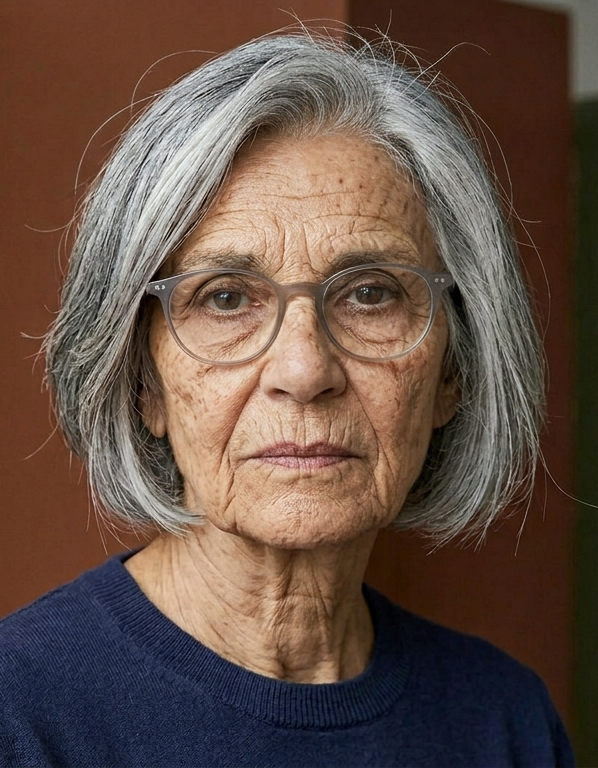
\includegraphics[width=\textwidth,height=5cm,keepaspectratio]
    {images/fatima.png}
    \vspace{0.2cm}
\end{minipage}
\hfill
\begin{minipage}[t]{0.70\textwidth}
    \begin{tcolorbox}[personabox]
        \textbf{\large Fatima Benali}\label{persona:fatima_benali} \\[4pt]
        {\color{secondaryColor}\small\textbf{Citazione significativa:}
        \textit{``Io non capisco le parole italiane scritte,
        ma so benissimo quale autobus prendere e dove scendere''}} \\[4pt]
        {\color{secondaryColor}\small\textbf{Segmento corrispondente:}
        Anziana straniera (68 anni, origine marocchina,
        alfabetizzata in arabo ma analfabeta in italiano scritto,
        competenza digitale minima, uso frequente del TPL)}
    \end{tcolorbox}
\end{minipage}

\vspace{0.3cm}

% ================================================================
% DESCRIZIONE DEL PERSONA (Basic Facts)
% ================================================================

\begin{tcolorbox}[base]
    \textbf{Descrizione del persona} \\[4pt]
    {\small
    \textbf{Età:} 68 anni \hfill
    \textbf{Genere:} Femmina \hfill
    \textbf{Nazionalità:} Marocchina, residente in Italia da 22 anni
    \\[2pt]
    \textbf{Residenza:} Bologna, quartiere Pilastro \hfill
    \textbf{Stato civile:} Coniugata \\[2pt]
    \textbf{Istruzione:} Scuola primaria completata in Marocco
    in lingua araba. Sa leggere e scrivere in arabo,
    ma non ha mai ricevuto alcuna istruzione in italiano. \\[2pt]
    \textbf{Competenza linguistica:} Italiano orale elementare
    (sufficiente per interazioni di routine: mercato, medico,
    sportello). Italiano scritto: nessuno. Non riconosce le
    lettere dell'alfabeto latino e non è in grado di leggere
    alcuna parola italiana, nemmeno le più comuni.
    Legge e scrive correttamente in arabo: usa WhatsApp
    in arabo per comunicare con i familiari in Marocco
    e con il gruppo del centro Al-Amal. \\[2pt]
    \textbf{Problemi fisici rilevanti:} Ipovisione lieve
    corretta con occhiali da vista. Motricità nella norma
    per l'età, senza limitazioni significative alle mani.
    Affaticamento visivo rapido davanti agli schermi. \\[2pt]
    \textbf{Profilo digitale:} Possiede uno smartphone Android
    acquistato dal figlio. Lo usa quotidianamente per
    videochiamate e messaggi su WhatsApp in arabo con
    i familiari in Marocco e con le amiche del centro Al-Amal.
    Non ha mai navigato su un sito web, non sa cosa sia
    un browser, non conosce il concetto di SPID né di ISEE.
    Non ha mai inserito dati in un modulo online. \\[2pt]
    \textbf{Utilizzo TPL:} Usa i mezzi TPER quasi ogni giorno
da oltre vent'anni per raggiungere il mercato, la moschea
del quartiere e il centro di aggregazione Al-Amal.
Ha un abbonamento mensile agevolato che fino ad oggi
il figlio Karim rinnovava allo sportello ogni mese.
Da quando il centro Al-Amal ha avviato uno sportello
di assistenza digitale con una volontaria dedicata,
Fatima si è rivolta a lei per le pratiche online.
Conosce perfettamente linee, fermate, coincidenze
e zone tariffarie dell'area in cui vive.
    }
\end{tcolorbox}

% ================================================================
% BACKGROUND E CARATTERISTICHE PSICOLOGICHE
% ================================================================

% ================================================================
% BACKGROUND — sostituire i paragrafi su Karim e sul contesto
% ================================================================

\begin{tcolorbox}[base]
    \textbf{Background e caratteristiche psicologiche} \\[4pt]
    {\small
    Fatima è arrivata in Italia nel 2003, raggiungendo il marito
    Rachid (operaio in pensione) già residente a Bologna.
    Ha sempre fatto la casalinga ed ha cresciuto tre figli
    in Italia: il maggiore, Karim (38 anni), lavora in un
    magazzino logistico con turni notturni; la seconda,
    Nadia (34 anni), vive a Modena con la propria famiglia;
    il più giovane, Youssef (28 anni), studia ingegneria
    a Bologna e vive fuori casa. Per anni è stato Karim
    a gestire tutte le pratiche burocratiche della famiglia,
    spesso in fretta tra un turno e l'altro. \\[4pt]

    Fatima sa leggere e scrivere in arabo, ma non ha mai
    imparato l'alfabeto latino: è cresciuta in Marocco dove
    l'istruzione era in arabo, e in 22 anni di vita in Italia
    non ha mai frequentato un corso di lingua strutturato.
    Comprende l'italiano parlato nelle situazioni quotidiane,
    ma davanti a una parola scritta in italiano è come
    trovarsi davanti a un codice sconosciuto:
    non riesce a decifrare nemmeno le lettere singole.
    Ha costruito una vita autonoma e dignitosa attraverso
    una straordinaria \textbf{memoria visiva e spaziale}:
    riconosce i luoghi per la forma degli edifici, i negozi
    per i colori delle insegne, gli autobus per il numero ---
    che ha imparato a riconoscere come forma visiva,
    non come simbolo linguistico.
    Sa orientarsi in tutta Bologna senza leggere un cartello. \\[4pt]

    Il punto di svolta nella vita digitale di Fatima
    è stato il centro Al-Amal. Da circa un anno,
    l'associazione ha avviato uno \textbf{sportello
    di assistenza digitale} gestito da Sara, una
    volontaria di 28 anni di seconda generazione,
    che parla arabo e italiano e conosce bene
    le procedure burocratiche locali. Sara non si
    sostituisce a Fatima: le siede accanto, indica
    lo schermo, aspetta che sia lei a toccare.
    In questo contesto strutturato --- sedute a un
    tavolo, senza la fretta di Karim tra un turno
    e l'altro --- Fatima si sente al sicuro e riesce
    a concentrarsi. Il centro è diventato il luogo
    dove Fatima impara, per imitazione e ripetizione,
    quello che fuori dal centro le sembra inaccessibile. \\[4pt]

    A differenza di Liliana, che sente attivamente la
    frustrazione della propria dipendenza digitale,
    Fatima la vive con \textbf{rassegnazione pragmatica}:
    considera normale che qualcuno la aiuti con queste cose,
    così come lei aiuta le altre donne del centro
    quando si tratta di orientarsi in città con i mezzi.
    Non percepisce ancora l'autonomia digitale come un
    obiettivo desiderabile. Tuttavia, quando Sara le mostra
    che potrebbe rinnovare l'abbonamento da sola
    senza aspettare nessuno, reagisce con curiosità genuina:
    \textit{``Ma si può davvero fare da sola?
    Nessuno me lo ha mai detto''}.
    }
\end{tcolorbox}

\vspace{0.3cm}

% ================================================================
% C&A DIAGRAM
% ================================================================

\begin{tcolorbox}[personabox]
    \textbf{Grafico delle competenze e abilità (C\&A Diagram)} \\[4pt]
    {\small
    }

    \vspace{0.3cm}

    \begin{center}
    \radarchart[primaryColor]{Fatima Benali}{2}{4}{1}{2}{3}{2}
    \end{center}

    \vspace{0.2cm}

    \begin{center}
    \renewcommand{\arraystretch}{1.3}
    \begin{tabular}{|l|c|c|}
        \hline
        \textbf{Dimensione} & \textbf{Punteggio (1--5)} & \textbf{Indicatore} \\
        \hline
        Competenza tecnica &
       \textbf{2} &
        \cellcolor{gray!10} \makebox[50pt]{\rule{10pt}{10pt}\rule{10pt}{10pt}\color{lightgray}\rule{10pt}{10pt}\rule{10pt}{10pt}\rule{10pt}{10pt}} \\
        \hline
        Competenza di dominio &
        \textbf{4} &
        \cellcolor{gray!10} \makebox[50pt]{\rule{10pt}{10pt}\rule{10pt}{10pt}\rule{10pt}{10pt}\rule{10pt}{10pt}\color{lightgray}\rule{10pt}{10pt}} \\
        \hline
        Competenza linguistica &
        \textbf{1} &
        \cellcolor{gray!10} \makebox[50pt]{\rule{10pt}{10pt}\color{lightgray}\rule{10pt}{10pt}\rule{10pt}{10pt}\rule{10pt}{10pt}\rule{10pt}{10pt}} \\
        \hline
        Abilità fisica e visiva &
        \textbf{3} &
        \cellcolor{gray!10} \makebox[50pt]{\rule{10pt}{10pt}\rule{10pt}{10pt}\rule{10pt}{10pt}\color{lightgray}\rule{10pt}{10pt}\rule{10pt}{10pt}} \\
        \hline
        Motivazione &
        \textbf{2} &
        \cellcolor{gray!10} \makebox[50pt]{\rule{10pt}{10pt}\rule{10pt}{10pt}\color{lightgray}\rule{10pt}{10pt}\rule{10pt}{10pt}\rule{10pt}{10pt}} \\
        \hline
        Concentrazione &
        \textbf{2} &
        \cellcolor{gray!10} \makebox[50pt]{\rule{10pt}{10pt}\rule{10pt}{10pt}\color{lightgray}\rule{10pt}{10pt}\rule{10pt}{10pt}\rule{10pt}{10pt}} \\
        \hline
    \end{tabular}
    \end{center}

    \vspace{0.2cm}
    {\small \textbf{Legenda:} \rule{10pt}{10pt} = valore raggiunto \hfill \color{lightgray}\rule{10pt}{10pt}\color{black} = valore non raggiunto}

    \vspace{0.3cm}
    {\small \textit{Nota: A differenza di Liliana (motivazione 3),
    che sente attivamente la frustrazione della dipendenza,
    Fatima la vive come condizione normale e inevitabile.
    La competenza di dominio alta (4) è invece una risorsa
    progettuale fondamentale: Fatima conosce già linee,
    fermate e zone tariffarie TPER. Se il design riesce ad agganciarsi
    a ciò che lei già sa --- numeri di linea, icone delle
    zone, colori delle fermate --- la curva di apprendimento
    si riduce drasticamente anche in presenza di una
    barriera linguistica strutturale.}}
\end{tcolorbox}

\vspace{0.3cm}

% ================================================================
% DETTAGLI INTERESSANTI ADDIZIONALI
% ================================================================

% ================================================================
% DETTAGLI INTERESSANTI — aggiornati al contesto Al-Amal
% ================================================================

\begin{tcolorbox}[base,colback=backgroundColor!50]
    \textbf{Dettagli interessanti addizionali} \\[4pt]
    {\small
    \begin{itemize}[leftmargin=*]
        \item Fatima legge e scrive correntemente in arabo
        e usa WhatsApp ogni giorno per messaggiare con
        i familiari rimasti in Marocco e con le amiche
        del centro Al-Amal. Ma davanti a una schermata
        in italiano è completamente disorientata:
        non riconosce le lettere, non può fare affidamento
        sul testo per orientarsi. Riconosce invece il logo
        TPER, i colori delle linee e i numeri degli autobus
        come forme visive consolidate dall'esperienza
        quotidiana. La sua mente elabora l'italiano
        per immagini, non per testo.

        \item Lo sportello digitale di Al-Amal ha un
        computer fisso con una connessione stabile e
        Sara che riceve il martedì e il giovedì pomeriggio.
        Fatima ha imparato a presentarsi nei giorni
        di Sara quando deve fare ``le cose sul computer''.
        Ha già completato due sessioni: nella prima
        ha imparato ad aprire il browser, nella seconda
        ha raggiunto la homepage di TPER. Il rinnovo
        dell'abbonamento sarà la terza sessione.

        \item Al centro Al-Amal ha imparato a usare
        WhatsApp guardando le altre donne farlo,
        senza che nessuno le spiegasse a parole.
        Impara per imitazione visiva e ripetizione,
        non per istruzione verbale: il modello di
        apprendimento più efficace per lei è
        ``guarda e ripeti'', non ``leggi e segui
        le istruzioni''. Sara ha adattato
        il proprio metodo di insegnamento
        a questo stile: mostra prima, parla dopo.

        \item Conserva i suoi documenti importanti
        (carta di soggiorno, tessera sanitaria,
        abbonamento TPER) in una busta trasparente
        ordinata per colore e dimensione. Non legge
        le etichette: riconosce i documenti dalla
        forma, dal colore e dalla foto.
        Sara le ha suggerito di portare sempre
        la busta alle sessioni: la tessera TPER
        sarà il punto di partenza per il flusso
        di rinnovo.
    \end{itemize}
    }
\end{tcolorbox}

% ================================================================
% USE CASE #1 (Scenario Rinnovo - Sessione di Training Guidata)
% ================================================================
\begin{tcolorbox}[sectionbox,colback=primaryColor!10]
    \textbf{Descrizione del Use Case \#1: Sessione di training guidata per il rinnovo dell'abbonamento mensile}
\end{tcolorbox}

\vspace{0.3cm}

% --- Use Case Narrative (technical, Scenari.pdf compliant) ---
\begin{tcolorbox}[base]
    {\small
    \textbf{Scenario:} Utente (competenza tecnica 2/5, competenza linguistica 1/5, analfabeta in alfabeto latino) tenta il rinnovo abbonamento mensile via browser in sessione di training con trainer umano presente.

    \textbf{Obiettivo:} Rinnovare abbonamento mensile TPER via web completando la procedura senza che il trainer prenda il controllo del dispositivo.

    \textbf{Sequenza:}
    \begin{enumerate}
        \item L'utente apre il browser e digita \texttt{tper.it}: operazione già esercitata, completata con successo in 10 sec.
        \item La homepage presenta layout denso (banner, notizie, carousel). L'utente fissa lo schermo senza riconoscere punti di ancoraggio visivi. Il trainer indica fisicamente: ``Qui.''
        \item L'utente clicca per imitazione spaziale. Il link reindirizza a \texttt{solweb.tper.it} senza segnalazione: interfaccia, colori e layout cambiano completamente. Nessun avviso.
        \item Il sistema richiede registrazione: modulo di 6 campi in italiano. Il trainer legge e traduce oralmente ogni campo.
        \item Campo CF: l'utente estrae la tessera sanitaria ma non individua il dato richiesto. Il trainer indica fisicamente la posizione sulla tessera e detta i 16 caratteri.
        \item Tempo accumulato per la registrazione: 7 minuti ($\sim$50\% della sessione). Quando il sistema richiede il numero tessera ``Mi Muovo'', l'utente non lo trova sulla carta. Il trainer indica il dato.
        \item Errore di battitura sul numero tessera: il sistema genera un messaggio di errore in italiano. L'utente non decifra il messaggio e non sa come correggere. Il trainer prende il mouse e corregge.
        \item Al pagamento, il trainer inserisce i dati della carta di credito. L'utente preme solo il pulsante finale di conferma.
    \end{enumerate}

    \textbf{Esito:} Rinnovo completato (successo operativo). L'utente non acquisisce competenze riproducibili: il trainer si è sostituito all'utente in 4 degli 8 passaggi. Il fallimento formativo è sistemico: la registrazione obbligatoria consuma le risorse attentive prima del task principale.

    \textbf{Tempi:} 15 minuti totali (7 minuti registrazione + 8 minuti rinnovo). La registrazione consuma il 50\% del tempo su un passaggio non necessario al task.
    }
\end{tcolorbox}

% ================================================================
% CONSIDERAZIONI CONCLUSIVE --- IMPATTO SUL DESIGN
% ================================================================
\begin{tcolorbox}[sectionbox,colback=primaryColor!10]
    \textbf{Considerazioni conclusive --- Impatto del persona e del caso d'uso sul design}
\end{tcolorbox}

\vspace{0.3cm}

\begin{tcolorbox}[base]
    {\small
    \textbf{Impatto del persona Fatima Benali sul design:} \\[4pt]
    Fatima \`e l'unico persona del cast che non legge l'alfabeto latino (competenza linguistica 1/5, concentrazione 2/5). Il suo profilo evidenzia i seguenti requisiti di design:

    \begin{itemize}[leftmargin=*]
        \item \textbf{RF-01 --- Interfaccia iconografica, non testuale:}
        Ogni etichetta, pulsante e messaggio in italiano \`e illeggibile per l'utente. L'interfaccia deve comunicare via icone, fotografie, colori e riferimenti visivi all'esperienza reale del trasporto pubblico, non via testo.

        \item \textbf{RF-02 --- Supporto all'apprendimento per imitazione visiva:}
        L'utente apprende per ``guarda e ripeti'', non per ``leggi e segui istruzioni''. Ogni flusso deve poter essere eseguito per imitazione spaziale, senza richiedere decodifica testuale.

        \item \textbf{RF-03 --- Riconoscimento visivo dei documenti:}
        Quando il sistema richiede un dato da un documento fisico, deve mostrare una riproduzione visiva del documento con indicazione grafica (freccia/evidenziatore) della posizione esatta del dato.

        \item \textbf{RF-04 --- Path minimo al task principale:}
        Ogni passaggio preliminare non essenziale (es. registrazione) consuma risorse attentive scarse. Il flusso deve minimizzare gli step prima dell'operazione target.
    \end{itemize}
    }
\end{tcolorbox}

\vspace{0.3cm}

\begin{tcolorbox}[base]
    {\small
    \textbf{Impatto del Use Case \#1 sul design:} \\[4pt]
    Anche con un trainer umano dedicato, il sistema attuale impedisce il trasferimento di competenze all'utente. Requisiti emersi:

    \begin{itemize}[leftmargin=*]
        \item \textbf{RF-05 --- Continuità visiva tra piattaforme:}
        Il passaggio da \texttt{tper.it} a \texttt{solweb.tper.it} deve essere segnalato all'utente con un indicatore di contesto (es. overlay ``Stai per passare al sito di acquisto''). L'interfaccia deve mantenere elementi visivi di continuità (colori, logo, layout familiare).

        \item \textbf{RF-06 --- Guest flow per operazioni semplici:}
        La registrazione obbligatoria per il rinnovo consuma il 50\% del tempo di sessione e tutta la capacità attentiva dell'utente. Operazioni semplici (rinnovo, verifica) devono essere accessibili senza registrazione.

        \item \textbf{RF-07 --- Supporto visivo alla compilazione:}
        Campi che richiedono dati da documenti fisici (numero tessera, CF) devono essere accompagnati da un'immagine del documento con indicazione visiva del dato richiesto.

        \item \textbf{RF-08 --- Errori non catastrofici:}
        I messaggi di errore devono utilizzare icone e linguaggio non verbale per comunicare la natura del problema a utenti che non leggono la lingua dell'interfaccia. Colore rosso da riservare a blocchi effettivi, non a errori di battitura.

        \item \textbf{RF-09 --- Modalità trainer con strumenti di guida:}
        Il sistema deve offrire una modalità che permetta a un trainer (umano o digitale) di evidenziare elementi, dettare passaggi e co-navigare senza fisicamente prendere il controllo del dispositivo.
    \end{itemize}
    }
\end{tcolorbox}

\vspace{0.3cm}

\end{center}

\begin{center}
    {\color{primaryColor}\Large\bfseries Persona and Use Case Card} \\[4pt]
    {\color{secondaryColor}\normalsize Phase B --- Feasibility Study} \\[4pt]
    {\color{secondaryColor}\small Questo persona non è il protagonista (cioè non è colui per cui stiamo progettando il nuovo strumento; `e un
membro del cast di supporto che però va comunque tenuto in considerazione per garantire un design inclusivo).}
\end{center}

\vspace{0.3cm}
{\color{borderColor}\hrule}
\vspace{0.5cm}

% ================================================================
% RIGA 1: FOTO + DATI ANAGRAFICI
% ================================================================

\begin{minipage}[t]{0.25\textwidth}
    \centering
    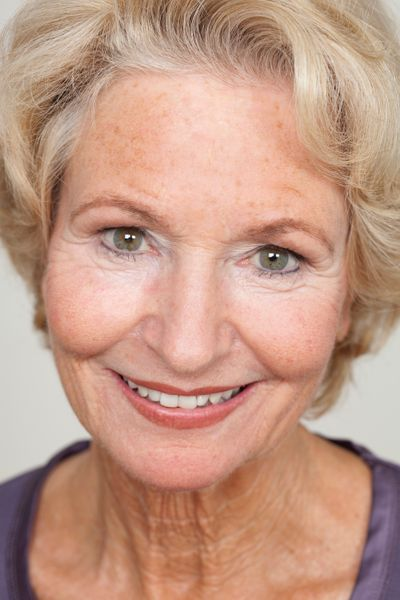
\includegraphics[width=\textwidth,height=5cm,keepaspectratio]{images/persona_protagonist.jpg}
    \vspace{0.2cm}
\end{minipage}
\hfill
\begin{minipage}[t]{0.70\textwidth}
    \begin{tcolorbox}[personabox]
        \textbf{\large Liliana Roversi} \\[4pt]
        {\color{secondaryColor}\small\textbf{Citazione significativa:} \textit{``Non so neanche da dove cominciare, per me queste cose le deve fare mia figlia.''}} \\[4pt]
        {\color{secondaryColor}\small\textbf{Segmento corrispondente:} Anziana pendolare (over 75, competenza digitale minima)}
    \end{tcolorbox}
\end{minipage}

\vspace{0.3cm}

% ================================================================
% DESCRIZIONE DEL PERSONA (Basic Facts)
% ================================================================

\begin{tcolorbox}[base]
    \textbf{Descrizione del persona} \\[4pt]
    {\small
    \textbf{Età:} 79 anni \hfill
    \textbf{Genere:} Femmina \hfill
    \textbf{Nazionalità:} Italiana \\[2pt]
    \textbf{Residenza:} Bologna, quartiere San Donato (periferia) \hfill
    \textbf{Stato civile:} Vedova, vive sola \\[2pt]
    \textbf{Istruzione:} Licenza elementare \\[2pt]
    \textbf{Problemi fisici rilevanti:} Presbiopia (utilizza occhiali da lettura), artrosi alle mani che riduce la motricità fine, ridotta mobilità (cammina con bastone per tragitti lunghi). \\[2pt]
    \textbf{Profilo digitale:} Possiede uno smartphone regalatole dalla figlia, ma lo usa esclusivamente per scrolling passivo su Facebook (foto di famiglia) e chiamate WhatsApp. Non ha mai utilizzato un browser per navigazione attiva, non ha mai compilato un modulo online. Durante i test è stata necessaria una fase di orientamento iniziale sul trackpad del computer. \\[2pt]
    \textbf{Utilizzo TPL:} Utente TPER da oltre 40 anni. Conosce bene le linee, le fermate e le zone tariffarie dell'esperienza fisica. Acquistava i biglietti in edicola e rinnovava l'abbonamento allo sportello TPER in stazione. Da quando molti servizi sono migrati online, dipende interamente dalla figlia per ogni operazione digitale.
    }
\end{tcolorbox}

% ================================================================
% BACKGROUND E CARATTERISTICHE PSICOLOGICHE
% ================================================================

\begin{tcolorbox}[base]
    \textbf{Background e caratteristiche psicologiche} \\[4pt]
    {\small
    Liliana è nata e cresciuta a Bologna, ha lavorato per 35 anni come collaboratrice scolastica in una scuola elementare del quartiere. È andata in pensione 14 anni fa. Suo marito, ex ferroviere, è deceduto 10 anni fa; da allora vive da sola in un appartamento al terzo piano senza ascensore. Ha due figli: la figlia maggiore, Elena (45 anni, impiegata comunale), vive in un comune limitrofo e la visita ogni martedì e sabato; il figlio minore, Marco (41 anni), vive a Milano e torna a Bologna una volta al mese. \\[4pt]

    Liliana è una donna orgogliosa e abituata all'autosufficienza: ha sempre gestito la casa, le finanze e le pratiche burocratiche in autonomia. La sua dipendenza dalla figlia per le operazioni digitali è per lei fonte di forte frustrazione e vergogna. Ha dichiarato: ``\textit{Mia figlia ha già i suoi problemi, non voglio essere un peso}''. \\[4pt]

    Psicologicamente, Liliana mostra un profondo \textbf{divario tra motivazione e autoefficacia}: vuole imparare, ma ogni tentativo fallito rafforza la convinzione di ``non essere portata'' per la tecnologia. Ha paura di ``rompere qualcosa'' o di ``fare un danno'' se clicca nel posto sbagliato. Preferisce non provare piuttosto che sbagliare e sentirsi umiliata. \\[4pt]

    È una persona metodica e paziente nella vita reale (ama il giardinaggio e la cucina, attività che richiedono precisione e ripetizione), ma l'ambiente digitale la disorienta: la densità di informazioni, le scelte multiple e la mancanza di un percorso fisico ``tattile'' le causano ansia e blocco decisionale.
    }
\end{tcolorbox}

\vspace{0.3cm}

% ================================================================
% C&A DIAGRAM (Radar chart — Competences and Abilities)
% ================================================================

\begin{tcolorbox}[personabox]
    \textbf{Grafico delle competenze e abilità (C\&A Diagram)} \\[4pt]
    {\small
    Ogni dimensione è valutata su una scala da 1 (molto bassa) a 5 (molto alta). \\
    I punteggi di Liliana riflettono il profilo emerso dai test utente e dalle osservazioni sul campo.
    }

    \vspace{0.3cm}

    \begin{center}
    \radarchart[accentOrange]{Liliana Roversi}{1}{3}{5}{3}{2}{2}
    \end{center}

    \vspace{0.2cm}

    \begin{center}
    \renewcommand{\arraystretch}{1.3}
    \begin{tabular}{|l|c|c|}
        \hline
        \textbf{Dimensione} & \textbf{Punteggio (1--5)} & \textbf{Indicatore} \\
        \hline
        Competenza tecnica &
        \textbf{1} &
        \cellcolor{gray!10} \makebox[50pt]{\rule{10pt}{10pt}\color{lightgray}\rule{10pt}{10pt}\rule{10pt}{10pt}\rule{10pt}{10pt}\rule{10pt}{10pt}} \\
        \hline
        Competenza di dominio &
        \textbf{3} &
        \cellcolor{gray!10} \makebox[50pt]{\rule{10pt}{10pt}\rule{10pt}{10pt}\rule{10pt}{10pt}\color{lightgray}\rule{10pt}{10pt}\rule{10pt}{10pt}} \\
        \hline
        Competenza linguistica &
        \textbf{5} &
        \cellcolor{gray!10} \makebox[50pt]{\rule{10pt}{10pt}\rule{10pt}{10pt}\rule{10pt}{10pt}\rule{10pt}{10pt}\rule{10pt}{10pt}} \\
        \hline
        Abilità fisica e visiva &
        \textbf{2} &
        \cellcolor{gray!10} \makebox[50pt]{\rule{10pt}{10pt}\rule{10pt}{10pt}\color{lightgray}\rule{10pt}{10pt}\rule{10pt}{10pt}\rule{10pt}{10pt}} \\
        \hline
        Motivazione &
        \textbf{3} &
        \cellcolor{gray!10} \makebox[50pt]{\rule{10pt}{10pt}\rule{10pt}{10pt}\rule{10pt}{10pt}\color{lightgray}\rule{10pt}{10pt}\rule{10pt}{10pt}} \\
        \hline
        Concentrazione &
        \textbf{2} &
        \cellcolor{gray!10} \makebox[50pt]{\rule{10pt}{10pt}\rule{10pt}{10pt}\color{lightgray}\rule{10pt}{10pt}\rule{10pt}{10pt}\rule{10pt}{10pt}} \\
        \hline
    \end{tabular}
    \end{center}

    \vspace{0.2cm}
    {\small \textbf{Legenda:} \rule{10pt}{10pt} = valore raggiunto \hfill \color{lightgray}\rule{10pt}{10pt}\color{black} = valore non raggiunto}
\end{tcolorbox}

\vspace{0.3cm}

% ================================================================
% DETTAGLI INTERESSANTI ADDIZIONALI
% ================================================================

\begin{tcolorbox}[base,colback=backgroundColor!50]
    \textbf{Dettagli interessanti addizionali} \\[4pt]
    {\small
    \begin{itemize}[leftmargin=*]
        \item Liliana ha un quaderno dove la figlia le scrive ``le istruzioni'' per le operazioni digitali, ma ogni volta che il sito cambia (anche di poco) le istruzioni non servono più e lei si blocca.
        \item Conserva ancora tutti i vecchi biglietti cartacei timbrati in un cassetto: per lei il ``ticket'' è un oggetto fisico, non un codice digitale.
        \item Parla al telefono con il figlio a Milano ogni sera, ma non ha mai provato a farsi spiegare qualcosa sullo smartphone al telefono --- ``tanto non capirei''.
        \item La domenica mattina va alla messa nella parrocchia del quartiere, dove si ferma a parlare con altre anziane del quartiere. Molte condividono la sua stessa frustrazione digitale, ma nessuna sa come uscirne.
    \end{itemize}
    }
\end{tcolorbox}

\newpage

% ================================================================
% USE CASE #1: «Il passaggio fantasma»
% ================================================================

\begin{tcolorbox}[sectionbox,colback=primaryColor!10]
    \textbf{Descrizione del Use Case \#1: Tentativo di rinnovo dell'abbonamento mensile --- il passaggio fantasma tra tper.it e solweb.tper.it}
\end{tcolorbox}

\vspace{0.3cm}

% --- Narrative ---
\begin{tcolorbox}[base]
    {\small
    \textbf{Scenario:} Utente (competenza tecnica 1/5, concentrazione 2/5) tenta il rinnovo dell'abbonamento mensile via web in completa autonomia. L'intermediario abituale (figlia) non è disponibile. Scadenza: domani.

    \textbf{Obiettivo:} Rinnovare l'abbonamento mensile TPER via web senza assistenza umana.

    \textbf{Sequenza:}
    \begin{enumerate}
        \item L'utente apre il browser, digita \texttt{tper.it} nella barra di ricerca Google invece che nella barra indirizzi: errore di riconoscimento dell'interfaccia. Al secondo tentativo raggiunge la homepage.
        \item La homepage presenta notizie, avvisi, banner e carousel senza una gerarchia visiva tra contenuto informativo e azione transazionale. L'utente scansiona la pagina per 45 sec prima di individuare la voce ``Abbonamenti'' nel menu in alto.
        \item L'utente clicca ``Abbonamenti'' $\rightarrow$ ``Mensile'' $\rightarrow$ ``Acquista''. Il link reindirizza a \texttt{solweb.tper.it} senza segnalazione. L'interfaccia cambia completamente (colori, layout, dominio).
        \item Il sistema richiede login. L'utente non ha un account. Cerca un pulsante ``Continua senza registrazione'': assente.
        \item L'utente tenta ``Registrati'': modulo di 6+ campi obbligatori (nome, cognome, email, password, conferma, termini). Prova a compilare, sbaglia, cancella, riprova per 5 minuti.
        \item Dopo l'ennesimo errore, l'utente chiude il browser. Contatta l'intermediario: ``Non ci sono riuscita. Me lo fai tu?''
    \end{enumerate}

    \textbf{Barriere:}
    \begin{itemize}
        \item Riconoscimento barra indirizzi vs. barra di ricerca (competenza tecnica 1/5).
        \item Passaggio \texttt{tper.it} $\rightarrow$ \texttt{solweb.tper.it} non segnalato: cambio di piattaforma senza contesto.
        \item Nessun percorso guest: registrazione obbligatoria anche per operazioni semplici.
        \item Form di registrazione esteso: 6+ campi, requisiti di complessità password non comunicati.
        \item Errore generico: il sistema segnala l'errore ma non indica come correggere.
    \end{itemize}

    \textbf{Esito:} Operazione non completata. L'intermediario esegue il task al posto dell'utente. Ciclo di dipendenza perpetuato. Nessuna competenza trasferita.

    \textbf{Tempi:} 15 minuti tentativo autonomo + 10 minuti intervento intermediario.
    }
\end{tcolorbox}

\vspace{0.3cm}

% ================================================================
% USE CASE #2: «L'architettura labirinto»
% ================================================================

\begin{tcolorbox}[sectionbox,colback=primaryColor!10]
    \textbf{Descrizione del Use Case \#2: Tentativo fallito di rinnovo --- l'architettura informativa labirinto e l'assenza di modalità trainer}
\end{tcolorbox}

\vspace{0.3cm}

\begin{tcolorbox}[base]
    {\small
    \textbf{Scenario:} Utente (competenza tecnica 1/5, motivazione 3/5) tenta il rinnovo con assistenza di un intermediario (figlia) che funge da trainer. Obiettivo dichiarato: apprendere la procedura per futura autonomia.

    \textbf{Obiettivo:} Rinnovare abbonamento mensile TPER con assistenza trainer, trasferendo competenze per autonomia futura.

    \textbf{Sequenza:}
    \begin{enumerate}
        \item Homepage: layout informativo (notizie, avvisi, banner) prevale su azioni transazionali. L'utente fissa lo schermo: ``Non so dove guardare.'' Il trainer indica il menu.
        \item Menu: 7+ voci di primo livello. L'utente esita su ciascuna. Il trainer guida: ``Abbonamenti'' $\rightarrow$ ``Mensile''. La pagina descrive le tariffe; il pulsante ``Acquista online'' è oltre la piega dello schermo. L'utente non sa che deve scrollare.
        \item Click $\rightarrow$ reindirizzamento a \texttt{solweb.tper.it}: interfaccia, colori e layout cambiano completamente. Nessuna segnalazione. Il trainer spiega la transizione.
        \item Il sistema richiede login/registrazione. Il trainer tenta la registrazione guidata. Campo password: requisiti di complessità non comunicati chiaramente. Errori ripetuti.
        \item Dopo 3 tentativi di password falliti, l'utente cede: ``Tanto lo fai tu.'' Il trainer completa la registrazione e l'acquisto.
    \end{enumerate}

    \textbf{Esito:} L'utente non esegue nessun passaggio in autonomia. Training bloccato da: (1) homepage non orientata all'azione, (2) IA a $\geq$5 livelli di profondità, (3) registrazione obbligatoria per rinnovo. Il trainer si sostituisce all'utente. Autoefficacia percepita peggiorata.

    \textbf{Tempi:} 25 minuti sessione training + acquisto. Zero competenze trasferite.
    }
\end{tcolorbox}

\newpage

% ================================================================
% 

% IMPATTO DEL PERSONA E DEGLI USE CASE SUL DESIGN
% ================================================================

\begin{tcolorbox}[sectionbox,colback=primaryColor!10]
    \textbf{Considerazioni conclusive --- Impatto del persona e dei casi d'uso sul design}
\end{tcolorbox}

\vspace{0.3cm}

\begin{tcolorbox}[base]
    {\small
    \textbf{Impatto del persona Liliana Roversi sul design:} \\[4pt]
    Profilo: competenza tecnica 1/5, motivazione 3/5, concentrazione 2/5. Requisiti emersi:

    \begin{itemize}[leftmargin=*]
        \item \textbf{RF-10 --- Separazione netta tra contenuto informativo e azione transazionale (cfr. D1):} La homepage deve distinguere visivamente le aree ``informazione'' (notizie, avvisi) da quelle ``operazione'' (rinnovo, acquisto, verifica), offrendo percorsi d'azione immediatamente riconoscibili anche a utenti con competenza tecnica minima.

        \item \textbf{RF-11 --- Architettura informativa piatta per flussi operativi (cfr. D2):} I flussi transazionali (rinnovo, acquisto) non devono richiedere più di 3 click dal punto di ingresso. Voci di menu oltre il secondo livello vanno riservate a contenuti informativi, non operativi.

        \item \textbf{RF-12 --- Modalità co-navigazione trainer/utente (cfr. R5):} Il sistema deve offrire una vista condivisa che permetta al trainer di evidenziare elementi, dettare passaggi e guidare senza prendere fisicamente il controllo del dispositivo (es. overlay di puntamento, step evidenziati).

        \item \textbf{RF-13 --- Ponte analogico-digitale (cfr. R3, R6):} L'utente deve poter ricevere output stampabili (promemoria cartacei, QR code, calendario scadenze) per mantenere un aggancio con le abitudini analogiche preesistenti.
    \end{itemize}
    }
\end{tcolorbox}

\vspace{0.3cm}

\begin{tcolorbox}[base]
    {\small
    \textbf{Impatto del Use Case \#1 (Il passaggio fantasma) sul design:} \\[4pt]
    \begin{itemize}[leftmargin=*]
        \item \textbf{RF-14 --- Segnalazione cambio piattaforma (cfr. R4):} Il passaggio \texttt{tper.it} $\rightarrow$ \texttt{solweb.tper.it} deve essere segnalato con un indicatore di contesto (banner, overlay, nota visiva). L'utente deve sapere di aver cambiato ambiente e perché.

        \item \textbf{RF-15 --- Guest flow per rinnovo senza registrazione (cfr. D5):} Un rinnovo di abbonamento non richiede identificazione preventiva. Il sistema deve offrire un percorso guest che richieda solo i dati essenziali alla transazione (numero tessera + pagamento), senza obbligo di account.
    \end{itemize}
    \vspace{0.2cm}
    \textbf{Impatto del Use Case \#2 (L'architettura labirinto) sul design:} \\[4pt]
    \begin{itemize}[leftmargin=*]
        \item \textbf{RF-16 --- Deep link diretto alle azioni (cfr. D2):} Ogni operazione deve essere raggiungibile con $\leq$3 click dalla homepage. La homepage deve esporre le azioni principali (rinnovo, acquisto, verifica) come card primarie, non come voci di sottomenu.

        \item \textbf{RF-17 --- Gerarchia visiva homepage orientata all'azione (cfr. D1):} Le azioni transazionali devono essere visivamente distinte dai contenuti informativi, con peso visivo maggiore e priorità di layout (es. sezione ``Operazioni rapide'' in hero, notizie in footer/secondary).
    \end{itemize}
    }
\end{tcolorbox}

\begin{center}
    {\color{primaryColor}\Large\bfseries Persona and Use Case Card} \\[4pt]
    {\color{secondaryColor}\normalsize Phase B --- Feasibility Study} \\[4pt]
    {\color{secondaryColor}\small Questo \textit{persona} \textbf{non} \`e il protagonista (cio\`e non \`e colui per cui stiamo progettando il nuovo strumento; \`e un membro del cast di supporto che per\`o va comunque tenuto in considerazione per garantire un design inclusivo).}
\end{center}

\vspace{0.3cm}
{\color{borderColor}\hrule}
\vspace{0.5cm}

% ================================================================
% RIGA 1: FOTO + DATI ANAGRAFICI
% ================================================================

\begin{minipage}[t]{0.25\textwidth}
    \centering
    
\includegraphics[width=\textwidth,height=5cm,keepaspectratio]{images/persona_nonprotagonist.jpg}
    \vspace{0.2cm}
    {\small\itshape Foto di repertorio}
\end{minipage}
\hfill
\begin{minipage}[t]{0.70\textwidth}
    \begin{tcolorbox}[personabox]
        \textbf{\large David Carter} \\[4pt]
        {\color{secondaryColor}\small\textbf{Citazione significativa:} \textit{``I can find the timetable, but once I need to buy or renew something, the process becomes harder to follow and I need clearer guidance in English.''}} \\[4pt]
        {\color{secondaryColor}\small\textbf{Segmento corrispondente:} Lavoratore straniero (18--35, competenza digitale media, contesto associativo)}
    \end{tcolorbox}
\end{minipage}

\vspace{0.3cm}

% ================================================================
% DESCRIZIONE DEL PERSONA (Basic Facts)
% ================================================================

\begin{tcolorbox}[base]
    \textbf{Descrizione del persona} \\[4pt]
    {\small
    \textbf{Et\`a:} 32 anni \hfill
    \textbf{Genere:} Maschio \hfill
    \textbf{Nazionalit\`a:} Britannica (madrelingua inglese) \\[2pt]
    \textbf{Residenza:} Bologna, zona San Vitale (vicino universit\`a) \hfill
    \textbf{Stato civile:} Single, vive in un appartamento condiviso con altri due colleghi \\[2pt]
    \textbf{Istruzione:} Laurea in Ingegneria Meccanica (Regno Unito) \\[2pt]
    \textbf{Professione:} Ingegnere presso una multinazionale con sede a Bologna (distaccato per 12 mesi) \\[2pt]
    \textbf{Problemi fisici rilevanti:} Nessuno. \\[2pt]
    \textbf{Profilo digitale:} Utilizza quotidianamente smartphone, email, Google Maps, app bancarie e servizi di acquisto online in inglese. Ha familiarit\`a con la navigazione web avanzata, i sistemi di autenticazione a due fattori e il mobile payment del suo paese d'origine. Tuttavia non ha mai utilizzato un portale della pubblica amministrazione italiana e non sa come funzioni la bigliettazione digitale del TPL locale. \\[2pt]
    \textbf{Utilizzo TPL:} Usa il TPER quotidianamente per spostarsi tra casa, sede di lavoro (Zona Roveri) e centro. Ha acquistato biglietti singoli tramite app e rivenditori autorizzati, ma non ha mai completato un rinnovo abbonamento online. Non sa quali agevolazioni tariffarie esistano per stranieri o residenti temporanei.
    }
\end{tcolorbox}

\newpage

% ================================================================
% BACKGROUND E CARATTERISTICHE PSICOLOGICHE
% ================================================================

\begin{tcolorbox}[base]
    \textbf{Background e caratteristiche psicologiche} \\[4pt]
    {\small
    David \`e arrivato a Bologna da circa due mesi per un distacco lavorativo presso la sede italiana della sua azienda. Parla un italiano scolastico di livello base (A2/B1) -- sufficiente per interazioni semplici ma non per comprendere etichette tecniche, testi burocratici o moduli online complessi. \\[4pt]

    \`E una persona abituata all'autonomia digitale: nel Regno Unito gestisce ogni aspetto della sua mobilit\`a online (biglietti ferroviari, abbonamenti metropolitana, ticket bus) attraverso app intuitive e siti ben progettati. L'esperienza con TPER lo frustra perch\'e segue le stesse strategie di navigazione che funzionano a Londra ma si scontrano con un'interfaccia che presume conoscenza del contesto italiano (MI MUOVO, Io Viaggio, Carta Agevolata, ISEE). \\[4pt]

    Psicologicamente, David mostra un \textbf{divario tra competenza tecnica e competenza di dominio}: sa usare perfettamente la tecnologia, ma non ha il contesto culturale per interpretare il sistema italiano. Questo genera un senso di impotenza specifica -- non ``non so usare il computer'' ma ``non capisco cosa mi stanno chiedendo''. La barriera non \`e emotiva (non ha paura di sbagliare) ma \textbf{cognitivo-linguistica}: non ha gli strumenti lessicali e sistemici per decodificare l'interfaccia. \\[4pt]

    Ha un atteggiamento pratico e determinato: quando incontra un ostacolo cerca attivamente una soluzione (chiede aiuto a colleghi italiani, cerca su Google, prova percorsi alternativi). Tuttavia, dopo ripetuti fallimenti sui flussi transazionali, inizia a mostrare segni di \textbf{affaticamento decisionale} -- troppi passaggi, troppi termini sconosciuti, troppe scelte senza contesto.
    }
\end{tcolorbox}

\vspace{0.3cm}

% ================================================================
% C&A DIAGRAM (Competences and Abilities)
% ================================================================

\begin{tcolorbox}[personabox]
    \textbf{Grafico delle competenze e abilit\`a (C\&A Diagram)} \\[4pt]
    {\small
    Ogni dimensione \`e valutata su una scala da 1 (molto bassa) a 5 (molto alta). \\
    I punteggi di David riflettono il profilo emerso dai test utente e dalle osservazioni sul campo.
    }

    \vspace{0.3cm}

    \begin{center}
    \radarchart[accentGreen]{David Carter}{4}{2}{2}{4}{5}{3}
    \end{center}

    \vspace{0.2cm}

    \begin{center}
    \renewcommand{\arraystretch}{1.3}
    \begin{tabular}{|l|c|c|}
        \hline
        \textbf{Dimensione} & \textbf{Punteggio (1--5)} & \textbf{Indicatore} \\
        \hline
        Competenza tecnica &
        \textbf{4} &
        \cellcolor{gray!10} \makebox[50pt]{\rule{10pt}{10pt}\rule{10pt}{10pt}\rule{10pt}{10pt}\rule{10pt}{10pt}\color{lightgray}\rule{10pt}{10pt}} \\
        \hline
        Competenza di dominio &
        \textbf{2} &
        \cellcolor{gray!10} \makebox[50pt]{\rule{10pt}{10pt}\rule{10pt}{10pt}\color{lightgray}\rule{10pt}{10pt}\rule{10pt}{10pt}\rule{10pt}{10pt}} \\
        \hline
        Competenza linguistica &
        \textbf{2} &
        \cellcolor{gray!10} \makebox[50pt]{\rule{10pt}{10pt}\rule{10pt}{10pt}\color{lightgray}\rule{10pt}{10pt}\rule{10pt}{10pt}\rule{10pt}{10pt}} \\
        \hline
        Abilit\`a fisica e visiva &
        \textbf{5} &
        \cellcolor{gray!10} \makebox[50pt]{\rule{10pt}{10pt}\rule{10pt}{10pt}\rule{10pt}{10pt}\rule{10pt}{10pt}\rule{10pt}{10pt}} \\
        \hline
        Motivazione &
        \textbf{4} &
        \cellcolor{gray!10} \makebox[50pt]{\rule{10pt}{10pt}\rule{10pt}{10pt}\rule{10pt}{10pt}\rule{10pt}{10pt}\color{lightgray}\rule{10pt}{10pt}} \\
        \hline
        Concentrazione &
        \textbf{3} &
        \cellcolor{gray!10} \makebox[50pt]{\rule{10pt}{10pt}\rule{10pt}{10pt}\rule{10pt}{10pt}\color{lightgray}\rule{10pt}{10pt}\rule{10pt}{10pt}} \\
        \hline
    \end{tabular}
    \end{center}

    \vspace{0.2cm}
    {\small \textbf{Legenda:} \rule{10pt}{10pt} = valore raggiunto \hfill \color{lightgray}\rule{10pt}{10pt}\color{black} = valore non raggiunto}
\end{tcolorbox}

\vspace{0.3cm}

% ================================================================
% DETTAGLI INTERESSANTI ADDIZIONALI

\newpage

% ================================================================
% USE CASE #1: «Il rinnovo che non si vede»
% ================================================================

\begin{tcolorbox}[sectionbox,colback=primaryColor!10]
    \textbf{Descrizione del Use Case \#1: Rinnovo dell'abbonamento online concluso con successo ma sanzionato a bordo --- il post-acquisto non spiegato}
\end{tcolorbox}

\vspace{0.3cm}

% --- Narrative ---
\begin{tcolorbox}[base]
    {\small
    \textbf{Scenario:} Utente (competenza tecnica 4/5, competenza linguistica 2/5, competenza di dominio 2/5) ha già un account su \texttt{solweb.tper.it} creato con assistenza. Tenta il rinnovo in autonomia.

    \textbf{Obiettivo:} Rinnovare abbonamento mensile TPER e utilizzarlo correttamente a bordo.

    \textbf{Sequenza:}
    \begin{enumerate}
        \item L'utente apre \texttt{solweb.tper.it}, fa login (procedura familiare), naviga a ``Rinnovo abbonamento mensile'' e completa il pagamento con carta di credito. Tempo: 5 minuti. Operazione lineare.
        \item Il sistema mostra ``Pagamento riuscito'' e invia email con ricevuta PDF. Nessun messaggio aggiuntivo su come rendere valido il titolo a bordo. L'utente salva la ricevuta sul telefono.
        \item Il giorno dopo, l'utente sale sull'autobus. Al controllo, mostra la ricevuta PDF. Il controllore rifiuta: ``L'abbonamento va caricato su Mi Muovo o sull'app TPER. Questa è solo la ricevuta.''
        \item Il controllore emette sanzione di 60\euro{} per viaggio senza titolo valido. L'utente ha pagato 50\euro{} per l'abbonamento e riceve 60\euro{} di multa.
        \item Post-evento: l'utente consulta un collega italiano e scopre la procedura di attivazione mai comunicata durante il checkout. Il flusso di acquisto non ha mai menzionato il passaggio di caricamento.
    \end{enumerate}

    \textbf{Barriere:}
    \begin{itemize}
        \item \textbf{RF-18} --- Il checkout termina con la conferma di pagamento senza istruire su come rendere valido l'abbonamento a bordo.
        \item \textbf{RF-19} --- Frammentazione ecosistema (solweb = acquisto, Mi Muovo = supporto fisico, app TPER = digitale) mai esplicitata all'utente.
        \item \textbf{RF-20} --- Nessun messaggio durante l'acquisto su passaggi post-pagamento.
    \end{itemize}

    \textbf{Esito:} Acquisto completato (successo transazionale). Utilizzo fallito (fallimento esperienziale). Danno economico: 60\euro{} multa + 50\euro{} abbonamento = 110\euro{} totali per un servizio da 50\euro{}.

    \textbf{Tempi:} 15 minuti acquisto + 10 minuti controllo + 15 minuti spiegazione intermediario.
    }
\end{tcolorbox}

\vspace{0.3cm}

% ================================================================
% USE CASE #2: «L'agevolazione nascosta»
% ================================================================

\begin{tcolorbox}[sectionbox,colback=primaryColor!10]
    \textbf{Descrizione del Use Case \#2: Ricerca di agevolazioni tariffarie --- informazioni opache e lingua assente nascondono sconti reali}
\end{tcolorbox}

\vspace{0.3cm}

\begin{tcolorbox}[base]
    {\small
    \textbf{Scenario:} Utente (competenza linguistica 2/5, competenza di dominio 2/5) paga abbonamento a prezzo pieno (50\euro{}/mese) da 3 mesi. Un collega lo informa di tariffe agevolate per ISEE sotto 16.000\euro{}. L'utente non conosce ISEE, Carta Agevolata, DSU.

    \textbf{Obiettivo:} Scoprire se ha diritto a sconti o agevolazioni sull'abbonamento mensile TPER.

    \textbf{Sequenza:}
    \begin{enumerate}
        \item L'utente cerca ``discount'' nella barra di ricerca di \texttt{tper.it}: 0 risultati. Prova ``sconti'': 0. Prova ``agevolazioni'': pagine con titoli ``Carta Agevolata'', ``ISEE'', ``DSU'' --- termini non tradotti e privi di contesto per un utente straniero.
        \item L'utente naviga il menu: ``Abbonamenti'' $\rightarrow$ ``Agevolazioni''. Pagina con testo burocratico italiano denso: requisiti, soglie, delibere. Nessun selettore lingua presente.
        \item L'utente tenta Google Translate: gli acronimi (ISEE, DSU) restano invariati. ``Carta Agevolata'' tradotta letteralmente, senza spiegazione del significato.
        \item Dopo 15 minuti di tentativi, l'utente abbandona. Il giorno dopo chiede al collega, che verifica: l'utente ha diritto a tariffa agevolata (30\euro{} invece di 50\euro{}).
    \end{enumerate}

    \textbf{Barriere:}
    \begin{itemize}
        \item \textbf{RF-21} --- Ricerca interna non supporta sinonimi o intenti (``discount'' $\neq$ ``agevolazioni'').
        \item \textbf{RF-22} --- Termini burocratici (ISEE, DSU) non spiegati: nessun tooltip/glossario.
        \item \textbf{RF-23} --- Pagine informative non disponibili in inglese. Google Translate inefficace su acronimi.
    \end{itemize}

    \textbf{Esito:} Informazione non scoperta in autonomia. L'utente subisce una perdita economica di 60\euro{} in 3 mesi (150\euro{} pagati contro 90\euro{} dovuti), attribuibile all'opacità informativa del sito.

    \textbf{Costo opacità:} 60\euro{} in 3 mesi (20\euro{}/mese di extra costo).
    }
\end{tcolorbox}

\vspace{0.3cm}

% ================================================================
% IMPATTO DEL PERSONA E DEGLI USE CASE SUL DESIGN
% ================================================================

\begin{tcolorbox}[sectionbox,colback=primaryColor!10]
    \textbf{Considerazioni conclusive --- Impatto del persona e dei casi d'uso sul design}
\end{tcolorbox}
\vspace{0.3cm}

\begin{tcolorbox}[base]
    {\small
    \textbf{Impatto del persona David Carter sul design:} \\[4pt]
    Profilo: competenza tecnica 4/5, competenza di dominio 2/5, competenza linguistica 2/5. Requisiti emersi:

    \begin{itemize}[leftmargin=*]
        \item \textbf{RF-24 --- Glossario contestuale per terminologia di dominio (cfr. D3):} Termini come ``Mi Muovo'', ``Codice Fiscale'', ``ISEE'', ``DSU'', ``Carta Agevolata'' devono essere accompagnati da tooltip esplicativi e, per utenti non italiani, da traduzioni contestuali. Per competenza linguistica 2/5, i termini non spiegati bloccano il flusso.

        \item \textbf{RF-25 --- Supporto multilingua nei flussi di registrazione e acquisto (cfr. R12):} L'interfaccia inglese su \texttt{solweb.tper.it} deve essere disponibile \textit{prima} del login, non dopo. L'utente straniero necessita della lingua straniera proprio durante la registrazione e il primo accesso.

        \item \textbf{RF-26 --- Motore di ricerca per intenti (cfr. R2):} La ricerca interna deve supportare sinonimi e query semantiche (``discount'', ``sconti'', ``monthly pass'') oltre alla terminologia burocratica esatta. Per un utente che non conosce il dominio, formulare la query giusta non deve essere un prerequisito.

        \item \textbf{RF-27 --- Contenuti informativi in lingua chiara (cfr. D2, R3):} Le pagine descrittive (abbonamenti, agevolazioni) devono utilizzare un tono non burocratico, spiegando i concetti normativi (ISEE, DSU, delibere) in linguaggio accessibile anche a chi non ha familiarità con il contesto istituzionale italiano.
    \end{itemize}
    }
\end{tcolorbox}

\vspace{0.3cm}

\begin{tcolorbox}[base]
    {\small
    \textbf{Impatto del Use Case \#1 (Il rinnovo che non si vede) sul design:} \\[4pt]
    \begin{itemize}[leftmargin=*]
        \item \textbf{RF-28 --- Guida procedurale post-acquisto obbligatoria (cfr. R10):} Il flusso di checkout non deve concludersi al pagamento. Deve includere una schermata ``Istruzioni per l'uso'' che spieghi come rendere l'abbonamento valido a bordo (caricamento su Mi Muovo/app TPER). La ricevuta email deve essere accompagnata da istruzioni procedurali chiare.

        \item \textbf{RF-29 --- Mappatura esplicita dell'ecosistema multipiattaforma (cfr. D5, R4):} Il sistema deve dichiarare esplicitamente le relazioni tra piattaforme (solweb = acquisto, Mi Muovo = supporto fisico, app TPER = digitale) al momento opportuno, non a posteriori. L'utente deve sapere su quale piattaforma sta operando e cosa succede dopo.

        \item \textbf{Costo della mancata guida:} Una multa di 60\euro{} per un abbonamento pagato 50\euro{} (danno >100\% del valore della transazione) è una conseguenza economica inaccettabile generata esclusivamente dall'opacit\`a procedurale del sistema.
    \end{itemize}
    \vspace{0.2cm}
    \textbf{Impatto del Use Case \#2 (L'agevolazione nascosta) sul design:} \\[4pt]
    \begin{itemize}[leftmargin=*]
        \item \textbf{RF-30 --- Ricerca semantica e per intenti (cfr. R2):} Il motore di ricerca interno deve restituire risultati per ``discount'', ``sconti'', ``risparmio'' oltre che per ``agevolazioni''. Per un utente con competenza linguistica 2/5 e competenza di dominio 2/5, conoscere il termine burocratico esatto non può essere un prerequisito.

        \item \textbf{RF-31 --- Equità informativa: terminologia spiegata (cfr. D3):} Termini burocratici (ISEE, DSU) devono essere accompagnati da spiegazioni in linguaggio semplice, tooltip e traduzioni. L'opacit\`a terminologica colpisce selettivamente gli utenti che più hanno bisogno delle agevolazioni, configurando un problema di equità oltre che di usabilità.

        \item \textbf{RF-32 --- Pagine informative in inglese (cfr. R12):} Le pagine su tariffe e agevolazioni devono essere disponibili in inglese. Google Translate non traduce acronimi burocratici, rendendo le informazioni su agevolazioni di fatto invisibili per chi non parla italiano.
    \end{itemize}
    }
\end{tcolorbox}
\begin{center}
    {\color{primaryColor}\Large\bfseries Persona and Use Case Card} \\[4pt]
    {\color{secondaryColor}\normalsize Phase B --- Feasibility Study} \\[4pt]
    {\color{secondaryColor}\small Questo \textit{persona} \textbf{non} \`e il protagonista (cio\`e non \`e colui per cui stiamo progettando il nuovo strumento; \`e un membro del cast di supporto che per\`o va comunque tenuto in considerazione per garantire un design inclusivo).}
\end{center}

\vspace{0.3cm}
{\color{borderColor}\hrule}
\vspace{0.4cm}

\begin{minipage}[t]{0.25\textwidth}
    \centering
    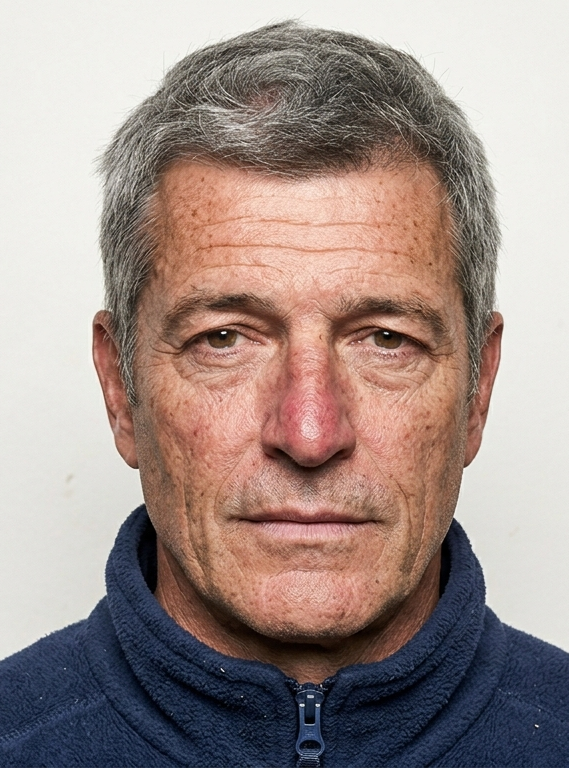
\includegraphics[width=\textwidth,height=5cm,keepaspectratio]
    {images/roberto.png}
    \vspace{0.2cm}
\end{minipage}
\hfill
\begin{minipage}[t]{0.70\textwidth}
    \begin{tcolorbox}[personabox]
        \textbf{\large Roberto Rinaldi}\label{persona:roberto_rinaldi} \\[4pt]
        {\color{secondaryColor}\small\textbf{Citazione significativa:}
        \textit{``Sinceramente, mettermi al computer a leggere pagine e pagine di istruzioni mi fa passare la voglia. Preferisco andare allo sportello così fa tutto l'operatore, anche se un po' mi imbarazza dover fare mille domande se c'è molta fila.''}} \\[4pt]
        {\color{secondaryColor}\small\textbf{Segmento corrispondente:}
        \hyperref[seg:cittadino]{[S3]} Il cittadino allo sportello (Italiano, 36--64 anni, competenza digitale bassa, relazione istituzionale e occasionale con TPER, forte bisogno di assistenza fisica).}
    \end{tcolorbox}
\end{minipage}

\vspace{0.3cm}

% ================================================================
% DESCRIZIONE DEL PERSONA (Basic Facts)
% ================================================================

\begin{tcolorbox}[base]
    \textbf{Descrizione del persona} \\[4pt]
    {\small
    \textbf{Età:} 54 anni \hfill
    \textbf{Genere:} Maschio \hfill
    \textbf{Nazionalità:} Italiana
    \\[2pt]
    \textbf{Residenza:} Bologna, quartiere periferico (Borgo Panigale) \hfill
    \textbf{Stato civile:} Separato \\[2pt]
    \textbf{Professione e Reddito:} Collaboratore scolastico (personale ATA) con contratto a tempo determinato. Ha un ISEE basso dovuto al recente periodo di disoccupazione e all'affitto che paga per una piccola stanza in condivisione. \\[2pt]
    \textbf{Competenza linguistica:} Madrelingua italiano. Comprende perfettamente la lingua, ma si annoia subito di fronte al linguaggio burocratico e ai muri di testo densi tipici dei siti istituzionali, preferendo evitare lo sforzo di leggerli e interpretarli. \\[2pt]
    \textbf{Problemi fisici rilevanti:} Nessun problema motorio grave; soffre di una leggera presbiopia (usa occhiali da lettura per vedere da vicino) e di alcuni acciacchi alla schiena causati dai lavori manuali svolti in passato. \\[2pt]
    \textbf{Profilo digitale:} Possiede uno smartphone di fascia bassa che usa per telefonare, mandare messaggi su WhatsApp ai figli e guardare qualche video o notizia. Non soffre di fobie tecnologiche o ansie legate alla sicurezza informatica, ma è estremamente pigro nell'apprendimento digitale: se una procedura richiede più di due passaggi o l'applicazione mentale su moduli strutturati, si stufa e abbandona. Non ha attivato lo SPID semplicemente perché ha continuato a rimandare la trafila, trovandola una noiosa perdita di tempo. \\[2pt]
    \textbf{Utilizzo TPL:} Fino a tre mesi fa usava solo l'automobile. Arrivato a Bologna, si è trovato senza macchina e deve affidarsi completamente agli autobus per andare a scuola. Al momento paga biglietti singoli o giornalieri, sprecando molto denaro, e non possiede ancora un abbonamento. Rimanda costantemente l'acquisto per pura inerzia, non conoscendo ancora bene le linee o le regole tariffarie del servizio.
    }
\end{tcolorbox}

\vspace{0.3cm}

% ================================================================
% BACKGROUND E CARATTERISTICHE PSICOLOGICHE
% ================================================================

\begin{tcolorbox}[base]
    \textbf{Background e caratteristiche psicologiche} \\[4pt]
    {\small
    Roberto ha lavorato per trent'anni come operaio in una piccola azienda artigiana sull'Appennino emiliano, in un paese dove tutti si conoscevano e ci si spostava solo in auto. A causa della chiusura dell'azienda, ha attraversato un periodo di disoccupazione. Tre mesi fa ha finalmente ottenuto un incarico annuale come collaboratore scolastico e si è trasferito a Bologna da solo. I suoi figli lavorano in altre regioni e lui tende a non disturbarli per questioni burocratiche quotidiane che reputa noiose. \\[4pt]

    \textbf{Scarsa Conoscenza del Dominio e Inerzia:} Bologna per Roberto è una realtà ancora nuova e dispersiva. Non è abituato alle mille linee di autobus e al concetto di ``zone tariffarie''. Avendo una scarsa conoscenza del dominio dei trasporti, preferisce non sforzarsi a studiarlo online, manifestando una forte apatia e un atteggiamento passivo verso le regole di TPER. \\[4pt]

    \textbf{Pigrizia e Mancanza di Motivazione/Concentrazione:} La sua ridotta attenzione non nasce dalla paura di sbagliare o da timori legati alla sicurezza dei dati, ma da una profonda pigrizia mentale nei confronti della burocrazia digitale. Di fronte a uno schermo informativo o a un modulo online, Roberto perde subito la concentrazione; legge a salti, si distrae con facilità e decide che è più comodo far sbrigare la pratica a qualcun altro. La sua strategia per risparmiare tempo ed energie cognitive è delegare l'intero sforzo direttamente all'operatore dello sportello fisico. \\[4pt]

    \textbf{Timidezza in Situazioni Scomode:} Nonostante la preferenza per il canale fisico, Roberto è un uomo timido e introverso che teme il giudizio altrui. Quando si presenta allo sportello, l'idea di dover fare troppe domande o di rallentare le persone in coda lo mette a disagio. In queste situazioni scomode si rivela un po' impacciato: estrae fogli spiegazzati dalle tasche in modo confuso, si scusa spesso con l'impiegato e, se sente la pressione della fila alle sue spalle, tende a sbrigarsi accettando passivamente le indicazioni senza approfondire i suoi reali dubbi.
    }
\end{tcolorbox}

\vspace{0.3cm}

% ================================================================
% C&A DIAGRAM
% ================================================================

\begin{tcolorbox}[personabox]
    \textbf{Grafico delle competenze e abilità (C\&A Diagram)} \\[4pt]
    {\small
    }

     \begin{center}
    \radarchart[accentRed]{Roberto Rinaldi}{2}{1}{5}{1}{4}{2}
    \end{center}

    \vspace{0.3cm}

    \begin{center}
    \renewcommand{\arraystretch}{1.3}
    \begin{tabular}{|l|c|c|}
        \hline
        \textbf{Dimensione} & \textbf{Punteggio (1--5)} & \textbf{Indicatore} \\
        \hline
        Competenza tecnica &
        \textbf{2} &
        \cellcolor{gray!10} \makebox[50pt]{\rule{10pt}{10pt}\rule{10pt}{10pt}\color{lightgray}\rule{10pt}{10pt}\rule{10pt}{10pt}\rule{10pt}{10pt}} \\
        \hline
        Competenza di dominio &
        \textbf{1} &
        \cellcolor{gray!10} \makebox[50pt]{\rule{10pt}{10pt}\color{lightgray}\rule{10pt}{10pt}\rule{10pt}{10pt}\rule{10pt}{10pt}\rule{10pt}{10pt}} \\
        \hline
        Competenza linguistica &
        \textbf{5} &
        \cellcolor{gray!10} \makebox[50pt]{\rule{10pt}{10pt}\rule{10pt}{10pt}\rule{10pt}{10pt}\rule{10pt}{10pt}\rule{10pt}{10pt}} \\
        \hline
        Abilità fisica e visiva &
        \textbf{4} &
        \cellcolor{gray!10} \makebox[50pt]{\rule{10pt}{10pt}\rule{10pt}{10pt}\rule{10pt}{10pt}\rule{10pt}{10pt}\color{lightgray}\rule{10pt}{10pt}} \\
        \hline
        Motivazione &
        \textbf{1} &
        \cellcolor{gray!10} \makebox[50pt]{\rule{10pt}{10pt}\color{lightgray}\rule{10pt}{10pt}\rule{10pt}{10pt}\rule{10pt}{10pt}\rule{10pt}{10pt}} \\
        \hline
        Concentrazione &
        \textbf{2} &
        \cellcolor{gray!10} \makebox[50pt]{\rule{10pt}{10pt}\rule{10pt}{10pt}\color{lightgray}\rule{10pt}{10pt}\rule{10pt}{10pt}\rule{10pt}{10pt}} \\
        \hline
    \end{tabular}
    \end{center}

    \vspace{0.2cm}
    {\small \textbf{Legenda:} \rule{10pt}{10pt} = valore raggiunto \hfill \color{lightgray}\rule{10pt}{10pt}\color{black} = valore non raggiunto}

\end{tcolorbox}

\vspace{0.3cm}

% ================================================================
% DETTAGLI INTERESSANTI ADDIZIONALI
% ================================================================

\begin{tcolorbox}[base,colback=backgroundColor!50]
    \textbf{Dettagli interessanti addizionali} \\[4pt]
    {\small
    \begin{itemize}[leftmargin=*]
        \item Quando prova ad aprire il portale web per inerzia si ferma alla homepage: l'assenza di un percorso ultra-rapido o di indicazioni immediate lo spinge a chiudere la scheda dopo pochissimi secondi, liquidando la lettura con un pigro \textit{``ci penserò un altro giorno''}.
        \item Sapendo di avere un ISEE basso ma non avendo alcuna voglia di decifrare i requisiti sul web, si fida ciecamente del passaparola di un collega che gli ha detto di andare di persona a chiedere \textit{``l'abbonamento con sconti ISEE''}. Si è segnato questa frase esatta su un pezzetto di carta per evitare di confondersi o bloccarsi davanti all'impiegato per via della sua timidezza.
        \item Rappresenta il classico esempio di utente che rischia di presentarsi fisicamente allo sportello sprovvisto dei documenti corretti (come la DSU o l'attestazione ISEE ufficiale valida, portando invece scartoffie inutili), non per un problema di digital divide o di ansia, ma perché ha attuato un controllo preventivo superficiale e svogliato sul sito pubblico.
    \end{itemize}
    }
\end{tcolorbox}

% ================================================================
% USE CASE #1: ROBERTO RINALDI
% ================================================================
\begin{tcolorbox}[sectionbox,colback=primaryColor!10]
    \textbf{Descrizione del Use Case \#1: Tentativo di richiesta abbonamento agevolato tra sportello fisico e canale online}
\end{tcolorbox}

\vspace{0.3cm}

% --- Use Case Narrative ---
\begin{tcolorbox}[base]
    {\small
    \textbf{Scenario:} Utente (motivazione 1/5, concentrazione 2/5, competenza tecnica 3/5) tenta di richiedere un abbonamento agevolato. Primo approccio: canale fisico (sportello). Fallimento per documentazione mancante. Secondo approccio: canale digitale (sito web). Abbandono per complessità informativa.

    \textbf{Obiettivo:} Scoprire documenti necessari per abbonamento agevolato e avviare la pratica.

    \textbf{Sequenza:}
    \begin{enumerate}
        \item \textbf{Fisico:} L'utente si reca in biglietteria (40 minuti attesa). L'operatore richiede attestazione ISEE in corso + fototessera. L'utente ha solo codice fiscale plastificato e busta paga. Operazione fallita.
        \item \textbf{Abbandono sportello:} Pressione sociale della coda. L'utente abbandona senza chiedere informazioni (nessun promemoria, QR code o istruzione ricevuta).
        \item \textbf{Digitale:} L'utente cerca ``abbonamento sconti TPER'' su Google, atterra su pagina agevolazioni tariffarie \texttt{tper.it}. Registro burocratico (ISEE, DSU, scaglioni, delibere) supera la soglia di attenzione.
        \item \textbf{Abbandono sito:} Scorre rapidamente, non trova risposta a ``cosa mi serve?''. Chiude la scheda in $<$2 minuti.
        \item \textbf{Conseguenza:} Procrastina a tempo indeterminato. Continua a pagare corse a prezzo pieno. Il bisogno economico (ISEE basso) non si traduce in azione.
    \end{enumerate}

    \textbf{Barriere:}
    \begin{itemize}
        \item \textbf{RF-33} --- Nessuna continuità omnicanale: allo sportello, l'operatore non rilascia supporto cartaceo/digitale per riprendere da casa.
        \item \textbf{RF-34} --- Pagine agevolazioni in linguaggio burocratico: incompatibili con concentrazione 2/5.
        \item \textbf{RF-35} --- Nessuna checklist preventiva pre-sportello: l'utente arriva senza i documenti corretti.
    \end{itemize}

    \textbf{Esito:} Doppio fallimento (fisico per documenti, digitale per complessità). Il sistema perde un potenziale abbonato con bisogno economico reale.

    \textbf{Tempi:} 40 minuti (fila) + 5 minuti (sportello) + $<$2 minuti (navigazione) = 47 minuti, nessun risultato.
    }
\end{tcolorbox}

% ================================================================
% CONSIDERAZIONI CONCLUSIVE --- IMPATTO SUL DESIGN
% ================================================================
% ================================================================
% CONSIDERAZIONI CONCLUSIVE --- IMPATTO SUL DESIGN (FOCUS ISTITUZIONALE)
% ================================================================
\begin{tcolorbox}[sectionbox,colback=primaryColor!10]
    \textbf{Considerazioni conclusive --- Impatto del persona sul design nel contesto istituzionale}
\end{tcolorbox}

\vspace{0.3cm}

\begin{tcolorbox}[base]
    {\small
    \textbf{Impatto del persona Roberto Rinaldi sul design:} \\[4pt]
    Roberto \`e l'unico persona del cast che non ha barriere linguistiche n\'e ansia tecnologica (competenza tecnica 3/5, competenza linguistica 5/5), eppure fallisce. Il suo profilo dimostra che l'ostacolo \`e la distanza tra lo sforzo richiesto dal sistema e lo sforzo che l'utente \`e disposto a investire (motivazione 1/5, concentrazione 2/5).

    \begin{itemize}[leftmargin=*]
        \item \textbf{RF-36 --- Percorso ``Ho diritto a uno sconto?'' in $\leq$3 click:} Con motivazione 1/5, l'utente non esplora pagine dense. Serve un percorso guidato che in 2-3 passaggi dica all'utente quali documenti servono e come ottenerli, senza presupporre familiarità con la terminologia burocratica.

        \item \textbf{RF-37 --- Registro comunicativo non burocratico:} Le pagine agevolazioni usano delibere, scaglioni, acronimi (ISEE, DSU). Per un utente con concentrazione 2/5, anche da madrelingua italiano, questo registro costituisce una barriera. La lingua madre non basta se il registro è sbagliato.

        \item \textbf{RF-38 --- Contenuti per skim-reading, non per lettura approfondita:} L'utente legge a salti, scorre veloce, cerca soluzioni immediate. Pagine chilometriche e PDF da scaricare sono il formato peggiore per questo profilo. Il sistema deve offrire contenuti sintetici con call-to-action visibili senza scroll.

        \item \textbf{RF-39 --- Supporto post-ripresa allo sportello:} La pressione sociale della coda e l'imbarazzo per documenti mancanti allontanano l'utente dal canale fisico. Il sistema deve prevedere un meccanismo di recupero (es. operatore consegna un foglio/QR code con istruzioni per completare la pratica online) che intercetti l'utente prima che abbandoni definitivamente.
    \end{itemize}
    }
\end{tcolorbox}

\vspace{0.3cm}

\begin{tcolorbox}[base]
    {\small
    \textbf{Impatto del Use Case \#1 sul design:} \\[4pt]
    Il doppio fallimento (canale fisico per imbarazzo, canale digitale per complessità) mostra che il sistema perde utenti su entrambi i canali per ragioni diverse ma convergenti.

    \begin{itemize}[leftmargin=*]
        \item \textbf{RF-40 --- Ponte fisico-digitale proattivo:} All'uscita dallo sportello senza pratica completata, l'utente deve ricevere un supporto (foglio/QR code) con istruzioni su come riprendere da casa. I due canali non devono essere trattati come mondi separati.

        \item \textbf{RF-41 --- Contenuti informative in linguaggio cittadino, non burocratico:} Le pagine agevolazioni devono spiegare ISEE, DSU, scaglioni in linguaggio accessibile a chi ha appena scoperto di avere diritto a uno sconto. Nessun termine tecnico senza spiegazione contestuale.

        \item \textbf{RF-42 --- Quick path ``Ho diritto a uno sconto?'' in homepage:} La homepage deve offrire un percorso rapido visibile che in $\leq$2 passaggi dica all'utente quali documenti servono. Per motivazione 1/5, l'assenza di una scorciatoia equivale all'assenza del servizio.

        \item \textbf{RF-43 --- Checklist visiva preventiva pre-sportello:} Prima di recarsi allo sportello, l'utente deve poter consultare un elenco visivo dei documenti necessari. 40 minuti di fila + imbarazzo + fuga sono prevenibili con un controllo a monte.
    \end{itemize}
    }
\end{tcolorbox}


\newpage
\section{Cast Card}

\subsection{Cast with roles and segments}

\begin{tcolorbox}[base]
\begin{center}
{\small
\renewcommand{\arraystretch}{1.3}
\begin{tabular}{|p{2.5cm}|p{2cm}|p{3cm}|p{6.5cm}|}
\hline
\textbf{Persona} & \textbf{Ruolo} & \textbf{Segmento} & \textbf{Profilo sintetico} \\
\hline
Fatima Benali & \textbf{Protagonista} & Variante S1/S2 & 68 anni, marocchina,
alfabetizzata in arabo, analfabeta in italiano scritto, competenza digitale
minima, apprendimento per imitazione visiva \\
\hline
Liliana Roversi & Non-protagonista & \hyperref[seg:anziana]{[S1]} L'anziana
pendolare & 79 anni, italiana, competenza digitale minima, vive sola, forte
frustrazione per la dipendenza digitale \\
\hline
David Carter & Non-protagonista & \hyperref[seg:straniero]{[S2]} Il lavoratore
straniero & 32 anni, britannico, alta competenza tecnica, barriera linguistica
e sistemica, distaccato a Bologna per 12 mesi \\
\hline
Roberto Rinaldi & Non-protagonista & \hyperref[seg:cittadino]{[S3]} Il cittadino
allo sportello & 54 anni, italiano, bassa motivazione all'apprendimento
digitale, timidezza allo sportello, ISEE basso \\
\hline
\end{tabular}}
\end{center}
\end{tcolorbox}

\vspace{0.5cm}

\subsection{Cumulative Chart of Personality Traits}

\begin{figure}[H]
\centering
\begin{tikzpicture}[scale=0.7, every node/.style={transform shape}]
  \begin{polaraxis}[
    width=12cm, height=12cm,
    ymin=0, ymax=5,
    ytick={1,2,3,4,5},
    yticklabels={1,2,3,4,5},
    xtick={0,60,120,180,240,300},
    xticklabels={Competenza\\tecnica,Abilit\`a\\fis.\ e vis.,Concentrazione,Competenza\\linguistica,Motivazione,Competenza\\di dominio},
    xlabel style={align=center,font=\small\bfseries},
    xticklabel style={font=\small},
    yticklabel style={font=\small},
    grid style={dashed,gray!30},
    minor grid style={dotted,gray!15},
    axis lines=none,
    legend entries={Fatima,Liliana,David,Roberto},
    legend style={draw=none,font=\small,at={(0.5,-0.15)},anchor=north},
  ]
  % Fatima: t=2, d=4, l=1, m=2, f=3, c=2
  \addplot[thick,primaryColor,mark=*,mark size=2] coordinates {
    (0,2) (60,3) (120,2) (180,1) (240,2) (300,4) (0,2)
  };
  \addplot[draw=none,fill=primaryColor,fill opacity=0.08] coordinates {
    (0,2) (60,3) (120,2) (180,1) (240,2) (300,4) (0,2)
  };
  % Liliana: t=1, d=3, l=5, m=3, f=2, c=2
  \addplot[thick,accentOrange,mark=square*,mark size=2] coordinates {
    (0,1) (60,2) (120,2) (180,5) (240,3) (300,3) (0,1)
  };
  \addplot[draw=none,fill=accentOrange,fill opacity=0.08] coordinates {
    (0,1) (60,2) (120,2) (180,5) (240,3) (300,3) (0,1)
  };
  % David: t=4, d=2, l=2, m=4, f=5, c=3
  \addplot[thick,accentGreen,mark=triangle*,mark size=2] coordinates {
    (0,4) (60,5) (120,3) (180,2) (240,4) (300,2) (0,4)
  };
  \addplot[draw=none,fill=accentGreen,fill opacity=0.08] coordinates {
    (0,4) (60,5) (120,3) (180,2) (240,4) (300,2) (0,4)
  };
  % Roberto: t=2, d=1, l=5, m=1, f=4, c=2
  \addplot[thick,accentRed,mark=diamond*,mark size=2] coordinates {
    (0,2) (60,4) (120,2) (180,5) (240,1) (300,1) (0,2)
  };
  \addplot[draw=none,fill=accentRed,fill opacity=0.08] coordinates {
    (0,2) (60,4) (120,2) (180,5) (240,1) (300,1) (0,2)
  };
  \end{polaraxis}
\end{tikzpicture}
\caption{Confronto cumulativo dei tratti di personalità tra i quattro persona.
Il grafico evidenzia come i profili siano complementari: nessun persona eccelle
in tutte le dimensioni, e le carenze di ciascuno corrispondono ai punti di
forza di un altro.}
\label{fig:cumulative-chart}
\end{figure}

\vspace{0.5cm}

\subsection{Impact on Design --- Requisiti emersi dai Persona}

\begin{tcolorbox}[base]
{\small
\renewcommand{\arraystretch}{1.3}
\begin{tabular}{|p{1.2cm}|p{5cm}|p{5cm}|p{2.8cm}|}
\hline
\textbf{Codice} & \textbf{Problema} & \textbf{Soluzione} & \textbf{Personas} \\
\hline
\textbf{PR-01} & L'interfaccia è interamente testuale in alfabeto
latino. I form chiedono dati da documenti fisici senza mostrare dove
trovarli. Chi non legge il testo o riconosce i documenti per forma e
colore è escluso. & Usare icone universali, fotografie, codici colore.
Per ogni dato richiesto, mostrare una riproduzione visiva del documento
fisico con il dato evidenziato. & Fatima (primaria), Liliana, Roberto \\
\hline
\textbf{PR-02} & Il sistema presuppone apprendimento per lettura e
decodifica testuale, incompatibile con chi impara per imitazione
visiva e ripetizione (``guarda e ripeti''). & Flussi devono poter
essere appresi per osservazione, non per lettura. Prevedere
dimostrazioni visive e possibilità di ripetere i passaggi. & Fatima,
Liliana \\
\hline
\textbf{PR-03} & Ogni passaggio non essenziale prima del task (es.
registrazione) consuma attenzione che non sarà recuperabile. I persona
fragili hanno concentrazione media 2/5. & Eliminare passaggi superflui
prima dell'operazione target. Offrire percorsi con il minor numero
possibile di passi. & Fatima, Liliana, Roberto \\
\hline
\textbf{PR-04} & Etichette e contenuti usano terminologia burocratica
(Mi Muovo, ISEE, DSU, Boost) senza spiegazione. Anche i madrelingua
italiani abbandonano davanti a pagine scritte per addetti ai lavori. &
Fornire spiegazioni inline per ogni termine tecnico. Scrivere i
contenuti in linguaggio semplice, con disclosure progressiva dal
riassunto al dettaglio. & David, Roberto, Fatima \\
\hline
\textbf{PR-05} & La ricerca interna richiede la terminologia esatta del
dominio (``agevolazioni'') e non supporta sinonimi o query in altre
lingue (``sconti'', ``discount''). & Implementare un motore di ricerca
con supporto per sinonimi, query multilingua e suggerimenti
contestuali basati sugli intenti reali. & David, Roberto \\
\hline
\end{tabular}}
\end{tcolorbox}

\vspace{0.5cm}

\subsection{Impact on Design --- Requisiti emersi dagli Use Case}

\begin{tcolorbox}[base]
{\small
\renewcommand{\arraystretch}{1.3}
\begin{tabular}{|p{1.2cm}|p{5cm}|p{5cm}|p{2.8cm}|}
\hline
\textbf{Codice} & \textbf{Problema} & \textbf{Soluzione} & \textbf{Personas} \\
\hline
\textbf{UR-01} & Il passaggio da \texttt{tper.it} a
\texttt{solweb.tper.it} avviene senza preavviso. L'utente non sa di aver
cambiato piattaforma né perché l'interfaccia sia diversa. Per chi si
orienta a forme e colori, sembra di essere finiti su un altro sito. &
Segnalare esplicitamente la transizione con un avviso che spiega: ``Per
completare l'operazione ti stiamo portando sulla piattaforma di
acquisto. L'aspetto cambia ma sei sempre su TPER.'' & Fatima, Liliana \\
\hline
\textbf{UR-02} & Dopo il pagamento, il sistema non spiega cosa fare del
titolo acquistato. La ricevuta PDF non è un titolo di viaggio valido,
ma l'utente lo scopre solo quando viene multato a bordo. & Mostrare una
schermata post-acquisto con istruzioni visive passo-passo: dove trovare
il titolo, come caricarlo sulla tessera, come mostrarlo al controllore.
& David \\
\hline
\textbf{UR-03} & Per chi non legge la lingua dell'interfaccia, un
messaggio di errore non è un'indicazione su come correggere --- è la
conferma di aver rotto qualcosa. L'impatto emotivo blocca il recupero. &
Gli errori devono usare segnali non testuali (icona, colore,
animazione) che comunichino ``è un intoppo, non un disastro''. Il
testo di errore va affiancato da un'azione concreta e visiva. &
Fatima \\
\hline
\textbf{UR-04} & Quando l'utente esce dallo sportello senza aver
completato la pratica, non riceve nulla per riprendere da casa. I due
canali (fisico e web) non comunicano, e l'utente che cade nel vuoto tra
uno e l'altro è perso. & Consegnare all'utente uno scontrino con QR
code che, inquadrato da casa, riporta alla pratica incompleta con i
dati già inseriti dall'operatore e la lista dei documenti mancanti. &
Roberto \\
\hline
\textbf{UR-05} & Per un utente con motivazione 1/5, l'assenza di un
percorso ``Ho diritto a uno sconto?'' equivale all'assenza del
servizio. Le pagine informative richiedono di leggere e interpretare
testi burocratici prima di scoprire l'eleggibilità. & Offrire un
wizard interattivo di poche domande (età, ISEE, residenza, frequenza
d'uso) che in meno di un minuto dica all'utente a quali agevolazioni
ha diritto e quali documenti servono. & Roberto, David \\
\hline
\end{tabular}}
\end{tcolorbox}

% ================================================================
% PHASE C: DESIGN PROPOSAL
% ================================================================
\newpage
\section{Phase C: Design Proposal}

La Phase C traduce le raccomandazioni R1--R13 in artefatti progettuali concreti: Information Architecture, Blueprint strutturali, Wireframe e un confronto Before/After della soluzione proposta. Di seguito vengono descritti i cinque deliverable prodotti.

\vspace{0.3cm}

% ================================================================
\subsection{Information Architecture Card}


\begin{tcolorbox}[colback=primaryColor,colframe=primaryColor,arc=1.5mm,halign=center,valign=center,height=2cm]
 \color{white}\LARGE\bfseries\sffamily INFORMATION ARCHITECTURE CARD \\[0.1cm]
 \color{white!80}\small\sffamily Phase C --- Design Proposal
\end{tcolorbox}

\vspace{0.3cm}

% ===================================================================
% Q1: NECESSITY
% ===================================================================
\section{Necessit\`a di una Fase IA}

\begin{tcolorbox}[rffield]
\small\textbf{S\`i, necessaria.} L'ecosistema TPER ha 6 canali (\texttt{tper.it} info, \texttt{solweb}, Roger, Punti Tper, tabaccherie, contactless) con funzioni radicalmente diverse, ma il sito \texttt{tper.it} --- primo contatto per la maggior parte degli utenti --- non fornisce alcuna guida strutturata. I test (Phase A) confermano che gli utenti non sanno quale canale usare per cosa.
\end{tcolorbox}

% ===================================================================
% Q2: TOP-DOWN vs BOTTOM-UP
% ===================================================================
\section{Approccio Top-Down vs Bottom-Up}

\begin{tcolorbox}[rffield]
\small
\textbf{Approccio misto ($\boxtimes$).}
\begin{itemize}[nosep]
  \item \textbf{Top-down}: Da obiettivi HPHP --- \texttt{tper.it} esclusivamente informativo, guida multicanale strutturata, supporto IT/EN/AR, route planner come pagina dedicata.
  \item \textbf{Bottom-up}: Dai test --- ``Dove si compra?'' \`e la domanda pi\`u frequente (UR-01), profondit\`a massima 2 click, etichette non aziendali, separazione info utili / corporate news, canale suggerito per ogni esigenza (UR-02, UR-03), wizard rapido per verificare l'eleggibilit\`a alle agevolazioni (UR-05).
\end{itemize}
\end{tcolorbox}

% ===================================================================
% Q3: ORGANIZATION \& LABELING
% ===================================================================
\section{Organizzazione e Sistema di Etichettatura}

\begin{tcolorbox}[rffield]
\small
\textbf{Organizzazione per intento utente} (oggi: per struttura aziendale). \\

\noindent Menu: \texttt{[Home]} $\cdot$ \texttt{[Pianifica]} $\cdot$ \texttt{[Orari]} $\cdot$ \texttt{[Notizie]} $\cdot$ \texttt{[Dove Comprare]} $\cdot$ \texttt{[Biglietti]} $\cdot$ \texttt{[Abbonamenti]} $\cdot$ \texttt{[Aiuto]}. Profondit\`a: 1 click per ogni sezione, nessun sottomenu. \\

\noindent\textbf{Labeling (vs esistente):}
\begin{itemize}[nosep]
  \item ``Pianifica'' invece di ``Servizi di mobilit\`a''
  \item ``Dove Comprare'' invece di ``Reti di vendita'' (nessun ``Acquista'' che promette transazioni)
  \item ``Abbonamenti'' invece di ``Mi Muovo''
\end{itemize}
\end{tcolorbox}

% ===================================================================
% Q4: METADATA
% ===================================================================
\section{Campi Metadati}

\begin{tcolorbox}[rffield]
\small
\renewcommand{\arraystretch}{1.1}
\begin{tabular}{|p{2.5cm}|p{5.5cm}|p{5cm}|}
\hline
\textbf{Categoria} & \textbf{Metadati} & \textbf{Differenza} \\
\hline
Viaggio & \texttt{linea, fermata, zona, orario} & Route planner + ricerca utente \\
\hline
Canali & \texttt{canale, operazioni, requisiti, link\_esterno} & \textbf{Nuovo}: ogni contenuto associato ai canali consigliati \\
\hline
Titoli & \texttt{tipo, prezzo, canali\_acquisto, documenti} & \texttt{canali\_acquisto} per guidare l'utente \\
\hline
Guide & \texttt{canale, target, tempo, lingua, passi} & \textbf{Nuovo}: distingue utente / intermediario \\
\hline
Lingua & \texttt{IT, EN, AR} & Supporto multilingua strutturato \\
\hline
\end{tabular}
\end{tcolorbox}

% ===================================================================
% Q5: NAVIGATION SYSTEM
% ===================================================================
\section{Sistema di Navigazione}

\begin{tcolorbox}[rffield]
\small
\begin{enumerate}[nosep,leftmargin=*]
  \item \textbf{Menu orizzontale per intento}: \texttt{[Home]} $\cdot$ \texttt{[Pianifica]} $\cdot$ \texttt{[Orari]} $\cdot$ \texttt{[Notizie]} $\cdot$ \texttt{[Dove Comprare]} $\cdot$ \texttt{[Biglietti]} $\cdot$ \texttt{[Abbonamenti]} $\cdot$ \texttt{[Aiuto]}
  \item \textbf{Hero informativo}: Badge ``canale informativo'' + titolo + sottotitolo sopra la piega, seguito da 6 card di navigazione rapida (Pianifica, Dove Comprare, Biglietti, Abbonamenti, Aiuto, Orari).
  \item \textbf{Banner guida canale}: Su biglietti, abbonamenti e homepage, box ``Stai cercando di comprare?'' con link diretti a solweb, Roger e Punti Tper. Attivato automaticamente dopo 3+ visite alle pagine informative senza click su un canale di acquisto.
  \item \textbf{Tabella comparativa canali}: In ``Dove Comprare'', tutti i 5 canali confrontati per operazioni supportate e canali di acquisto disponibili. Sostituisce la sidebar ``Canali rapidi'' con una vista integrata e completa.
  \item \textbf{Progress bar}: Guide passo-passo con indicatore di avanzamento
  \item \textbf{Breadcrumb}: \texttt{Home > [Pagina]} su tutte le pagine principali e \texttt{Login > Dashboard > Piani} nei flussi solweb.
  \item \textbf{Sezione Notizie nel menu principale}: Notizie di servizio (deviazioni, scioperi, orari) accessibili direttamente dal menu, filtrabili per categoria (Bologna, Ferrara, Bus, Ferrovia, Deviazioni, Scioperi, Sosta). Link al sito istituzionale nel footer.
  \item \textbf{Language switcher IT/EN/AR}: Selettore lingua persistente nell'header con traduzione dinamica e supporto RTL per l'arabo.
  \item \textbf{Hamburger menu}: Menu collassabile su mobile con toggle \texttt{aria-expanded}.
  \item \textbf{Info-banner persistente}: Banner ``tper.it \`e un sito informativo'' su ogni pagina principale.
  \item \textbf{Modale reindirizzamento canali}: Avviso ``Stai uscendo da tper.it'' quando l'utente clicca link a canali esterni.
  \item \textbf{Pagina 404}: Pagina di errore con link di ritorno alle sezioni principali.
\end{enumerate}
\end{tcolorbox}

% ===================================================================
% Q6: BROWSING AIDS
% ===================================================================
\section{Ausili alla Navigazione}

\begin{tcolorbox}[rffield]
\small
\begin{enumerate}[nosep,leftmargin=*]
  \item \textbf{Tabella comparativa canali}: Tutti i 5 canali confrontati per operazioni supportate con checkmark (\checkmark) e croce ($\times$)
  \item \textbf{Tre wizard interattivi}: 
    \begin{itemize}[nosep]
      \item \textbf{Dove Comprare}: 3 domande (servizio $\rightarrow$ canale $\rightarrow$ pagamento) $\rightarrow$ canale consigliato con badge, icona e link
      \item \textbf{Biglietti}: 5 domande $\rightarrow$ biglietto raccomandato
      \item \textbf{Abbonamenti}: 6 domande $\rightarrow$ abbonamento raccomandato, include la domanda ``Hai diritto a un'agevolazione?'' per verificare l'eleggibilit\`a
    \end{itemize}
  \item \textbf{Icone visive per canale}: Ogni canale ha icona universale (monitor, smartphone, edificio, negozio, carta)
  \item \textbf{Indicatori di posizione}: Voce menu attiva evidenziata (\texttt{aria-current}), breadcrumb, card colorate per tipologia di contenuto (6 colori)
  \item \textbf{Filtri a pillola}: Su Biglietti e Abbonamenti, filtri per zona, durata, tipo e agevolazioni con contatore risultati e reset
  \item \textbf{Accordion}: Sezioni espandibili per FAQ (Aiuto) e guide all'acquisto (Abbonamenti)
  \item \textbf{Back-to-top}: Pulsante ``Torna su'' fisso con comparsa dopo 400px di scroll
  \item \textbf{Skeleton loading}: Placeholder animati durante il caricamento dei risultati del route planner
  \item \textbf{Controlli accessibilit\`a in header}: Toggle contrasto elevato, scalatura font (A+/A-), skip-link al contenuto principale
  \item \textbf{Riproduzione visiva documenti fisici}: Nella checklist documenti, ogni documento \`e accompagnato da un mock visuale che evidenzia in giallo il dato da trovare (es. numero carta identit\`a, codice fiscale, valore ISEE). L'utente riconosce il documento per forma e colore senza bisogno di leggere (PR-01).
  \item \textbf{Tooltip esplicativi per termini tecnici}: Al passaggio del mouse su termini burocratici (es. ISEE), appare un box con la spiegazione in linguaggio semplice e indicazioni su dove ottenere il documento (PR-04).
  \item \textbf{Segnali errore non testuali}: I campi con errore mostrano animazione shake, icona \texttt{[!]} accanto all'input e bordo rosso --- segnali visivi universali che comunicano ``correggi qui'' senza bisogno di leggere il messaggio (UR-03).
\end{enumerate}
\end{tcolorbox}

% ===================================================================
% Q7: SEARCH AIDS
% ===================================================================
\section{Ausili alla Ricerca}

\begin{tcolorbox}[rffield]
\small
\begin{enumerate}[nosep,leftmargin=*]
  \item \textbf{Barra sempre visibile} nell'header, attivabile da icona lente. Overlay modale con placeholder: ``Cerca notizie, orari, linee...''
  \item \textbf{Ricerca full-text}: 11 pagine indicizzate (Home, Pianifica, Orari, Notizie, Dove Comprare, Biglietti, Abbonamenti, Aiuto, Login, Sanzioni, Agevolazioni) con risultati in tempo reale. Supporto multilingua IT/EN/AR con sinonimi (es. ``sconto'' trova Biglietti e Abbonamenti, ``discount'' in inglese, in arabo). Chiusura via tasto $\times$, click fuori overlay, o Escape.

  \item \textbf{Autocompletamento e suggerimenti contestuali} (progettuale, PR-05): Suggerimenti in tempo reale mentre l'utente digita, con rilevamento automatico della lingua e proposte di percorso, canale o guida basate sugli intenti reali

\end{enumerate}
\end{tcolorbox}

% ===================================================================
% Q8: CONTENTS \& TASKS
% ===================================================================
\section{Contenuti e Compiti}

\begin{tcolorbox}[rffield]
\small
\textbf{5 priorit\`a} (dai test utente):

\begin{enumerate}[nosep,leftmargin=*]
  \item \textbf{Pianificazione viaggio} (pagina dedicata): Ricerca percorsi con partenza/destinazione, modi di trasporto (bus/treno/bici/piedi), data/ora e risultati simulati
  \item \textbf{Guida all'acquisto} (Dove Comprare): Tabella comparativa + wizard a 3 domande (servizio $\rightarrow$ canale $\rightarrow$ pagamento) con risultato canale consigliato
  \item \textbf{Abbonamenti}: Tipologie, prezzi, documenti, wizard di raccomandazione, wizard ``Hai diritto a uno sconto?'' su pagina dedicata, filtri a pillola, link diretto a solweb
  \item \textbf{Biglietti}: Tipologie, prezzi, zone, wizard di raccomandazione, filtri a pillola, canali di acquisto
  \item \textbf{Aiuto}: FAQ, guide passo-passo, attivazione trainer-mode, contatti
  \item \textbf{Solweb}: Flusso completo di acquisto (login $\rightarrow$ dashboard $\rightarrow$ piani $\rightarrow$ documenti $\rightarrow$ pagamento $\rightarrow$ conferma) con varianti guest (rinnovo impersonale, ricarica, sanzioni, verifica tessera) e autenticate (acquisto e rinnovo personale). Istruzioni post-acquisto su conferma.html con 3 passi guidati: ricevi il titolo, caricalo sulla tessera, mostralo al controllore (UR-02).
\end{enumerate}

\noindent\textbf{Trainer-mode}: FAB di attivazione in basso a destra su tutte le pagine, con 5 moduli (Rinnovo, Acquista, Pianifica, Biglietto, Ricarica), walkthrough passo-passo con highlight visivi, persistenza sessione, e riepilogo stampabile a fine modulo.
\end{tcolorbox}

% ===================================================================
% Q9: INVISIBLE COMPONENTS
% ===================================================================
\section{Componenti Invisibili}

\begin{tcolorbox}[rffield]
\small
\begin{itemize}[nosep]
  \item \textbf{Persistenza sessione trainer} (\checkmark\ implementato): Salva passo corrente, note, lingua, documenti verificati via \texttt{localStorage}
  \item \textbf{Ponte QR code Punto Tper $\rightarrow$ web} (progettuale, UR-04): Scontrino con QR code consegnato allo sportello. Inquadrato da casa, riporta alla pratica incompleta con i dati gi\`a pre-compilati dall'operatore e la lista dei documenti mancanti. Colma il vuoto tra canale fisico e digitale per le pratiche iniziate ma non completate
  \item \textbf{Preferenze lingua persistenti}: Cookie + rilevamento browser, sincronizzate via QR
  \item \textbf{Analytics anonimi} (progettuale): Monitoraggio visite canali, tasso completamento guide
  \item \textbf{Riepilogo stampabile} (\checkmark\ implementato): Generato nella trainer-mode al completamento di ogni modulo, con pulsante stampa e formattazione 14pt
  \item \textbf{Precaricamento multilingua} (\checkmark\ implementato): \texttt{i18n.js} carica IT/EN/AR all'avvio
  \item \textbf{Disambiguazione ``sito informativo''} (\checkmark\ implementato): Banner ``Stai cercando di comprare?'' attivato dopo 3+ visite a pagine biglietti/abbonamenti/homepage senza click su canali di acquisto
\end{itemize}
\end{tcolorbox}

\vspace{0.3cm}

% ================================================================

\newpage

\subsection{Structure Blueprint}

\begin{tcolorbox}[colback=primaryColor,colframe=primaryColor,arc=1.5mm,halign=center,valign=center,height=2cm]
 \color{white}\LARGE\bfseries\sffamily BLUEPRINT \\[0.1cm]
 \color{white!80}\small\sffamily Phase C --- Design Proposal
\end{tcolorbox}

\vspace{0.3cm}

I blueprint presentati in questa sezione definiscono i componenti per l'organizzazione dei contenuti e le connessioni tra di essi, seguendo le linee guida del corso. Sono state create tre prospettive distinte per rappresentare diversi aspetti dell'ecosistema TPER:

\begin{itemize}
    \item \textbf{BP1} --- Architettura dell'informazione di \texttt{tper.it} (prospettiva struttura)
    \item \textbf{BP2} --- Ecosistema multi-canale (prospettiva sistema)
    \item \textbf{BP3} --- User journey dal bisogno all'acquisto (prospettiva utente)
\end{itemize}

\noindent I blueprint sono stati generati con HTML+CSS per garantire una resa grafica professionale, quindi convertiti in PNG per l'inclusione in questo documento.

\vspace{0.3cm}

% =====================================================================
% BP1 --- INFORMATION ARCHITECTURE
% =====================================================================
\section{BP1 --- Architettura dell'Informazione: tper.it}

\textit{Prospettiva struttura.} Questo blueprint mostra l'organizzazione gerarchica dei contenuti su \texttt{tper.it}, evidenziando la separazione netta tra contenuti informativi (gestiti direttamente sul sito) e le destinazioni di acquisto (canali esterni). Le frecce arancioni indicano i reindirizzamenti verso i canali di acquisto corretti.

\begin{figure}[H]
\resizebox{\textwidth}{!}{%
\begin{forest}
for tree={
    draw=primaryColor,
    fill=primaryColor!10,
    rounded corners=1pt,
    font=\sffamily\scriptsize,
    align=center,
    l sep=10pt,
    s sep=4pt,
    inner sep=2pt,
    parent anchor=south,
    child anchor=north,
    edge={primaryColor, thick},
},
where level=0{
    draw=primaryColor,
    fill=primaryColor!20,
    font=\sffamily\small\bfseries,
    inner sep=4pt,
}{},
[{\color{primaryColor}\bfseries tper.it}\\{\scriptsize\sffamily(Homepage)}
    [Route\\Planner]
    [Pianifica]
    [Biglietti
        [solweb\\{\tiny acquista}, draw=accentPurple, fill=accentPurple!10, edge={accentOrange, thick, dashed, ->}]
    ]
    [Abbonamenti
        [solweb\\{\tiny rinnova}, draw=accentPurple, fill=accentPurple!10, edge={accentOrange, thick, dashed, ->}]
        [Punti Tper\\{\tiny fisico}, draw=accentViolet, fill=accentViolet!10, edge={accentOrange, thick, dashed, ->}]
    ]
    [Dove\\Comprare
        [solweb\\{\tiny online}, draw=accentPurple, fill=accentPurple!10, edge={accentPurple, thick, ->}]
        [Roger App\\{\tiny mobile}, draw=accentGreen, fill=accentGreen!10, edge={accentGreen, thick, ->}]
        [Punti Tper\\{\tiny fisico}, draw=accentViolet, fill=accentViolet!10, edge={accentViolet, thick, ->}]
        [Tabaccherie, draw=accentTeal, fill=accentTeal!10, edge={accentTeal, thick, ->}]
        [Contactless\\a bordo, draw=accentOrange, fill=accentOrange!10, edge={accentOrange, thick, ->}]
    ]
    [Agevolazioni
        [solweb\\{\tiny richiedi}, draw=accentPurple, fill=accentPurple!10, edge={accentOrange, thick, dashed, ->}]
    ]
    [Aiuto]
    [Orari]
    [Notizie]
]
\end{forest}%
}
\caption{BP1 --- Architettura dell'Informazione di \texttt{tper.it}}
\label{fig:bp1}
\end{figure}

\subsubsection*{Legenda}
\begin{itemize}
    \item \textbf{Blu} --- Contenuto informativo gestito su \texttt{tper.it}
    \item \textbf{Arancione} --- Reindirizzamento a canale esterno per acquisto
    \item \textbf{Viola/Verde/Altri} --- Canali di acquisto esterni all'ecosistema \texttt{tper.it}
\end{itemize}

\subsubsection*{Elementi chiave}
\begin{enumerate}
    \item \textbf{Route Planner come hero}: La funzione primaria di \texttt{tper.it} \`e la pianificazione del viaggio. Il motore di ricerca Da--A \`e posizionato in evidenza nella homepage.
    \item \textbf{Niente acquisti su tper.it}: Ogni sezione che implica una transazione economica reindirizza l'utente al canale competente (solweb, Roger, Punti Tper, tabaccherie, contactless).
    \item \textbf{Separazione netta}: I contenuti informativi (tipologie, prezzi, guide) sono gestiti su \texttt{tper.it}. Le transazioni avvengono esclusivamente sui canali esterni.
    \item \textbf{Guida alla scelta}: La sezione ``Dove Comprare'' funge da hub decisionale che indirizza l'utente al canale pi\`u adatto alle sue esigenze.
\end{enumerate}

\vspace{0.3cm}

% =====================================================================
% BP2 --- MULTI-CHANNEL ECOSYSTEM
% =====================================================================
\section{BP2 --- Ecosistema Multi-Canale TPER}

\textit{Prospettiva sistema.} Questo blueprint illustra le relazioni tra \texttt{tper.it} (canale informativo) e i 5 canali di acquisto, mostrando i meccanismi di ponte che collegano l'informazione alla transazione.

\begin{figure}[H]
\centering
\begin{tikzpicture}[
    box/.style={
        draw, thick, rounded corners=4pt,
        align=center, inner sep=5pt,
        text width=3.5cm, minimum height=2.4cm,
        font=\small,
    },
    bridge/.style={
        ->, dashed, thick, >=stealth,
        color=accentOrange,
    },
    annot/.style={
        font=\scriptsize\sffamily\bfseries,
        color=accentOrange,
        align=center,
    },
]

%--- Central hub: tper.it ---
\node[fill=primaryColor, rounded corners=5pt,
      minimum width=3.6cm, minimum height=2.2cm] (hub) at (0,0) {};
\node[font=\bfseries\sffamily\Large, text=white] at (0,0.3) {tper.it};
\node[font=\small\sffamily, text=white!80] at (0,-0.65) {Information Hub};

%--- Channel boxes (pentagon, radius=5.6cm) ---

% 1: solweb (90\degree)
\node[box, fill=primaryColor!8, draw=primaryColor] (c1) at (90:5.6) {
    \textbf{\large solweb.tper.it}\\[2pt]
    \textcolor{accentOrange}{\sffamily\bfseries\small Digital, Browser}\\[2pt]
    \footnotesize Abbonamenti / Rinnovo\\Ricarica / ISEE
};

% 2: Roger App (18\degree)
\node[box, fill=primaryColor!8, draw=primaryColor] (c2) at (18:5.6) {
    \textbf{\large Roger App}\\[2pt]
    \textcolor{accentOrange}{\sffamily\bfseries\small Digital, Smartphone}\\[2pt]
    \footnotesize Biglietti / Pagamenti\\Validazione
};

% 3: Contactless a bordo (-54\degree)
\node[box, fill=accentGreen!8, draw=accentGreen] (c3) at (-54:5.6) {
    \textbf{\large Contactless a bordo}\\[2pt]
    \textcolor{accentGreen}{\sffamily\bfseries\small Hybrid, Veicolo}\\[2pt]
    \footnotesize Pay-per-ride
};

% 4: Tabaccherie / PuntoLis (-126\degree)
\node[box, fill=secondaryColor!8, draw=secondaryColor] (c4) at (-126:5.6) {
    \textbf{\large Tabaccherie}\\[-1pt]
    \textbf{\large / PuntoLis}\\[2pt]
    \textcolor{secondaryColor}{\sffamily\bfseries\small Physical, Rivendita}\\[2pt]
    \footnotesize Ricariche\\Biglietti singoli
};

% 5: Punti Tper (162\degree)
\node[box, fill=secondaryColor!8, draw=secondaryColor] (c5) at (162:5.6) {
    \textbf{\large Punti Tper}\\[2pt]
    \textcolor{secondaryColor}{\sffamily\bfseries\small Physical, Sportello}\\[2pt]
    \footnotesize Tutti i servizi\\Assistenza
};

%--- Connecting lines: hub --- channels ---
\draw[thick, primaryColor] (hub.70) -- (c1.190);
\draw[thick, primaryColor] (hub.25) -- (c2.165);
\draw[thick, accentGreen] (hub.300) -- (c3.60);
\draw[thick, secondaryColor] (hub.240) -- (c4.50);
\draw[thick, secondaryColor] (hub.145) -- (c5.15);

%--- Bridge mechanisms (dashed orange arrows) ---

% Reindirizzi web: tper.it ~> solweb / Roger
\draw[bridge] (hub.45) -- +(2.0,0.8) node[annot, right] {Reindirizzi\\web};

% QR Code: Punti Tper scontrino ~> online
\draw[bridge] (c5.230) -- +(-1.0,-0.3) node[annot, left] {QR\\Code};

% Guide stampate: PDF generati da tper.it
\draw[bridge] (hub.280) -- +(1.8,-0.8) node[annot, right] {Guide\\stampate};

% Trainer-Mode: operatori guidano utente
\draw[bridge] (hub.120) -- +(-1.5,0.8) node[annot, left] {Trainer-\\Mode};

\end{tikzpicture}
\caption{BP2 --- Ecosistema Multi-Canale TPER}
\label{fig:bp2}
\end{figure}

\newpage

\subsubsection*{I 5 canali di acquisto}

\begin{table}[H]
\centering
\small
\renewcommand{\arraystretch}{1.3}
\begin{tabular}{|p{2.5cm}|p{3.5cm}|p{3.5cm}|p{3.5cm}|}
\hline
\textbf{Canale} & \textbf{Tipo} & \textbf{Funzioni} & \textbf{Accesso} \\
\hline
\texttt{solweb.tper.it} & Digitale & Abbonamenti online, rinnovo, ricarica, agevolazioni ISEE & Browser web, richiede account \\
\hline
Roger App & Digitale & Biglietti digitali, acquisto, validazione, saldo contatti & Smartphone (iOS/Android) \\
\hline
Punti Tper & Fisico & Tutti i servizi, assistenza, ricariche, abbonamenti & Sportello fisico \\
\hline
Tabaccherie / PuntoLis & Fisico & Ricariche Boost, biglietti singoli & Rivendita autorizzata \\
\hline
Contactless a bordo & Ibrido & Pay-per-ride con carta o smartphone & Su veicolo TPER \\
\hline
\end{tabular}
\caption{Panoramica dei 5 canali di acquisto dell'ecosistema TPER}
\label{tab:canali}
\end{table}

\subsubsection*{Meccanismi di ponte}
\begin{itemize}
    \item \textbf{Reindirizzi web}: Link esterni da \texttt{tper.it} a \texttt{solweb.tper.it} e pagine di download Roger App
    \item \textbf{QR Code}: Scontrino rilasciato ai Punti Tper con QR code per riprendere la pratica da casa
    \item \textbf{Guide stampate}: PDF generati automaticamente con il percorso completo (R6)
    \item \textbf{Trainer-Mode}: Operatori sportello che guidano l'utente nella scelta del canale
\end{itemize}

\vspace{0.3cm}

% =====================================================================
% BP3 --- USER JOURNEY
% =====================================================================
\section{BP3 --- User Journey: da tper.it all'Acquisto}

\textit{Prospettiva utente.} Questo blueprint traccia il percorso tipico di un utente HPHP dal momento in cui arriva su \texttt{tper.it} fino al completamento dell'acquisto sul canale corretto.

\begin{figure}[H]
\centering
\begin{tikzpicture}[
    scale=0.85,
    every node/.style={font=\small\sffamily, align=center},
    startstop/.style={
        rectangle, rounded corners=3pt,
        draw=primaryColor, fill=primaryColor!12,
        minimum width=2.6cm, minimum height=0.8cm, very thick, inner sep=3pt
    },
    action/.style={
        rectangle,
        draw=primaryColor, fill=primaryColor!5,
        minimum width=2.4cm, minimum height=0.7cm, thick, inner sep=3pt
    },
    decision/.style={
        diamond,
        draw=accentOrange, thick, fill=accentOrange!5,
        minimum width=2.2cm, minimum height=1.5cm, aspect=1.4, inner sep=2pt
    },
    endnode/.style={
        rectangle, rounded corners=3pt,
        draw=secondaryColor, fill=secondaryColor!8,
        minimum width=2cm, minimum height=0.7cm, very thick
    },
    arrow/.style={->, >=stealth, thick, draw=secondaryColor!80},
    decisionlabel/.style={font=\tiny\sffamily},
]
% === TRAINER MODE (vertical panel on the right) ===
\draw[draw=violet!60!blue, very thick, fill=violet!4, rounded corners=3pt]
    (8.2,-0.3) rectangle (11,-9.2);
\node[font=\small\sffamily\bfseries\color{violet!60!blue}] at (9.6,-1) {TRAINER\\MODE};
\node[font=\tiny\sffamily, text width=2.4cm, align=center, color=secondaryColor] at (9.6,-3.5) {
    Attivato su richiesta\\o dopo 2 errori\\[6pt]
    \textbullet\ \textbf{Checklist} documenti\\[3pt]
    \textbullet\ \textbf{Guida} canale\\[3pt]
    \textbullet\ \textbf{Tutorial} passo-passo
};

% === MAIN NODES ===
\node[startstop] (start) at (0,0) {Arrivo su\\\texttt{tper.it}};

\node[decision] (buy) at (0,-1.8) {Devi\\acquistare?};

\node[decision] (dof) at (0,-3.6) {Digitale\\o Fisico?};

% --- NO branch (buy $\to$ info $\to$ end) ---
\node[action] (info) at (-2.8,-2.8) {Informazioni\\Orari/Percorsi};
\node[endnode] (end) at (-2.8,-4) {Fine};

% --- Digitale branch ---
\node[decision] (account) at (-2.8,-5.4) {Hai un\\account?};

\node[action] (solweb) at (-4.8,-7.2) {\texttt{solweb}\\tper.it};
\node[action, below=0.6cm of solweb] (sacq) {Acquisto\\/ Rinnovo};

\node[action] (roger) at (-1,-7.2) {Roger App};
\node[action, below=0.6cm of roger] (rbig) {Acquisto\\Biglietti};

% --- Fisico branch ---
\node[decision] (cosa) at (3.2,-5.4) {Cosa\\devi fare?};

\node[action] (punti) at (1.2,-7.2) {\textbf{Punti Tper}};
\node[action, below=0.6cm of punti] (pcomp) {Acquisto\\completo};

\node[action] (tabacchi) at (3.2,-7.2) {\textbf{Tabaccherie}};
\node[action, below=0.6cm of tabacchi] (ricar) {Ricarica};

\node[action] (contact) at (5.2,-7.2) {\textbf{Contactless}\\a bordo};
\node[action, below=0.6cm of contact] (payper) {Pay-per-ride};

% === ARROWS ===
% Start → buy
\draw[arrow] (start) -- (buy);

% buy → dof (SÌ path)
\draw[arrow] (buy) -- (dof);

% buy → NO → info
\draw[arrow] (buy.west) -- ++(-0.6,0) |- (info.north)
    node[pos=0.3, above, font=\small\sffamily] {NO};

% info → end
\draw[arrow] (info) -- (end);

% dof → Digitale (account)
\draw[arrow] (dof.west) -- ++(-0.3,0) |- (account.north)
    node[pos=0.3, above, font=\small\sffamily] {Digitale};

% dof → Fisico (cosa)
\draw[arrow] (dof.east) -- ++(0.3,0) |- (cosa.north)
    node[pos=0.3, above, font=\small\sffamily] {Fisico};

% account → SÌ (solweb)
\draw[arrow] (account.west) -- ++(-0.3,0) |- (solweb.north)
    node[pos=0.2, above, font=\small\sffamily] {S\`I};

% solweb → sacq
\draw[arrow] (solweb) -- (sacq);

% account → NO (roger)
\draw[arrow] (account.east) -- ++(0.3,0) |- (roger.north)
    node[pos=0.2, above, font=\small\sffamily] {NO};

% roger → rbig
\draw[arrow] (roger) -- (rbig);

% cosa → punti (Acquisto completo)
\draw[arrow] (cosa.west) -- ++(-0.3,0) |- (punti.north)
    node[pos=0.15, above, font=\tiny\sffamily] {Acquisto\\completo};

% punti → pcomp
\draw[arrow] (punti) -- (pcomp);

% cosa → tabacchi (Ricarica)
\draw[arrow] (cosa.south) -- (tabacchi.north)
    node[pos=0.3, right, font=\tiny\sffamily] {Ricarica};

% tabacchi → ricar
\draw[arrow] (tabacchi) -- (ricar);

% cosa → contact (Pay-per-ride)
\draw[arrow] (cosa.east) -- ++(0.3,0) |- (contact.north)
    node[pos=0.15, above, font=\tiny\sffamily] {Pay-per\\-ride};

% contact → payper
\draw[arrow] (contact) -- (payper);

% === TRAINER TRIGGER INDICATOR ===
\draw[dashed, draw=violet!50!blue, thick] (buy.east) -- ++(1.5,0);
\node[font=\tiny\sffamily, color=violet!60!blue, anchor=west] at ($(buy.east)+(1.5,0)$)
    {Aiuto / 2 errori};
\end{tikzpicture}
\caption{BP3 --- User Journey da \texttt{tper.it} all'Acquisto}
\label{fig:bp3}
\end{figure}

\subsubsection*{Punti di decisione}
\begin{enumerate}
    \item \textbf{Devi acquistare?}: Biforcazione tra utenti che cercano solo informazioni (orari, percorsi) e utenti che devono comprare.
    \item \textbf{Digitale o Fisico?}: Scelta basata sulle preferenze e competenze digitali dell'utente.
    \item \textbf{Hai un account?}: Per il canale digitale, distinzione tra chi ha gi\`a un account solweb e chi deve usare Roger App.
    \item \textbf{Cosa devi fare?}: Per il canale fisico, distinzione tra acquisto completo (Punti Tper), ricarica (tabaccherie) o pagamento a bordo (contactless).
\end{enumerate}

\subsubsection*{Intervento Trainer-Mode}
Il sistema attiva la modalit\`a assistita (Trainer-Mode) in due casi:
\begin{itemize}
    \item \textbf{Su richiesta}: L'utente clicca ``Aiuto'' durante il percorso
    \item \textbf{Dopo 2 errori consecutivi}: L'utente mostra difficolt\`a nella navigazione o nella scelta del canale
\end{itemize}
La Trainer-Mode fornisce: checklist dei documenti, guida alla scelta del canale, e tutorial passo-passo.

\vspace{0.5cm}

% =====================================================================
% RIEPILOGO
% =====================================================================
\section{Riepilogo dei Blueprint}

\begin{table}[H]
\centering
\small
\renewcommand{\arraystretch}{1.3}
\begin{tabular}{|p{1.8cm}|p{3cm}|p{3.5cm}|p{5cm}|}
\hline
\textbf{Blueprint} & \textbf{Prospettiva} & \textbf{Destinatari} & \textbf{Elementi coperti} \\
\hline
BP1 & Struttura & Sviluppatori, content manager & Gerarchia pagine, sezioni informative, reindirizzamenti \\
\hline
BP2 & Sistema & IT, product owner, marketing & Relazioni tra canali, meccanismi di ponte, tipologie \\
\hline
BP3 & Utente & Designer, operatori sportello & Percorso decisionale, punti di intervento, trainer-mode \\
\hline
\end{tabular}
\caption{Panoramica dei tre blueprint e loro destinatari}
\label{tab:riepilogo-bp}
\end{table}

\vspace{0.5cm}

\begin{center}
{\color{secondaryColor}\small
Documento compilato sulla base delle evidenze raccolte durante la Phase A e Phase B \\[4pt]
\textbf{Phase C --- Design Proposal: Blueprint} \\[4pt]
Progetto: UX Design Project: Help People Help People --- TPER S.p.A.}
\end{center}

\vspace{0.3cm}

% ================================================================

\newpage

\subsection{Wireframe}

\begin{tcolorbox}[colback=primaryColor,colframe=primaryColor,arc=1.5mm,halign=center,valign=center,height=2cm]
 \color{white}\LARGE\bfseries\sffamily WIREFRAMES \\[0.1cm]
 \color{white!80}\small\sffamily Phase C --- Design Proposal
\end{tcolorbox}

\vspace{0.3cm}

I wireframe presentati in questa sezione illustrano le schermate fondamentali di \textbf{tper.it}, il portale informativo di TPER. A differenza di quanto ipotizzato in precedenza, \textbf{tper.it non consente acquisti diretti}: \`e una piattaforma informativa che supporta l'utente nella pianificazione del viaggio e nell'orientamento tra i canali di vendita fisici e digitali dell'ecosistema TPER.

\vspace{0.2cm}
\textbf{Canali dell'ecosistema TPER:}
\begin{itemize}
    \item \textbf{tper.it} --- Informativo: pianificazione percorsi, orari, tipi di biglietto, news, contatti
    \item \textbf{solweb.tper.it} --- Portale per l'acquisto di abbonamenti online
    \item \textbf{Roger App} --- App per biglietti digitali e pagamenti mobile
    \item \textbf{Punti Tper} --- Negozi fisici per tutti gli acquisti
    \item \textbf{Tabaccherie / PuntoLis} --- Punti di ricarica
    \item \textbf{Contactless a bordo} --- Pagamento per singola corsa con carta
\end{itemize}

\vspace{0.2cm}
\textbf{Convenzioni grafiche:}
\begin{itemize}
    \item Riquadri blu = elementi interattivi principali (CTA, navigazione)
    \item Riquadri grigi = contenuti informativi / aree secondarie
    \item Linea viola = elementi della Trainer-Mode
    \item Testo in \texttt{corsivo} = etichette descrittive
\end{itemize}

\newpage

% ================================================================
% WF1: HOMEPAGE tper.it (GUEST)
% ================================================================
\section{Wireframe 1: Homepage tper.it --- Utente Non Autenticato (Guest)}
\label{wf1}

\begin{figure}[H]
\centering
\wfgraphic{Wireframes/screenshot-wf1.png}
\caption{Homepage tper.it --- Vista utente non autenticato (Guest)}
\label{fig:wf1}
\end{figure}

\newpage

% ================================================================
% WF2: PIANIFICA (ROUTE PLANNER)
% ================================================================
\section{Wireframe 2: Pianifica --- Il Percorso (Core Function)}
\label{wf2}

\begin{figure}[H]
\centering
\wfgraphic{Wireframes/screenshot-wf2.png}
\caption{Pianifica --- Risultati di ricerca percorso con prezzi informativi}
\label{fig:wf2}
\end{figure}

\newpage

% ================================================================
% WF3: DOVE COMPRARE (CHANNEL GUIDE)
% ================================================================
\section{Wireframe 3: Dove Comprare --- Guida ai Canali}
\label{wf3}

\begin{figure}[H]
\centering
\wfgraphic{Wireframes/screenshot-wf3.png}
\caption{Dove Comprare --- Guida ai canali di vendita con tabella comparativa}
\label{fig:wf3}
\end{figure}

\newpage

% ================================================================
% WF4: BIGLIETTI (INFORMATIONAL)
% ================================================================
\section{Wireframe 4: Biglietti --- Tipologie e Prezzi}
\label{wf4}

\begin{figure}[H]
\centering
\wfgraphic{Wireframes/screenshot-wf4.png}
\caption{Biglietti --- Tipologie, prezzi e canali consigliati}
\label{fig:wf4}
\end{figure}

\newpage

% ================================================================
% WF5: AIUTO + TRAINER-MODE
% ================================================================
\section{Wireframe 5: Aiuto e Trainer-Mode --- Guida Passo-Passo}
\label{wf5}

\begin{figure}[H]
\centering
\wfgraphic{Wireframes/screenshot-wf5.png}
\caption{Aiuto e Trainer-Mode --- FAQ e guida passo-passo attivabile}
\label{fig:wf5}
\end{figure}

\vspace{0.5cm}

% ================================================================
% SUMMARY TABLE
% ================================================================
\section{Riepilogo dei Wireframe}

\begin{table}[H]
\centering
\small
\renewcommand{\arraystretch}{1.3}
\begin{tabular}{|p{2cm}|p{3cm}|p{4cm}|p{4.5cm}|}
\hline
\textbf{Wireframe} & \textbf{Schermata} & \textbf{Contenuto principale} & \textbf{Elementi chiave} \\
\hline
WF1 & Homepage Guest & Route planner, 4 card informative (Pianifica, Biglietti, Abbonamenti, Aiuto), sidebar Dove Comprare & Nav tabs, hero search, canali in sidebar, news, contatti \\
\hline
WF2 & Pianifica & Form di ricerca percorso, risultati con orari/durata/prezzo, toggle mappa/elenco & Core function, link Dove Comprare per ogni risultato, prezzi informativi \\
\hline
WF3 & Dove Comprare & 5 schede canale (solweb, Roger, Punti Tper, Tabaccherie, Contactless), tabella comparativa & Card con CTA, confronto per esigenza, nessun acquisto diretto \\
\hline
WF4 & Biglietti & Tipologie biglietto con prezzi e validit\`a, badge consigliato, legenda canali & Informativo puro, icone canale per tipo, prezzi aggiornati \\
\hline
WF5 & Aiuto + Trainer-Mode & FAQ per canale, sezione guide, toggle trainer-mode, guida 5 passi & Toggle ON/OFF, passo-passo visibile, canale indicato per ogni passo \\
\hline
\end{tabular}
\caption{Riepilogo dei wireframe prodotti per tper.it (solo informativo)}
\label{tab:wfsum}
\end{table}

\vspace{0.3cm}

\begin{tcolorbox}[colback=primaryColor!5,colframe=primaryColor,arc=2mm]
\small
\textbf{Nota importante:} tper.it \`e un portale esclusivamente \textbf{informativo}. Non sono presenti flussi di acquisto, pagamento o transazione. Ogni schermata orienta l'utente verso il canale corretto (\texttt{solweb.tper.it}, Roger App, Punti Tper, Tabaccherie, Contactless a bordo) per completare l'operazione desiderata. Questa architettura rispetta la separazione reale dei canali nell'ecosistema TPER.
\end{tcolorbox}

% ================================================================
% Comparison Before/After
% ================================================================

\newpage
\section{Comparison Before/After}
\label{sec:comparison}


\begin{tcolorbox}[colback=primaryColor,colframe=primaryColor,arc=3mm,halign=center,valign=center,height=2.5cm]
    \color{white}\LARGE\bfseries CONFRONTO BEFORE/AFTER \\[0.2cm]
    \color{white!80}\large UX Design Project: Help People Help People --- TPER S.p.A. \\[0.1cm]
    \color{white!60}\normalsize Phase C --- Design Proposal
\end{tcolorbox}

\vspace{0.5cm}

\section{Introduzione}

Questo confronto Before/After mette in evidenza le differenze tra il sito \texttt{tper.it} attuale e la proposta di redesign \texttt{tper 2.0}, sviluppata a partire dalle 13 raccomandazioni R1--R13 (Phase B). Ogni sezione è ancorata alle evidenze Phase A: 4 soggetti testati, solo \textbf{6/20 task completati (30\%)}, \textbf{SUS medio 37.5/100} --- ben al di sotto della soglia di accettabilità. Gli use case UR-01--UR-05 hanno guidato le scelte progettuali.

\vspace{0.2cm}

\textbf{Ecosistema TPER:} \texttt{tper.it} è un sito \textit{puramente informativo} --- non consente acquisti diretti. Le transazioni avvengono su 5 canali specializzati:
\begin{itemize}[nosep]
    \item \texttt{solweb.tper.it} --- abbonamenti online;
    \item \textbf{App Roger} --- biglietti digitali;
    \item \textbf{Punti Tper} --- sportelli fisici;
    \item \textbf{Tabaccherie / PuntoLis} --- ricariche;
    \item \textbf{Contactless a bordo} --- pagamento immediato.
\end{itemize}
Il redesign trasforma \texttt{tper.it} da contenitore generico di notizie a \textbf{hub informativo e guida attiva all'ecosistema}.

\vspace{0.3cm}

% ============================================================
% CONFRONTO 1: HOMEPAGE tper.it
% ============================================================
\section{Home Page \texttt{tper.it}}
\label{sec:comparison-home}

\textbf{D1 $\rightarrow$ R1} --- Home caotica (P5,I5) $\rightarrow$ Home task-oriented. Maria: \textit{``non so da dove cominciare''}, SUS medio 37.5/100.

\begin{figure}[H]
\centering
\begin{minipage}[t]{0.498\textwidth}
\centering
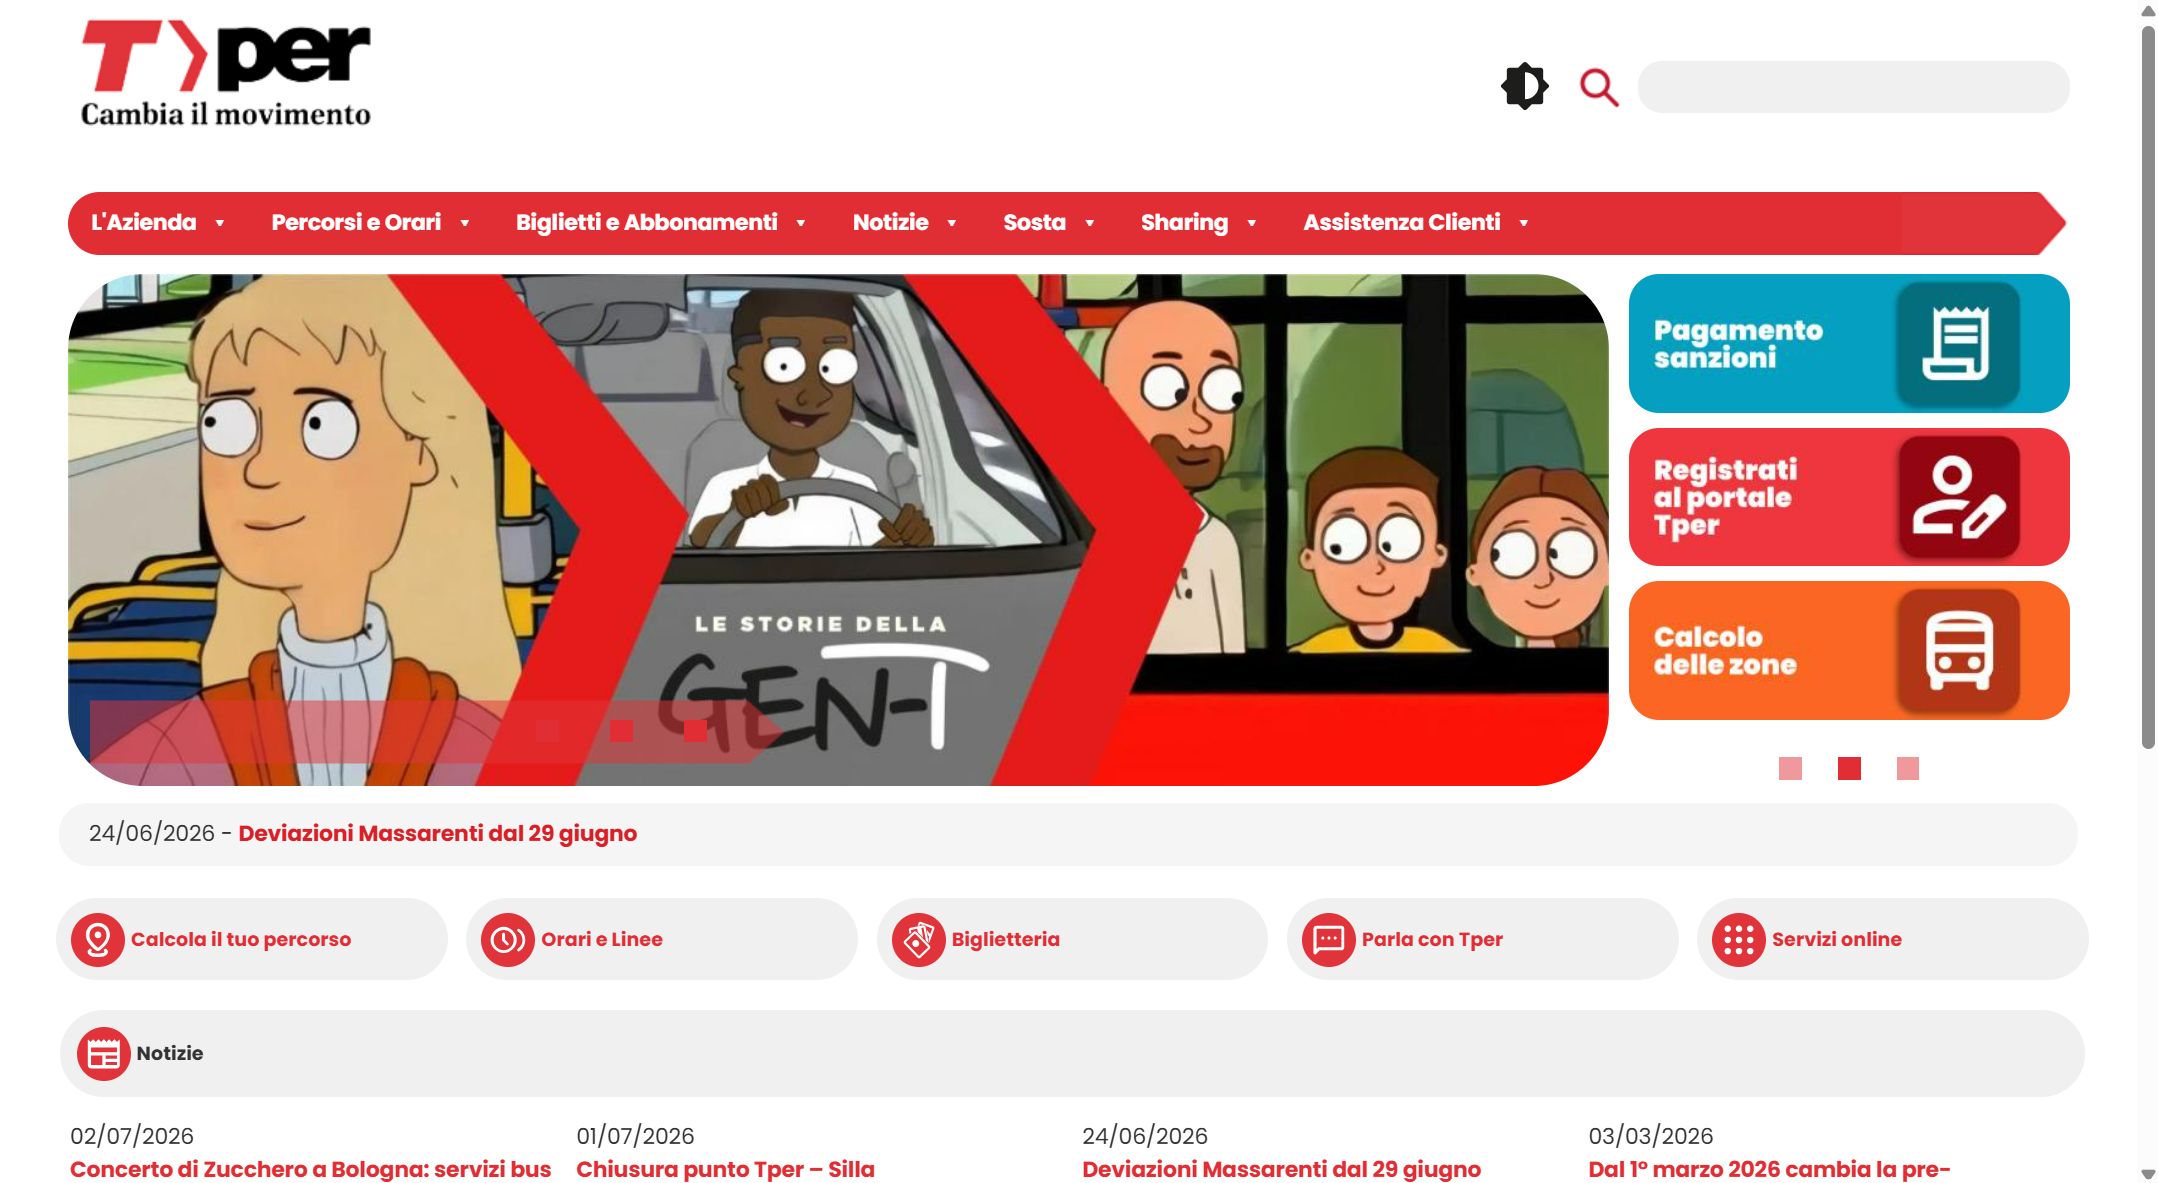
\includegraphics[width=\textwidth]{Tper sito originale/Homepage.png}
\par\small\textit{Before: \texttt{tper.it} live --- slider di news aziendali, nessuna CTA primaria}
\end{minipage}
\hfill
\begin{minipage}[t]{0.498\textwidth}
\centering
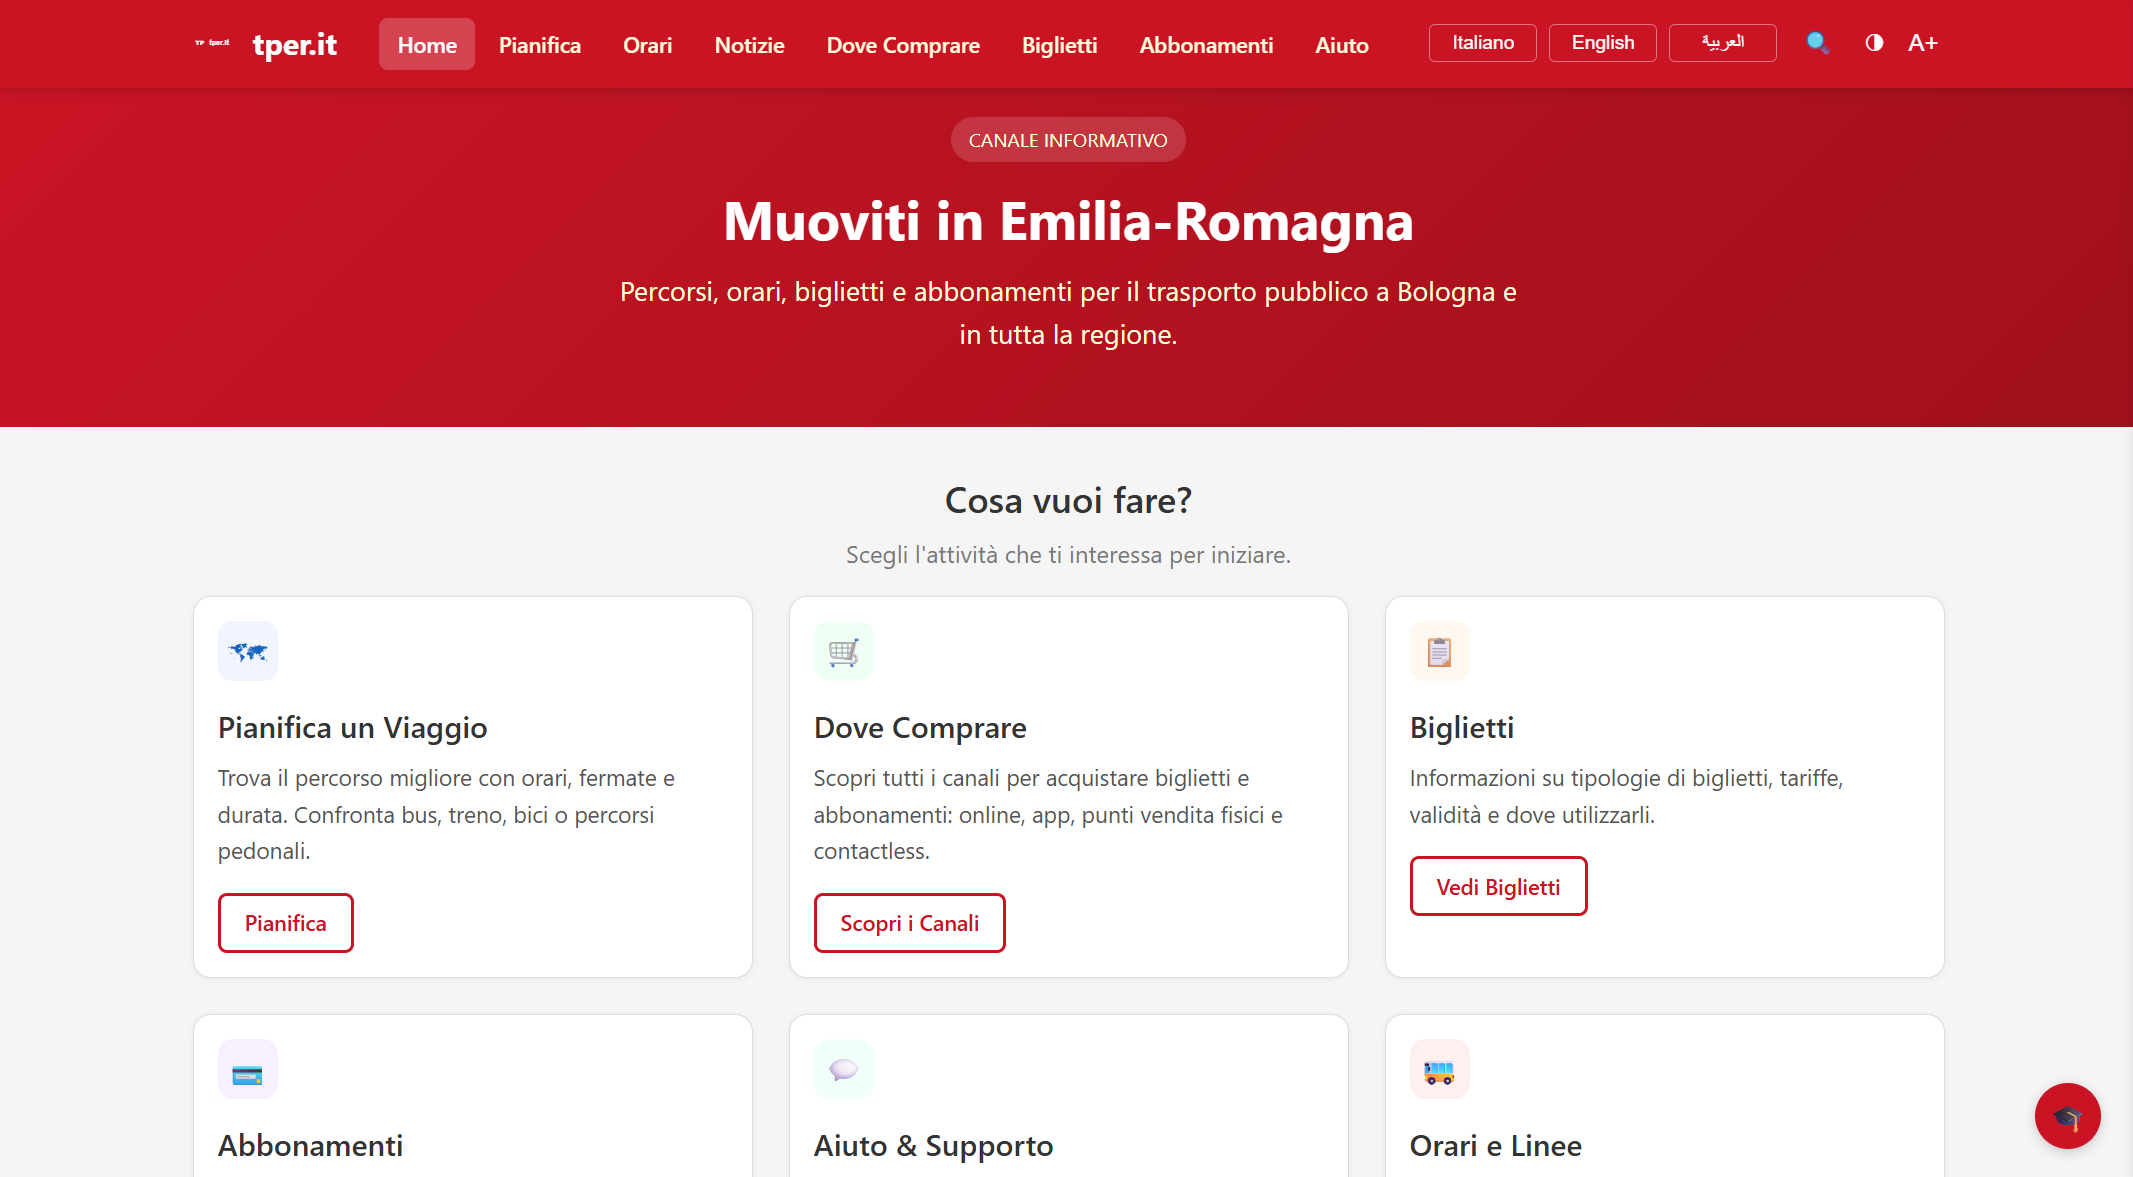
\includegraphics[width=\textwidth]{Redesign Tper 2.0/homepage.png}
\par\small\textit{After: tper 2.0 --- hero pianificatore + griglia 6 card task-oriented}
\end{minipage}
\caption{Homepage \texttt{tper.it}}
\label{fig:comparison-home}
\end{figure}

\begin{table}[H]
\centering
\small
\renewcommand{\arraystretch}{1.4}
\begin{tabular}{|p{0.5cm}|p{7cm}|p{7cm}|}
\hline
& \textbf{Before} & \textbf{After} \\ \hline
\cellcolor{primaryColor!15} &
\textit{Homepage attuale di \texttt{tper.it} (live)} &
\textit{Homepage redesign \texttt{tper 2.0}} \\ \hline

\raisebox{0.5cm}{\rotatebox{90}{\textbf{Contenuti}}} &
Slider di notizie aziendali, comunicati stampa, bandi di gara occupano la homepage. Il pianificatore di viaggio è raggiungibile dopo 2--3 click attraverso \textit{Percorsi e Orari} $\rightarrow$ \textit{Calcola il tuo percorso}. Nessuna gerarchia tra contenuti utente e contenuti istituzionali (Issue D1). &
Hero section dedicata al pianificatore di viaggio con campi ``Partenza'' e ``Destinazione'' già visibili. Griglia ``Cosa vuoi fare?'' con 6 card task-oriented: Pianifica, Dove Comprare, Biglietti, Abbonamenti, Aiuto, Orari. News aziendali spostate in sezione separata (R1). \\ \hline

\raisebox{0.5cm}{\rotatebox{90}{\textbf{CTA}}} &
Link testuali generici: ``Servizi online'', ``Percorsi e Orari'', ``Biglietteria'', ``Parla con Tper''. L'utente deve interpretare la terminologia aziendale per capire dove andare (Issue D3). &
Pulsanti grandi con icone e linguaggio utente: ``Pianifica un Viaggio'', ``Dove Comprare?'', ``Vedi Biglietti'', ``Scopri Abbonamenti'', ``Vai all'Aiuto'', ``Consulta Orari''. Ogni card mostra un'icona distintiva colorata (R2, R9). \\ \hline

\raisebox{0.5cm}{\rotatebox{90}{\textbf{Navigazione}}} &
Mega-menu con 7 voci principali e oltre 50 sottovoci, dominato da contenuti istituzionali: \textit{Società Trasparente}, \textit{Appalti e Fornitori}, \textit{L'Azienda} occupano la maggior parte dello spazio. L'utente si perde tra contenuti legali (Issue D2). &
Navigazione flat a 8 voci task-oriented: Home, Pianifica, Orari, Notizie, \textbf{Dove Comprare}, Biglietti, Abbonamenti, Aiuto. Breadcrumb su tutte le pagine interne per orientamento. Contenuti istituzionali disponibili via footer (R2, R3). \\ \hline

\raisebox{0.5cm}{\rotatebox{90}{\textbf{Info}}} &
Nessuna indicazione sul ruolo informativo del sito. L'utente cerca funzioni transazionali che non esistono su \texttt{tper.it} (UR-01, UR-03). &
Banner esplicito su ogni pagina: ``\texttt{tper.it} è un sito informativo. Per acquistare biglietti e abbonamenti utilizza uno dei canali dedicati'' con link a Dove Comprare. Hero badge: ``CANALE INFORMATIVO'' (R1). \\ \hline
\end{tabular}
\caption{Homepage (\texttt{tper.it} live vs tper 2.0)}
\label{tab:comparison-home}
\end{table}

\vspace{0.3cm}

% ============================================================
% CONFRONTO 2: HOMEPAGE solweb
% ============================================================
\section{Home Page \texttt{solweb.tper.it}}
\label{sec:comparison-solweb-home}

\textbf{D5 $\rightarrow$ R7} --- Login obbligatorio (P3,I5) $\rightarrow$ Guest path + 4 azioni rapide. 3/4 falliti T3, transizione \texttt{tper.it}$\rightarrow$\texttt{solweb} non segnalata.

\begin{figure}[H]
\centering
\begin{minipage}[t]{0.498\textwidth}
\centering
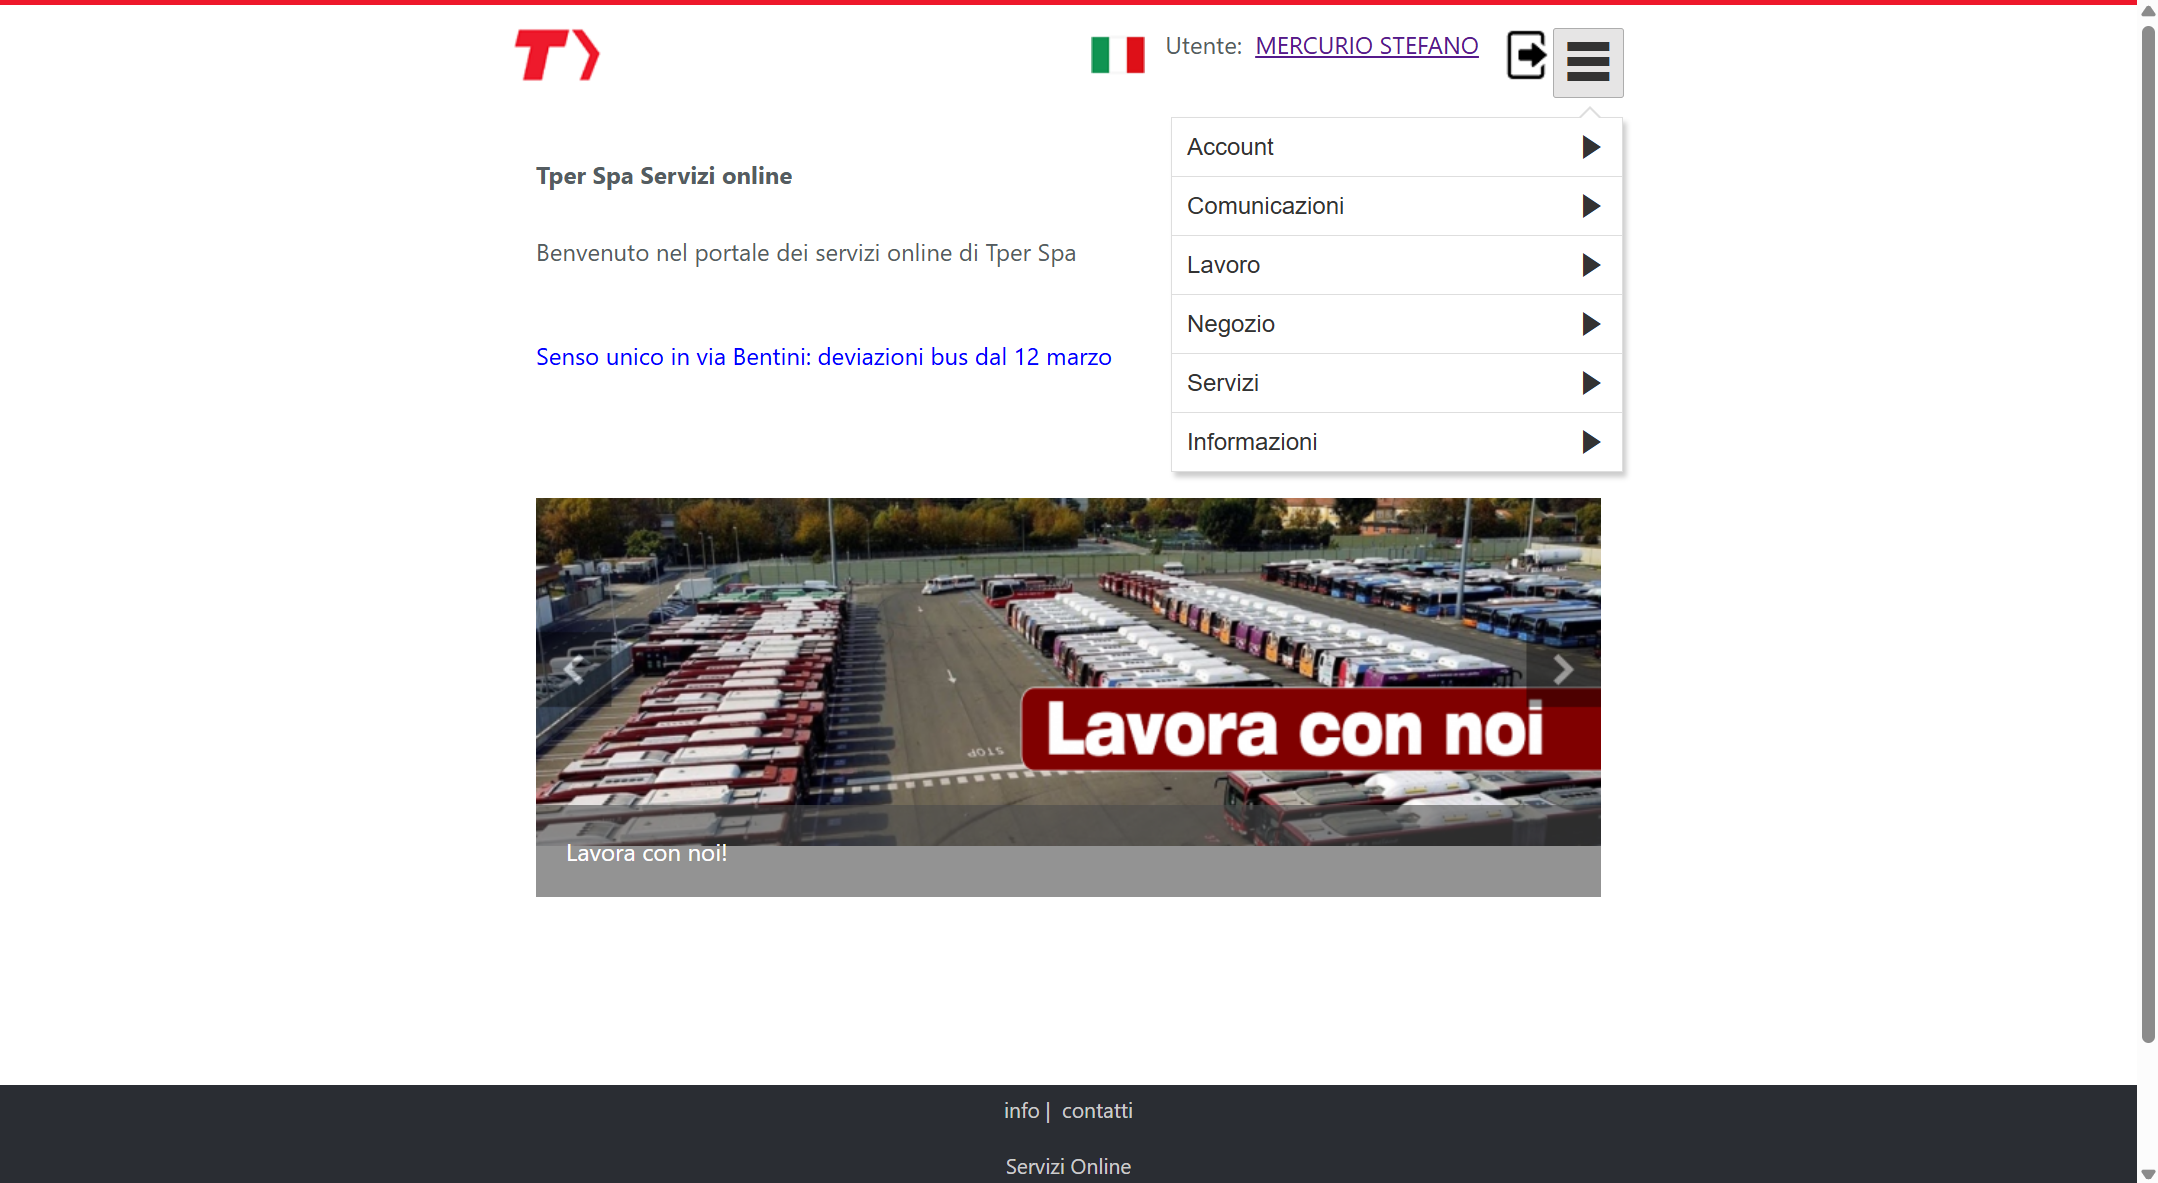
\includegraphics[width=\textwidth]{Tper sito originale/HomepageS.png}\\[2pt]
{\small\textit{+ seconda vista:}}\\[2pt]
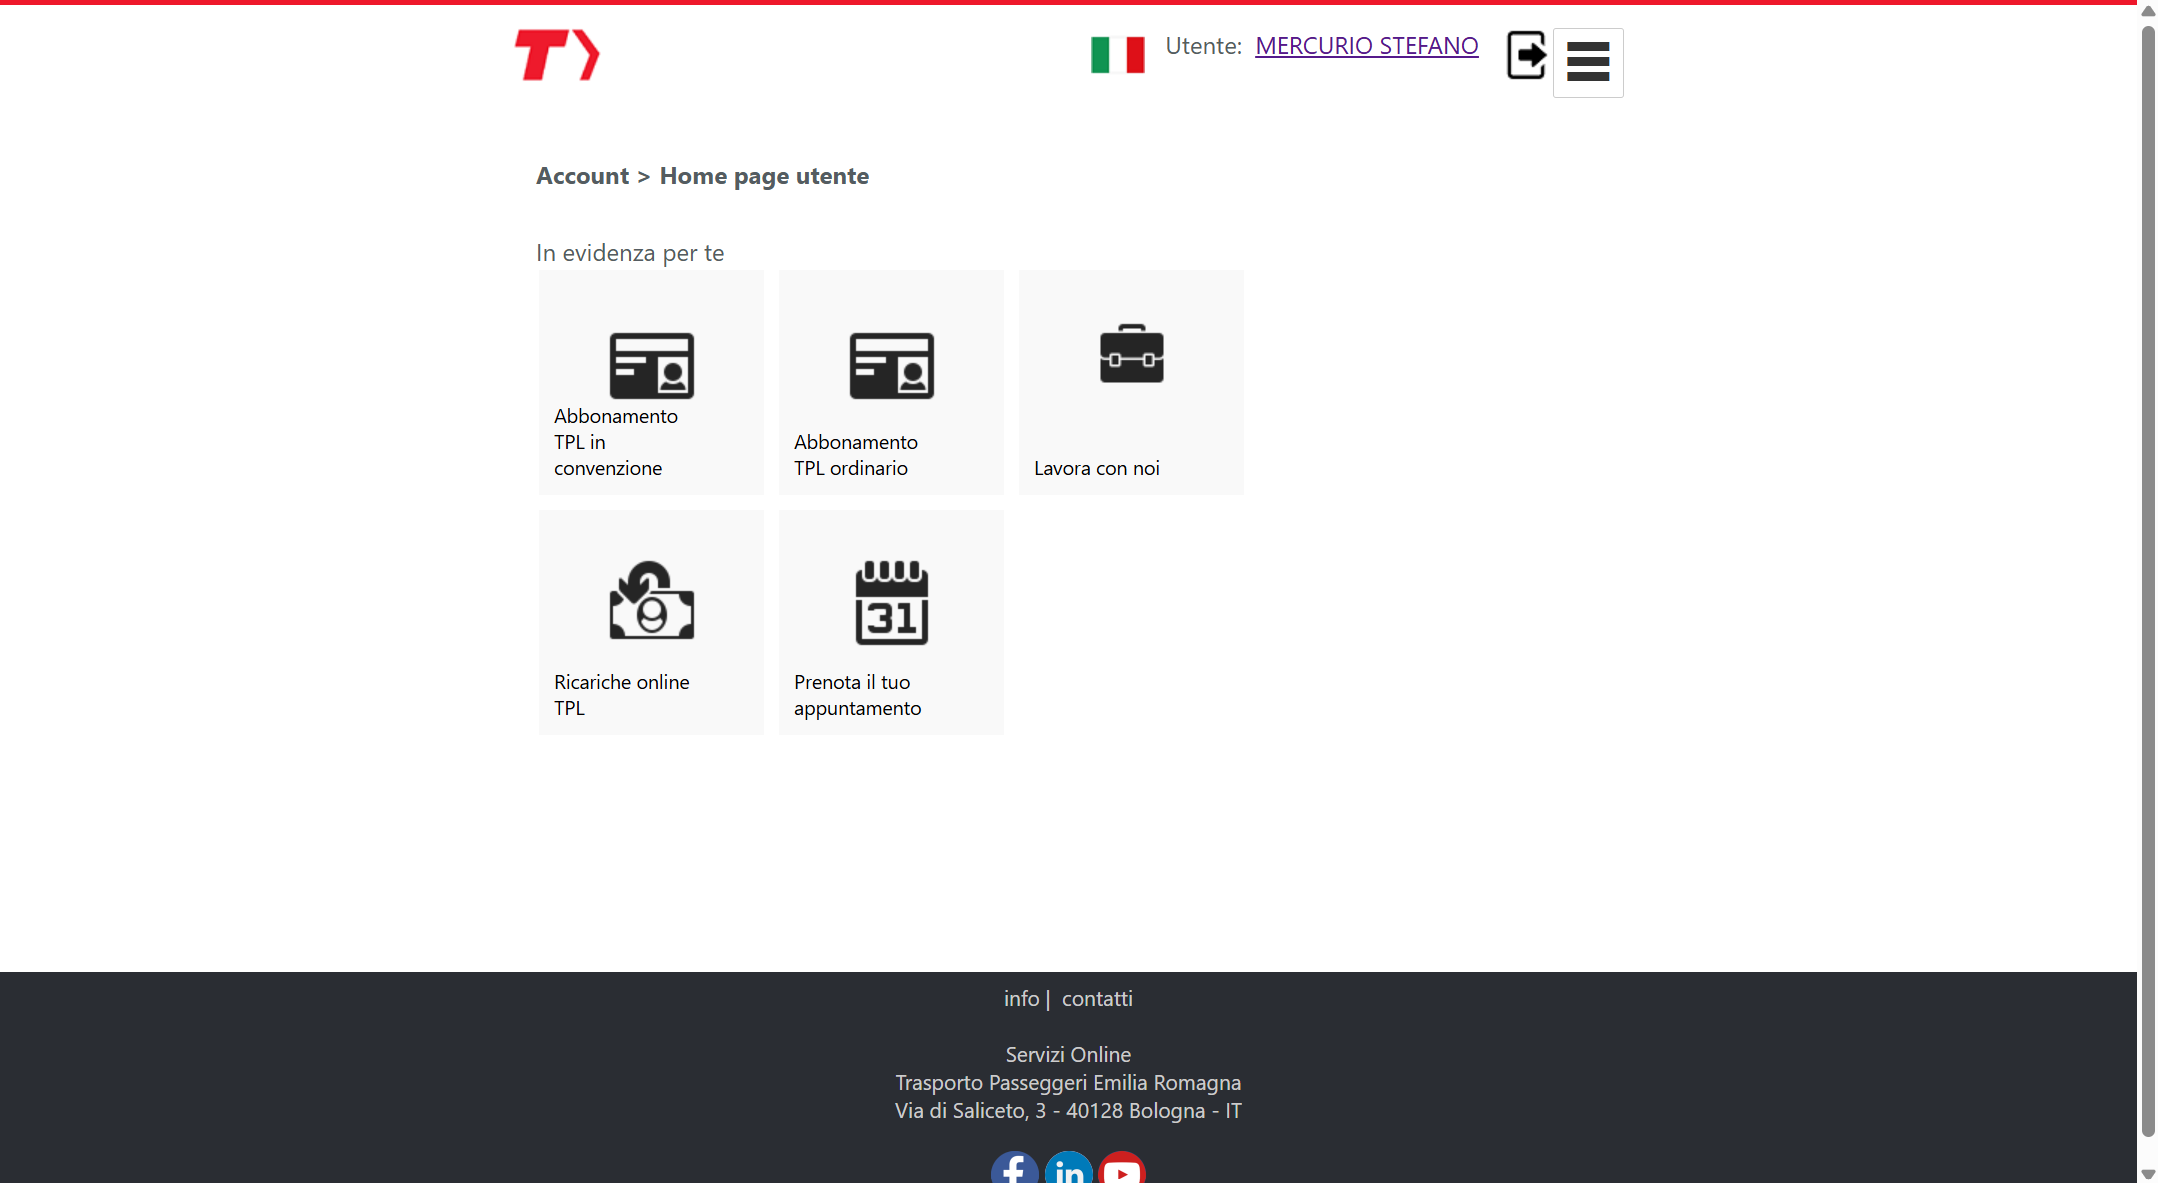
\includegraphics[width=\textwidth]{Tper sito originale/HomepageS2.png}
\par\small\textit{Before: \texttt{solweb} originale --- login obbligatorio, nessun percorso guest}
\end{minipage}
\hfill
\begin{minipage}[t]{0.498\textwidth}
\centering
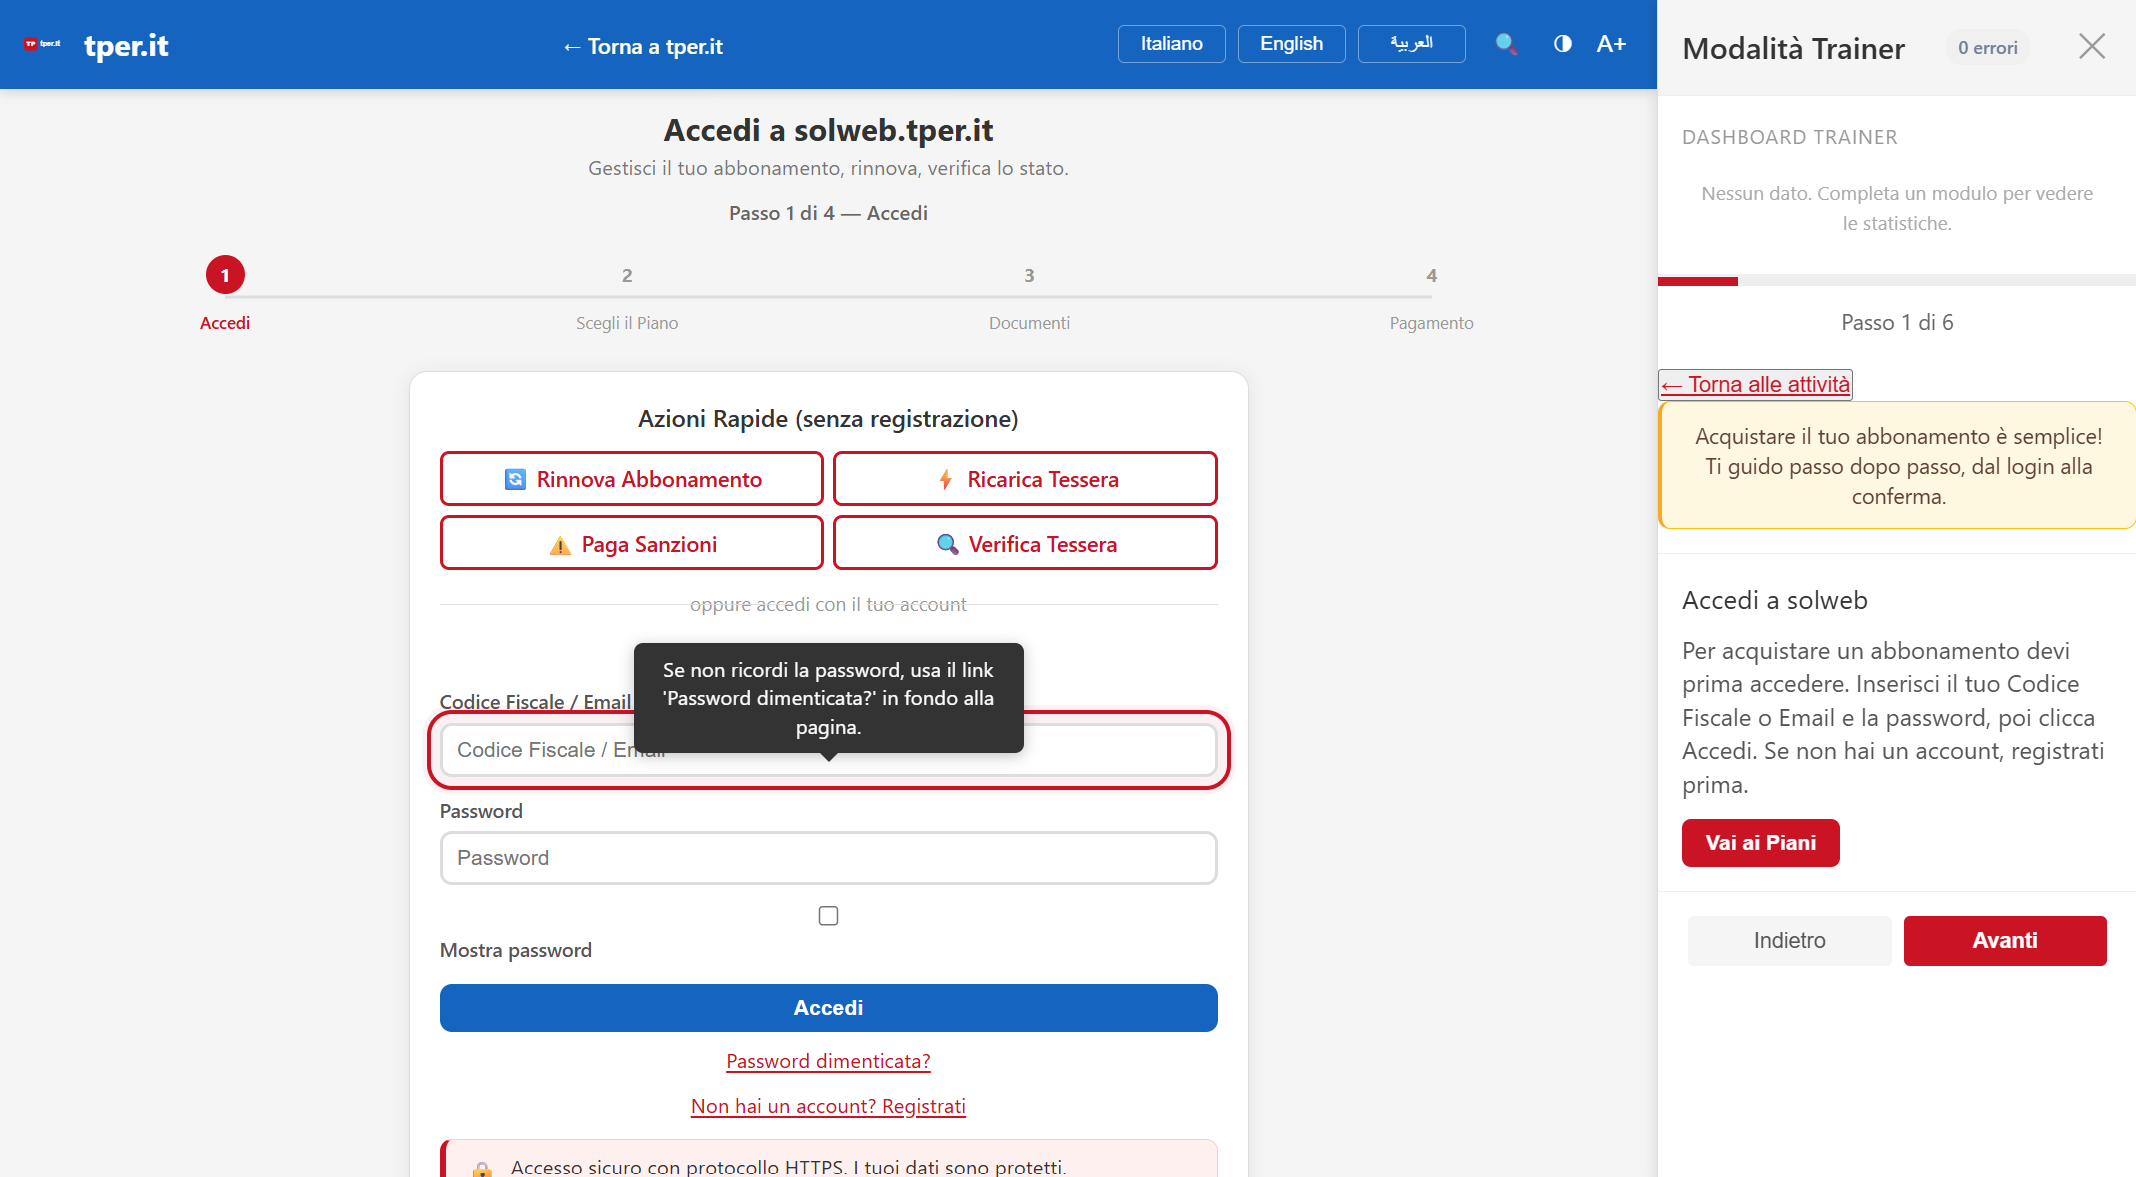
\includegraphics[width=\textwidth]{Redesign Tper 2.0/HomepageS.png}
\par\small\textit{After: solweb 2.0 --- login + 4 azioni rapide senza registrazione}
\end{minipage}
\caption{Homepage \texttt{solweb.tper.it}}
\label{fig:comparison-solweb-home}
\end{figure}

\begin{table}[H]
\centering
\small
\renewcommand{\arraystretch}{1.4}
\begin{tabular}{|p{0.5cm}|p{7cm}|p{7cm}|}
\hline
& \textbf{Before} & \textbf{After} \\ \hline
\cellcolor{primaryColor!15} &
\textit{Portale solweb originale} &
\textit{solweb 2.0 nel redesign} \\ \hline

\raisebox{0.5cm}{\rotatebox{90}{\textbf{Accesso}}} &
\textbf{Solo login}: username/SPID/CIE obbligatori per qualsiasi operazione. Nessuna alternativa guest. Per un utente anziano a bassa competenza digitale, la richiesta di ``creare un account'' causa abbandono immediato (Issue D5). &
\textbf{4 azioni rapide senza login}: Rinnovo Impersonale, Ricarica Tessera, Paga Sanzioni, Verifica Tessera. Il login resta disponibile per le operazioni che richiedono autenticazione (ISEE, abbonamenti personali). Barra di progresso a 4 passi: Accedi $\rightarrow$ Scegli il Piano $\rightarrow$ Documenti $\rightarrow$ Pagamento (R7). \\ \hline

\raisebox{0.5cm}{\rotatebox{90}{\textbf{Transizione}}} &
Passaggio da \texttt{tper.it} a \texttt{solweb} senza alcun avviso: cambio di dominio, interfaccia, colori e layout. L'utente non capisce se è ancora su TPER (Issue R4). &
\textbf{Modale di transizione} prima di ogni link esterno: ``Stai per uscire da \texttt{tper.it} --- Verrai reindirizzato al canale di acquisto esterno'' con URL di destinazione visibile (R9). Header solweb con link ``$\leftarrow$ Torna a tper.it'' sempre visibile. \\ \hline

\raisebox{0.5cm}{\rotatebox{90}{\textbf{Orientamento}}} &
Nessuna indicazione di dove ci si trova nell'ecosistema. Interfaccia completamente diversa da \texttt{tper.it}, zero segnaletica di continuità. &
Header blu (\#1565C0) distinto dal rosso TPER per segnalare il cambio di piattaforma. Hero badge ``PIATTAFORMA ABBONAMENTI'' nella dashboard. Breadcrumb contestuali. \\ \hline

\raisebox{0.5cm}{\rotatebox{90}{\textbf{Operazioni}}} &
Tutte le operazioni richiedono registrazione. Nessuna distinzione tra operazioni semplici (ricarica, sanzioni) e complesse (ISEE, rinnovo personale). &
\textbf{Separazione guest/authenticated}: ricarica, sanzioni e verifica tessera accessibili senza login. Acquisto e rinnovo personale protetti da autenticazione con spiegazione del perché (R7). \\ \hline
\end{tabular}
\caption{Homepage \texttt{solweb.tper.it}}
\label{tab:comparison-solweb-home}
\end{table}

\vspace{0.3cm}

% ============================================================
% CONFRONTO 3: RISTRUTTURAZIONE IA (3v3)
% ============================================================
\section{Ristrutturazione dell'Architettura Informativa}
\label{sec:comparison-ia-3v3}

\textbf{D2+D3 $\rightarrow$ R2+R9} --- Menu 200+ voci, 5 livelli $\rightarrow$ Nav piatta 8 voci. ``Rete di vendita'' sepolta al 3° livello.

\subsection*{Il Problema Originale}

Nel sito originale, tre pagine si sovrapponevano generando confusione e duplicazione:

\begin{itemize}[nosep]
    \item \textbf{Biglietti}: elencava biglietti + canali di vendita + tariffe --- troppe informazioni per una pagina sola;
    \item \textbf{Abbonamenti}: elencava abbonamenti + canali + tariffe --- stessa duplicazione della pagina Biglietti;
    \item \textbf{Tariffe}: pagina separata con i prezzi, \textbf{ridondante} e scollegata dal contesto d'uso.
\end{itemize}

Risultato: l'utente doveva \textbf{saltare tra 3 pagine} per rispondere a domande come \textit{``quale abbonamento comprare?''} e \textit{``dove lo compro?''}. La guida ai canali (``Rete di vendita'') era sepolta al terzo livello di navigazione.

\subsection*{La Soluzione: Separazione delle Responsabilità}

Il redesign applica il principio \textbf{ogni pagina, un compito} (R2), eliminando ogni duplicazione:

\begin{itemize}[nosep]
    \item \textbf{Biglietti}: \textit{solo} tipologie di biglietto + wizard a 5 domande + filtri per zona/validità/canale;
    \item \textbf{Abbonamenti}: \textit{solo} piani di abbonamento + wizard a 7 domande + verifica agevolazioni;
    \item \textbf{Dove Comprare}: \textbf{nuova sezione dedicata} che raccoglie tutta la guida ai canali --- wizard a 3 domande, 6 card canale, tabella comparativa 5$\times$7.
\end{itemize}

Le \textbf{tariffe} sono state \textbf{integrate} direttamente in Biglietti e Abbonamenti: il prezzo appare nel momento esatto della decisione sul prodotto, non su una pagina separata.

\begin{figure}[H]
\centering
\textbf{Before --- Sito Originale}\\[4pt]
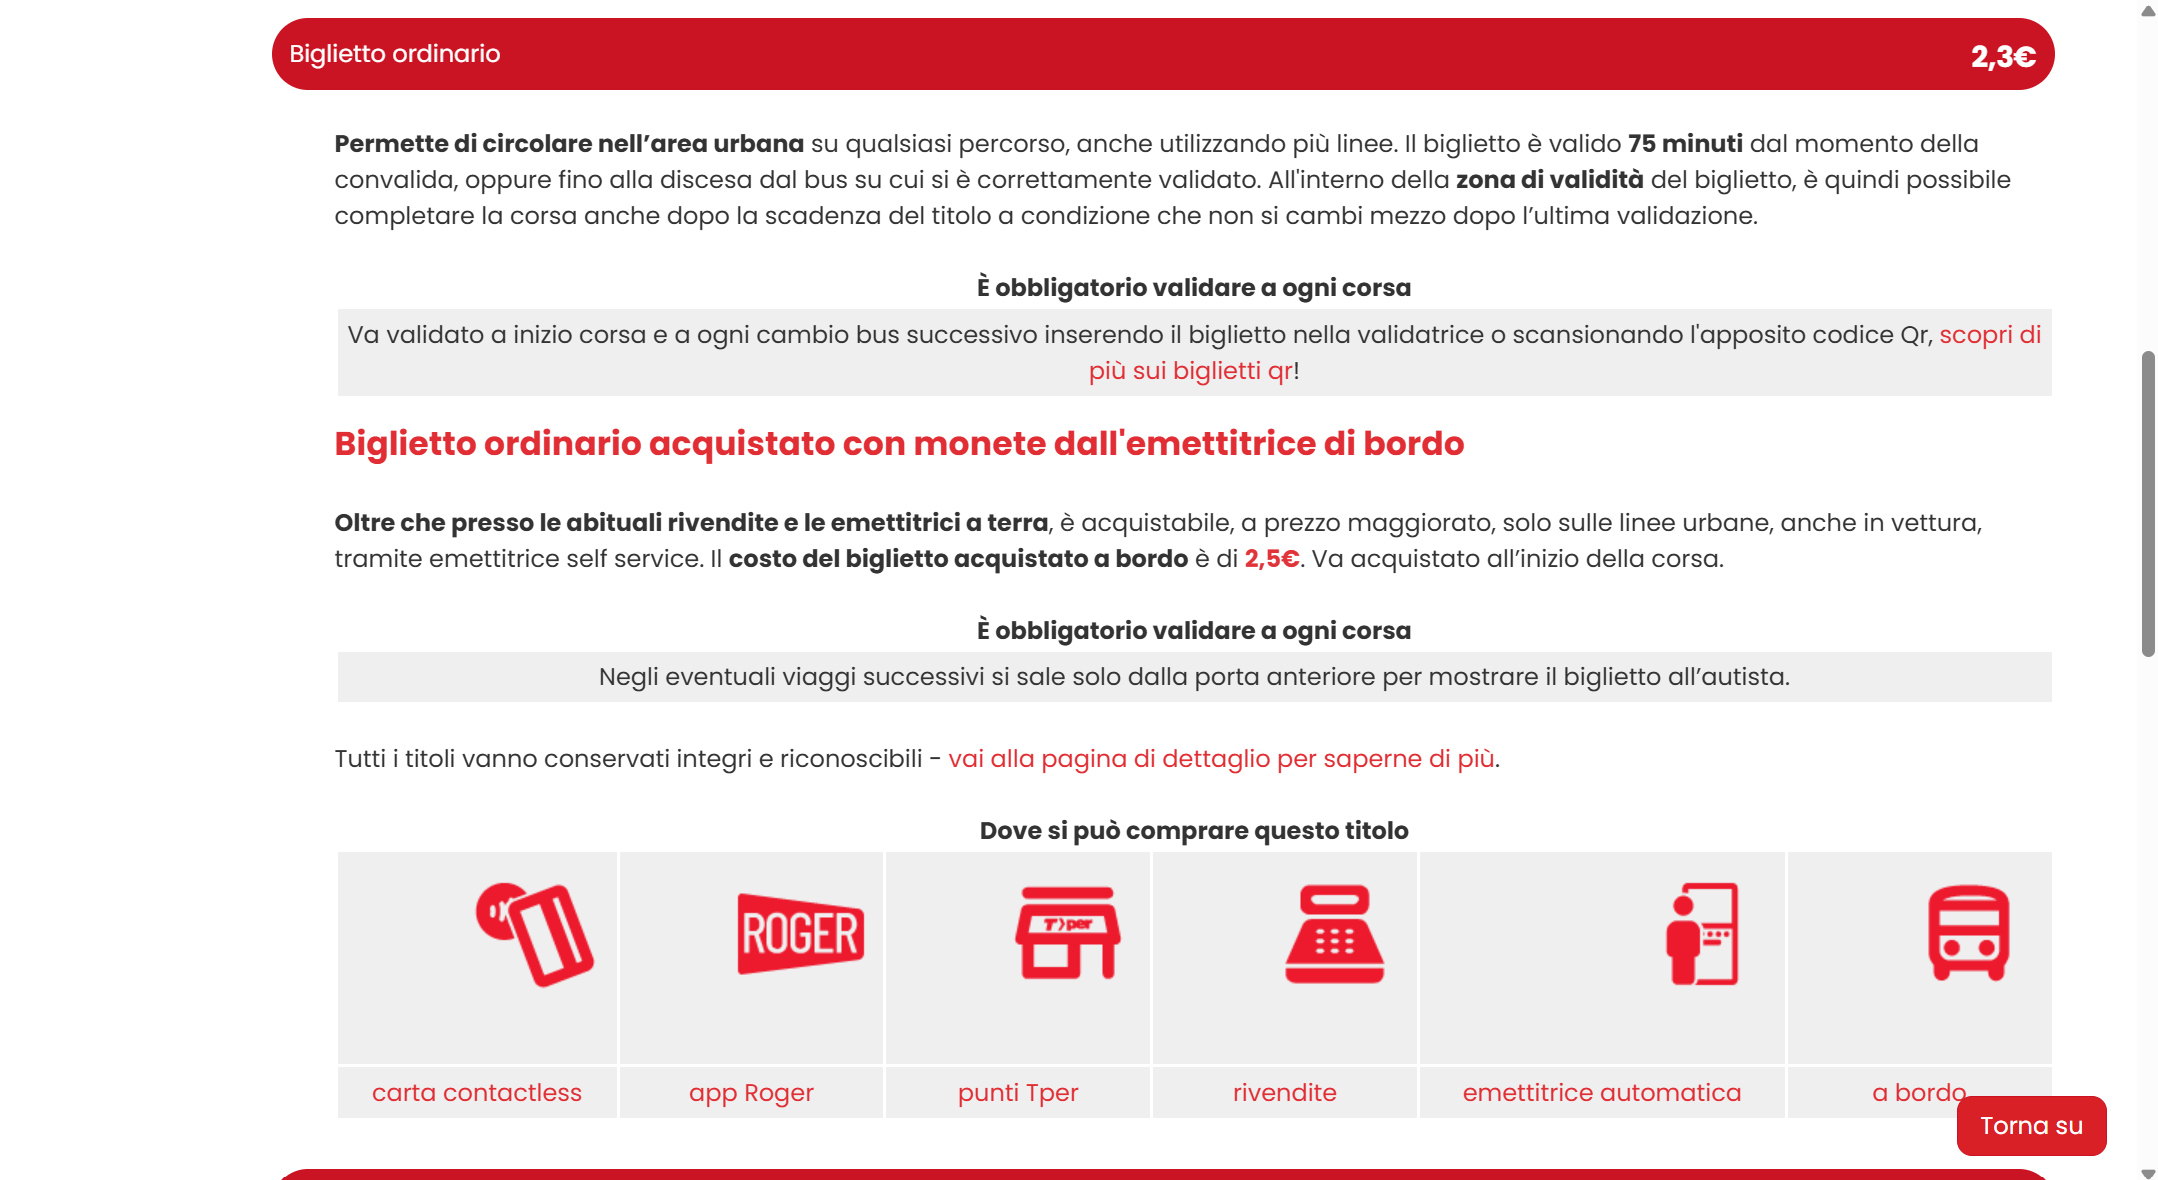
\includegraphics[width=0.332\textwidth]{Tper sito originale/Biglietti.png}\hfill
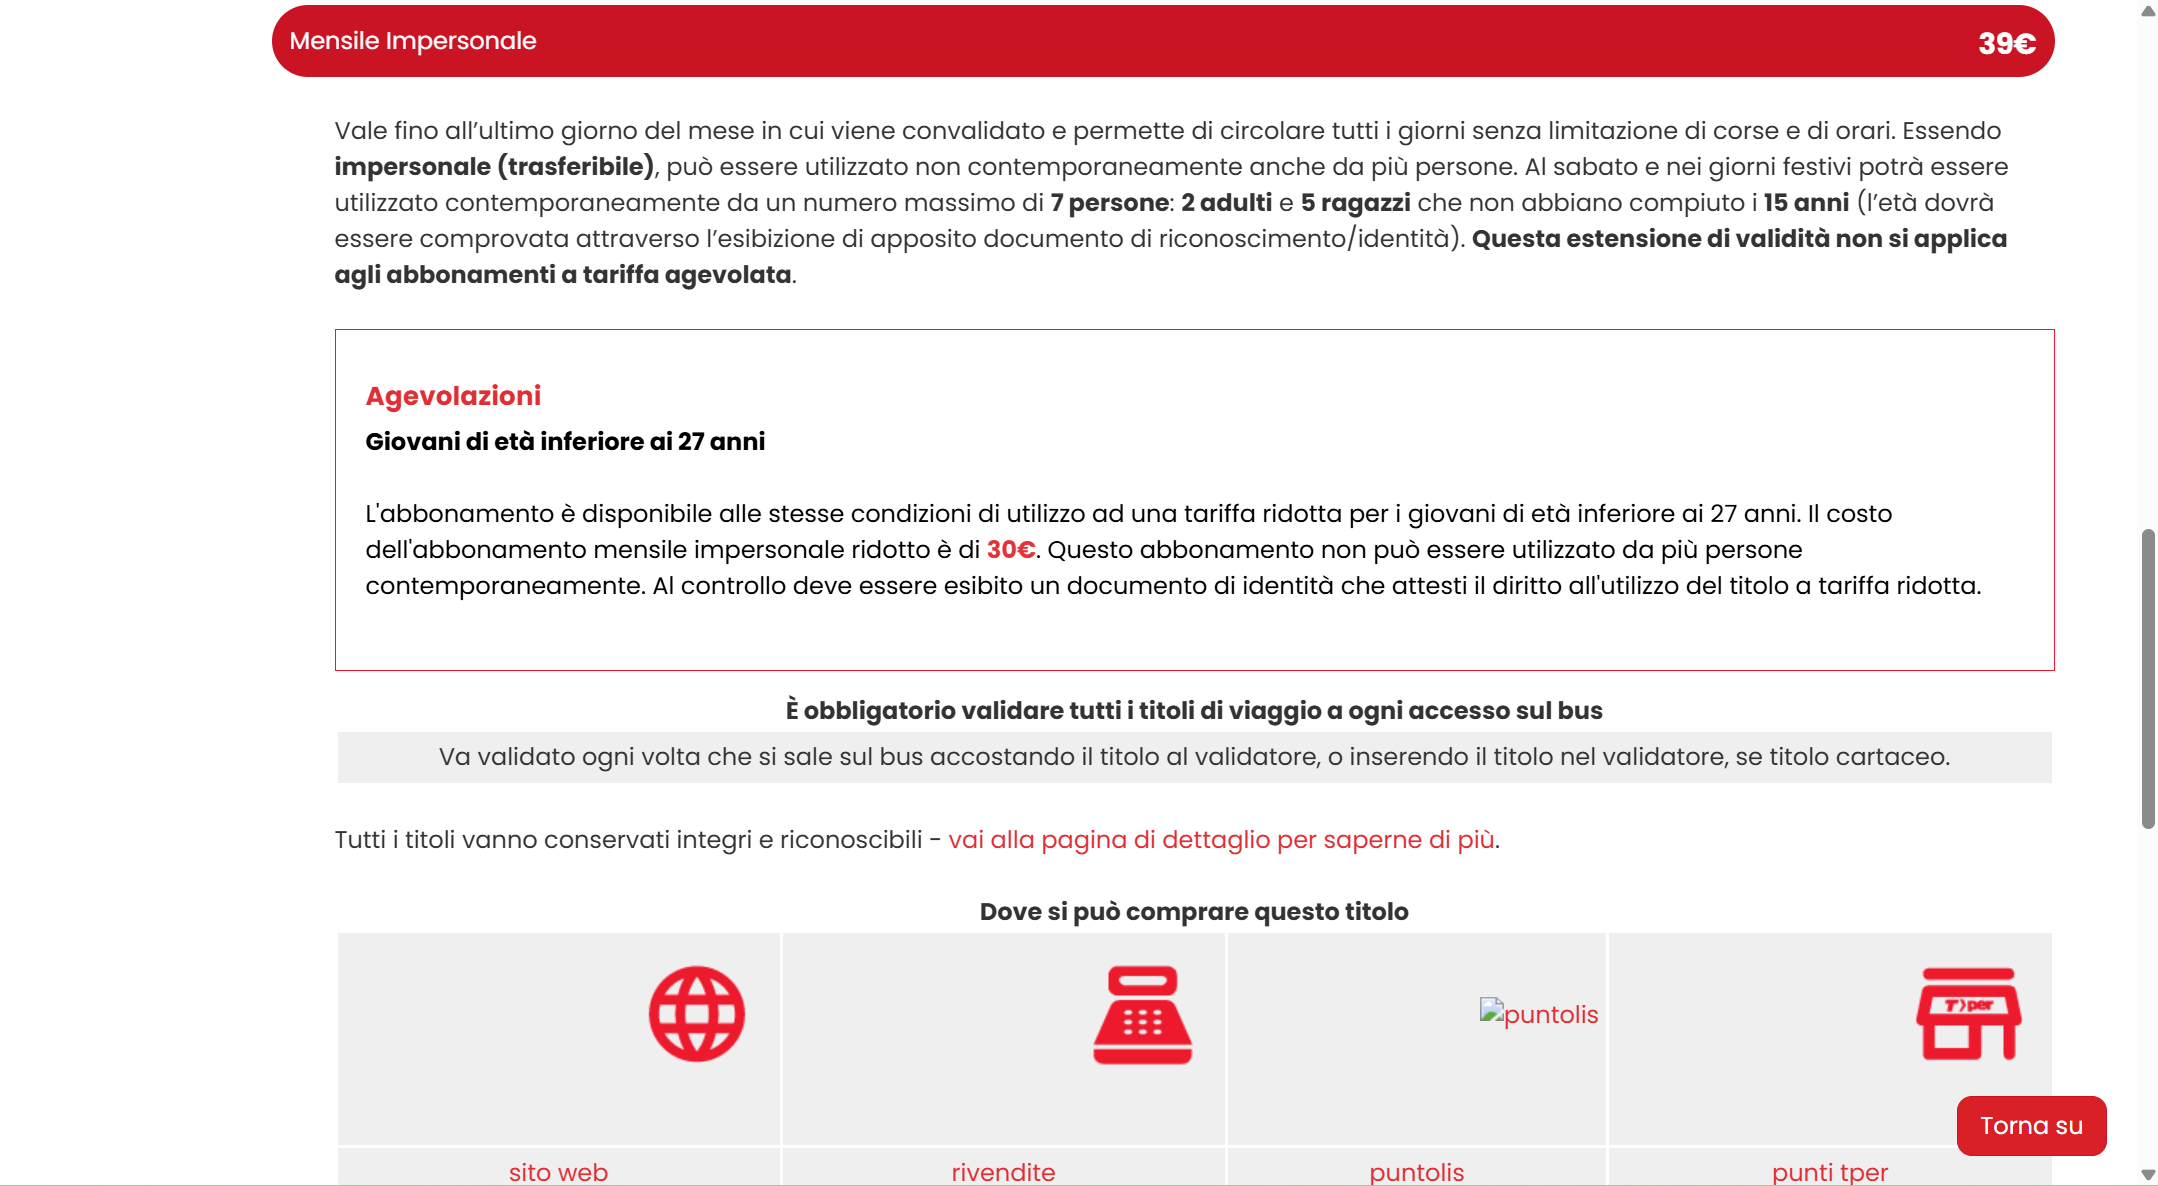
\includegraphics[width=0.332\textwidth]{Tper sito originale/Abbonamenti.png}\hfill
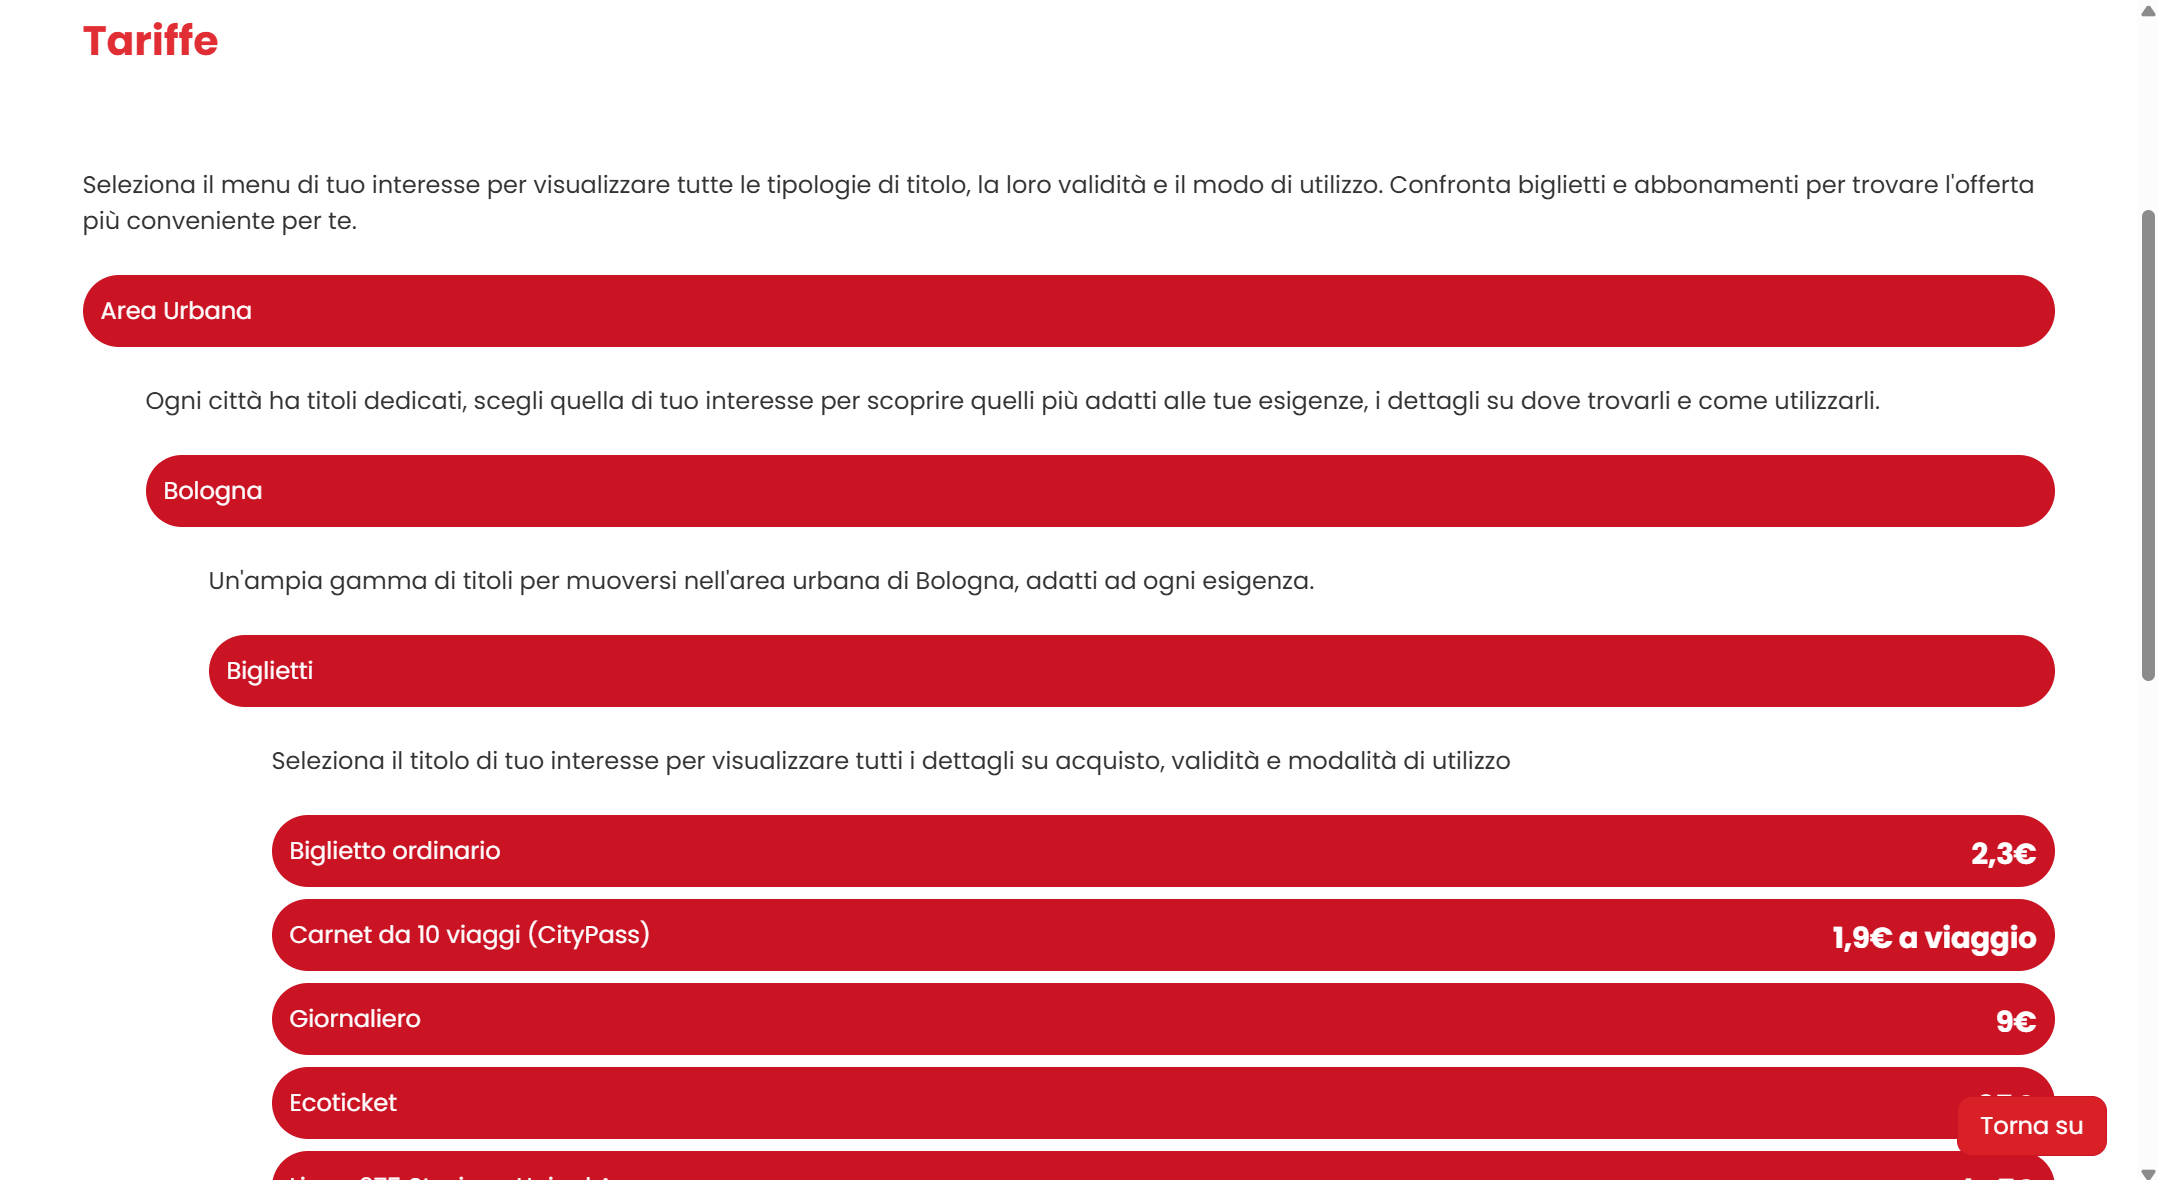
\includegraphics[width=0.332\textwidth]{Tper sito originale/Tariffe.png}\\[2pt]
{\small\textit{Biglietti \hspace{3.3cm} Abbonamenti \hspace{3.3cm} Tariffe}}\\[2pt]
{\footnotesize 3 pagine sovrapposte: contenuti duplicati, canali sepolti, terminologia aziendale}

\vspace{0.5cm}

\textbf{After --- Redesign tper 2.0}\\[4pt]
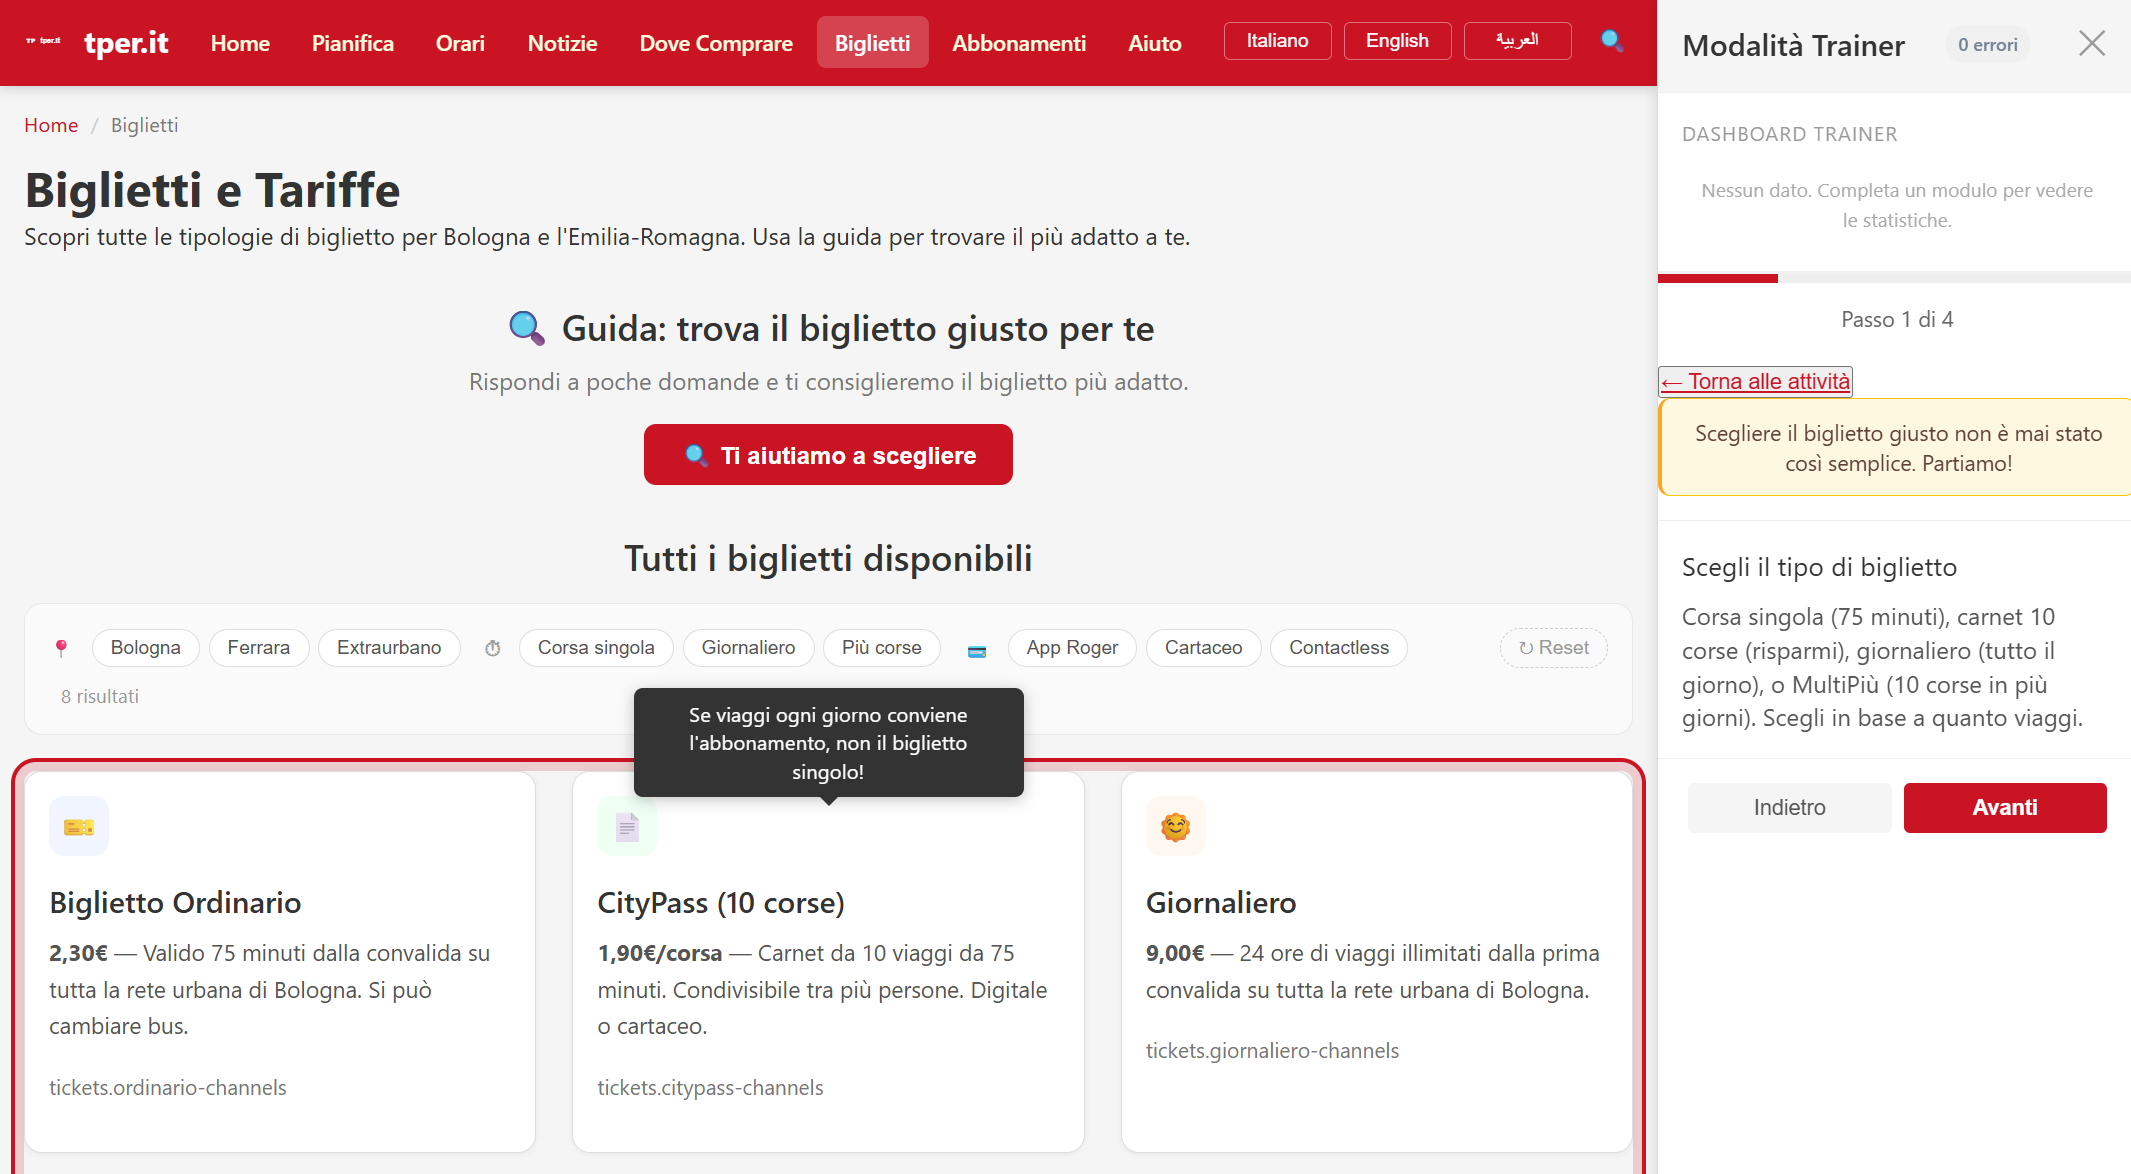
\includegraphics[width=0.332\textwidth]{Redesign Tper 2.0/Biglietti.png}\hfill
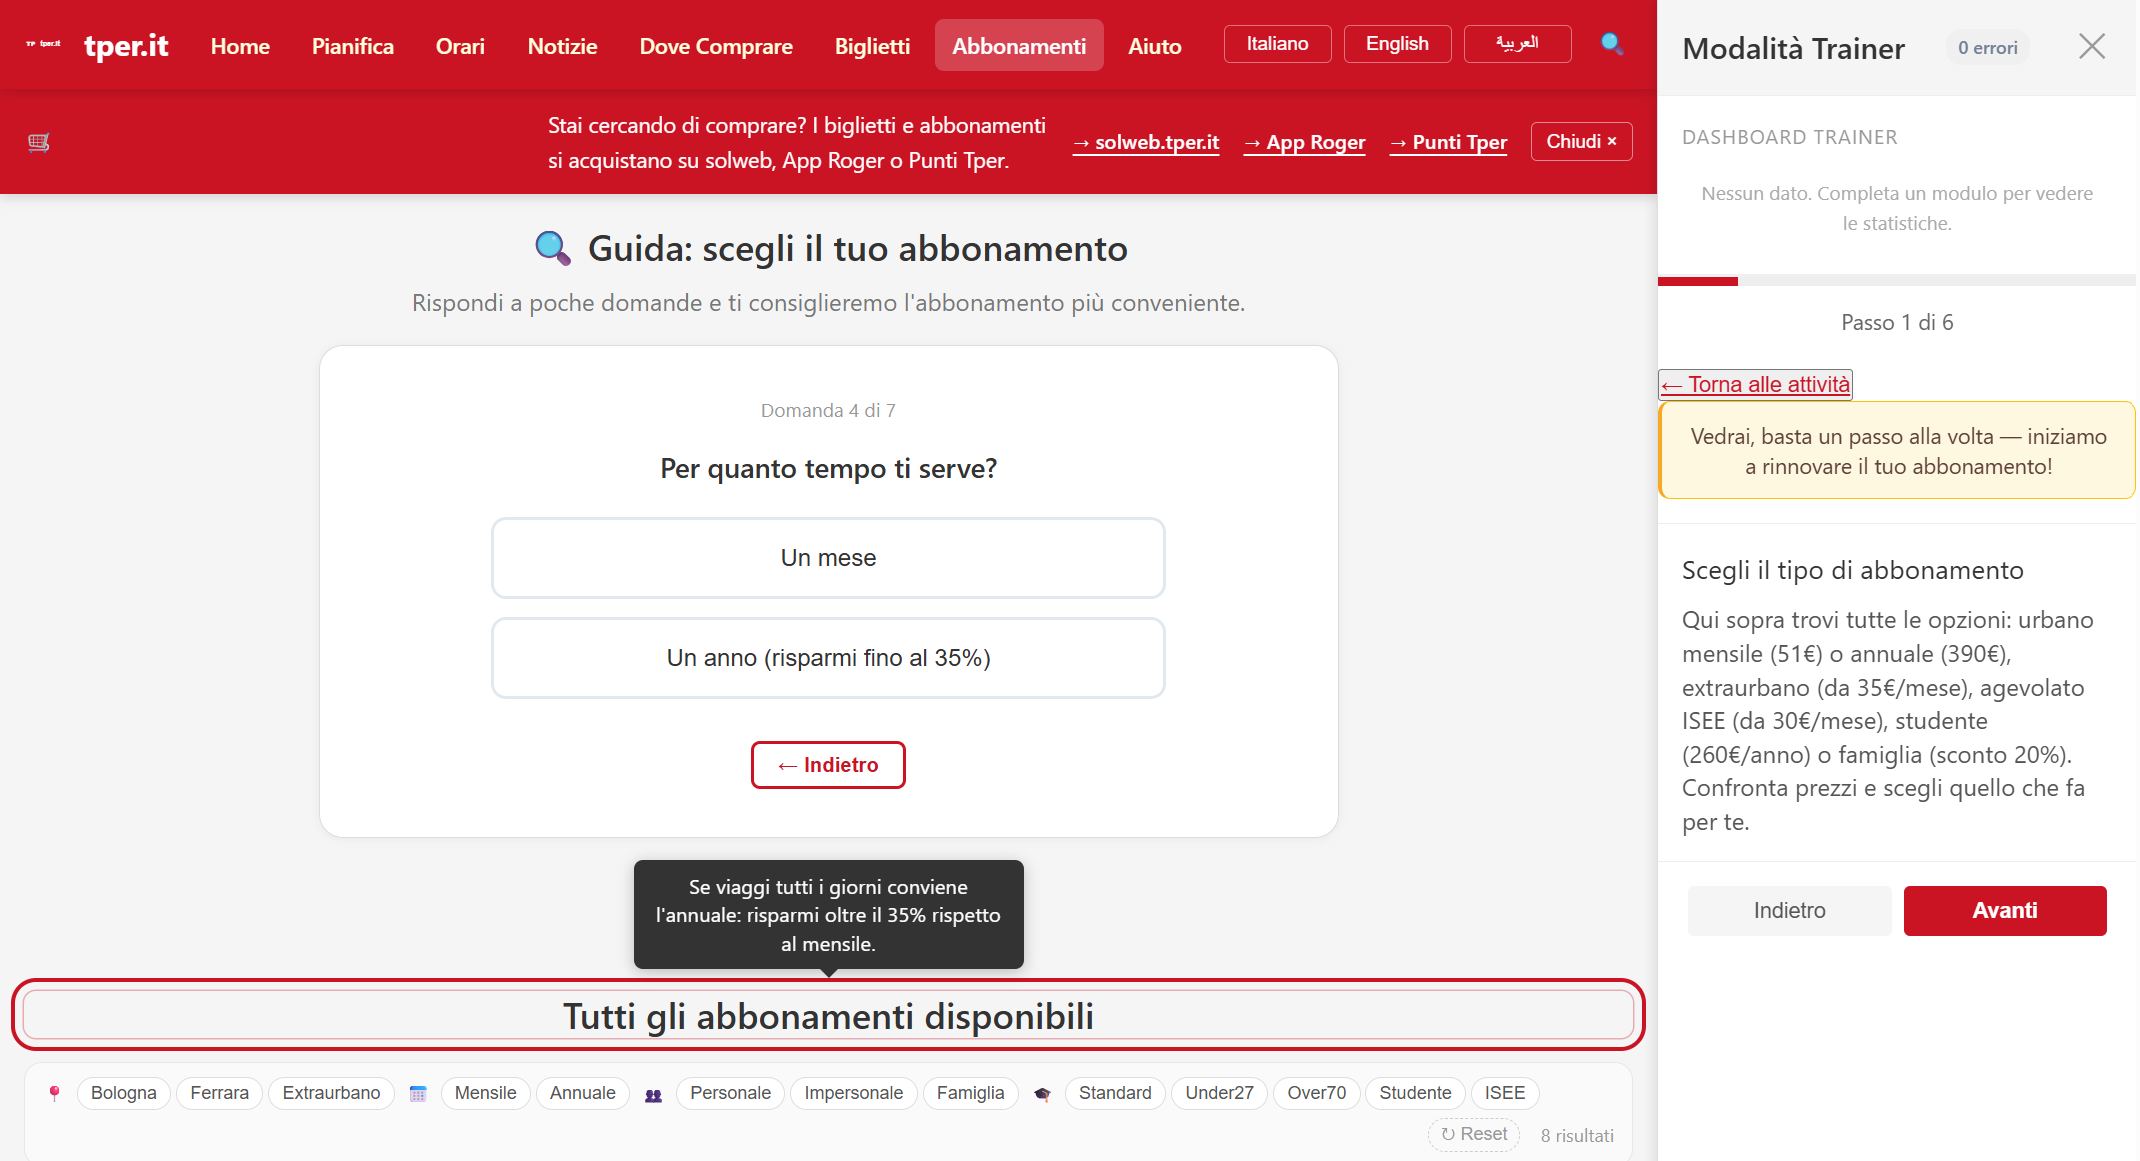
\includegraphics[width=0.332\textwidth]{Redesign Tper 2.0/Abbonamenti.png}\hfill
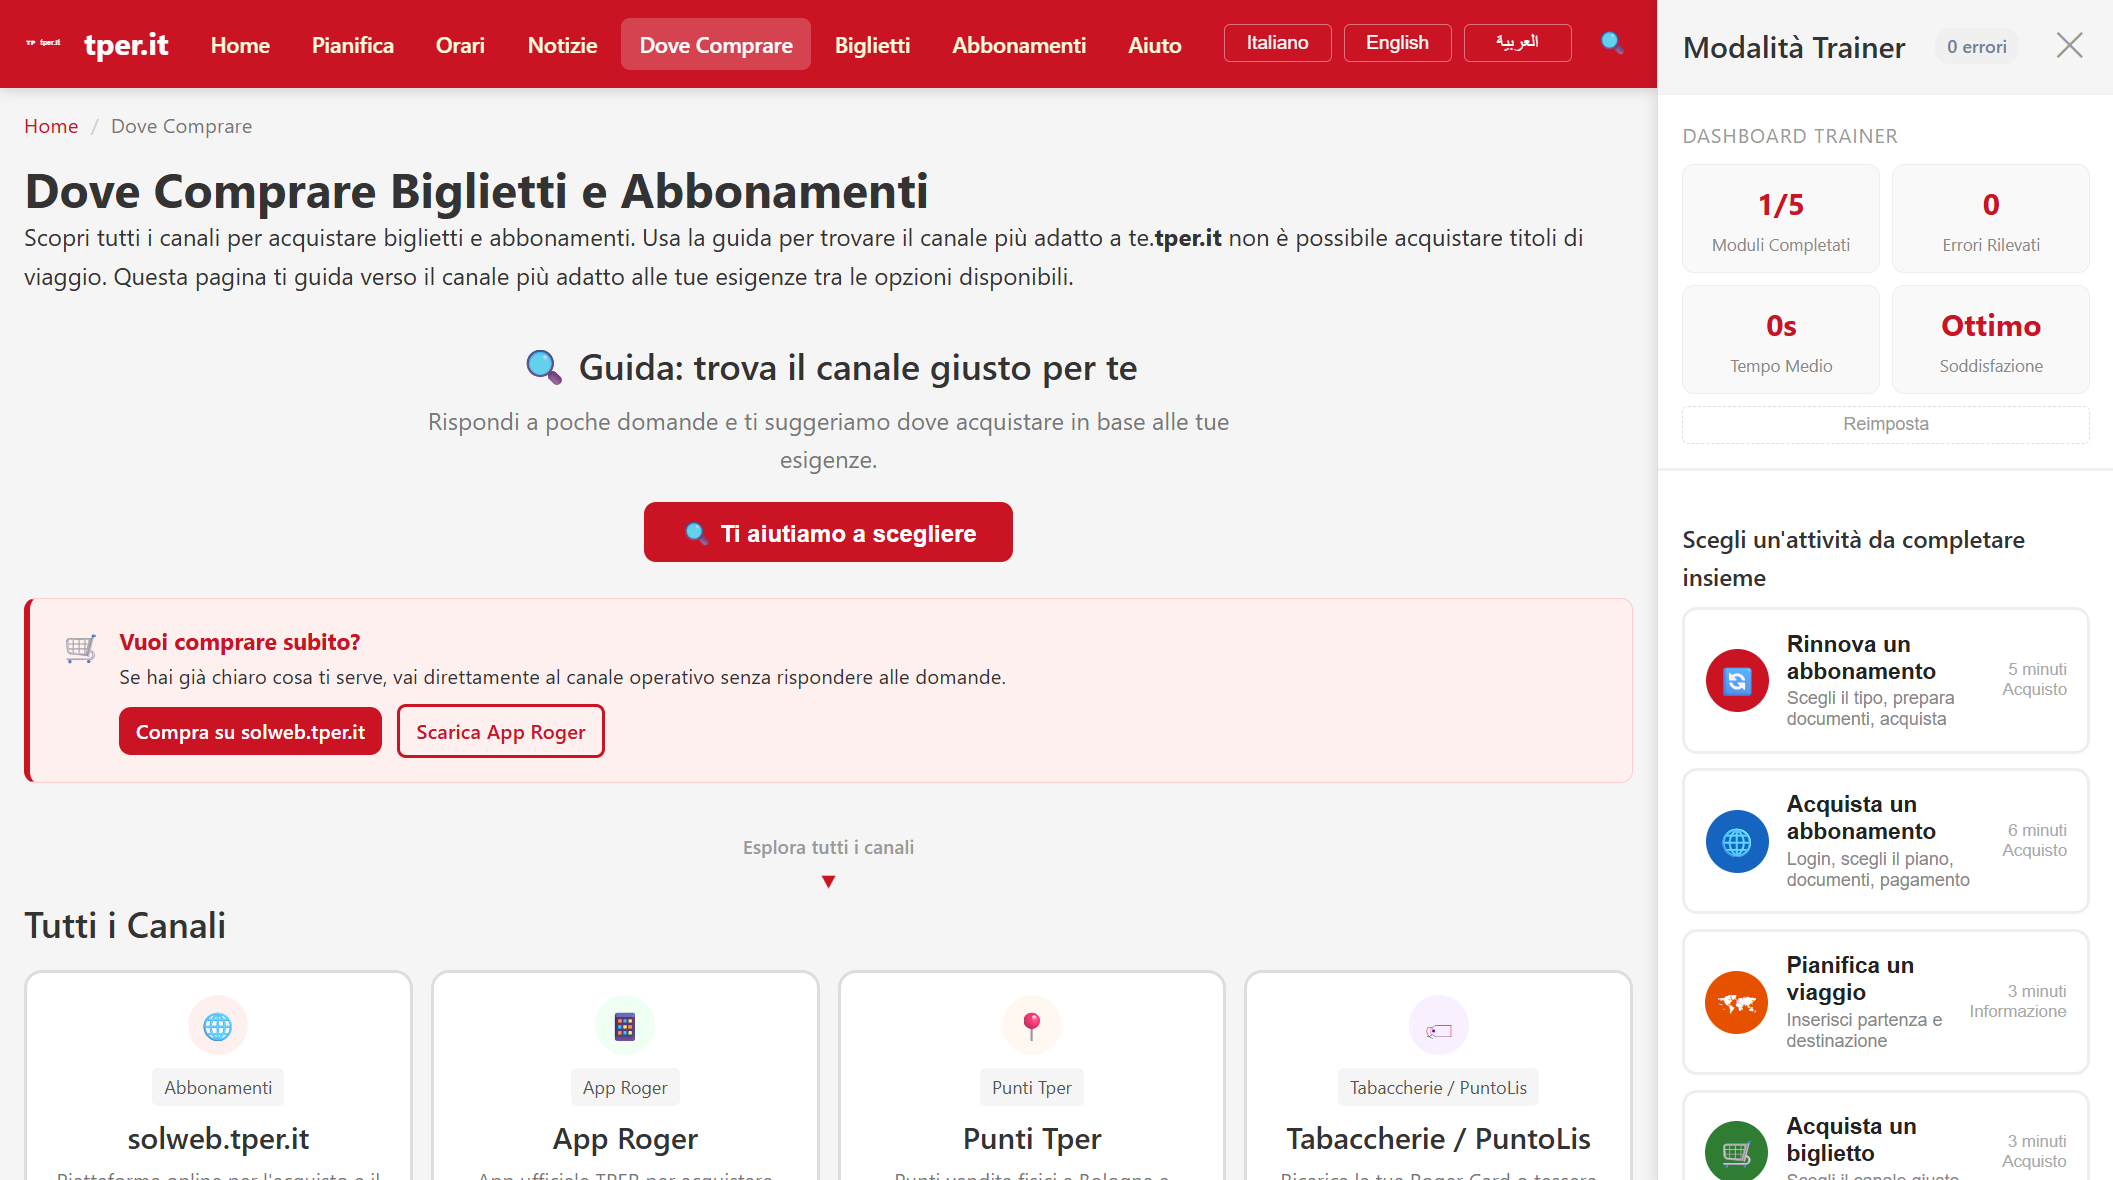
\includegraphics[width=0.332\textwidth]{Redesign Tper 2.0/Dove Comprare.png}\\[2pt]
{\small\textit{Biglietti \hspace{3.3cm} Abbonamenti \hspace{2.8cm} Dove Comprare}}\\[2pt]
{\footnotesize 3 pagine specializzate: ogni pagina ha un compito unico, tariffe integrate nei prodotti}

\caption{Confronto 3v3 --- Ristrutturazione dell'Architettura Informativa}
\label{fig:comparison-ia-3v3}
\end{figure}

\begin{table}[H]
\centering
\small
\renewcommand{\arraystretch}{1.4}
\begin{tabular}{|p{0.5cm}|p{7cm}|p{7cm}|}
\hline
& \textbf{Before (Originale)} & \textbf{After (Redesign 2.0)} \\ \hline
\cellcolor{primaryColor!15} &
\textit{3 pagine sovrapposte} &
\textit{3 pagine specializzate} \\ \hline

\raisebox{0.5cm}{\rotatebox{90}{\textbf{Struttura}}} &
3 pagine con contenuti duplicati e confini sfumati. Biglietti e Abbonamenti contengono entrambi riferimenti a tariffe e canali. La pagina Tariffe è ridondante. Navigazione a 3+ livelli per raggiungere la guida canali (D2). &
3 pagine con responsabilità chiare e distinte. Ogni pagina ha un unico compito. Nessuna duplicazione. Accesso diretto a ogni sezione dalla navigazione principale (max 1 click). Le tariffe sono mostrate nel contesto del prodotto (R2). \\ \hline

\raisebox{0.5cm}{\rotatebox{90}{\textbf{Biglietti}}} &
Elenca tipologie di biglietti, ma include anche informazioni sui canali di vendita e rimandi alle tariffe. L'utente non capisce se questa è la pagina giusta per decidere cosa comprare o dove comprarlo (D2, D3). &
Pagina focalizzata esclusivamente sui biglietti. Wizard a 5 domande (zona, frequenza, durata, app, compagnia). Pillole filtro per zona/validità/canale con contatore e reset. Banner informativo: ``tper.it è un sito informativo''. \\ \hline

\raisebox{0.5cm}{\rotatebox{90}{\textbf{Abbonamenti}}} &
Elenca piani di abbonamento con terminologia aziendale (MiMuovo, SaltaSu, Prontobus). Include canali e tariffe. Nessuna guida alla scelta: l'utente deve leggere tutte le opzioni e dedurre quale fa per lui (UR-05). &
Pagina focalizzata esclusivamente sugli abbonamenti. Wizard a 7 domande (azione, impersonale?, zona, durata, intestatario, agevolazione, canale). Filtro a 4 gruppi. Accordion ``Come Acquistare o Rinnovare''. Callout per verificare diritto a sconto (R9). \\ \hline

\raisebox{0.5cm}{\rotatebox{90}{\textbf{Canali / Tariffe}}} &
\textbf{Canali}: ``Rete di vendita'' sepolta sotto Biglietti e Abbonamenti, raggiungibile in 3 click. \textbf{Tariffe}: pagina separata con prezzi, scollegata dal contesto d'uso --- l'utente deve ricordare il prezzo mentre naviga altrove per decidere (D3). &
\textbf{Dove Comprare}: sezione autonoma e prominente nella navigazione principale. Wizard a 3 domande $\rightarrow$ canale consigliato con icona, descrizione e link diretto. Tabella comparativa 5 canali $\times$ 7 operazioni. \textbf{Tariffe}: integrate in Biglietti e Abbonamenti --- visibili nel momento della decisione (R2, R4). \\ \hline

\raisebox{0.5cm}{\rotatebox{90}{\textbf{Impatto}}} &
6/20 task completati (30\%). SUS medio 37.5/100. Maria B. (79 anni): 0/5 task, 652\,s medi, 13 errori per task. &
Dati Phase D: Laura P. 4/5 task (80\%), SUS 72.5 (+35 punti). T4 (agevolazioni): da 195\,s e 7 errori a 57\,s e 0 errori. La separazione delle responsabilità ha eliminato la confusione tra ``cosa comprare'' e ``dove comprare''. \\ \hline
\end{tabular}
\caption{Ristrutturazione IA: Biglietti, Abbonamenti e Canali}
\label{tab:comparison-ia-3v3}
\end{table}

\vspace{0.3cm}

% ============================================================
% CONFRONTO 4: FLUSSO ACQUISTO solweb
% ============================================================
\section{Flusso Acquisto \texttt{solweb.tper.it}}
\label{sec:comparison-acquisto}

\textbf{D4+D5 $\rightarrow$ R7+R10} --- No recupero errori $\rightarrow$ Messaggi guidati + guest path. Chris 498s, 8 errori, 10 backtrack su T3.

\begin{figure}[H]
\centering
\begin{minipage}[t]{0.498\textwidth}
\centering
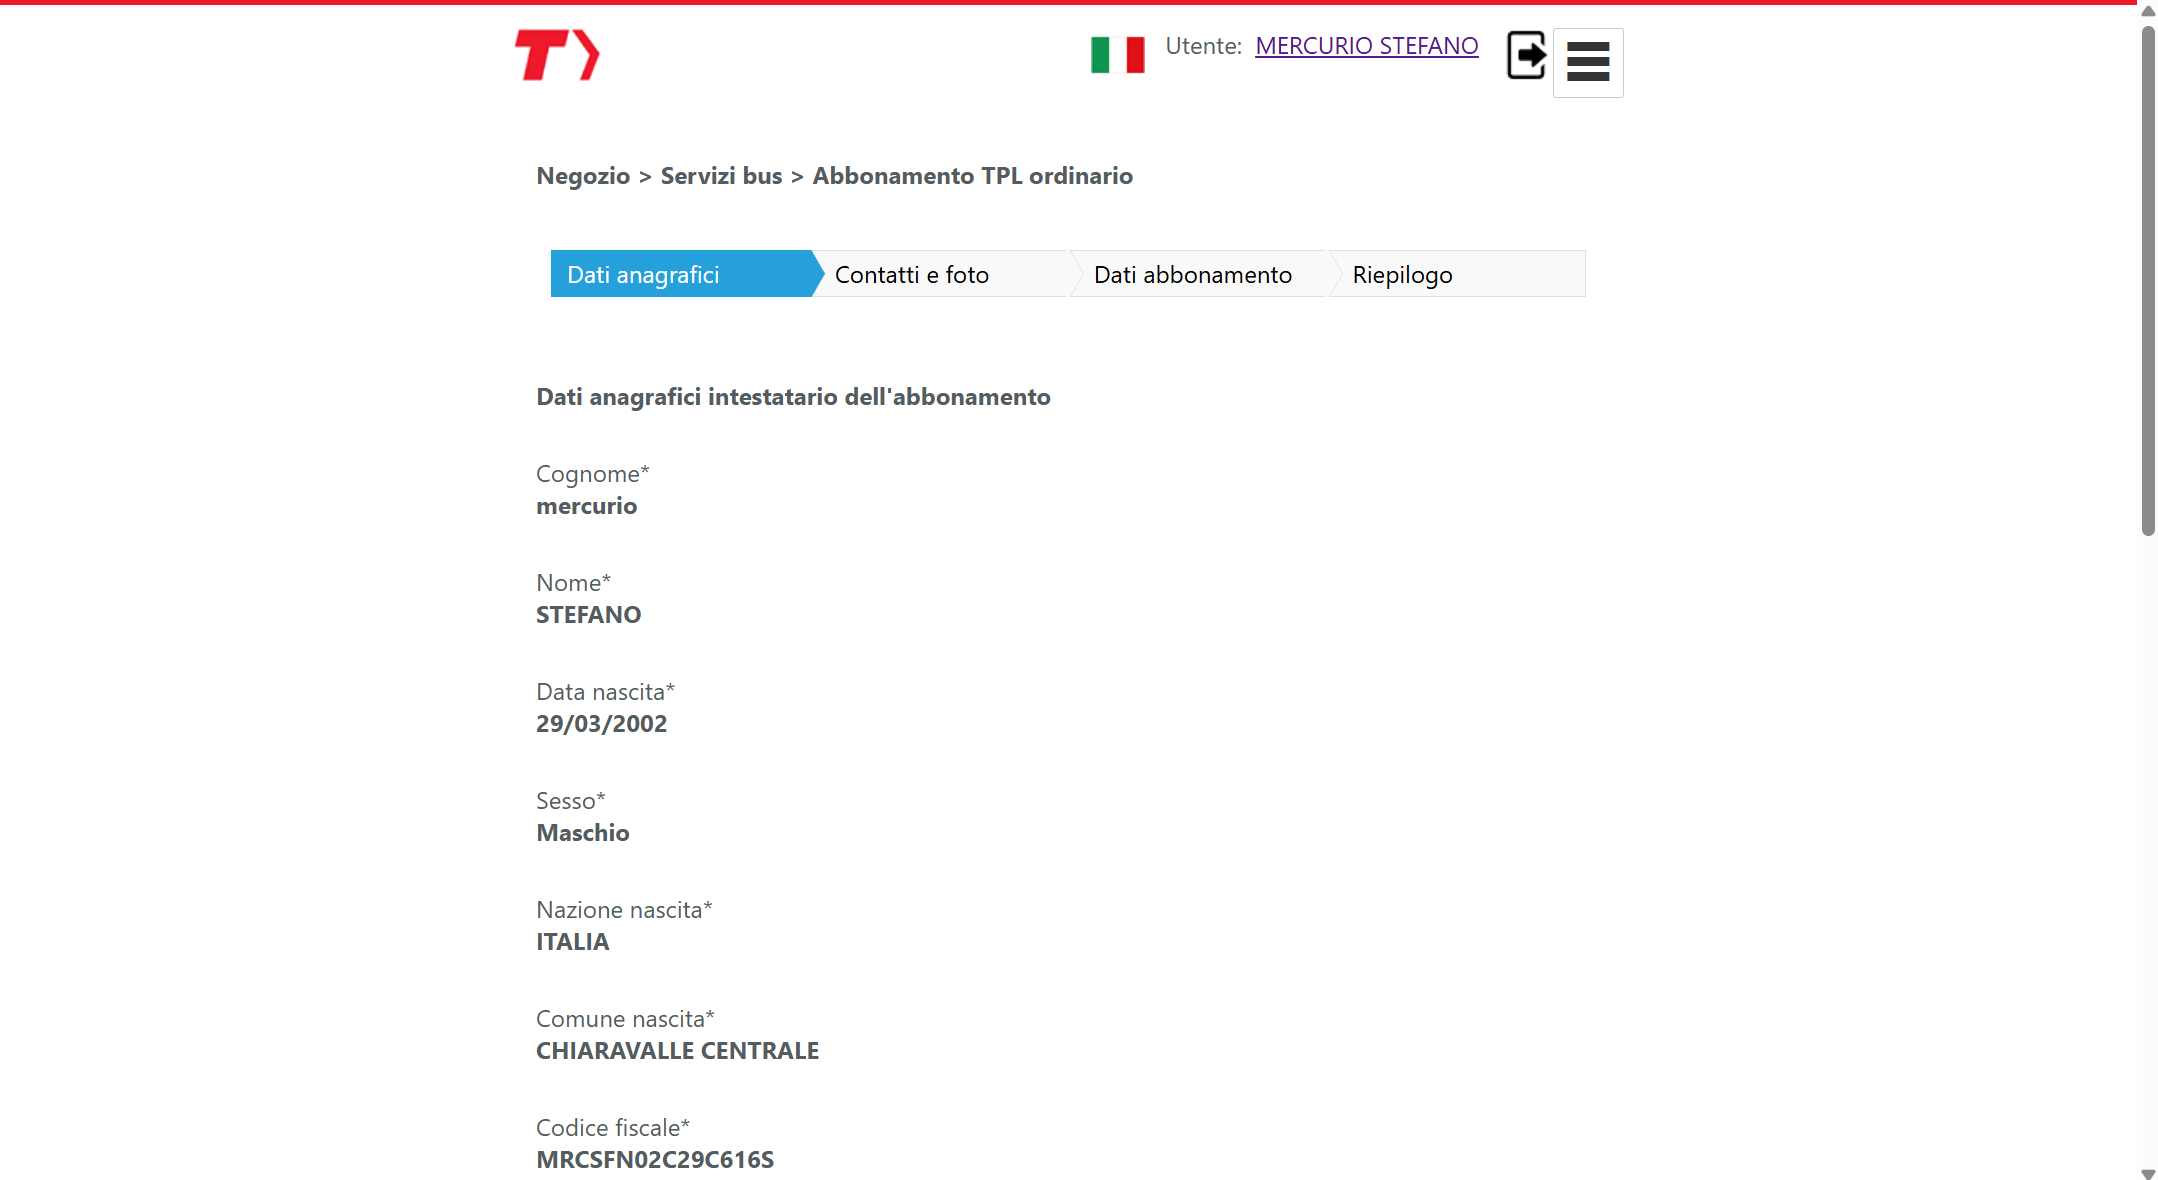
\includegraphics[width=\textwidth]{Tper sito originale/FlussoAcquistoS.png}
\par\small\textit{Before: flusso acquisto originale --- registrazione obbligatoria, nessuna guida}
\end{minipage}
\hfill
\begin{minipage}[t]{0.498\textwidth}
\centering
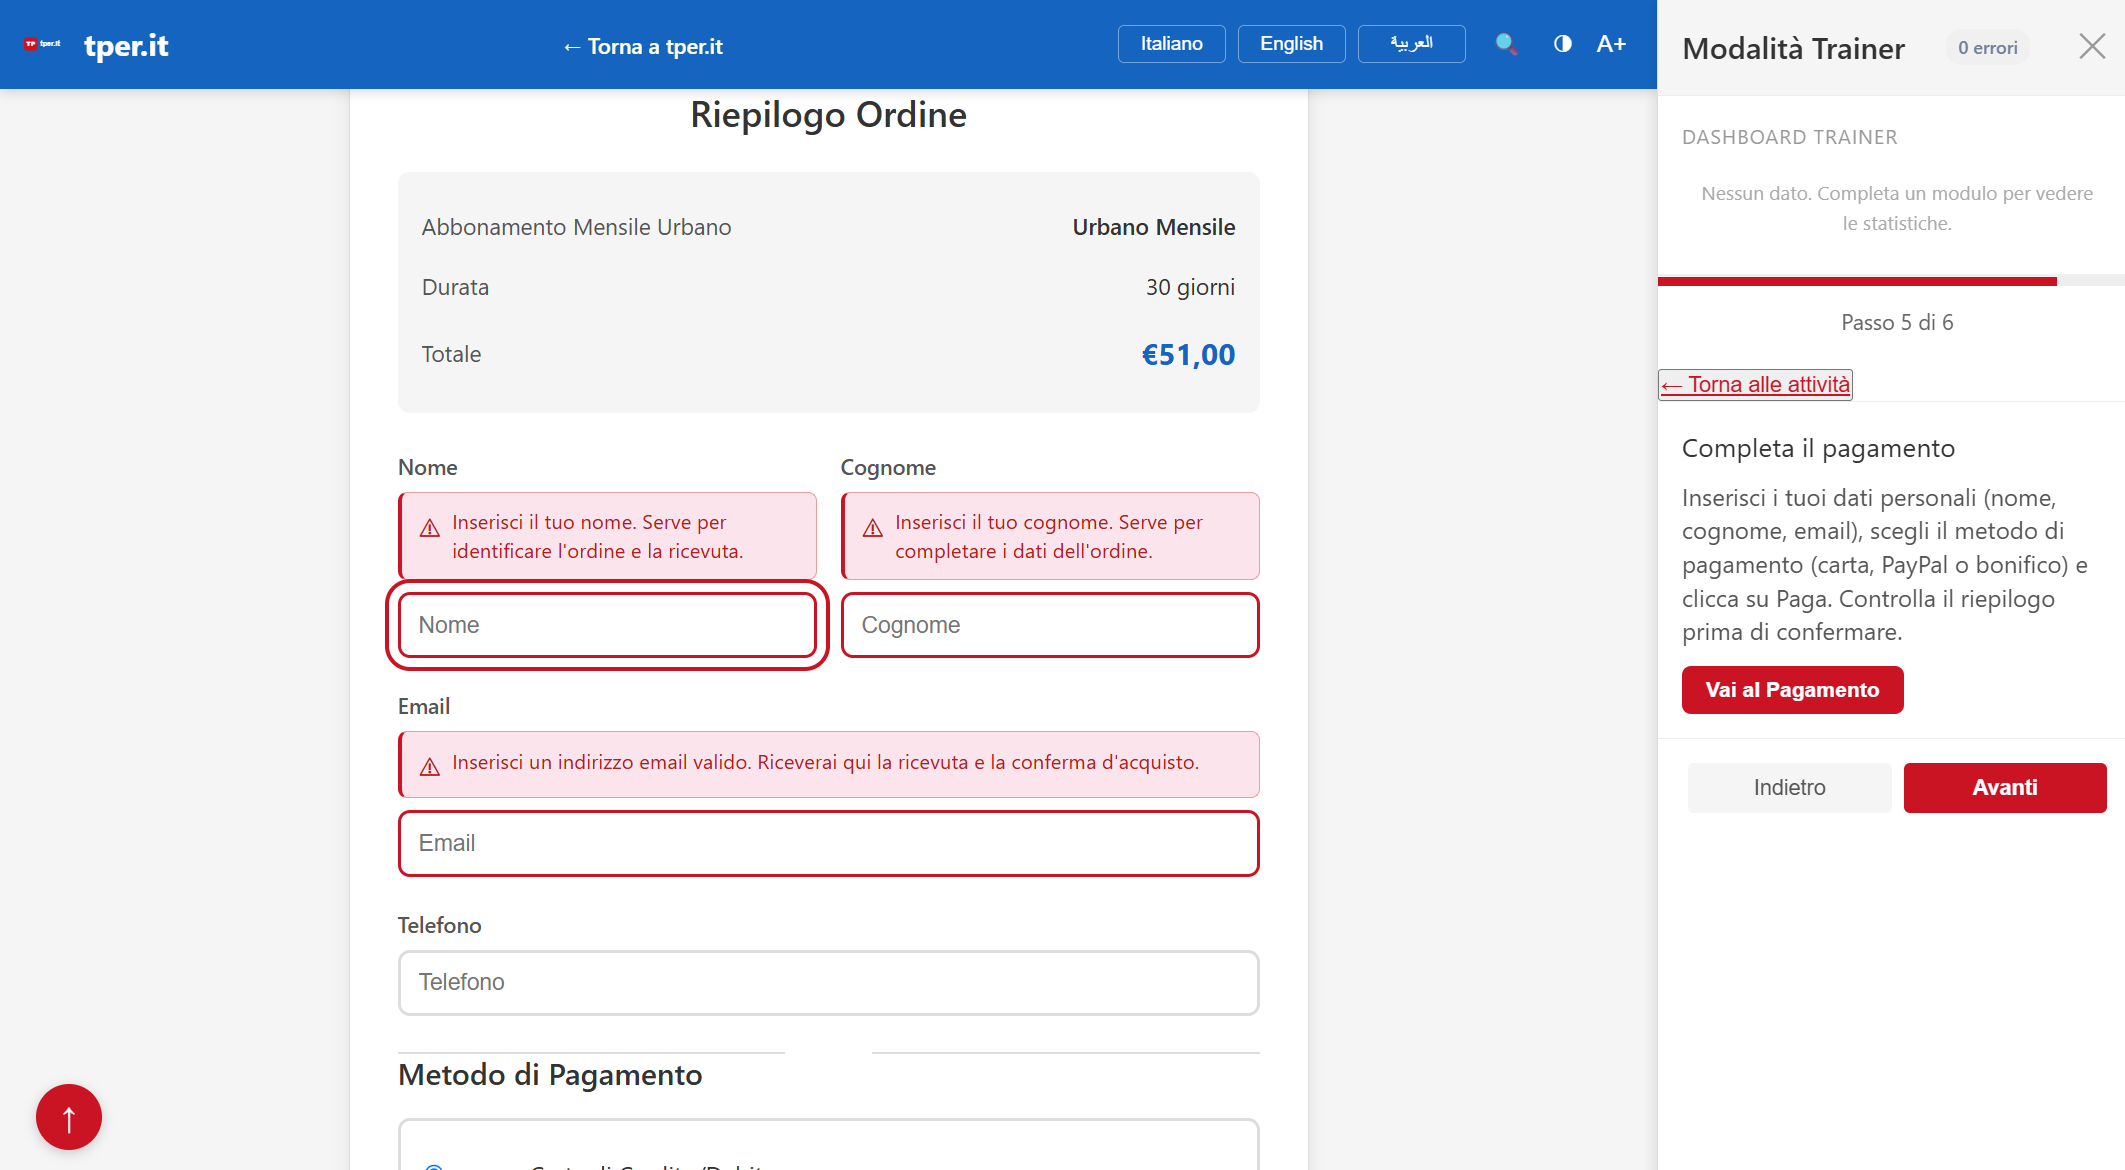
\includegraphics[width=\textwidth]{Redesign Tper 2.0/RiepilogoS.png}
\par\small\textit{After: flusso acquisto 2.0 --- barra progresso, form guidato, riepilogo}
\end{minipage}
\caption{Flusso Acquisto \texttt{solweb.tper.it}}
\label{fig:comparison-acquisto}
\end{figure}

\begin{table}[H]
\centering
\small
\renewcommand{\arraystretch}{1.4}
\begin{tabular}{|p{0.5cm}|p{7cm}|p{7cm}|}
\hline
& \textbf{Before} & \textbf{After} \\ \hline
\cellcolor{primaryColor!15} &
\textit{Flusso acquisto solweb originale} &
\textit{Flusso acquisto solweb 2.0} \\ \hline

\raisebox{0.5cm}{\rotatebox{90}{\textbf{Progresso}}} &
Nessun indicatore di progresso. L'utente non sa a che punto è del processo né quanti passi mancano. Abbandono frequente per disorientamento (Issue D2). &
\textbf{Barra di progresso a 4 passi}: Accedi $\rightarrow$ Scegli il Piano $\rightarrow$ Documenti $\rightarrow$ Pagamento. Ogni passo mostra: numero del passo, descrizione testuale, indicatore grafico di completamento (verde = completato, rosso = attivo). Visibile su tutte le pagine del flusso (R3). \\ \hline

\raisebox{0.5cm}{\rotatebox{90}{\textbf{Documenti}}} &
Nessuna checklist preventiva. L'utente scopre quali documenti servono solo dopo aver iniziato il flusso, spesso causando abbandono a metà. Utenti anziani costretti a tornare allo sportello perché privi dei documenti (R11). &
\textbf{Checklist interattiva} con barra di progresso (0/4 $\rightarrow$ 4/4). 4 card documento con riproduzione visiva del documento reale (dov'è il numero, dov'è la scadenza). Checkbox ``Ho questo documento''. Caricamento guidato. Badge ``Documenti necessari'' visibile prima di iniziare (R11). \\ \hline

\raisebox{0.5cm}{\rotatebox{90}{\textbf{Pagamento}}} &
Form di pagamento senza riepilogo ordine. Nessuna icona di sicurezza. Messaggi di errore generici: ``Errore --- riprovare''. L'utente non sa cosa ha sbagliato né come correggere (Issue D4). &
\textbf{Riepilogo ordine} sempre visibile: piano, durata, totale. 3 metodi di pagamento con radio button (Carta, PayPal, Bonifico). Checkbox termini. Messaggi di errore esponenziali: cosa è successo + perché + come risolvere + alternativa (R10). \\ \hline

\raisebox{0.5cm}{\rotatebox{90}{\textbf{Flessibilità}}} &
Unico percorso possibile: registrazione $\rightarrow$ login $\rightarrow$ acquisto. Nessuna variante per ricarica, rinnovo impersonale o sanzioni (Issue D5). &
\textbf{Multi-flusso}: pagamento.html gestisce 4 flussi diversi (acquisto, rinnovo, ricarica, sanzioni) con breadcrumb e form adattivi. Il percorso guest per rinnovo impersonale e ricarica salta completamente la registrazione (R7). \\ \hline
\end{tabular}
\caption{Flusso Acquisto solweb}
\label{tab:comparison-acquisto}
\end{table}

\vspace{0.3cm}

% ============================================================
% CONFRONTO 5: RIEPILOGO POST-ACQUISTO
% ============================================================
\section{Riepilogo Post-Acquisto \texttt{solweb.tper.it}}
\label{sec:comparison-riepilogo}

\textbf{UR-02 $\rightarrow$ R6} --- PDF scambiato per biglietto valido $\rightarrow$ 3 passi guidati post-acquisto. Rischio multa a bordo.

\begin{figure}[H]
\centering
\begin{minipage}[t]{0.498\textwidth}
\centering
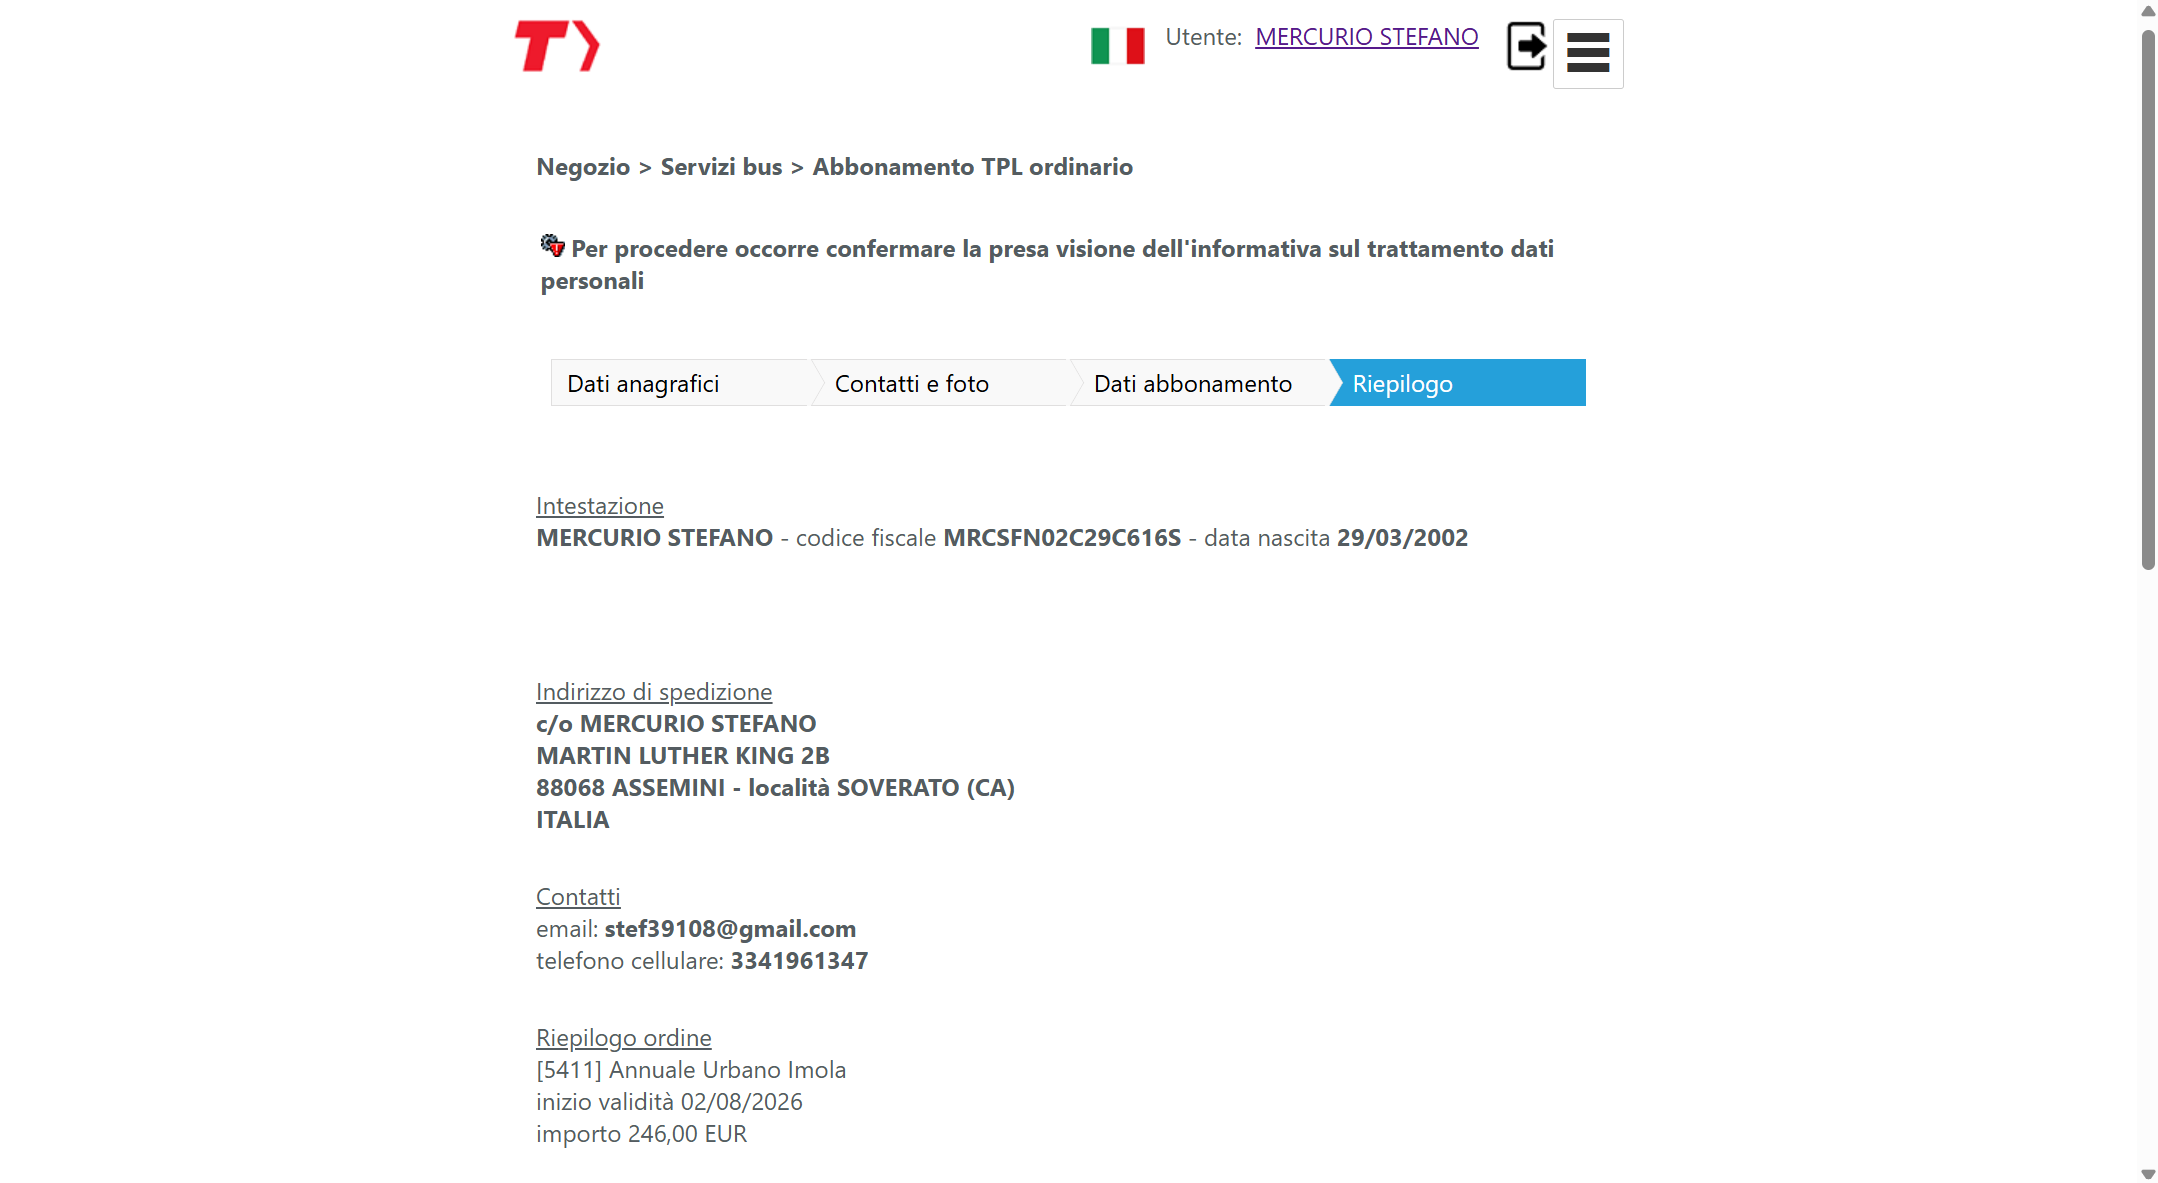
\includegraphics[width=\textwidth]{Tper sito originale/RiepilogoS.png}
\par\small\textit{Before: riepilogo originale --- solo conferma, nessuna guida post-acquisto}
\end{minipage}
\hfill
\begin{minipage}[t]{0.498\textwidth}
\centering
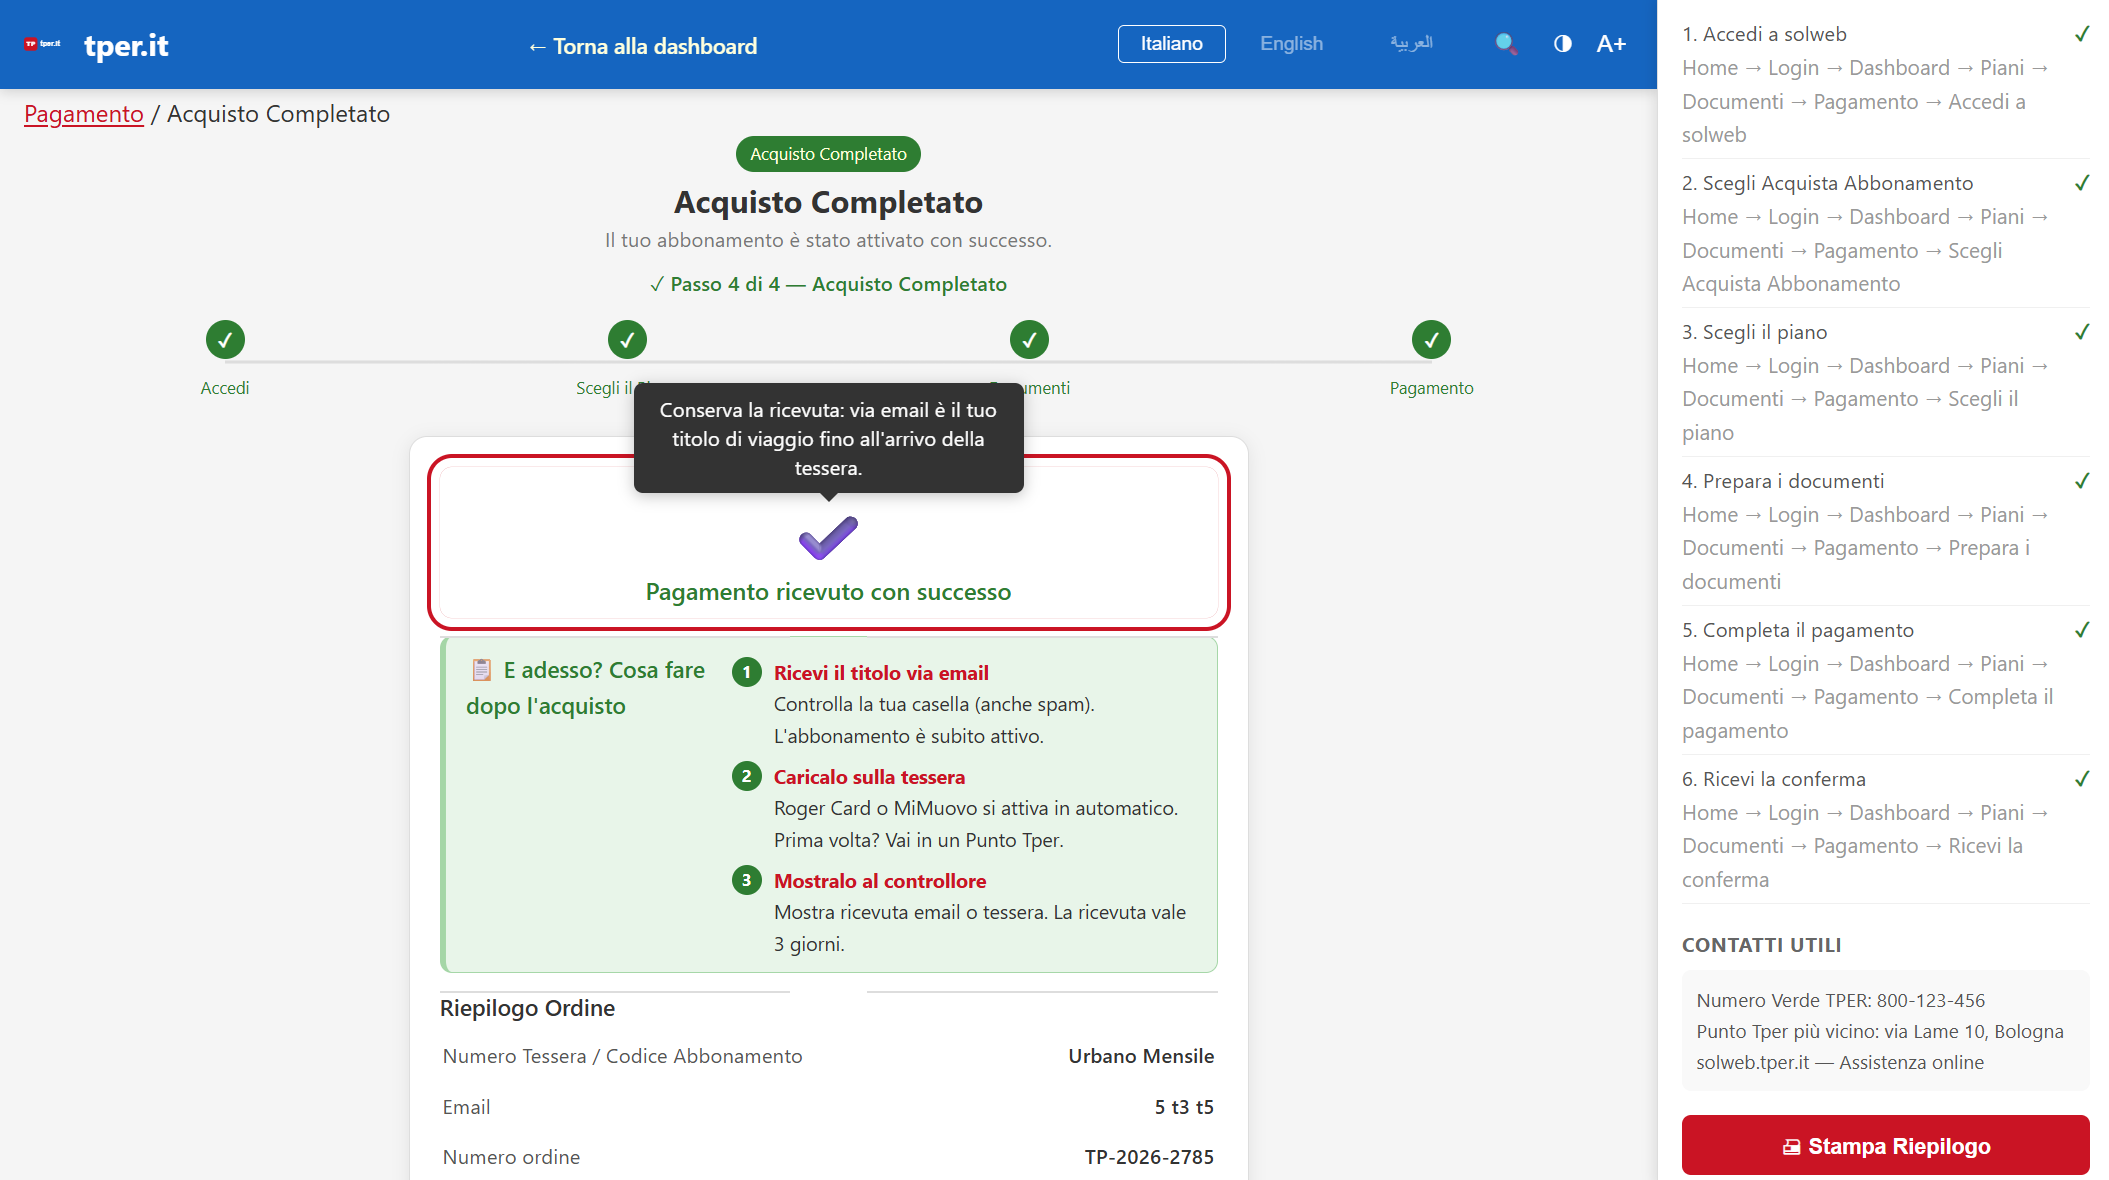
\includegraphics[width=\textwidth]{Redesign Tper 2.0/AcquistoS.png}
\par\small\textit{After: conferma 2.0 --- 3 passi guidati + ricevuta stampabile}
\end{minipage}
\caption{Riepilogo Post-Acquisto}
\label{fig:comparison-riepilogo}
\end{figure}

\begin{table}[H]
\centering
\small
\renewcommand{\arraystretch}{1.4}
\begin{tabular}{|p{0.5cm}|p{7cm}|p{7cm}|}
\hline
& \textbf{Before} & \textbf{After} \\ \hline
\cellcolor{primaryColor!15} &
\textit{Riepilogo originale post-acquisto} &
\textit{Conferma post-acquisto in solweb 2.0} \\ \hline

\raisebox{0.5cm}{\rotatebox{90}{\textbf{Conferma}}} &
Messaggio scarno di conferma. Nessuna spiegazione di cosa accade dopo. Il PDF generato viene scambiato per un titolo di viaggio valido --- ma non lo è (UR-02). &
\textbf{H1}: ``Grazie per il tuo acquisto!''. Barra di progresso completa (4/4 con spunta verde). Riepilogo ordine dettagliato: piano, email, numero ordine, metodo di pagamento, totale. Pulsante ``Scarica Ricevuta (PDF)'' (R6). \\ \hline

\raisebox{0.5cm}{\rotatebox{90}{\textbf{Istruzioni}}} &
\textbf{Assenti.} Nessuna guida su come utilizzare il biglietto/abbonamento acquistato. L'utente non sa se deve stampare qualcosa, mostrare il telefono, o validare una tessera (UR-02). &
\textbf{3 passi guidati post-acquisto}: (1) Riceverai una email di conferma con i dettagli dell'ordine, (2) La tua tessera si attiverà automaticamente entro 24 ore, (3) Mostra la tessera al controllore a bordo. Ogni passo è numerato e illustrato con icone (R6, UR-02). \\ \hline

\raisebox{0.5cm}{\rotatebox{90}{\textbf{Supporto}}} &
Nessun link di supporto post-acquisto. L'utente in difficoltà deve cercare autonomamente il servizio clienti. &
Link all'aiuto sempre visibile. Riferimento al numero ordine per assistenza. Possibilità di tornare alla dashboard o alla home. \\ \hline

\raisebox{0.5cm}{\rotatebox{90}{\textbf{Multicanale}}} &
Nessuna connessione con altri canali. Il percorso termina senza indicazioni su come usare il servizio acquistato su Roger, al Punto Tper o a bordo. &
Riferimenti cross-canale: se hai acquistato un abbonamento, ti spieghiamo come usarlo anche sull'App Roger. Se hai pagato una sanzione, ti indichiamo come verificare lo stato (UR-02, R6). \\ \hline
\end{tabular}
\caption{Riepilogo Post-Acquisto}
\label{tab:comparison-riepilogo}
\end{table}

\vspace{0.3cm}

% ============================================================
% CONFRONTO 6: TRAINER MODE E SUPPORTO
% ============================================================
\section{Trainer Mode e Supporto}
\label{sec:comparison-trainer}

\textbf{R5 $\rightarrow$ R4+R5+R6} --- Nessun trainer $\rightarrow$ Sidebar 22 pagine, 5 moduli, script operatore. Maria 0/5 task, SUS 27.5.

\begin{figure}[H]
\centering
\begin{minipage}{0.498\textwidth}
\centering
\rule{\textwidth}{0.1pt}
\vspace{2cm}
\rule{\textwidth}{0.1pt}
\par\small\textit{Before: nessun trainer mode --- solo help desk telefonico}
\end{minipage}
\hfill
\begin{minipage}[t]{0.498\textwidth}
\centering
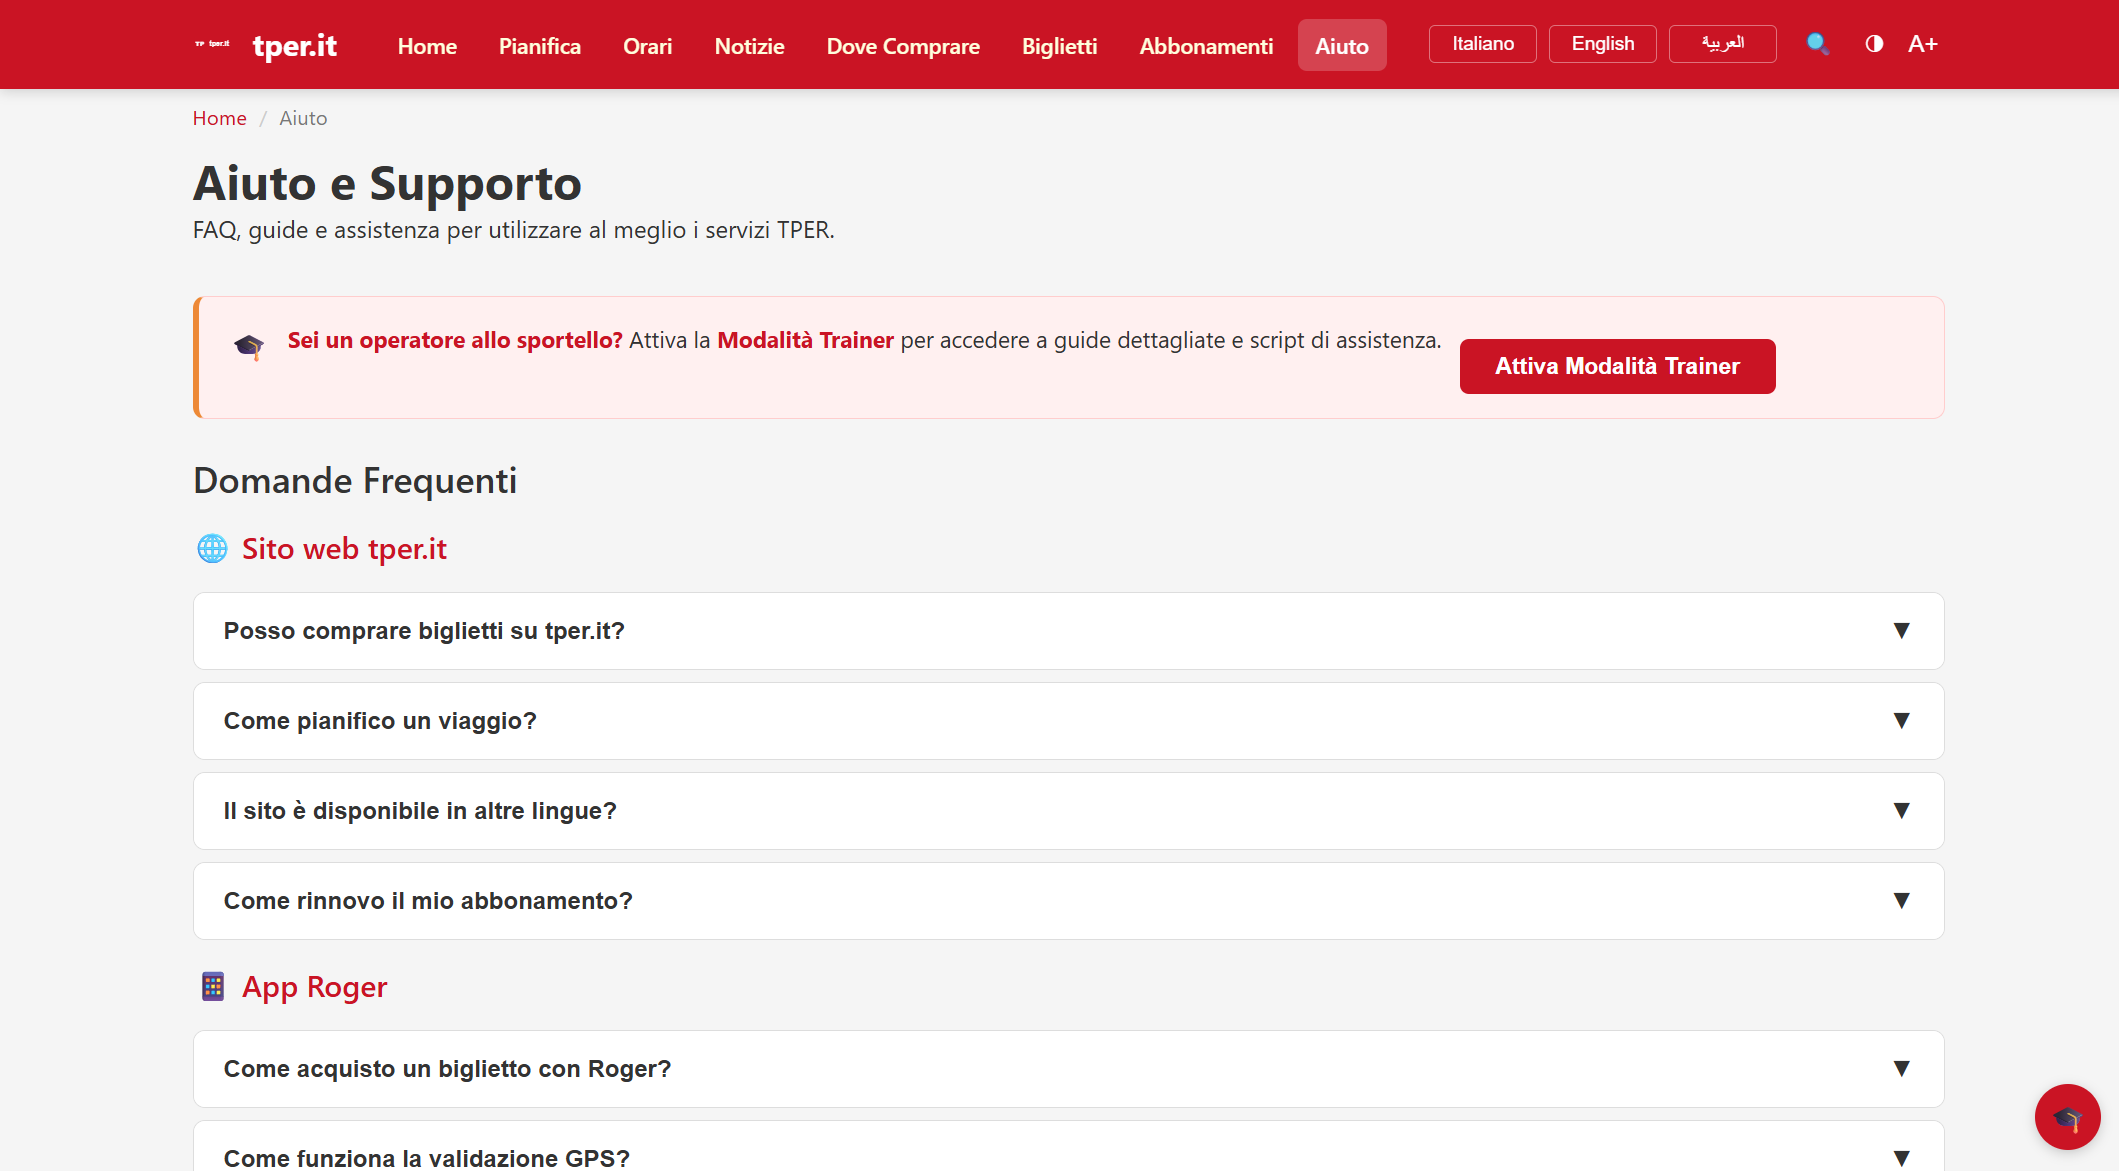
\includegraphics[width=\textwidth]{Redesign Tper 2.0/Aiuto.png}
\par\small\textit{After: sezione Aiuto con trainer mode, FAQ, guide passo-passo}
\end{minipage}
\caption{Trainer Mode e Supporto}
\label{fig:comparison-trainer}
\end{figure}

\begin{table}[H]
\centering
\small
\renewcommand{\arraystretch}{1.4}
\begin{tabular}{|p{0.5cm}|p{7cm}|p{7cm}|}
\hline
& \textbf{Before} & \textbf{After} \\ \hline
\cellcolor{primaryColor!15} &
\textit{Supporto attuale su \texttt{tper.it}} &
\textit{Trainer-mode e supporto in tper 2.0} \\ \hline

\raisebox{0.5cm}{\rotatebox{90}{\textbf{Trainer}}} &
\textbf{Inesistente.} Nessuna modalità assistita per operatori allo sportello. Nessun meccanismo di guida passo-passo per accompagnare utenti a bassa competenza digitale nell'orientamento tra i canali. L'unico canale di supporto è il servizio clienti (telefonico o email) (R4, R5). &
\textbf{Barra laterale integrata} su tutte le 22 pagine del sito. 5 moduli trainer: Rinnovo, Acquista, Viaggio, Biglietto, Ricarica. Ogni modulo carica automaticamente la pagina corretta con gli highlight sugli elementi rilevanti. Attivazione: su richiesta (pulsante $\mathcal{T}$) o automatica dopo 2 errori consecutivi dell'utente (R4, R5). \\ \hline

\raisebox{0.5cm}{\rotatebox{90}{\textbf{Script}}} &
Nessuno script operativo per il personale di sportello. &
Script a 5 passi per operatori: (1) Identifica il bisogno, (2) Consiglia il titolo di viaggio, (3) Indirizza al canale corretto, (4) Spiega la validazione, (5) Conferma e chiedi se serve altro (R4). \\ \hline

\raisebox{0.5cm}{\rotatebox{90}{\textbf{FAQ}}} &
Solo help desk come canale di supporto. Nessuna guida interattiva, nessun FAQ organizzato (R10). &
\textbf{Accordion FAQ raggruppato per canale}: \texttt{tper.it}, App Roger, Punti Tper e Rivendite, Sanzioni, Contactless a Bordo. Ogni sezione risponde alle domande più comuni per quel canale. Include link diretti (es. da FAQ solweb $\rightarrow$ pagina di acquisto) (R9, R10). \\ \hline

\raisebox{0.5cm}{\rotatebox{90}{\textbf{Guide}}} &
Assenti. &
3 card guida passo-passo nella sezione Aiuto: ``Come acquistare su solweb'', ``Come usare Roger App'', ``Come trovare un Punto Tper''. Ciascuna con CTA diretta al canale corrispondente. Wizard interattivi su Dove Comprare, Biglietti e Abbonamenti (R9). \\ \hline

\raisebox{0.5cm}{\rotatebox{90}{\textbf{Persistenza}}} &
Nessuna memoria di sessione. Se l'utente chiude il browser o scade il timeout, perde tutto e deve ricominciare da capo. &
\textbf{Auto-salvataggio} dello stato della sessione trainer in localStorage. L'utente può riprendere dal punto esatto in cui si era interrotto. Riepilogo stampabile con screenshot annotati e percorso di navigazione (R5, R6). \\ \hline
\end{tabular}
\caption{Trainer Mode e Supporto}
\label{tab:comparison-trainer}
\end{table}

\vspace{0.3cm}

% ============================================================
% CONFRONTO 7: ACCESSIBILITÀ E MULTILINGUA
% ============================================================
\section{Accessibilità e Multilingua}
\label{sec:comparison-a11y}

\textbf{R3+D3 $\rightarrow$ R8+R12} --- Solo IT, 10pt, target <44px $\rightarrow$ IT/EN/AR, 14pt, WCAG AA. Chris 3/5 falliti per lingua.

\begin{table}[H]
\centering
\small
\renewcommand{\arraystretch}{1.4}
\begin{tabular}{|p{0.5cm}|p{7cm}|p{7cm}|}
\hline
& \textbf{Before} & \textbf{After} \\ \hline
\cellcolor{primaryColor!15} &
\textit{Stato attuale del sito \texttt{tper.it} live} &
\textit{Accessibilità e lingue in tper 2.0} \\ \hline

\raisebox{0.5cm}{\rotatebox{90}{\textbf{Lingua}}} &
\textbf{Solo italiano.} Nessun selettore di lingua, nessun contenuto in inglese o arabo. Utenti stranieri completamente esclusi dai servizi informativi online. Chris H. (inglese): 3/5 task falliti nonostante alta competenza digitale (R12). &
\textbf{IT + EN + AR.} Commutatore lingua a tre pulsanti sempre visibile nell'header di ogni pagina. Traduzione completa delle label, dei contenuti informativi, delle FAQ e dei wizard. 1.600+ chiavi i18n nei file JavaScript. Supporto RTL per l'arabo (R12). \\ \hline

\raisebox{0.5cm}{\rotatebox{90}{\textbf{Carattere}}} &
Testo piccolo (10--11pt). Difficoltà di lettura per utenti over 65, particolarmente critico per i nomi dei canali e le tariffe. Maria B. non distingueva pulsanti da testo statico (R8). &
\textbf{Minimo 14pt} su tutti i testi. Pulsante \textbf{A+} nell'header per ingrandire ulteriormente il carattere con un click. Toggle persistente tra le pagine (R8). \\ \hline

\raisebox{0.5cm}{\rotatebox{90}{\textbf{Contrasto}}} &
Contrasto non dichiarato, verosimilmente inferiore allo standard WCAG AA per alcune combinazioni colore. &
\textbf{Rapporto minimo 4.5:1} (WCAG AA). Pulsante \textbf{$\blacksquare$} per attivare/disattivare la modalità contrasto elevato su tutte le pagine. Toggle persistente. Palette completamente rivista in modalità alto contrasto (R8). \\ \hline

\raisebox{0.5cm}{\rotatebox{90}{\textbf{ARIA}}} &
Skip link ``Salta al contenuto principale'' presente. Ruoli ARIA assenti o parziali sulla maggior parte degli elementi interattivi. &
\textbf{ARIA completo}: \texttt{role="banner"}, \texttt{role="navigation"}, \texttt{role="main"}, \texttt{role="complementary"} (trainer bar), \texttt{role="contentinfo"} (footer), \texttt{role="dialog"} (modali e search overlay), \texttt{role="search"} (route planner), \texttt{aria-label} su tutti gli elementi interattivi, \texttt{aria-current="page"} sulla pagina attiva, \texttt{aria-expanded} su hamburger e accordion, \texttt{aria-modal="true"} su overlay e modali (R8). \\ \hline

\raisebox{0.5cm}{\rotatebox{90}{\textbf{Target}}} &
Touch target inferiori a 44$\times$44px in molte aree, rendendo difficile l'uso su smartphone per utenti con ridotta destrezza. &
\textbf{Tutti i target interattivi $\ge$ 44$\times$44px} (WCAG 2.1). Pulsanti, link, checkbox e radio button dimensionati per interazione tattile senza errori (R8). \\ \hline
\end{tabular}
\caption{Accessibilità e Multilingua}
\label{tab:comparison-a11y}
\end{table}

\vspace{0.3cm}

% ============================================================
% CONFRONTO 8: TONO E TERMINOLOGIA
% ============================================================
\section{Tono e Terminologia}
\label{sec:comparison-tone}

\textbf{D3 $\rightarrow$ R9} --- Terminologia aziendale $\rightarrow$ Linguaggio utente + glosse. ``MiMuovo'', ``Rete di vendita'' incomprensibili a tutti i soggetti.

\begin{table}[H]
\centering
\small
\renewcommand{\arraystretch}{1.4}
\begin{tabular}{|p{0.5cm}|p{7cm}|p{7cm}|}
\hline
& \textbf{Before} & \textbf{After} \\ \hline
\cellcolor{primaryColor!15} &
\textit{Linguaggio attuale su \texttt{tper.it}} &
\textit{Tono e terminologia in tper 2.0} \\ \hline

\raisebox{0.5cm}{\rotatebox{90}{\textbf{Tono}}} &
Burocratico e istituzionale. Frasi impersonali, lessico da pubblica amministrazione. Messaggi di errore freddi e generici. L'utente si sente un ``praticante'' piuttosto che un cliente (Issue D3). &
Incoraggiante e inclusivo. Linguaggio in prima persona plurale: ``Ti aiutiamo a scegliere'', ``Nessun problema, possiamo riprovare insieme''. Messaggi di errore con tono umano e via d'uscita: ``Non hai trovato quello che cercavi? Prova con una di queste alternative'' (R9). \\ \hline

\raisebox{0.5cm}{\rotatebox{90}{\textbf{Termini}}} &
Terminologia esclusivamente aziendale: \textit{Rete di vendita}, \textit{Emettitrici automatiche}, \textit{MiMuovo}, \textit{SaltaSu}, \textit{Prontobus}, \textit{Discobus}. \texttt{solweb} e \textit{Roger} mai spiegati né introdotti. L'utente deve conoscere il gergo TPER prima di usare il sito (Issue D3). &
\textbf{Terminologia utente-centrica con glosse}: ``Dove Comprare'' (non ``Rete di vendita''), ``Abbonamenti online (solweb)'', ``Biglietti digitali (Roger)'', ``Tabaccherie e PuntoLis''. Ogni termine tecnico è accompagnato da una spiegazione inline o da un tooltip al primo utilizzo. Il nome aziendale resta tra parentesi per riferimento (R2, R9). \\ \hline

\raisebox{0.5cm}{\rotatebox{90}{\textbf{Messaggi}}} &
Messaggi di sistema impersonali e privi di guida. ``Errore --- riprovare'' senza spiegazione di causa o soluzione. L'utente abbandona il flusso (Issue D4). &
\textbf{Messaggi esponenziali} (R10): cosa è successo, perché è successo, come risolvere, cosa fare in alternativa. Box con sfondo a contrasto e icona di avviso, posizionato inline sopra il campo interessato. Micro-rinforzi dopo ogni passo: ``Perfetto, questo è fatto!'' (R9). \\ \hline

\raisebox{0.5cm}{\rotatebox{90}{\textbf{Onboarding}}} &
Nessun percorso di primo accesso. L'utente arriva sulla homepage e deve capire tutto da solo. Maria B.: \textit{``non so neanche da dove cominciare''}. &
\textbf{Tour ``Prima Volta''}: 4 schermate illustrate che spiegano i canali tramite metafore quotidiane. Attivabile dal pulsante Aiuto. Linguaggio rassicurante: ``Non preoccuparti, ti spiego dove andare'' (R9). \\ \hline
\end{tabular}
\caption{Tono e Terminologia}
\label{tab:comparison-tone}
\end{table}

\vspace{0.5cm}

% ============================================================
% RIEPILOGO
% ============================================================
\section{Riepilogo delle Differenze Chiave}
\label{sec:comparison-summary}

\begin{tcolorbox}[colback=backgroundColor,colframe=primaryColor,arc=2mm]
{\small
\renewcommand{\arraystretch}{1.3}
\begin{tabular}{|p{3.5cm}|p{5cm}|p{5cm}|}
\hline
\textbf{Dimensione} & \textbf{Before (\texttt{tper.it} live)} & \textbf{After (tper 2.0)} \\ \hline
Homepage \texttt{tper.it} & News aziendali e slider istituzionale (D1) & Hero pianificatore + griglia 6 card task-oriented (R1) \\ \hline
Homepage \texttt{solweb} & Solo login, nessun percorso guest (D5) & 4 azioni rapide senza registrazione + progress bar (R7) \\ \hline
Architettura Informativa & 3 pagine sovrapposte (Biglietti, Abbonamenti, Tariffe), canali sepolti al 3\textdegree{} livello (D2) & 3 pagine specializzate: Biglietti, Abbonamenti, Dove Comprare --- ogni pagina, un compito (R2) \\ \hline
Navigazione & Mega-menu 200+ voci, 5 livelli di profondità & Nav flat 8 voci + breadcrumb su tutte le pagine \\ \hline
``Dove Comprare'' & Inesistente --- \textit{Rete di vendita} sepolta & Sezione autonoma + wizard 3 domande + tabella comparativa 5$\times$7 \\ \hline
solweb / Roger & Mai menzionati in homepage & Card dedicate con CTA dirette e modale di transizione \\ \hline
Guida canali & Assente --- scelta affidata all'utente & Wizard interattivi su 3 pagine + tabella comparativa \\ \hline
Flusso acquisto & Senza progresso, senza checklist documenti & Barra 4 passi + checklist interattiva (R3, R11) \\ \hline
Post-acquisto & Nessuna istruzione, PDF scambiato per biglietto (UR-02) & 3 passi guidati + ricevuta stampabile (R6) \\ \hline
Trainer Mode & Inesistente (R5) & Barra laterale su 22 pagine + 5 moduli + persistenza + riepilogo (R4, R5, R6) \\ \hline
FAQ / Guide & Solo help desk & Accordion per canale + 3 guide passo-passo + script operatore \\ \hline
Lingua & Solo italiano & IT + EN + AR, 1.600+ chiavi i18n, supporto RTL (R12) \\ \hline
Carattere / Contrasto & 10--11pt, sotto WCAG AA & 14pt min, 4.5:1, toggle A+, toggle contrasto (R8) \\ \hline
ARIA / Touch target & Parziale, target $<$ 44px & Completo: ruoli, label, stati; tutti i target $\ge$ 44$\times$44px (R8) \\ \hline
Tono & Burocratico/istituzionale & Incoraggiante/inclusivo + micro-rinforzi (R9) \\ \hline
Terminologia & Aziendale (Rete di vendita, MiMuovo, Emettitrici) & Utente-centrica con glosse (Dove Comprare, Abbonamenti online) \\ \hline
Errori & Messaggi generici ``Errore --- riprovare'' & Messaggi esponenziali: causa + soluzione + alternativa (R10) \\ \hline
Messaggio informativo & Assente & Banner ``tper.it è un sito informativo'' su ogni pagina (R1) \\ \hline
Documenti & Nessuna checklist preventiva & Checklist interattiva con riproduzione visiva (R11) \\ \hline
Guest path & Inesistente --- login obbligatorio per tutto & Rinnovo impers., ricarica, sanzioni senza registrazione (R7) \\ \hline
\end{tabular}
}
\end{tcolorbox}

\vspace{0.5cm}

\begin{center}
{\color{secondaryColor}\small
Documento compilato sulla base dell'analisi diretta dei siti \texttt{tper.it} e \texttt{solweb.tper.it} live, \\
delle raccomandazioni R1--R13 della Phase B, e dei risultati dei test utente Phase A (4 soggetti, SUS 37.5/100) \\[4pt]
\textbf{Phase C --- Design Proposal: Before/After Comparison} \\[4pt]
Progetto: UX Design Project: Help People Help People --- TPER S.p.A.}
\end{center}


% ================================================================
% Design Card: Final Reflections
% ================================================================

\newpage

\section{Design Card --- Final Reflections}
\label{sec:design-card}

\input{Comparison/00-reflections-body.tex}

% ================================================================
% Design Summary Card
% ================================================================

\newpage

\section{Design Summary Card}
\label{sec:design-summary}

\begin{tcolorbox}[colback=primaryColor,colframe=primaryColor,arc=1.5mm,halign=center,valign=center,height=2cm]
 \color{white}\LARGE\bfseries\sffamily DESIGN SUMMARY \\[0.1cm]
 \color{white!80}\small\sffamily Phase C --- Design Proposal
\end{tcolorbox}

\vspace{0.3cm}

\subsection*{Design Versions as Submitted}

\begin{table}[H]
\centering
\small
\renewcommand{\arraystretch}{1.3}
\begin{tabular}{|p{2.5cm}|p{3.5cm}|p{3.5cm}|p{3.5cm}|}
\hline
\textbf{Versione} & \textbf{Cartella} & \textbf{Data / Ora} & \textbf{Tipi di valutazione} \\
\hline
\textbf{V0} 
& \texttt{Website - Finale/} (stato iniziale)
& 28 Giugno 2026, ore 18:00
& Ante valutazione formale \\
\hline
\textbf{V1} 
& \texttt{Website - Finale/} (post-FT fix)
& 2 Luglio 2026, ore 12:00
& Valutazione ispettiva --- Cognitive Walkthrough (CW-01--CW-09) \\
\hline
\textbf{Finale (v2.0)} 
& \texttt{Website - Finale/} (versione finale)
& 4 Luglio 2026, ore 10:00
& \begin{tabular}{@{}l@{}}
--- Cognitive Walkthrough (Post-Fix) \\ 
--- Formative Test (2 soggetti) \\
--- Summative Test (2 soggetti)
\end{tabular} \\
\hline
\end{tabular}
\caption{Versioni di design sottoposte a valutazione}
\label{tab:design-versions}
\end{table}

\vspace{0.3cm}

\subsection*{List of Issues Handled During Redesign, Ordered by Importance}

\renewcommand{\arraystretch}{1.3}
\begin{longtable}{|p{0.8cm}|p{3cm}|p{3.5cm}|p{6.5cm}|}
\hline
\textbf{\#} & \textbf{Issue} & \textbf{Rif. Requirement / Test} & \textbf{Wireframe / Blueprint interessato} \\
\hline
\endhead
1 & Ambiguit\`a terminologica ``Dove Comprare'' vs ``Abbonamenti'' (\textbf{FT1}, P=5, I=5) 
& Phase A: R1 (Home Page Orientata al Compito) \\
& Phase B: Cast Card --- UR-03 \\
& Phase D: CW-04, CW-05
& WF1 (Homepage --- griglia ``Cosa vuoi fare?'' e sidebar canali) \\
& BP1 (Architettura Informazione: sezioni acquisto vs informativo) \\
& BP3 (User Journey: punto decisionale ``dove acquisto?'') \\
\hline
2 & Confusione tra canali di acquisto: utente non sa quale canale usare (\textbf{D2}, R4) 
& Phase A: R2 (IA Piana), R4 (Trainer-Mode) \\
& Phase B: Cast Card --- UR-01 \\
& Phase D: CW-02, FT2
& WF3 (Dove Comprare --- card canali con icone) \\
& BP2 (Ecosistema Multi-Canale: relazioni e bridge) \\
\hline
3 & Nessuna guida passo-passo per operazioni complesse (\textbf{R5}) 
& Phase A: R5 (Persistenza Progressi) \\
& Phase B: Cast Card --- UR-05 \\
& Phase D: CW-07
& WF5 (Aiuto + Trainer-Mode: guida 5 passi) \\
& BP3 (Intervento Trainer-Mode lungo il journey) \\
\hline
4 & Homepage sovraccarica: news aziendali oscurano funzioni primarie (\textbf{D1}, R1) 
& Phase A: R1 (Home Page Orientata al Compito) \\
& Phase D: CW-01
& WF1 (Homepage: hero search + 4 card servizi, news in footer) \\
& BP1 (IA: riorganizzazione sezioni per priorit\`a d'uso) \\
\hline
5 & Barriera terminologica: ``solweb'', ``Roger'' come nomi tecnici (\textbf{D3}, R2) 
& Phase A: R2 (Etichette Descrittive) \\
& Phase B: Cast Card --- Laura, Maria \\
& Phase D: FT1
& WF3 (Card canali: ``Abbonamenti online (solweb)'') \\
& BP2 (Ecosistema: etichettatura utente-centrica) \\
\hline
6 & Assenza di feedback e recupero dagli errori (\textbf{D4}, R10) 
& Phase A: R10 (Messaggi di Errore Esponenziali) \\
& Phase D: CW-08
& BP3 (Punti di decisione con messaggi di recupero) \\
& WF5 (Trainer-Mode: messaggi incoraggianti) \\
\hline
7 & Autenticazione obbligatoria per operazioni di base (\textbf{D5}, R7) 
& Phase A: R7 (Percorso Guest) \\
& Phase D: CW-06
& BP1 (IA: sezioni accessibili senza login) \\
& WF1 (Sidebar canali sempre visibile, anche in modalit\`a guest) \\
\hline
8 & Assenza supporto multilingua per utenti stranieri (\textbf{R12}) 
& Phase A: R12 (Inglese e Arabo) \\
& Phase B: Cast Card --- Fatima Hassan
& WF3 (Card canali e wizard tradotti in EN/AR) \\
& BP2 (Ecosistema: bridge con contenuti multilingua) \\
\hline
9 & Documentazione necessaria non anticipata all'utente (\textbf{R11}) 
& Phase A: R11 (Checklist Preventiva) \\
& Phase D: CW-09
& WF4 (Biglietti: badge ``Documenti necessari'') \\
& BP3 (Checklist prima del reindirizzamento a solweb) \\
\hline
10 & Assenza onboarding ``Primo Accesso'' (\textbf{FT2}, P=2, I=3) 
& Phase D: FT2, FT6
& WF5 (Tour guidato ``Prima Volta'' 4 schermate) \\
& BP3 (Punto di ingresso: onboarding prima navigazione) \\
\hline
\end{longtable}

\vspace{0.3cm}

\begin{tcolorbox}[colback=primaryColor!5,colframe=primaryColor,arc=2mm]
\small
\textbf{Nota:} Ogni issue \`e correlata ai requirement emersi dalla Phase A (R1--R13), dalla Phase B (Cast Card --- Use Case UR-01--UR-05) e dalla Phase D (Cognitive Walkthrough CW-01--CW-09, Formative Test FT1--FT7). Le soluzioni progettuali sono localizzabili nei wireframe (WF1--WF5) e nei blueprint (BP1--BP3).
\end{tcolorbox}

% ================================================================
% Fase D2: Inspection Card (Cognitive Walkthrough)
% ================================================================

\newpage

\section{Cognitive Walkthrough --- Inspection Card}
\label{sec:inspection-card}

\newcolumntype{L}[1]{>{\raggedright\arraybackslash}p{#1}}
\newcolumntype{C}[1]{>{\centering\arraybackslash}p{#1}}

\begin{tcolorbox}[colback=primaryColor,colframe=primaryColor,arc=3mm,halign=center,valign=center,height=2.5cm]
 \color{white}\LARGE\bfseries INSPECTION CARD \\[0.2cm]
 \color{white!80}\large UX Design Project: Help People Help People --- TPER S.p.A. \\[0.1cm]
 \color{white!60}\normalsize Phase D --- Cognitive Walkthrough
\end{tcolorbox}

\vspace{0.3cm}

% =====================================================================
% DATI DELL'INSPECTION (allineati al template)
% =====================================================================
\section{Dati dell'Inspection}

\begin{tcolorbox}[colback=backgroundColor,colframe=borderColor,arc=2mm]
\small

\noindent\textbf{Name of version:} Redesign TPER --- v1.0 (Phase C -- Design Proposal)

\vspace{0.3cm}
\noindent\textbf{Inspection context data:}
\begin{itemize}
 \item \textbf{Data:} 28-29 Giugno 2026
 \item \textbf{Team members:} 2 valutatori (membri del team di design)
 \item \textbf{Ruoli:} Valutatore 1 (narrator, guida la simulazione), Valutatore 2 (listener, annota le criticit\`a)
 \item \textbf{Modalit\`a:} Valutazione individuale su prototipo statico (HTML/CSS), seguita da confronto e consenso
\end{itemize}

\vspace{0.3cm}
\noindent\textbf{Inspection method:}
\begin{itemize}
 \item[$\bullet$] \textbf{Cognitive Walkthrough} (selezionato)
 \item[$\circ$] Formal Action Analysis
 \item[$\circ$] Informal Action Analysis
 \item[$\circ$] Heuristic Analysis
\end{itemize}

\vspace{0.3cm}
\noindent\textbf{Output of inspection:} Di seguito vengono documentati i 5 task analizzati. Per ogni passo vengono valutate le 4 domande del CW (Goal, Visibility, Mapping, Feedback). Per ogni criticit\`a rilevata viene fornita una giustificazione qualitativa.

\end{tcolorbox}

\vspace{0.3cm}

% =====================================================================
% INTRODUZIONE AL COGNITIVE WALKTHROUGH
% =====================================================================
\section{Introduzione al Cognitive Walkthrough}

\begin{tcolorbox}[colback=backgroundColor,colframe=borderColor,arc=2mm]
\small
Il Cognitive Walkthrough \`e un metodo ispettivo che valuta la facilit\`a di apprendimento tramite esecuzione simulata di task. Per ogni passo si risponde a 4 domande (Goal, Visibility, Mapping, Feedback). I valutatori simulano i profili delle personas definite in Phase B, assumendo competenza minima e contesto domestico senza assistenza.

\vspace{0.2cm}
\noindent\textbf{Task selezionati:}
\begin{enumerate}
 \item Rinnovo Abbonamento (Guest Flow)
 \item Acquisto Abbonamento (Login Flow)
 \item Scoprire Agevolazioni
 \item Guida all'Acquisto (Dove Comprare)
 \item Verifica e Ricarica Tessera
\end{enumerate}
\end{tcolorbox}

\vspace{0.5cm}

% =====================================================================
% TASK 1: RINNOVO ABBONAMENTO (GUEST)
% =====================================================================
\section{Task 1: Rinnovo Abbonamento --- Guest Flow}

\begin{tcolorbox}[colback=primaryColor!10,colframe=primaryColor,arc=2mm]
\small
\textbf{Profilo utente:} Liliana (70 anni, bassa competenza digitale) deve rinnovare l'abbonamento mensile che scade domani. Prova a farlo da sola, senza assistenza.

\textbf{Punto di partenza:} Homepage \texttt{tper.it}. \textbf{Obiettivo:} Completare il rinnovo senza registrazione.
\end{tcolorbox}

\vspace{0.3cm}

\subsection{Passo 1: Trovare la sezione ``Dove Comprare''}

\begin{tcolorbox}[colback=backgroundColor,colframe=borderColor,arc=2mm]
\small
\begin{tabular}{|L{3cm}|L{11cm}|}
\hline
\textbf{Azione utente} & \multicolumn{1}{L{11cm}|}{Dalla homepage, clicca su ``Dove Comprare'' nella navigazione principale o sulla card ``Dove Comprare'' nella griglia ``Cosa vuoi fare?''} \\
\hline
\textbf{Q1 -- Goal} & L'utente vuole rinnovare un abbonamento. Il termine ``Dove Comprare'' può non essere associato immediatamente al rinnovo. \\
\hline
\textbf{Q2 -- Visibility} & La voce ``Dove Comprare'' è ben visibile nel menu principale (posizione \#4) e come card nella homepage (card verde con icona carrello). \\
\hline
\textbf{Q3 -- Mapping} & ``Dove Comprare'' suggerisce acquisto, non rinnovo. L'utente potrebbe esitare. Tuttavia, la card ``Abbonamenti'' (card viola) è più vicina al concetto di ``rinnovo abbonamento''. \\
\hline
\textbf{Q4 -- Feedback} & La navigazione è una semplice transizione di pagina, nessun feedback specifico. \\
\hline
\end{tabular}

\vspace{0.3cm}
\noindent\textbf{Criticit\`a:} Q3 critica: il termine ``Dove Comprare'' è ambiguo per un'operazione di rinnovo. L'utente potrebbe cliccare ``Abbonamenti'' invece che ``Dove Comprare'', allontanandosi dal flusso guidato di selezione del canale. Sebbene ``Abbonamenti'' fornisca informazioni tariffarie, non porta direttamente al canale di rinnovo, richiedendo un passo addizionale di navigazione.
\end{tcolorbox}

\vspace{0.3cm}

\subsection{Passo 2--3: Usare la guida interattiva}

\begin{tcolorbox}[colback=backgroundColor,colframe=borderColor,arc=2mm]
\small
\noindent L'utente clicca ``Ti aiutiamo a scegliere'' e risponde alle 3 domande (servizio, canale, pagamento). Nessuna criticità : la guida è chiara, le opzioni sono grandi e cliccabili, la progress bar ``Domanda X di 3'' e il pulsante ``Indietro'' forniscono feedback adeguato. Il wizard porta l'utente al risultato ``solweb.tper.it'' con link diretto.
\end{tcolorbox}

\vspace{0.3cm}

\subsection{Passo 4: Raggiungere solweb e scegliere ``Rinnovo Impersonale''}

\begin{tcolorbox}[colback=backgroundColor,colframe=borderColor,arc=2mm]
\small
\begin{tabular}{|L{3cm}|L{11cm}|}
\hline
\textbf{Azione utente} & \multicolumn{1}{L{11cm}|}{Dalla guida ottiene ``solweb.tper.it'' come risultato. Clicca ``Vai a solweb'' che porta a \texttt{login.html}. Qui clicca ``Rinnovo Impersonale'' tra le 4 Azioni Rapide, arrivando a \texttt{rinnova.html}. Sceglie ``Abbonamento Impersonale'' e poi ``Rinnova senza Accesso''.} \\
\hline
\textbf{Q1 -- Goal} & L'utente vuole rinnovare senza creare un account. ``Rinnovo Impersonale'' e ``Rinnova senza Accesso'' corrispondono a questo bisogno. \\
\hline
\textbf{Q2 -- Visibility} & Le ``Azioni Rapide'' sono in una sezione ben visibile sotto il form di login, con pulsanti grandi. La schermata di decisione su \texttt{rinnova.html} mostra due card affiancate con icone e descrizioni chiare. \\
\hline
\textbf{Q3 -- Mapping} & ``Abbonamento Impersonale'' $\rightarrow$ ``Non nominativo. Ti basta il numero della tessera'' $\rightarrow$ ``Rinnova senza Accesso''. Il linguaggio è semplice e descrittivo. \\
\hline
\textbf{Q4 -- Feedback} & La progress bar mostra ``Passo 1 di 2''. Il breadcrumb mostra ``Login / Rinnovo Impersonale''. Buon orientamento. \\
\hline
\end{tabular}

\vspace{0.3cm}
\noindent Il flusso guest è chiaro, le opzioni sono ben spiegate. L'utente ha un percorso diretto per il rinnovo senza dover creare un account.

\vspace{0.2cm}
\noindent\textbf{Criticità :} \textbf{CW-08 (Media, Q2).} Su \texttt{login.html} le Azioni Rapide sono in fondo alla pagina, sotto il form di login che domina visivamente la schermata. Per Liliana, il form di login è il punto focale: rischia di non notare le opzioni guest, tentare di accedere senza credenziali e abbandonare.
\end{tcolorbox}

\vspace{0.3cm}

\subsection{Passo 5: Compilare il form di rinnovo}

\begin{tcolorbox}[colback=backgroundColor,colframe=borderColor,arc=2mm]
\small
\begin{tabular}{|L{3cm}|L{11cm}|}
\hline
\textbf{Azione utente} & \multicolumn{1}{L{11cm}|}{Inserisce il numero della tessera (formato TPER-XXXXXX) e clicca ``Conferma e Procedi''} \\
\hline
\textbf{Q1 -- Goal} & L'utente capisce che deve inserire il numero della tessera per identificare l'abbonamento da rinnovare. \\
\hline
\textbf{Q2 -- Visibility} & Il campo ``Numero Tessera / Codice Abbonamento'' è l'unico campo del form. Ben visibile con label e placeholder. \\
\hline
\textbf{Q3 -- Mapping} & ``Numero tessera'' $\rightarrow$ ``identificare il mio abbonamento'' è un mapping chiaro. Molti utenti hanno familiarità  con questo tipo di form (es. ricariche telefoniche). \\
\hline
\textbf{Q4 -- Feedback} & La validazione è lato client: se il campo è vuoto mostra errore inline (\texttt{showFieldError}). Al submit, redirect a \texttt{pagamento.html}. Feedback rapido. \\
\hline
\end{tabular}

\vspace{0.3cm}
\noindent Form minimale e chiaro.

\vspace{0.2cm}
\noindent\textbf{Issue identificata:} Il formato ``TPER-XXXXXX'' non ha una validazione formale lato client. Un utente che inserisce un formato errato (es. solo numeri) riceverà  comunque il redirect a pagamento, per poi scoprire l'errore solo dopo. Si suggerisce di aggiungere una regex di validazione con feedback immediato.
\end{tcolorbox}

\vspace{0.3cm}


\vspace{0.3cm}

% =====================================================================
% TASK 2: ACQUISTO ABBONAMENTO (LOGIN FLOW)
% =====================================================================
\section{Task 2: Acquisto Abbonamento --- Login Flow}

\begin{tcolorbox}[colback=primaryColor!10,colframe=primaryColor,arc=2mm]
\small
\textbf{Profilo utente:} David (34 anni, inglese, competenza digitale alta) vuole acquistare un abbonamento annuale. Ha già  un account su solweb. Prova a fare tutto da solo.

\textbf{Punto di partenza:} Pagina ``Dove Comprare'' su \texttt{tper.it}. \textbf{Obiettivo:} Completare l'acquisto fino alla conferma.
\end{tcolorbox}

\vspace{0.3cm}

\subsection{Passo 1: Raggiungere login e accedere}

\begin{tcolorbox}[colback=backgroundColor,colframe=borderColor,arc=2mm]
\small
\begin{tabular}{|L{3cm}|L{11cm}|}
\hline
\textbf{Azione utente} & \multicolumn{1}{L{11cm}|}{Da ``Dove Comprare'' clicca ``Vai a solweb.tper.it'' $\rightarrow$ \texttt{login.html}. Inserisce email/CF e password, poi clicca ``Accedi''.} \\
\hline
\textbf{Q1 -- Goal} & L'utente sa di dover accedere per acquistare un abbonamento. Il banner informativo ``Per acquistare un abbonamento è necessario accedere'' lo conferma. \\
\hline
\textbf{Q2 -- Visibility} & Il form di login è il contenuto principale della pagina. I campi ``Codice Fiscale / Email'' e ``Password'' sono ben visibili. \\
\hline
\textbf{Q3 -- Mapping} & ``Inserisci le tue credenziali'' $\rightarrow$ ``accedere al tuo account'' è il mapping universale del login. L'utente lo riconosce. Tuttavia, per un utente inglese, ``Codice Fiscale'' è un concetto italiano sconosciuto. \\
\hline
\textbf{Q4 -- Feedback} & Al submit, redirect immediato a \texttt{dashboard.html?login=ok}. Feedback chiaro di avvenuto login. In caso di errore, messaggio di errore con spiegazione e alternative. \\
\hline
\end{tabular}

\vspace{0.3cm}
\noindent\textbf{Criticit\`a:} Q3 critica: ``Codice Fiscale'' non è un concetto internazionale. L'utente inglese potrebbe non capire cosa inserire. Il placeholder ``o Email'' mitiga solo parzialmente il problema: l'utente deve comunque esitare, leggere e interpretare prima di trovare l'alternativa.
\end{tcolorbox}

\vspace{0.3cm}

\subsection{Passo 2: Dashboard e scelta piano}

\begin{tcolorbox}[colback=backgroundColor,colframe=borderColor,arc=2mm]
\small
\begin{tabular}{|L{3cm}|L{11cm}|}
\hline
\textbf{Azione utente} & \multicolumn{1}{L{11cm}|}{Sulla dashboard (2 card: ``Acquista'', ``Rinnova personale''), clicca ``Acquista'' $\rightarrow$ \texttt{piani.html} con 3 piani: Mensile (51\euro), Annuale (390\euro), Extraurbano (da 35\euro/mese). Sceglie Annuale e clicca ``Acquista Online''.} \\
\hline
\textbf{Q1 -- Goal} & L'utente vuole acquistare. ``Acquista'' sulla dashboard è esplicito. I piani mostrano prezzi e descrizioni chiare. \\
\hline
\textbf{Q2 -- Visibility} & Le card dei piani sono grandi, con prezzi in evidenza e pulsanti ``Seleziona''. La progress bar mostra ``Passo 2 di 4''. \\
\hline
\textbf{Q3 -- Mapping} & ``Seleziona'' sul piano annuale $\rightarrow$ ``voglio questo abbonamento'' è diretto e inequivocabile. \\
\hline
\textbf{Q4 -- Feedback} & La progress bar si aggiorna, il breadcrumb mostra il percorso. Al click, redirect a \texttt{documenti.html}. \\
\hline
\end{tabular}

\vspace{0.3cm}
\noindent Flusso lineare, prezzi visibili, selezione chiara.
\end{tcolorbox}

\vspace{0.3cm}

\subsection{Passo 3: Caricamento documenti}

\begin{tcolorbox}[colback=backgroundColor,colframe=borderColor,arc=2mm]
\small
\begin{tabular}{|L{3cm}|L{11cm}|}
\hline
\textbf{Azione utente} & \multicolumn{1}{L{11cm}|}{Su \texttt{documenti.html} vede la checklist dei documenti richiesti (documento identità , codice fiscale, foto tessera). Conferma di averli e clicca ``Procedi al Pagamento''.} \\
\hline
\textbf{Q1 -- Goal} & L'utente capisce che per l'abbonamento annuale servono alcuni documenti. La checklist glieli mostra. \\
\hline
\textbf{Q2 -- Visibility} & La checklist è ben strutturata con icone, descrizioni e note. \\
\hline
\textbf{Q3 -- Mapping} & ``Ho questi documenti?'' $\rightarrow$ ``Conferma e procedi''. Il mapping è chiaro: l'utente verifica di avere ciò che serve. \\
\hline
\textbf{Q4 -- Feedback} & Progress bar ``Passo 3 di 4''. Al submit, redirect a \texttt{pagamento.html}. Feedback OK. \\
\hline
\end{tabular}

\vspace{0.3cm}
\noindent La checklist preventiva è una buona soluzione al problema ``arrivo allo sportello senza documenti''.
\end{tcolorbox}

\vspace{0.3cm}

\subsection{Passo 4: Pagamento e conferma}

\begin{tcolorbox}[colback=backgroundColor,colframe=borderColor,arc=2mm]
\small
\begin{tabular}{|L{3cm}|L{11cm}|}
\hline
\textbf{Azione utente} & \multicolumn{1}{L{11cm}|}{Su \texttt{pagamento.html} vede il riepilogo ordine (piano annuale 390\euro), inserisce i dati di pagamento (carta, scadenza, CVV), clicca ``Paga 390\euro'' $\rightarrow$ redirect a \texttt{conferma.html} con riepilogo e ricevuta PDF.} \\
\hline
\textbf{Q1 -- Goal} & L'utente vuole pagare per completare l'acquisto. Il riepilogo e il totale sono ben visibili. \\
\hline
\textbf{Q2 -- Visibility} & Form di pagamento completo (intestatario, carta, scadenza, CVV). Pulsante ``Paga'' con importo ben visibile. \\
\hline
\textbf{Q3 -- Mapping} & ``Compila i dati della carta'' $\rightarrow$ ``paga l'importo mostrato'' è lo standard e-commerce. Mapping universale. \\
\hline
\textbf{Q4 -- Feedback} & Dopo il pagamento, redirect a \texttt{conferma.html} con riepilogo ordine, messaggio di conferma e link per scaricare ricevuta PDF. Feedback eccellente. \\
\hline
\end{tabular}

\vspace{0.3cm}
\noindent Flusso di pagamento standard e rassicurante.

\vspace{0.2cm}
\noindent\textbf{Issue identificata:} \textbf{CW-03 (Media).} La sezione ``E adesso? Cosa fare dopo l'acquisto'' è presente in fondo alla pagina di conferma, ma risulta poco visibile: collocata sotto il riepilogo ordine e il pulsante di download ricevuta, richiede all'utente di scorrere oltre la piega. Un utente con bassa competenza digitale potrebbe non accorgersi delle istruzioni post-acquisto e salire a bordo senza un titolo correttamente utilizzabile.
\end{tcolorbox}

\vspace{0.3cm}


\vspace{0.3cm}

% =====================================================================
% TASK 3: SCOPRIRE AGEVOLAZIONI
% =====================================================================
\section{Task 3: Scoprire le Agevolazioni}

\begin{tcolorbox}[colback=primaryColor!10,colframe=primaryColor,arc=2mm]
\small
\textbf{Profilo utente:} Roberto (45 anni, bassa motivazione, bassa concentrazione) ha sentito che potrebbe avere diritto a uno sconto sull'abbonamento.

\textbf{Punto di partenza:} Pagina ``Abbonamenti'' su \texttt{tper.it}. \textbf{Obiettivo:} Scoprire se ha diritto a agevolazioni e quali documenti servono.
\end{tcolorbox}

\vspace{0.3cm}

\subsection{Passo 1: Notare il banner delle agevolazioni}

\begin{tcolorbox}[colback=backgroundColor,colframe=borderColor,arc=2mm]
\small
\begin{tabular}{|L{3cm}|L{11cm}|}
\hline
\textbf{Azione utente} & \multicolumn{1}{L{11cm}|}{Sulla pagina ``Abbonamenti'', vede un banner verde con icona trofeo: ``Non sai se hai diritto a uno sconto? Scopri in 30 secondi a quali agevolazioni puoi accedere'' con pulsante ``Scopri le agevolazioni''.} \\
\hline
\textbf{Q1 -- Goal} & L'utente vuole sapere se ha diritto a sconti. Il banner parla esattamente di questo. \\
\hline
\textbf{Q2 -- Visibility} & Il banner è in cima alla pagina, colorato (verde), con icona accattivante e testo breve. Molto visibile. \\
\hline
\textbf{Q3 -- Mapping} & ``Scopri le agevolazioni'' $\rightarrow$ ``scoprire se ho diritto a sconti'' è un mapping diretto e chiaro. \\
\hline
\textbf{Q4 -- Feedback} & Click $\rightarrow$ navigazione a \texttt{agevolazioni.html}. Transizione di pagina standard. \\
\hline
\end{tabular}

\vspace{0.3cm}
\noindent Banner ben progettato: visibile, targettizzato, con CTA chiara.
\end{tcolorbox}

\vspace{0.3cm}

\subsection{Passo 2: Avviare il wizard e rispondere alle domande}

\begin{tcolorbox}[colback=backgroundColor,colframe=borderColor,arc=2mm]
\small
\begin{tabular}{|L{3cm}|L{11cm}|}
\hline
\textbf{Azione utente} & \multicolumn{1}{L{11cm}|}{Su \texttt{agevolazioni.html} clicca ``Scopri le mie agevolazioni'' $\rightarrow$ risponde a 4 domande (et\`a, ISEE, residenza, frequenza viaggi) cliccando sulle opzioni.} \\
\hline
\textbf{Q1 -- Goal} & L'utente capisce che rispondere a domande semplici porterà  a un risultato personalizzato. \\
\hline
\textbf{Q2 -- Visibility} & Le domande sono grandi, una per volta, con opzioni a bottone. La progress bar ``Domanda X di 4'' è visibile. \\
\hline
\textbf{Q3 -- Mapping} & ``Quanti anni hai?'' $\rightarrow$ seleziona la fascia. ``Sei residente a Bologna?'' $\rightarrow$ opzioni semplici. Domande in linguaggio naturale, non burocratico. \\
\hline
\textbf{Q4 -- Feedback} & Al click di ogni risposta, la domanda successiva appare immediatamente. Pulsante ``Indietro'' disponibile. Progress bar aggiornata. Feedback eccellente. \\
\hline
\end{tabular}

\vspace{0.3cm}
\noindent Wizard semplice, domande chiare, linguaggio non tecnico. L'utente non deve conoscere termini burocratici per rispondere.
\end{tcolorbox}

\vspace{0.3cm}

\subsection{Passo 3: Leggere i risultati}

\begin{tcolorbox}[colback=backgroundColor,colframe=borderColor,arc=2mm]
\small
\begin{tabular}{|L{3cm}|L{11cm}|}
\hline
\textbf{Azione utente} & \multicolumn{1}{L{11cm}|}{Vede la schermata dei risultati: ``Abbiamo trovato X agevolazioni per te!'' con card per ogni agevolazione, descrizione, documenti necessari e link ``Vedi Abbonamenti''.} \\
\hline
\textbf{Q1 -- Goal} & L'utente vuole sapere se ha diritto a sconti. I risultati glielo dicono chiaramente. \\
\hline
\textbf{Q2 -- Visibility} & I risultati sono in card colorate con titolo, descrizione e icona. I documenti necessari sono elencati. \\
\hline
\textbf{Q3 -- Mapping} & ``Hai diritto a...'' $\rightarrow$ ``Ecco cosa ti serve''. Il collegamento è diretto: l'utente capisce cosa fare dopo. \\
\hline
\textbf{Q4 -- Feedback} & Messaggio di successo con numero di agevolazioni trovate. Pulsante ``Ricomincia'' per rifare il test. Link ``Vedi Abbonamenti'' per approfondire. \\
\hline
\end{tabular}

\vspace{0.3cm}
\noindent Risultato personalizzato, chiaro, con call-to-action esplicita.

\vspace{0.2cm}
\noindent\textbf{Issue identificata:} \textbf{CW-05 (Minore).} Il risultato non include un pulsante ``Stampa'' per portare la lista dei documenti allo sportello. Per l'utente anziano o a bassa competenza digitale, un supporto cartaceo è importante.

\vspace{0.2cm}
\noindent\textbf{Issue:} \textbf{CW-10 (Media, Q4).} Se il wizard non trova agevolazioni, il messaggio ``Nessuna agevolazione automatica trovata'' può essere percepito come fallimento. Per Roberto (bassa motivazione), questo conferma l'inutilità  del tentativo. Manca un'alternativa digitale che mantenga l'utente nel flusso.
\end{tcolorbox}

\vspace{0.3cm}


\vspace{0.3cm}

% =====================================================================
% TASK 4: GUIDA ALL'ACQUISTO (DOVE COMPRARE)
% =====================================================================
\section{Task 4: Guida all'Acquisto --- Dove Comprare}

\begin{tcolorbox}[colback=primaryColor!10,colframe=primaryColor,arc=2mm]
\small
\textbf{Profilo utente:} Fatima (68 anni, lingua araba, analfabeta in italiano scritto, competenza digitale minima) entra su \texttt{tper.it} per la prima volta. Non sa che il sito è solo informativo. Cerca un modo per ``comprare un biglietto per l'autobus''.

\textbf{Punto di partenza:} Homepage \texttt{tper.it}. \textbf{Obiettivo:} Scoprire come e dove comprare un biglietto.
\end{tcolorbox}

\vspace{0.3cm}

\subsection{Passo 1: Trovare la sezione ``Dove Comprare''}

\begin{tcolorbox}[colback=backgroundColor,colframe=borderColor,arc=2mm]
\small
\begin{tabular}{|L{3cm}|L{11cm}|}
\hline
\textbf{Azione utente} & \multicolumn{1}{L{11cm}|}{Dalla homepage, clicca ``Dove Comprare'' (card verde o navigazione).} \\
\hline
\textbf{Q1 -- Goal} & Fatima vuole ``comprare''. ``Dove Comprare'' corrisponde esattamente al suo bisogno. Per un'utente con competenza 1/5, il linguaggio ``Dove Comprare'' è perfetto. \\
\hline
\textbf{Q2 -- Visibility} & La card ``Dove Comprare'' è la seconda nella griglia ``Cosa vuoi fare?'', ben visibile subito dopo l'hero. Icona carrello + titolo chiaro. \\
\hline
\textbf{Q3 -- Mapping} & ``Dove Comprare'' $\rightarrow$ ``scoprire dove si compra'' è letterale e inequivocabile. \\
\hline
\textbf{Q4 -- Feedback} & Navigazione a \texttt{dove-comprare.html}. La pagina si apre con la spiegazione che \texttt{tper.it} non vende direttamente. \\
\hline
\end{tabular}

\vspace{0.3cm}
\noindent``Dove Comprare'' è la scelta di labeling migliore per utenti con bassa competenza.
\end{tcolorbox}

\vspace{0.3cm}

\subsection{Passo 2: Leggere il banner informativo}

\begin{tcolorbox}[colback=backgroundColor,colframe=borderColor,arc=2mm]
\small
\begin{tabular}{|L{3cm}|L{11cm}|}
\hline
\textbf{Azione utente} & \multicolumn{1}{L{11cm}|}{Arrivata sulla pagina, legge il testo: ``Su tper.it non è possibile acquistare titoli di viaggio. Questa pagina ti guida verso il canale più adatto.''} \\
\hline
\textbf{Q1 -- Goal} & L'obiettivo di Fatima (comprare) non è realizzabile qui. Ma deve capire che la pagina la guiderà altrove. \\
\hline
\textbf{Q2 -- Visibility} & Il testo è subito sotto l'h1, in posizione prominente. \\
\hline
\textbf{Q3 -- Mapping} & ``Non è possibile acquistare... ma ti guida verso il canale più adatto'' $\rightarrow$ ``devo andare da un'altra parte, ma qui scopro dove''. Il messaggio è chiaro ma potrebbe deludere l'utente. \\
\hline
\textbf{Q4 -- Feedback} & La pagina mostra subito il pulsante ``Ti aiutiamo a scegliere'' e le card dei canali. Fatima ha opzioni visibili. \\
\hline
\end{tabular}

\vspace{0.3cm}
\noindent\textbf{Criticit\`a:} L'utente con competenza 1/5 potrebbe sentirsi ``respinto'' dal messaggio ``non si acquista qui''. Tuttavia, la guida interattiva e le card offrono un'alternativa immediata.

\vspace{0.2cm}
\noindent\textbf{Issue:} \textbf{CW-06 (Media).} Per un'utente molto anziana, il concetto ``sito informativo'' è astratto. Il banner spiega che non si può comprare, ma non offre un percorso one-click per chi non vuole usare la guida. Si suggerisce di aggiungere un percorso rapido ``Voglio comprare subito'' che porti direttamente a un canale operativo.

\vspace{0.2cm}
\noindent\textbf{Issue:} \textbf{CW-09 (Media, Q2).} Il selettore lingua usa le abbreviazioni IT, EN, AR in alfabeto latino. Per Fatima, che legge solo arabo, ``AR'' non è un segnale riconoscibile. Potrebbe non scoprire mai che il sito è disponibile in arabo.
\end{tcolorbox}

\subsection{Passo 3: Usare la guida interattiva}

\begin{tcolorbox}[colback=backgroundColor,colframe=borderColor,arc=2mm]
\small
\begin{tabular}{|L{3cm}|L{11cm}|}
\hline
\textbf{Azione utente} & \multicolumn{1}{L{11cm}|}{Clicca ``Ti aiutiamo a scegliere'' $\rightarrow$ risponde ``Un biglietto'' $\rightarrow$ ``Non ho preferenze'' $\rightarrow$ ``Entrambi / non lo so'' $\rightarrow$ Ottiene ``App Roger'' come canale consigliato.} \\
\hline
\textbf{Q1 -- Goal} & Fatima capisce che la guida la porterà  a un canale dove poter comprare. \\
\hline
\textbf{Q2 -- Visibility} & Il pulsante primario ``Ti aiutiamo a scegliere'' è ben visibile. Le opzioni sono grandi. \\
\hline
\textbf{Q3 -- Mapping} & ``Un biglietto (corsa singola o carnet)'' $\rightarrow$ Fatima vuole ``un biglietto per l'autobus''. Mapping diretto. \\
\hline
\textbf{Q4 -- Feedback} & Progress bar, opzioni selezionabili, risultato con card e dettagli. \\
\hline
\end{tabular}

\vspace{0.3cm}
\noindent La guida è semplice e accessibile anche per utenti con competenza 1/5.
\end{tcolorbox}

\vspace{0.3cm}


\vspace{0.3cm}

% =====================================================================
% TASK 5: VERIFICA E RICARICA TESSERA
% =====================================================================
\section{Task 5: Verifica e Ricarica Tessera}

\begin{tcolorbox}[colback=primaryColor!10,colframe=primaryColor,arc=2mm]
\small
\textbf{Profilo utente:} Liliana (70 anni, bassa competenza digitale) vuole verificare lo stato della propria tessera TPER e ricaricarla. Operazioni disponibili senza login dalle ``Azioni Rapide''.

\textbf{Punto di partenza:} Pagina di login \texttt{solweb/login.html}. \textbf{Obiettivo:} Verificare la tessera e ricaricarla.
\end{tcolorbox}

\vspace{0.3cm}

\subsection{Passo 1: Trovare ``Verifica Tessera'' nelle Azioni Rapide}

\begin{tcolorbox}[colback=backgroundColor,colframe=borderColor,arc=2mm]
\small
\begin{tabular}{|L{3cm}|L{11cm}|}
\hline
\textbf{Azione utente} & \multicolumn{1}{L{11cm}|}{Sulla pagina di login, nella sezione ``Azioni Rapide'', clicca ``Verifica Tessera''.} \\
\hline
\textbf{Q1 -- Goal} & L'utente vuole verificare la propria tessera. ``Verifica Tessera'' è esplicito. \\
\hline
\textbf{Q2 -- Visibility} & Le Azioni Rapide sono in una griglia di 4 pulsanti sotto il form di login. ``Verifica Tessera'' è l'ultimo, ma ben visibile. \\
\hline
\textbf{Q3 -- Mapping} & ``Verifica Tessera'' $\rightarrow$ ``controllare lo stato della mia tessera'' è diretto. \\
\hline
\textbf{Q4 -- Feedback} & Click $\rightarrow$ navigazione a \texttt{verifica.html}. \\
\hline
\end{tabular}

\vspace{0.3cm}
\noindent Operazione chiara e accessibile senza login.
\end{tcolorbox}

\vspace{0.3cm}

\subsection{Passo 2: Inserire numero tessera e vedere risultato}

\begin{tcolorbox}[colback=backgroundColor,colframe=borderColor,arc=2mm]
\small
\begin{tabular}{|L{3cm}|L{11cm}|}
\hline
\textbf{Azione utente} & \multicolumn{1}{L{11cm}|}{Su \texttt{verifica.html}, inserisce il numero tessera e clicca ``Verifica''. Vede i risultati simulati: stato, scadenza, tipo abbonamento, ultima ricarica.} \\
\hline
\textbf{Q1 -- Goal} & L'utente vuole sapere lo stato della tessera. Il form è focalizzato su questo. \\
\hline
\textbf{Q2 -- Visibility} & Campo unico ``Numero Tessera'' + pulsante ``Verifica''. Minimal e chiaro. \\
\hline
\textbf{Q3 -- Mapping} & ``Inserisci il numero'' $\rightarrow$ ``vedi i dettagli''. Mapping standard. \\
\hline
\textbf{Q4 -- Feedback} & I risultati sono mostrati in una card con icone di stato (verde = attivo, rosso = scaduto) e dettagli. Feedback eccellente e immediato. \\
\hline
\end{tabular}

\vspace{0.3cm}
\noindent Pagina semplice, risultato visivo chiaro.
\end{tcolorbox}

\vspace{0.3cm}

\subsection{Passo 3: Ricaricare la tessera}

\begin{tcolorbox}[colback=backgroundColor,colframe=borderColor,arc=2mm]
\small
\begin{tabular}{|L{3cm}|L{11cm}|}
\hline
\textbf{Azione utente} & \multicolumn{1}{L{11cm}|}{Dalla pagina di login, clicca ``Ricarica Tessera'' $\rightarrow$ \texttt{ricarica.html}. Inserisce numero tessera, sceglie un importo tra i preset (10\euro, 20\euro, 50\euro, o importo personalizzato), clicca ``Ricarica'' $\rightarrow$ pagamento.} \\
\hline
\textbf{Q1 -- Goal} & L'utente vuole ricaricare. ``Ricarica Tessera'' è esplicito. \\
\hline
\textbf{Q2 -- Visibility} & Pulsante ben visibile nelle Azioni Rapide. Sulla pagina, form chiaro con importi preset grandi e cliccabili. \\
\hline
\textbf{Q3 -- Mapping} & ``Scegli un importo'' $\rightarrow$ ``Ricarica''. Mapping simile a ricariche telefoniche, familiare per molti utenti. \\
\hline
\textbf{Q4 -- Feedback} & Dopo il pagamento, redirect a \texttt{conferma.html} con riepilogo. \\
\hline
\end{tabular}

\vspace{0.3cm}
\noindent Flusso rapido, importi preset riducono lo sforzo cognitivo.

\vspace{0.2cm}
\noindent\textbf{Issue identificata:} \textbf{CW-07 (Minore).} Non è chiaro all'utente cosa succede dopo la ricarica (es. ``quando saranno disponibili i fondi sulla tessera?''). Si suggerisce un messaggio di conferma con tempistiche.

\vspace{0.2cm}
\noindent\textbf{Issue:} \textbf{CW-11 (Minore, Q1).} Dopo aver verificato la tessera, l'utente non ha un link diretto alla ricarica. Deve ricordare il percorso a ritroso fino alle Azioni Rapide. Per Liliana, ripercorrere manualmente la navigazione è un ostacolo non necessario.
\end{tcolorbox}

\vspace{0.3cm}


\vspace{0.3cm}

% =====================================================================
% RIEPILOGO COMPLESSIVO
% =====================================================================
\section{Riepilogo Complessivo}

\begin{tcolorbox}[colback=backgroundColor,colframe=primaryColor,arc=2mm]
\small

\renewcommand{\arraystretch}{1.3}
\begin{tabular}{|L{3.5cm}|C{1.5cm}|C{3cm}|}
\hline
\textbf{Task} & \textbf{Passi} & \textbf{Issue trovate} \\
\hline
\#1 Rinnovo Guest & 5 & CW-01, CW-02, CW-08 \\
\hline
\#2 Acquisto Login & 4 & CW-03, CW-04 \\
\hline
\#3 Agevolazioni & 3 & CW-05, CW-10 \\
\hline
\#4 Dove Comprare & 3 & CW-06, CW-09 \\
\hline
\#5 Verifica/Ricarica & 3 & CW-07, CW-11 \\
\hline
\rowcolor{primaryColor!10}
\textbf{Totale} & \textbf{18} & \textbf{11 issue} \\
\hline
\end{tabular}

\vspace{0.3cm}
\noindent\textbf{Risultato:} Il Cognitive Walkthrough ha identificato \textbf{11 criticit\`a} su 18 passi analizzati (4 di severit\`a media, 7 minori). Nessun passo ha mostrato criticit\`a tali da bloccarne il completamento. I problemi riguardano principalmente la comunicazione (etichette ambigue, messaggi post-azione) e non l'architettura complessiva del sistema.

\end{tcolorbox}

\vspace{0.3cm}

\subsection{Issue Identificate}

\begin{tcolorbox}[colback=accentOrange!5,colframe=accentOrange,arc=1mm]
\small
\renewcommand{\arraystretch}{1.2}
\begin{tabular}{|L{1cm}|L{2.5cm}|L{2cm}|L{9cm}|}
\hline
\textbf{ID} & \textbf{Task} & \textbf{Severità } & \multicolumn{1}{L{9cm}|}{\textbf{Descrizione}} \\
\hline
CW-01 & \#1 Rinnovo & Minore & ``Dove Comprare'' non è immediatamente associato a ``rinnovo''. Mitigato da percorso alternativo via ``Abbonamenti''. \\
\hline
CW-02 & \#1 Rinnovo & Minore & Validazione formato tessera assente (formato TPER-XXXXXX non convalidato lato client). \\
\hline
CW-03 & \#2 Acquisto & \textbf{Media} & Sezione ``E adesso? Cosa fare dopo l'acquisto'' presente ma poco visibile (sotto la piega). L'utente potrebbe non vederla e salire a bordo senza titolo valido. \\
\hline
CW-04 & \#2 Acquisto & Minore & ``Codice Fiscale'' non internazionale. Il placeholder ``o Email'' mitiga solo parzialmente. \\
\hline
CW-05 & \#3 Agevolaz. & Minore & Manca ``Stampa riepilogo'' nei risultati del wizard. \\
\hline
CW-06 & \#4 Guida & \textbf{Media} & Messaggio ``non si acquista su tper.it'' può disorientare l'utente fragile. Servirebbe ``Compra subito'' one-click. \\
\hline
CW-07 & \#5 Ricarica & Minore & Manca comunicazione tempistiche post-ricarica. \\
\hline
CW-08 & \#1 Rinnovo & \textbf{Media} & Azioni Rapide poco visibili sotto il form di login dominante. Rischio abbandono per utenti con bassa competenza digitale (Q2 Visibility). \\
\hline
CW-09 & \#4 Guida & \textbf{Media} & Selettore lingua ``IT/EN/AR'' illeggibile per chi non conosce l'alfabeto latino. Fatima potrebbe non scoprire la versione araba (Q2 Visibility). \\
\hline
CW-10 & \#3 Agevolaz. & \textbf{Media} & Risultato ``nessuna agevolazione'' percepito come fallimento. Manca alternativa digitale per mantenere l'utente nel flusso (Q4 Feedback). \\
\hline
CW-11 & \#5 Verifica & Minore & Nessun link diretto da verifica tessera a ricarica. Deve ricordare e ripercorrere la navigazione (Q1 Goal). \\
\hline
\end{tabular}
\end{tcolorbox}

\vspace{0.3cm}

\subsection{Raccomandazioni}

\begin{tcolorbox}[colback=backgroundColor,colframe=accentGreen,arc=2mm]
\small
Sulla base dei risultati del Cognitive Walkthrough, si raccomandano i seguenti interventi:

\begin{enumerate}[leftmargin=*]
 \item \textbf{Migliorare visibilità  sezione post-acquisto (CW-03):} Spostare la sezione ``E adesso? Cosa fare dopo l'acquisto'' sopra la piega, in posizione prominente rispetto al riepilogo ordine, oppure replicarla come messaggio di conferma prima del download ricevuta.

 \item \textbf{Aggiungere percorso ``Compra subito'' (CW-06):} Per utenti con bassissima competenza digitale, aggiungere sulla pagina ``Dove Comprare'' un pulsante ``Voglio comprare subito un biglietto'' che porti direttamente a un canale operativo (es. App Roger) bypassando la guida.

 \item \textbf{Aggiungere stampa riepilogo (CW-05):} Aggiungere un pulsante ``Stampa'' nei risultati del wizard agevolazioni e nelle checklist documenti, per supportare il ponte analogico-digitale.

 \item \textbf{Validazione formato tessera (CW-02):} Aggiungere validazione lato client per il formato ``TPER-XXXXXX'' con feedback immediato.

 \item \textbf{Comunicazione tempistiche ricarica (CW-07):} Aggiungere messaggio di conferma post-ricarica con indicazione delle tempistiche di disponibilità  fondi.

 \item \textbf{Migliorare visibilità  Azioni Rapide (CW-08):} Portare le operazioni guest sopra il form di login o in una posizione più visibile, così che l'utente anziano le noti prima di confrontarsi con il form di accesso.

 \item \textbf{Selettore lingua con etichette native (CW-09):} Affiancare alle abbreviazioni ``IT/EN/AR'' le diciture nella lingua target (``Italiano'', ``English'', ``Arabo''), così che ogni utente riconosca la propria lingua.

 \item \textbf{Alternativa digitale a ``nessuna agevolazione'' (CW-10):} Sostituire il messaggio di fallimento con ``Vedi tutti gli abbonamenti disponibili'' o ``Scopri le riduzioni generiche'', mantenendo l'utente nel flusso digitale.

 \item \textbf{Collegamento diretto verifica $\rightarrow$ ricarica (CW-11):} Aggiungere su \texttt{verifica.html} un pulsante ``Ricarica questa tessera'' che porti direttamente a \texttt{ricarica.html} con il numero tessera pre-compilato.
\end{enumerate}

\vspace{0.3cm}
\noindent\textbf{Priorità :} Alta (CW-03, CW-06, CW-08, CW-09), Media (CW-05, CW-07, CW-10), Bassa (CW-01, CW-02, CW-04, CW-11).
\end{tcolorbox}

\vspace{0.3cm}

\subsection*{Name of Redesigned Version}
\begin{tcolorbox}[colback=backgroundColor,colframe=borderColor,arc=2mm]
\small
Redesign TPER --- v2.0 (Prototipo interattivo --- Phase D)
\end{tcolorbox}





% ================================================================
% Fase D2: Formative Test Card
% ================================================================

\newpage

\section{Formative Test --- Redesign User Testing}
\textit{(This test relates to the redesigned tool, Phase C --- v1.0)}

\vspace{0.2cm}

\subsection*{Name of tool}
\begin{tcolorbox}[base]
Redesign TPER --- v1.0 (Prototipo interattivo --- Phase C)
\end{tcolorbox}

\vspace{0.2cm}

\begin{center}
  {\color{primaryColor}\large\bfseries Testing protocol}
  \vspace{0.1cm}
  \color{borderColor}\hrule
\end{center}

\vspace{0.2cm}

\subsection*{Testing session setup}
\begin{tcolorbox}[base]
Le sessioni di test sono state condotte \textbf{in presenza},
presso il domicilio del soggetto. Il dispositivo utilizzato è
stato il laptop del ricercatore, con sistema operativo
\textbf{Windows 11}, browser \textbf{Google Chrome} aggiornato
all'ultima versione disponibile, risoluzione schermo 1920$\times$1080.
\end{tcolorbox}

\vspace{0.2cm}

\subsection*{Testing method}
\textbf{Discount usability testing} (2--5 persone)

\vspace{0.2cm}

\subsection*{List of tasks to test}
\begin{tcolorbox}[base]
\begin{enumerate}[leftmargin=*,itemsep=4pt]
  \item \textbf{Ricerca e consultazione orari:} Trovare fermate e
  orari della Linea 39 (Circolare periferica sinistra).
  \item \textbf{Pianificazione dell'itinerario:} Calcolare un
  percorso con origine Piazza Maggiore e destinazione Giardini
  Margherita.
  \item \textbf{Acquisto abbonamento mensile:} Navigare il sito
  per trovare l'accesso all'acquisto di un abbonamento mensile
  impersonale.
  \item \textbf{Identificazione agevolazioni e requisiti:}
  Cercare requisiti e documenti per riduzioni tariffarie
  (ISEE, anziani).
  \item \textbf{Rinnovo dell'abbonamento:} Individuare l'area
  dedicata al rinnovo del titolo di viaggio.
\end{enumerate}
\end{tcolorbox}

\vspace{0.2cm}

\subsection*{Testing methodology}
\textbf{Thinking Aloud} --- il soggetto parla ad alta voce
durante lo svolgimento dei task, spiegando cosa sta cercando
di fare e quali difficoltà incontra. Questa modalità è stata
scelta per raccogliere dati qualitativi sul ragionamento
dell'utente, comprendere le barriere percettive e cognitive
e identificare i punti di attrito nell'interfaccia.

\vspace{0.2cm}

\subsection*{Metrics of Tests}
\begin{itemize}[leftmargin=*,itemsep=3pt]
  \item \textbf{Success} --- task completato con successo (S/F).
  \item \textbf{Satisfaction} --- rilevata a fine sessione
  tramite scala SUS (10 item).
\end{itemize}
\small Nota: tempo ed errori non sono stati misurati, in quanto
la metodologia \textit{Thinking Aloud} altera la naturalezza
dell'esecuzione e rende i dati quantitativi non confrontabili
con test \textit{bottom line data}.

\vspace{0.2cm}

\subsection*{Recruitment of subjects}
\begin{tcolorbox}[base]

\textbf{Mimmo Signati} --- 60 anni, M.\\[0.3cm]
\textit{Competenza tecnica:} 2/5 --- utilizza regolarmente lo
smartphone ma trova difficoltà con il computer; ha familiarità
con la navigazione web di base ma non con portali della pubblica
amministrazione o servizi di acquisto online complessi.\\[0.2cm]
\textit{Competenza di dominio:} Bassa --- vive in Calabria e
non conosce il sistema Tper. Ha frequentato Bologna in
gioventù ma non ha mai utilizzato il TPL locale in modo
autonomo.\\[0.2cm]
\textit{Somiglianza con il segmento:} Parziale --- l'età (60
anni) si colloca al di sotto della soglia dei segmenti target,
ma il profilo di competenza digitale e la scarsa familiarità
con il contesto Tper rappresentano un caso d'uso reale per
un utente occasionale.\\[0.2cm]
\textit{Connessione con il ricercatore:} Zio del ricercatore
(Stefano Mercurio).

\vspace{0.2cm}

\textbf{Giuseppina Borriello} --- 76 anni, F.\\[0.3cm]
\textit{Competenza tecnica:} Molto bassa --- possiede uno
smartphone che utilizza per telefonare e WhatsApp (solo
messaggi vocali, non sa scrivere). Non ha mai effettuato
acquisti online né utilizzato servizi della PA digitale.
Non possiede un computer e non ha mai navigato su un sito
web in autonomia.\\[0.2cm]
\textit{Competenza di dominio:} Alta --- usa il bus urbano
quotidianamente a Bologna con abbonamento gestito dai
familiari.\\[0.2cm]
\textit{Somiglianza con il segmento:} Alta --- profilo
pienamente corrispondente a \textit{L'anziana pendolare}
[S1], rappresenta il caso più estremo del segmento target.
Sorella di Maria Borriello (test Phase A).\\[0.2cm]
\textit{Connessione con il ricercatore:} Zia del ricercatore
(Francesco Castaldi).
\end{tcolorbox}

\vspace{0.2cm}

\subsection*{Modality of recruitment of subjects}
\begin{tcolorbox}[base]
Il reclutamento è avvenuto tramite legami familiari dei
ricercatori. Mimmo Signati è lo zio di Stefano Mercurio,
reclutato come unico soggetto disponibile nel periodo di
test per il ricercatore. Giuseppina Borriello è la zia di
Francesco Castaldi, già coinvolta indirettamente tramite
la sorella Maria Borriello nel test Phase A. La scelta di
entrambi i soggetti è motivata dalla necessità di coprire
due profili distinti: un utente occasionale con competenza
digitale media-bassa (Mimmo) e un'utente del segmento più
fragile con competenza digitale quasi nulla (Giuseppina).
\end{tcolorbox}

\vspace{0.2cm}

\subsection*{Motivation for choice of subjects}
\begin{tcolorbox}[base]
I soggetti sono stati scelti perché disponibili e
raggiungibili per i ricercatori nel periodo di test.
Mimmo Signati, sebbene non rientri perfettamente nei
segmenti target (60 anni, residenza extra-Bologna),
rappresenta un caso d'uso reale: un utente occasionale
con competenza digitale media-bassa che si avvicina al
sito senza conoscenze pregresse del sistema Tper.
Giuseppina Borriello è stata scelta per testare il
redesign sul segmento più fragile (S1 --- anziani a
bassa competenza digitale), confrontabile con la sorella
Maria Borriello (Phase A, SUS 27,5) per età e background
digitale. La combinazione dei due profili --- un utente
occasionale e un'utente anziana con competenza minima ---
consente di valutare l'efficacia del redesign su due
fasce complementari di utenza reale.
\end{tcolorbox}

% ================================================================
% TEST #1
% ================================================================

\newpage
\begin{center}
  {\color{primaryColor}\large\bfseries Test \#1: Mimmo Signati}\\
  \vspace{0.1cm}
  \color{borderColor}\hrule
\end{center}

\vspace{0.5cm}

\subsection*{Name}
\begin{tcolorbox}[base]
Mimmo Signati
\end{tcolorbox}

\subsection*{Date of test}
\begin{tcolorbox}[base]
1 Luglio 2026
\end{tcolorbox}

\subsection*{Assistant of test (team member)}
\begin{tcolorbox}[base]
Stefano Mercurio
\end{tcolorbox}

\subsection*{Context of test}
\begin{tcolorbox}[base]
Sessione svolta presso il domicilio del soggetto, in un
ambiente domestico tranquillo con luce naturale. Durata
totale: circa 35 minuti (5 task + compilazione SUS).
\end{tcolorbox}

\subsection*{Qualitative data of tests}
\begin{tcolorbox}[base]

\subsubsection*{Task 1: Ricerca orari}
\noindent\textbf{Esito:} Successo ($\boxtimes$)\\[0.2cm]
La pagina è stata individuata abbastanza velocemente dal
soggetto. La Linea 39 era tra le opzioni direttamente
selezionabili nella griglia delle linee popolari e il task
è stato completato in pochi secondi con zero problemi.\\[0.2cm]
\textit{Suggerimento:} Aggiungere più linee direttamente
selezionabili e un filtro di ricerca per facilitare la
navigazione su un numero maggiore di linee.

\vspace{0.3cm}

\subsubsection*{Task 2: Pianificazione itinerario}
\noindent\textbf{Esito:} Successo ($\boxtimes$)\\[0.2cm]
Anche in questo task la pagina è stata individuata molto
facilmente. La CTA primaria ``Pianifica'' è risultata chiara
e il compito è stato portato a termine abbastanza
velocemente.\\[0.2cm]
\textit{Suggerimento:} Aggiungere un link agli orari del bus
corrispondente una volta selezionata un'opzione di percorso,
per permettere all'utente di approfondire senza dover tornare
indietro.

\vspace{0.3cm}

\subsubsection*{Task 3: Acquisto abbonamento mensile}
\noindent\textbf{Esito:} Successo ($\boxtimes$)\\[0.2cm]
Qui sono iniziati i primi problemi. L'utente, invece di
dirigersi verso la sezione ``Dove Comprare'', va verso la
sezione ``Abbonamenti'' e la trova un po' confusionaria.
Riesce comunque a premere sul link solweb nella card
``Abbonamento mensile impersonale'' e si apre la pagina di
login. Compila le credenziali e inizia la procedura di
acquisto. Il task viene completato, ma il percorso non è
quello previsto dal design.\\[0.2cm]
\textit{Suggerimento:} Rivedere la terminologia delle pagine.
Non è chiaro che per acquistare un abbonamento bisogna andare
su ``Dove Comprare'' e non su ``Abbonamenti'', che invece dà
solo informazioni. La separazione informativo/transazionale è
chiara nel progetto ma non per l'utente.

\vspace{0.3cm}

\subsubsection*{Task 4: Agevolazioni e requisiti}
\noindent\textbf{Esito:} Fallimento ($\square$)\\[0.2cm]
Unico task non portato a termine con successo. L'utente si
fionda sulla pagina ``Aiuto'', non essendoci un percorso
diretto visibile. Il wizard ``Agevolazioni'' è raggiungibile
solo attraverso la pagina ``Abbonamenti'', ma l'utente non
lo trova. Nella sezione ``Aiuto'' incontra termini non
spiegati (``Roger'', ``Trainer Mode'') e non riesce a
completare il task in modo soddisfacente. Ottiene
informazioni parziali sui documenti.\\[0.2cm]
\textit{Suggerimento:} Spiegare i termini tecnici (Roger,
Trainer Mode, Contactless) direttamente nella pagina Aiuto,
e aggiungere link che portino alle pagine corrispondenti.
Creare un percorso più visibile verso il wizard agevolazioni,
non solo attraverso ``Abbonamenti''.

\vspace{0.3cm}

\subsubsection*{Task 5: Rinnovo abbonamento}
\noindent\textbf{Esito:} Successo ($\boxtimes$)\\[0.2cm]
L'utente torna su ``Abbonamenti''. Questa volta apre la
guida interattiva che come prima domanda gli chiede se
vuole rinnovare. Risponde ``sì'' e viene portato alla pagina
per il rinnovo. Task completato, ma anche qui il naming
``Dove Comprare'' ha fallito nel suo intento di orientamento:
l'utente non ha mai considerato quella sezione per comprare
o rinnovare.\\[0.2cm]
\textit{Suggerimento:} Lo stesso del Task 3: unificare il
percorso informativo e transazionale, o rendere esplicito
che ``Abbonamenti'' è solo informativo mentre ``Acquista/Rinnova''
è il punto di accesso alle operazioni.

\end{tcolorbox}

\subsection*{SUS score}
\begin{tcolorbox}[base]
\textbf{Punteggio SUS: 60/100}\\[0.2cm]
\small Punteggio al di sopra della soglia minima di
accettabilità (50/100). Indica una percezione di usabilità
discreta: il sistema è risultato utilizzabile per i task
informativi (T1, T2) ma con criticità nei flussi
transazionali (T3--T5), in particolare per la terminologia
e la struttura di navigazione.
\end{tcolorbox}

\subsection*{Outcomes and reflections useful for design}
\begin{tcolorbox}[base]
Il test con Mimmo Signati (60 anni, competenza digitale
2/5) conferma l'efficacia del redesign per i task informativi
di base, ma evidenzia criticità nella navigazione dei flussi
transazionali. Con un tasso di completamento del 4/5 (80\%)
e un SUS di 60/100, il sistema si posiziona sopra la soglia
di accettabilità ma con margini di miglioramento legati
principalmente alla terminologia e all'architettura
informativa.

\medskip

\noindent\textbf{Punti di forza:}
\begin{itemize}[leftmargin=*]
  \item La homepage orientata al compito e le CTA primarie
  (\texttt{Pianifica}, \texttt{Orari}) hanno funzionato
  efficacemente per i task informativi (T1, T2 completati
  in pochi secondi con zero errori).
  \item La guida interattiva su ``Abbonamenti'' ha permesso
  il recupero del task rinnovo (T5), dimostrando l'utilità
  dei wizard contestuali.
\end{itemize}

\medskip

\noindent\textbf{Criticità residue:}
\begin{itemize}[leftmargin=*]
  \item \textbf{Terminologia ambigua (T3, T5):} L'utente
  cerca l'acquisto dove c'è il nome del prodotto
  (``Abbonamenti''), non dove c'è il nome del canale
  (``Dove Comprare''). La separazione informativo/
  transazionale, chiara nel progetto, non è intuitiva per
  l'utente.
  \item \textbf{Percorso agevolazioni non diretto (T4):}
  L'unico task fallito. L'utente si rifugia su ``Aiuto''
  quando non trova un percorso evidente. Termini come
  ``Roger'' e ``Trainer Mode'' non sono spiegati in quella
  pagina.
  \item \textbf{Aiuto come fallback implicito:} L'utente
  usa ``Aiuto'' come rete di sicurezza. La pagina dovrebbe
  offrire link diretti ai flussi invece di limitarsi a
  descriverli.
\end{itemize}

\medskip

\noindent\textbf{Raccomandazioni:}
\begin{enumerate}[leftmargin=*]
  \item Rivedere il naming della sezione ``Abbonamenti'':
  deve essere chiaro se vi si può acquistare o se è solo
  informativa. Alternativa: unificare ``Abbonamenti'' e
  ``Dove Comprare'' in un unico flusso ``Acquista/Rinnova''
  con informazioni integrate.
  \item Aggiungere link espliciti nella pagina Aiuto verso
  le sezioni corrispondenti (agevolazioni, rinnovo, acquisto)
  con terminologia spiegata (Roger, Trainer Mode, Contactless).
  \item Creare un percorso più visibile verso il wizard
  agevolazioni, non solo attraverso ``Abbonamenti''.
  \item Mantenere i punti di forza T1--T2: CTA chiare e
  homepage task-oriented per i flussi informativi.
\end{enumerate}
\end{tcolorbox}

% ================================================================
% TEST #2
% ================================================================

\newpage
\begin{center}
  {\color{primaryColor}\large\bfseries Test \#2: Giuseppina Borriello}\\
  \vspace{0.1cm}
  \color{borderColor}\hrule
\end{center}

\vspace{0.5cm}

\subsection*{Name}
\begin{tcolorbox}[base]
Giuseppina Borriello
\end{tcolorbox}

\subsection*{Date of test}
\begin{tcolorbox}[base]
29 Giugno 2026
\end{tcolorbox}

\subsection*{Assistant of test (team member)}
\begin{tcolorbox}[base]
Francesco Castaldi
\end{tcolorbox}

\subsection*{Context of test}
\begin{tcolorbox}[base]
Sessione svolta presso il domicilio del soggetto, in un
ambiente domestico silenzioso. Giuseppina non possiede un
computer: il test è stato condotto sul laptop del ricercatore.
Prima del test è stato necessario un breve orientation sul
trackpad e sul browser (circa 7 minuti), in quanto il soggetto
non aveva mai utilizzato un mouse/trackpad. Ha familiarità
solo con lo smartphone per telefono e messaggi vocali WhatsApp.
Il Thinking Aloud è stato spiegato con un esempio pratico.
Durata totale: circa 60 minuti (5 task + compilazione SUS).
\end{tcolorbox}

\subsection*{Qualitative data of tests}
\begin{tcolorbox}[base]

\subsubsection*{Task 1: Ricerca orari}
\noindent\textbf{Esito:} Successo ($\boxtimes$)\\[0.2cm]
Prima reazione: chiede aiuto diretto all'assistant senza
provare a esplorare (``Francesco, ma dove clicco?''). Dopo
l'incoraggiamento, individua la voce ``Orari'' nel menu di
navigazione. Arrivata alla pagina, utilizza il campo di
ricerca e digita ``39'' con due dita, lentamente. Trova la
linea e visualizza gli orari.\\[0.2cm]
\textit{Suggerimento:} La tendenza a chiedere aiuto prima di
provare è tipica del segmento S1. Un onboarding ``Primo
accesso'' potrebbe ridurre questa dipendenza iniziale.

\vspace{0.3cm}

\subsubsection*{Task 2: Pianificazione itinerario}
\noindent\textbf{Esito:} Successo ($\boxtimes$)\\[0.2cm]
Torna alla homepage e identifica la card ``Pianifica'' nella
griglia ``Cosa vuoi fare?''. Compila i campi ``Da'' (Piazza
Maggiore) e ``A'' (Giardini Margherita) senza esitare,
riconoscendo il formato Da--A come analogo a Google Maps
sullo smartphone. Clicca ``Cerca'' e seleziona la prima
opzione proposta.\\[0.2cm]
\textit{Suggerimento:} Aggiungere un link agli orari del bus
selezionato per permettere approfondimento senza tornare
indietro.

\vspace{0.3cm}

\subsubsection*{Task 3: Acquisto abbonamento mensile}
\noindent\textbf{Esito:} Successo ($\boxtimes$)\\[0.2cm]
Si dirige verso ``Dove Comprare'' ma resta confusa dal
banner ``Su tper.it non è possibile acquistare''. L'assistant
spiega che il sito aiuta a capire dove andare. Utilizza il
wizard ``Ti aiutiamo a scegliere'' e ottiene come risultato
``App Roger'' --- un canale inappropriato per un'utente di
76 anni che non ha mai installato un'app. Riesce comunque
a trovare il link a solweb nella pagina e completa la
procedura di login e acquisto con assistenza.\\[0.2cm]
\textit{Suggerimento:} Il wizard dovrebbe personalizzare il
canale suggerito in base all'età e alla competenza digitale.
Per utenti over 70, il canale fisico (tabaccherie, Punti
Tper) dovrebbe essere l'opzione predefinita.

\vspace{0.3cm}

\subsubsection*{Task 4: Agevolazioni e requisiti}
\noindent\textbf{Esito:} Successo ($\boxtimes$)\\[0.2cm]
Torna alla homepage, scorre la griglia e clicca su
``Abbonamenti''. Nota immediatamente il banner verde
``Scopri in 30 secondi a quali agevolazioni puoi accedere''.
Completa il wizard a 4 domande rapidamente. Il tooltip
ISEE le permette di rispondere alla domanda senza
confusione (``Mio nipote mi ha detto che è sotto i 10.000'').
Ottiene 2 agevolazioni. Cerca spontaneamente un pulsante
``Stampa'' per portare i risultati alla nipote, ma non lo
trova.\\[0.2cm]
\textit{Suggerimento:} Aggiungere pulsante ``Stampa'' nei
risultati del wizard agevolazioni. È un bisogno strutturale
del segmento anziano.

\vspace{0.3cm}

\subsubsection*{Task 5: Rinnovo abbonamento}
\noindent\textbf{Esito:} Successo ($\boxtimes$)\\[0.2cm]
Torna su ``Abbonamenti'' e apre la guida interattiva. Alla
prima domanda (``Vuoi rinnovare?'') risponde ``sì'' e viene
portata alla pagina di rinnovo. Sceglie ``Rinnovo
impersonale'' (senza registrazione). Ha la tessera fisica
con sé e inserisce il numero. Completa il rinnovo come
guest. Il task è stato portato a termine, ma il percorso
non è stato immediato: anche Giuseppina, come Mimmo, ha
cercato l'acquisto/rinnovo dove c'è il nome del prodotto
(``Abbonamenti'') e non dove c'è il nome del canale
(``Dove Comprare'').\\[0.2cm]
\textit{Suggerimento:} Stesso problema emerso in Test \#1:
la terminologia ``Dove Comprare'' vs ``Abbonamenti'' crea
confusione. Unificare o chiarire la distinzione
informativo/transazionale.

\end{tcolorbox}

\subsection*{SUS score}
\begin{tcolorbox}[base]
\textbf{Punteggio SUS: 55/100}\\[0.2cm]
\small Punteggio al di sopra della soglia minima di
accettabilità (50/100). Risultato positivo per un'utente
con competenza digitale quasi nulla: il sistema è utilizzabile
in autonomia per il segmento più fragile, sebbene con margini
di miglioramento. Il punteggio è più che doppio rispetto al
SUS di 27,5/100 della sorella Maria Borriello sul sito
originale (Phase A), confermando l'efficacia sostanziale del
redesign.
\end{tcolorbox}


\subsection*{Outcomes and reflections useful for design}
\begin{tcolorbox}[base]
Il test con Giuseppina Borriello (76 anni, competenza
digitale minima) conferma l'efficacia del redesign per il
segmento S1 più fragile. Con un tasso di completamento del
5/5 (100\%) e un SUS di 55/100, il sistema si posiziona
sopra la soglia di accettabilità e rappresenta un
miglioramento netto rispetto ai dati Phase A della sorella
Maria (0\% completamento, SUS 27,5).

\medskip

\noindent\textbf{Punti di forza:}
\begin{itemize}[leftmargin=*]
  \item La griglia ``Cosa vuoi fare?'' ha fornito un punto
  di ingresso chiaro, compensando la mancanza di un modello
  mentale di navigazione web.
  \item Il formato Da--A nel route planner è stato
  immediatamente riconosciuto (analogia con Google Maps).
  \item Il wizard agevolazioni e il tooltip ISEE hanno
  funzionato correttamente, rendendo accessibile il
  linguaggio burocratico.
  \item Il guest flow per il rinnovo ha permesso di
  completare il task senza registrazione.
\end{itemize}

\medskip

\noindent\textbf{Criticità residue:}
\begin{itemize}[leftmargin=*]
  \item \textbf{Assenza di onboarding (T1):} Giuseppina ha
  chiesto aiuto prima ancora di provare a interagire. Una
  guida ``Primo accesso'' potrebbe ridurre la dipendenza
  dall'assistente umano.
  \item \textbf{Terminologia ambigua (T3, T5):} Come in
  Test \#1, l'utente cerca acquisto/rinnovo su
  ``Abbonamenti'' e non su ``Dove Comprare''.
  \item \textbf{Mancata personalizzazione per età (T3):}
  Il wizard suggerisce ``App Roger'' a un'utente di 76 anni
  che non usa app. Il canale fisico dovrebbe essere
  predefinito per gli over 70.
  \item \textbf{Stampa risultati (T4):} Richiesta emersa, conferma un bisogno strutturale del
  segmento anziano.
\end{itemize}

\end{tcolorbox}

% ================================================================
% FINAL CONCLUSIONS
% ================================================================

\newpage
\begin{center}
  {\color{primaryColor}\large\bfseries Final Conclusions}
  \vspace{0.1cm}
  \color{borderColor}\hrule
\end{center}

\vspace{0.2cm}

\subsection*{Conclusions and Design Recommendation}
\begin{tcolorbox}[base]
Il test formativo ha coinvolto due soggetti rappresentativi dei segmenti
target: Mimmo Signati (60 anni, competenza digitale 2/5) e Giuseppina
Borriello (76 anni, competenza digitale minima). Il tasso di completamento
complessivo è del 90\% (9/10 task), con un punteggio SUS medio di
57,5/100 --- un miglioramento del +53\% rispetto alla media Phase A
(37,5/100).

\medskip

\noindent\textbf{Risultati principali:}
\begin{itemize}[leftmargin=*]
  \item I task informativi (T1, T2) sono stati completati con successo da
  entrambi i soggetti in pochi secondi, confermando l'efficacia della
  homepage orientata al compito e delle CTA primarie.
  \item I task transazionali (T3--T5) hanno evidenziato criticità
  terminologiche: la separazione tra ``Abbonamenti'' (informativo) e
  ``Dove Comprare'' (transazionale) è chiara nel progetto ma non per
  l'utente, che istintivamente cerca l'acquisto dove c'è il nome del
  prodotto.
  \item Il segmento S1 (Giuseppina, 76 anni) ha ottenuto 5/5 task,
  contro 0\% di completamento della sorella Maria sul sito originale
  (Phase A), dimostrando l'efficacia del redesign per l'utenza fragile.
\end{itemize}

\medskip

\noindent\textbf{Raccomandazioni progettuali:}
\begin{enumerate}[leftmargin=*]
  \item Rivedere l'architettura informativa unificando ``Abbonamenti''
  e ``Dove Comprare'' in un unico flusso ``Acquista/Rinnova'' con
  informazioni integrate, e rendere i wizard contestuali accessibili
  da più punti di ingresso (non solo da ``Abbonamenti'').
  \item Implementare un overlay di onboarding ``Primo accesso'' per
  ridurre la dipendenza dall'assistente umano nel segmento S1.
  \item Personalizzare il wizard canale in base all'età: canale fisico
  come default per over 70.
  \item Aggiungere link diretti nella pagina ``Aiuto'' verso le sezioni
  corrispondenti (agevolazioni, rinnovo, acquisto).
\end{enumerate}
\end{tcolorbox}

\vspace{0.2cm}

\subsection*{SUS Average and Variance}
\begin{tcolorbox}[base]
\begin{center}
\begin{tabular}{lcc}
\toprule
\textbf{Soggetto} & \textbf{SUS} & \textbf{Task completati} \\
\midrule
Mimmo Signati & 60/100 & 4/5 (80\%) \\
Giuseppina Borriello & 55/100 & 5/5 (100\%) \\
\midrule
\textbf{Media} & \textbf{57,5/100} & \textbf{9/10 (90\%)} \\
\bottomrule
\end{tabular}
\end{center}

\medskip

\noindent\textbf{Varianza (popolazione):} 6,25 --- range contenuto, a
indicare una percezione di usabilità stabile tra i due soggetti.\\[0.2cm]
\textbf{Confronto Phase A:} la media Phase A era 37,5/100 (Sergio~M.
40/100, Laura~P. 37,5/100, Chris~H. 45/100, Maria~B. 27,5/100). Il
redesign registra un miglioramento medio del +53\%.
\end{tcolorbox}

\vspace{0.2cm}

\subsection*{Useful Suggestions from Subjects}
\begin{tcolorbox}[base]
I suggerimenti più significativi emersi durante le sessioni di Thinking
Aloud:

\begin{itemize}[leftmargin=*]
  \item \textbf{Unificare ``Abbonamenti'' e ``Dove Comprare'' (entrambi):}
  ``Non è chiaro che per comprare bisogna andare su Dove Comprare e non
  su Abbonamenti'' (Mimmo). Entrambi i soggetti hanno cercato l'acquisto
  e il rinnovo sulla pagina del prodotto, non del canale.

  \item \textbf{Spiegare la terminologia tecnica (Mimmo):} ``Roger'',
  ``Trainer Mode'', ``Contactless'' non sono compresi. Suggerisce di
  spiegarli nella pagina ``Aiuto'' con link alle sezioni corrispondenti.

  \item \textbf{Canale fisico come default per over 70 (Giuseppina):} Il
  wizard ha suggerito ``App Roger'' a un'utente che non ha mai
  installato un'app nella sua vita.

  \item \textbf{Pulsante ``Stampa'' nei risultati (Giuseppina):} Richiesta
  emersa spontaneamente al completamento del wizard agevolazioni: ``Mio
  nipote mi ha detto che è sotto i 10.000, vorrei portargli questo
  foglio''.

  \item \textbf{Link agli orari nella pianificazione (entrambi):}
  Aggiungere un collegamento agli orari del bus selezionato per
  approfondire senza tornare indietro.

  \item \textbf{Onboarding ``Primo accesso'' (Giuseppina):} ``Francesco,
  ma dove clicco?'' prima ancora di provare --- una guida iniziale
  ridurrebbe la dipendenza dall'assistente.
\end{itemize}
\end{tcolorbox}

\vspace{0.2cm}

\subsection*{Outcomes and Reflections Useful for Design}
\begin{tcolorbox}[base]
Il test formativo fornisce tre insegnamenti strutturali per il progetto.

\medskip

\noindent\textbf{1. La separazione informativo/transazionale è invisibile
all'utente.} Il progetto distingue tper.it (informazione) da solweb
(transazione), ma l'utente non percepisce questo confine. Mimmo e
Giuseppina cercano entrambi l'acquisto su ``Abbonamenti'' perché il nome
del prodotto è l'ancora semantica più forte. La raccomandazione ``Dove
Comprare'' come porta di accesso alle operazioni è razionale ma non
intuitiva. L'architettura informativa dovrebbe essere riorganizzata attorno
ai compiti dell'utente (``Acquista'', ``Rinnova'') piuttosto che ai canali
(``Dove Comprare'', solweb).

\medskip

\noindent\textbf{2. Il segmento S1 è recuperabile con accorgimenti mirati.}
Giuseppina Borriello (76 anni, competenza digitale minima) ha completato
5/5 task, un risultato impensabile sul sito originale (Maria Borriello,
stesso profilo anagrafico, 0\% completamento, SUS 27,5). Gli elementi
chiave del successo: la griglia ``Cosa vuoi fare?'' come punto di ingresso
visivo, il formato Da--A familiare da Google Maps, il tooltip ISEE che
rende accessibile il linguaggio burocratico. Tuttavia, l'assenza di
onboarding e la mancata personalizzazione del wizard per età limitano
l'autonomia piena.

\medskip

\noindent\textbf{3. I wizard contestuali funzionano come rete di
salvataggio.} In entrambi i test, la guida interattiva su ``Abbonamenti''
ha permesso il recupero dei task di acquisto e rinnovo quando l'utente si
era perso. Questo conferma l'efficacia dell'approccio trainer-mode (R4,
R9). La lezione progettuale è che questi wizard non dovrebbero essere
nascosti in una singola pagina ma resi accessibili da più punti di
ingresso.

\medskip

\noindent\textbf{In sintesi,} il redesign dimostra un miglioramento
sostanziale per entrambi i segmenti. La barriera terminologica
nell'architettura informativa rimane il punto critico da risolvere per la
release successiva, mentre gli accorgimenti a bassa persistenza
(onboarding, stampa, personalizzazione età) possono essere implementati
immediatamente.
\end{tcolorbox}

\vspace{0.2cm}

\subsection*{Urgency Curve}
\begin{figure}[H]
\centering
\begin{tikzpicture}[scale=1.15, font=\small]

  % --- Zone di sfondo ---
  \fill[orange!12]
    (0,3.5) rectangle (2.5,5.5);
  \fill[orange!12]
    (2.5,2.5) rectangle (5.5,5.5);
  \fill[blue!7]
    (0,0) rectangle (5.5,2.5);
  \fill[blue!7]
    (0,2.5) rectangle (2.5,3.5);

  % --- Griglia ---
  \draw[gray!25, very thin, step=1] (0,0) grid (5.5,5.5);

  % --- Curva di urgenza (polilinea a gradino) ---
  \draw[very thick, black]
    (0,3.5) -- (2.5,3.5) -- (2.5,2.5) -- (5.5,2.5);

  % --- Assi ---
  \draw[->, thick] (0,0) -- (5.8,0)
    node[right, font=\footnotesize] {Persistenza};
  \draw[->, thick] (0,0) -- (0,5.8)
    node[above, font=\footnotesize] {Impatto};

  % --- Tick e label asse X ---
  \foreach \x in {1,2,3,4,5}{
    \draw (\x, 0) -- (\x,-0.08) node[below, font=\footnotesize] {\x};
  }
  % --- Tick e label asse Y ---
  \foreach \y in {1,2,3,4,5}{
    \draw (0,\y) -- (-0.08,\y) node[left, font=\footnotesize] {\y};
  }

  % FT1 — P=5, I=5
  \filldraw[violet!80!black] (5,5) circle (3.5pt);
  \node[violet!80!black, font=\footnotesize\bfseries, above]
    at (5,5) {FT1};

  % FT2 — P=2, I=3
  \filldraw[red!70!black] (2,3) circle (3.5pt);
  \node[red!70!black, font=\footnotesize\bfseries, above]
    at (2,3) {FT2};

  % FT3 — P=3, I=2
  \filldraw[orange!80!black] (3.1,2) circle (3.5pt);
  \node[orange!80!black, font=\footnotesize\bfseries, below right]
    at (3.1,2) {FT3};

  % FT4 — P=4, I=3 (offset ↖)
  \filldraw[blue!70!black] (3.82,3.18) circle (3.5pt);
  \node[blue!70!black, font=\footnotesize\bfseries, above left]
    at (3.82,3.18) {FT4};

  % FT5 — P=3, I=4 (offset dx)
  \filldraw[teal!80!black] (3.15,4) circle (3.5pt);
  \node[teal!80!black, font=\footnotesize\bfseries, above]
    at (3.15,4) {FT5};

  % FT6 — P=4, I=3 (offset ↘)
  \filldraw[gray!70] (4.18,2.82) circle (3.5pt);
  \node[gray!70, font=\footnotesize\bfseries, below right]
    at (4.18,2.82) {FT6};

  % FT7 — P=2, I=3 (offset ↙ da FT2)
  \filldraw[brown!80!black] (1.82,2.82) circle (3.5pt);
  \node[brown!80!black, font=\footnotesize\bfseries, below right]
    at (1.82,2.82) {FT7};

\end{tikzpicture}
\caption{Urgency curve --- issue emerse dal Formative Test. La polilinea
  separa le issue da correggere immediatamente (zona arancione, a destra
  della soglia) da quelle da monitorare nella release successiva (zona
  blu). Le issue a uguale impatto/persistenza sono sfalsate per
  leggibilità (FT4, FT6).}
\label{fig:urgency-curve-ft}
\end{figure}

\vspace{0.3cm}

\noindent\begin{tabular}{lccc}
\toprule
\textbf{Label} & \textbf{Issue} & \textbf{P} & \textbf{I} \\
\midrule
FT1 & Ambiguità terminologica ``Dove Comprare'' vs ``Abbonamenti'' & 5 & 5 \\
FT2 & Assenza onboarding ``Primo accesso'' & 2 & 3 \\
FT3 & Wizard canale non personalizzato per età & 3 & 2 \\
FT4 & Pagina Aiuto senza link diretti & 4 & 3 \\
FT5 & Messaggio ``non si acquista su tper.it'' disorientante & 3 & 4 \\
FT6 & Mancanza pulsante ``Stampa'' nei wizard & 4 & 3 \\
FT7 & Link agli orari nella pianificazione & 2 & 3 \\
\bottomrule
\end{tabular}

\vspace{0.2cm}

\subsection*{Name of Redesigned Version}
\begin{tcolorbox}[base]
Redesign TPER --- v2.0 (Prototipo interattivo --- Phase C)
\end{tcolorbox}

% ================================================================
% SUMMATIVE TEST CARD
% ================================================================

\newpage

\section{Summative Test Card}
\textit{(This test relates to the final redesigned tool, Phase D --- v2.0)}

\vspace{0.2cm}

\subsection*{Name of tool}
\begin{tcolorbox}[base]
Redesign TPER --- v2.0 (Prototipo interattivo --- Phase D)
\end{tcolorbox}

\vspace{0.2cm}

\begin{center}
  {\color{primaryColor}\large\bfseries Testing protocol}
  \vspace{0.1cm}
  \color{borderColor}\hrule
\end{center}

\vspace{0.2cm}

\subsection*{Testing session setup}
\begin{tcolorbox}[base]
Le sessioni di test sono state condotte \textbf{in presenza},
presso il domicilio del soggetto. Il dispositivo utilizzato è
stato il laptop del ricercatore, con sistema operativo
\textbf{Windows 11}, browser \textbf{Google Chrome} aggiornato
all'ultima versione disponibile, risoluzione schermo 1920$\times$1080.
Il ricercatore era presente nella stanza e non ha interagito
con il soggetto durante lo svolgimento dei task ma si è limitato
a spiegare lo scopo del sito e dell'attività, coerentemente
con la metodologia \textit{bottom line data}.
\end{tcolorbox}

\vspace{0.2cm}

\subsection*{Testing method}
\textbf{Discount usability testing} (2--5 persone)

\vspace{0.2cm}

\subsection*{List of tasks to test}
\begin{tcolorbox}[base]
\begin{enumerate}[leftmargin=*,itemsep=4pt]
  \item \textbf{Ricerca e consultazione orari:} L'utente deve
  trovare fermate e orari di una linea specifica (Linea 39:
  Circolare periferica sinistra).
  \item \textbf{Pianificazione dell'itinerario:} L'utente deve
  utilizzare le funzionalità offerte dall'applicazione per
  calcolare un percorso impostando origine (Piazza Maggiore) e
  destinazione (Giardini Margherita).
  \item \textbf{Acquisto abbonamento mensile:} L'utente
  deve navigare l'architettura del redesign per accedere
  all'acquisto di un abbonamento mensile impersonale.
  \item \textbf{Identificazione agevolazioni e requisiti:}
  L'utente deve cercare i requisiti e i documenti necessari per
  ottenere riduzioni tariffarie per l'acquisto di un abbonamento
  annuale in relazione alla propria condizione (ISEE, anziani ecc.)
  \item \textbf{Rinnovo dell'abbonamento:} L'utente
  deve individuare l'area dedicata al rinnovo del proprio titolo
  di viaggio.
\end{enumerate}
\end{tcolorbox}

\vspace{0.2cm}

\subsection*{Testing methodology}
\textbf{Bottom line data} --- il soggetto
svolge i task da solo, senza interazione con il ricercatore.
Questa modalità è stata scelta per raccogliere dati
quantitativi puliti su completamento, tempo ed errori,
non influenzati dalla verbalizzazione o dal dialogo con
il facilitatore.

\vspace{0.2cm}

\subsection*{Metrics of Tests}
\begin{itemize}[leftmargin=*,itemsep=3pt]
  \item \textbf{Success} --- percentuale di task portati
  a termine con successo.
  \item \textbf{Time} --- tempo impiegato per completare
  ciascun task (in secondi).
  \item \textbf{Errors} --- quanti errori e quali sono stati commessi.
  \item \textbf{Satisfaction} --- rilevata a fine sessione
  tramite scala SUS (10 item). Target atteso $\ge 68/100$
  (buona usabilit\`a) sul redesign finale.
\end{itemize}

\vspace{0.2cm}

\subsection*{Recruitment of subjects}
\begin{tcolorbox}[base]

\textbf{Laura Palumbo} --- 70 anni, F.\\[0.3cm]
\textit{Competenza tecnica:} Bassa --- utilizza lo smartphone
solo per chiamate e messaggi WhatsApp.\\[0.2cm]
\textit{Competenza di dominio:} Media --- usa il bus urbano
quotidianamente a Bologna.\\[0.2cm]
\textit{Somiglianza con il segmento:} Alta --- profilo
pienamente corrispondente a \textit{L'anziana pendolare}
\hyperref[seg:anziana]{[S1]}.\\[0.2cm]
\textit{Connessione con il ricercatore:} Zia del ricercatore
(Stefano Mercurio).

\vspace{0.2cm}

\textbf{Maria Borriello} --- 79 anni, F.\\[0.3cm]
\textit{Competenza tecnica:} Molto bassa --- uso esclusivamente
passivo dello smartphone (social network), nessuna esperienza
con acquisti online o servizi digitali.\\[0.2cm]
\textit{Competenza di dominio:} Bassa --- utilizza il TPL
occasionalmente, dipende dai familiari per la gestione del
titolo di viaggio.\\[0.2cm]
\textit{Somiglianza con il segmento:} Molto alta --- caso più
estremo di \textit{L'anziana pendolare} \hyperref[seg:anziana]{[S1]}:
over 75, competenza digitale bassissima.\\[0.2cm]
\textit{Connessione con il ricercatore:} Conoscenza familiare
tramite rete di prossimità (Francesco Castaldi).

\end{tcolorbox}

\vspace{0.2cm}

\subsection*{Motivation for choice of subjects}
\begin{tcolorbox}[base]
Entrambi i soggetti sono stati già coinvolti nel Preliminary
User Testing Phase A sul sito originale TPER, con gli stessi
5 task qui riproposti. Questo consente un \textbf{confronto
diretto before/after}:

\begin{itemize}[leftmargin=*]
  \item \textbf{Laura Palumbo} (SUS Phase A 37,5/100, 1/5 task
  completati) --- caso ``moderato'' del segmento S1: anziana
  con minima autonomia digitale.
  \item \textbf{Maria Borriello} (SUS Phase A 27,5/100, 0/5 task
  completati) --- caso ``estremo'' del segmento S1: over 75
  con uso solo passivo del dispositivo e nessuna interazione
  attiva con servizi online.
\end{itemize}

La combinazione dei due profili consente di valutare l'efficacia
del redesign v2.0 su due livelli di fragilità digitale all'interno
della stessa fascia anagrafica, misurando quantitativamente il
miglioramento rispetto ai dati Phase A.
\end{tcolorbox}

% ================================================================
% SUMMATIVE TEST — INDIVIDUAL RESULTS
% ================================================================

\newpage
\begin{center}
  {\color{primaryColor}\large\bfseries Test \#1: Laura Palumbo}\\
  \vspace{0.1cm}
  \color{borderColor}\hrule
\end{center}

\vspace{0.5cm}

\subsection*{Name}
\begin{tcolorbox}[base]
Laura Palumbo
\end{tcolorbox}

\subsection*{Date and time of test}
\begin{tcolorbox}[base]
2 Luglio 2026, ore 17:00
\end{tcolorbox}

\subsection*{Assistant of test (team member)}
\begin{tcolorbox}[base]
Stefano Mercurio
\end{tcolorbox}

\subsection*{Context of test}
\begin{tcolorbox}[base]
Sessione svolta presso il domicilio del soggetto, in un
ambiente familiare e silenzioso. Durata totale: 30 minuti
(5 task + compilazione SUS). Nessun evento notevole.
\end{tcolorbox}

\subsection*{Quantitative data of tests}
\begin{tcolorbox}[base]
I test sono stati considerati falliti quando si è arreso l'utente.
I tempi sono stati calcolati con timer apposito.
\begin{center}
\renewcommand{\arraystretch}{1.4}
\begin{tabular}{clcccc}
\toprule
\textbf{Task} & \textbf{Descrizione} &
\textbf{Esito} & \textbf{Tempo (s)} &
\textbf{Errori} & \textbf{Backtrack} \\
\midrule
T1 & Ricerca orari             & \textbf{S} & 96  & 1 & 0 \\
T2 & Pianificazione itinerario & \textbf{S} & 115 & 1 & 0 \\
T3 & Acquisto abbonamento      & \textbf{F} & 84  & 2 & 3 \\
T4 & Agevolazioni e requisiti  & \textbf{S} & 57  & 0 & 0 \\
T5 & Rinnovo abbonamento       & \textbf{S} & 163 & 3 & 4 \\
\midrule
\multicolumn{2}{l}{\textbf{Totali / Medie}} &
\textbf{4/5 (80\%)} & \textbf{103,0 s} &
\textbf{1,4} & \textbf{1,4} \\
\bottomrule
\end{tabular}
\end{center}

\vspace{0.3cm}
\small S = Successo \quad F = Fallimento \quad
Errori = click errati o percorsi sbagliati \quad
Backtrack = ritorni alla pagina precedente
\end{tcolorbox}

\subsection*{SUS score}
\begin{tcolorbox}[base]
\textbf{Punteggio SUS: 72,5/100}\\[0.2cm]
\small Punteggio ben al di sopra della soglia di accettabilità
(50/100) e superiore a 68/100, valore che indica \textbf{buona
usabilità} secondo la scala SUS standardizzata. Il dato segna
un miglioramento di +35 punti rispetto al SUS Phase A sul sito
originale (37,5/100), portando la percezione d'uso da
``inaccettabile'' a ``buona''.
\end{tcolorbox}

\subsection*{Outcomes and reflections useful for design}
\begin{tcolorbox}[base]
I dati registrano un miglioramento sostanziale rispetto al test
Phase A sul sito originale: tasso di completamento dal 20\%
(1/5) all'80\% (4/5), tempo medio da 183,8 s a 103,0 s
($-$44\%), errori medi da 5,0 a 1,4 ($-$72\%). Il SUS è
passato da 37,5/100 a 72,5/100, superando la soglia di
\textbf{buona usabilità} (68/100) e portando la percezione
d'uso da ``inaccettabile'' a ``buona'' nella scala
standardizzata.

\medskip

Il task T2 (pianificazione itinerario), fallito in Phase A con
203 s e 6 errori, è stato completato con successo in 115 s con
un solo errore, confermando l'efficacia della griglia
``Cosa vuoi fare?'' e del formato Da--A familiare.

\medskip

Il task T3 è l'unico fallimento: la barriera terminologica
``Dove Comprare'' vs ``Abbonamenti'' (\textbf{FT1}) non è
ancora stata completamente superata nonostante i banner di
reindirizzamento e i wizard contestuali. I 3 backtrack e 2 errori
indicano che Laura ha cercato l'acquisto sulla pagina del
prodotto prima di trovare la strada corretta.

\medskip

Il risultato più significativo è il task T4 (agevolazioni):
completato con \textbf{zero errori e zero backtrack} in soli
57 secondi --- in Phase A lo stesso task aveva richiesto 195 s
con 7 errori e 4 backtrack. Il wizard agevolazioni a 4 domande
con il tooltip ISEE ha funzionato esattamente come progettato.
\end{tcolorbox}

% ================================================================
% SUMMATIVE TEST — TEST #2: MARIA BORRIELLO
% ================================================================

\newpage
\begin{center}
  {\color{primaryColor}\large\bfseries Test \#2: Maria Borriello}\\
  \vspace{0.1cm}
  \color{borderColor}\hrule
\end{center}

\vspace{0.5cm}

\subsection*{Name}
\begin{tcolorbox}[base]
Maria Borriello
\end{tcolorbox}

\subsection*{Date and time of test}
\begin{tcolorbox}[base]
4 Luglio 2026, ore 16:30
\end{tcolorbox}

\subsection*{Assistant of test (team member)}
\begin{tcolorbox}[base]
Francesco Castaldi
\end{tcolorbox}

\subsection*{Context of test}
\begin{tcolorbox}[base]
Sessione svolta presso il domicilio del soggetto, in un
ambiente familiare e silenzioso. Durata totale: 45 minuti
(5 task + compilazione SUS assistita nella lettura degli item).
Il soggetto ha mostrato maggiore familiarità con il dispositivo
rispetto alla sessione Phase A, pur rimanendo visibile l'emozione
iniziale di fronte al trackpad. È stata necessaria una breve fase
di ri-orientamento (3 minuti) per ricordare l'uso del browser.
\end{tcolorbox}

\subsection*{Quantitative data of tests}
\begin{tcolorbox}[base]
I test sono stati considerati falliti quando si è arreso l'utente.
I tempi sono stati calcolati con timer apposito.
\begin{center}
\renewcommand{\arraystretch}{1.4}
\begin{tabular}{clcccc}
\toprule
\textbf{Task} & \textbf{Descrizione} &
\textbf{Esito} & \textbf{Tempo (s)} &
\textbf{Errori} & \textbf{Backtrack} \\
\midrule
T1 & Ricerca orari             & \textbf{S} & 162 & 3 & 2 \\
T2 & Pianificazione itinerario & \textbf{S} & 188 & 4 & 2 \\
T3 & Acquisto abbonamento      & \textbf{F} & 141 & 4 & 6 \\
T4 & Agevolazioni e requisiti  & \textbf{S} & 98  & 1 & 1 \\
T5 & Rinnovo abbonamento       & \textbf{S} & 235 & 5 & 5 \\
\midrule
\multicolumn{2}{l}{\textbf{Totali / Medie}} &
\textbf{4/5 (80\%)} & \textbf{164,8 s} &
\textbf{3,4} & \textbf{3,2} \\
\bottomrule
\end{tabular}
\end{center}

\vspace{0.3cm}
\small S = Successo \quad F = Fallimento \quad
Errori = click errati o percorsi sbagliati \quad
Backtrack = ritorni alla pagina precedente
\end{tcolorbox}

\subsection*{SUS score}
\begin{tcolorbox}[base]
\textbf{Punteggio SUS: 71,0/100}\\[0.2cm]
\small Punteggio ben al di sopra della soglia di accettabilità
(50/100) e superiore a 68/100, valore che indica \textbf{buona
usabilità} secondo la scala SUS standardizzata. Il dato segna
un miglioramento di +43,5 punti rispetto al SUS Phase A sul sito
originale (27,5/100), portando la percezione d'uso da
``inaccettabile'' a ``buona''. Il miglioramento percentuale
(+158\%) è il più alto registrato nell'intero ciclo di test,
confermando l'efficacia del redesign proprio per il profilo
utente più fragile.
\end{tcolorbox}

\subsection*{Outcomes and reflections useful for design}
\begin{tcolorbox}[base]
I dati registrano un miglioramento radicale rispetto al test
Phase A sul sito originale: tasso di completamento dallo 0\%
(0/5) all'80\% (4/5), tempo medio da 652,0 s a 164,8 s
($-$75\%), errori medi da 13,0 a 3,4 ($-$74\%). Il SUS è
passato da 27,5/100 a 71,0/100, superando la soglia di
\textbf{buona usabilità} (68/100).

\medskip

Il risultato più importante è che Maria, che in Phase A non era
riuscita a completare nessun task, ha ora completato 4 task su 5.
Il task T1 (ricerca orari), fallito in Phase A con 698 s e 14
errori, è stato completato in 162 s con 3 errori, dimostrando
l'efficacia della griglia ``Cosa vuoi fare?'' e delle card
visive dei canali.

\medskip

Il task T4 (agevolazioni) merita un'attenzione particolare: in
Phase A aveva richiesto 543 s con 10 errori e 13 backtrack,
senza successo. Nel redesign è stato completato in 98 s con un
solo errore. Il wizard agevolazioni a 4 domande, con il tooltip
ISEE e il linguaggio semplicissimo, ha funzionato esattamente
come progettato per l'utenza più fragile.

\medskip

Il task T3 è l'unico fallimento, come per Laura: la barriera
terminologica ``Dove Comprare'' vs ``Abbonamenti'' (\textbf{FT1})
persiste. Maria, in particolare, si è fermata sulla pagina
``Abbonamenti'' di \texttt{tper.it} cercando il pulsante di
acquisto, senza riconoscere i banner di reindirizzamento a
\texttt{solweb.tper.it}. I 6 backtrack e 4 errori indicano
che il linguaggio dei banner va ulteriormente semplificato per
l'utenza con competenza minima.

\medskip

Il confronto con Laura Palumbo (SUS 72,5) mostra che il redesign
riduce il gap prestazionale tra i due profili di fragilità
digitale: Maria è passata da un divario di 10 punti SUS rispetto
a Laura (27,5 vs 37,5 in Phase A) a soli 1,5 punti (71,0 vs 72,5)
nel Summative, dimostrando che il design inclusivo per il caso
estremo avvantaggia proporzionalmente di più chi parte da
condizioni più svantaggiate.
\end{tcolorbox}

% ================================================================
% SUMMATIVE TEST — OVERALL CONCLUSIONS
% ================================================================

\newpage
\begin{center}
  {\color{primaryColor}\large\bfseries Conclusions --- Summative Test}\\
  \vspace{0.1cm}
  \color{borderColor}\hrule
\end{center}

\vspace{0.5cm}

\subsection*{SUS Average and Variance}
\begin{tcolorbox}[base]
\begin{center}
\renewcommand{\arraystretch}{1.3}
\begin{tabular}{lcc}
\toprule
\textbf{Soggetto} & \textbf{SUS Phase A} & \textbf{SUS v2.0} \\
\midrule
Laura Palumbo  & 37,5/100 & 72,5/100 \\
Maria Borriello & 27,5/100 & 71,0/100 \\
\midrule
\textbf{Media} & \textbf{32,5/100} & \textbf{71,75/100} \\
\textbf{Varianza} & 50,0 & 1,13 \\
\bottomrule
\end{tabular}
\end{center}

\medskip

La varianza si riduce drasticamente da 50,0 (Phase A) a 1,13
(v2.0), indicando che il redesign ha uniformato l'esperienza
d'uso tra i due profili di fragilità. Entrambi i soggetti
superano la soglia di buona usabilità (68/100), con un
miglioramento medio di +39,25 punti SUS.

\medskip

Il miglioramento percentuale medio è del +121\%, con un picco
del +158\% per Maria Borriello, confermando che il design
inclusivo produce benefici proporzionalmente maggiori per
l'utenza con competenza digitale più bassa.
\end{tcolorbox}

\subsection*{Overall Conclusions}
\begin{tcolorbox}[base]
Il Summative Test sul redesign v2.0 conferma l'efficacia delle
scelte progettuali adottate:

\begin{itemize}[leftmargin=*]
  \item \textbf{Tasso di completamento}: da 1/5 (20\%) e 0/5 (0\%)
  in Phase A a 4/5 (80\%) per entrambi i soggetti --- un risultato
  che dimostra l'accessibilità del redesign per l'utenza anziana
  con diversi livelli di fragilità digitale.
  \item \textbf{Tempo medio}: riduzione media del 59,5\% (da
  417,9 s a 164,8 s per Maria; da 183,8 s a 103,0 s per Laura).
  \item \textbf{Errori medi}: riduzione media del 73\% (da 13,0
  a 3,4 per Maria; da 5,0 a 1,4 per Laura).
  \item \textbf{SUS medio}: da 32,5/100 (inaccettabile) a
  71,75/100 (buona usabilità), con entrambi i soggetti sopra
  la soglia 68/100.
\end{itemize}

\medskip

La criticità residua principale è \textbf{FT1} (ambiguità
terminologica ``Dove Comprare'' vs ``Abbonamenti''), che ha
causato l'unico fallimento in entrambi i test. Un'ulteriore
iterazione sul linguaggio dei banner e dei reindirizzamenti
potrebbe portare al 100\% di completamento.

\medskip

In conclusione, il redesign TPER v2.0 raggiunge l'obiettivo
progettuale di \textbf{buona usabilità} (SUS $\ge$ 68) per
entrambi i profili del segmento S1 (L'anziana pendolare),
convalidando l'intero processo di design incentrato sull'utente
dalla Phase A alla Phase D.
\end{tcolorbox}

\end{document}
